\documentclass[utf8x]{article-hermes_frenchb}
% Created by Y. Lepage 08/10/2012
\usepackage[labelfont=bf,textfont=it,labelsep=period,justification=raggedright,singlelinecheck=false]{caption}
% Ne pas modifier la ligne ci-dessus
\usepackage{url}
\usepackage[colorlinks=true, urlcolor=blue, linkcolor=black]{hyperref} % pour rendre les liens URL cliquables
\usepackage[table,xcdraw]{xcolor}
\usepackage{graphicx}
\usepackage{caption}
\usepackage{subcaption}
\captionsetup{justification=centering} 
\usepackage{scrextend}
\usepackage{float}
\usepackage{pifont}
\usepackage{multirow}
\usepackage{ulem}
\usepackage{soul}


% Merci de remplir
% la date de soumission: JJ/MM/AAAA
% le volume et le numéro de TAL auquel vous soumettez (p. ex. : 54-1): VV-NN
% s'il s'agit de la première soumission (1) ou de la deuxième après premières relectures (2): R

%\submitted[21/05/2023]{TAL~VV-NN}{b}
\submitted[]{TAL. Volume 64 – n°2/2024, pages XX à XX}{}

% Ces 2 commandes sont à utiliser uniquement pour la version finale des articles acceptés
% àla place de \submitted 
\setcounter{page}{1}
% Indiquer le numéro de la première page entre les {}
%\journal{TAL. Volume 64 -- n°2/2024}{}
% VOL: volume de TAL ; X:  numéro de TAL dans le volume ; AAAA: année ; 
% P: première page de l'article ; D: dernière page de l'article

%NB: le short title (entre crochets) doit faire moins de 55mm
\title[Correction des contaminations de la ROC]{Analyse multilingue de l'impact de la correction automatique de la ROC sur la reconnaissance d’entités nommées spatiales dans des corpus littéraires}
% {L'impact de la correction automatique des contaminations d'OCR sur la reconnaissance d’entités nommées spatiales dans les corpus littéraires de langues inégalement dotées : réel gain ou perte de l’information ? }
%GL : proposotion
%\title[Contamination de l'OCR sur la REN]{Analyse multilingue de l'impact de la correction automatique de l'OCR sur la reconnaissance d’entités nommées spatiales dans des corpus littéraires.}
%corruption 



\author{Caroline Koudoro-Parfait\fup{*}$^$ \andauthor Ljudmila Petkovic\fup{*}$^$ \andauthor Glenn Roe\fup{*}$^$ } 

\address{%
\fup{*} Sorbonne Université, Observatoire des textes, des idées et des corpus (\textsc{ObTIC}), Paris, France
%\\
%\fup{**} Sorbonne Université, Paris, France.
}

\resume{
L’extraction d'informations de textes issus de reconnaissance optique de caractères (ROC) interroge sur la possibilité d'exploiter des données bruitées. Notre contribution est double, nous nous attacherons : d'une part, à déterminer si la correction de la ROC permet d’améliorer significativement les résultats de la tâche de reconnaissance d'entités nommées (REN) sur des corpus de langue française, anglaise et portugaise, d'autre part, à montrer les limites des évaluations strictes (F-score ou intersections), tout en proposant des stratégies d'évaluation plus souples. Nous présentons plusieurs typologies et protocoles d'évaluation pour la REN sur des données bruitées et sur des données bruitées corrigées automatiquement.}

\abstract{Multilingual Analysis of the Impact of Automatic OCR Correction on Spatial Recognition of Spatial Named Entities
in Literary Corpora}{The extraction of information from texts produced by optical character recognition (OCR) raises questions about the possibility of exploiting noisy data. Our contribution is twofold: firstly, to determine whether OCR correction can significantly improve the results of the Named Entity Recognition (NER) task on French, English and Portuguese language corpora, and secondly, to show the limitations of strict evaluations (F-score or intersections), while proposing more flexible evaluation strategies. We present several typologies and evaluation protocols for NER on noisy data and on automatically corrected noisy data.}

\motscles{
ROC,
REN,
correction automatique de ROC.
}

\keywords{
OCR,
NER,
Automatic OCR Correction.
}

%\date{}
\begin{document}

\maketitlepage

%%%%%%%% FAKE TEXT %%%%%%%%%%%%%%%
\newcommand{\fakesentence}{Attention à ce que les figures et les tableaux ne débordent pas dans les marges. }
\newcommand{\fakeparagraph}{
\fakesentence
\fakesentence
\fakesentence
\fakesentence
\fakesentence
\fakesentence
}
%%%%%%%%%%%%%%%%%%%%%%%%%%%%%%

%%%%%%%%%%%%%%%%%%%%%%%%%%%%%% 
% Abréviations utiles du français.
\newcommand{\TAL}{traitement automatique des langues}

\newcommand{\CAD}{c'est-à-dire}
\newcommand{\COLL}{et collègues}
\newcommand{\PEX}{par exemple}
\newcommand{\POPP}{par opposition à}

\newcommand{\cad}{c.-à-d.}
\newcommand{\coll}{et~coll.}
\newcommand{\pex}{p.~ex.}
\newcommand{\popp}{p.~opp.}
%%%%%%%%%%%%%%%%%%%%%%%%%%%%%%

\section{Introduction}
Les techniques de traitement automatique des langues (TAL), combinées aux méthodes des humanités numériques (HN), rendent possibles l'exploration et l'exploitation de corpus numérisés à grande échelle. Ces deux domaines trouvent souvent leurs applications dans l'extraction d'informations (Reconnaissance d'entités nommées, REN) d'une part, et d'autre part dans la valorisation des corpus patrimoniaux (Reconnaissance optique de caractère, ROC).
Depuis les années 2000 les institutions publiques européennes, internationales mais aussi des chercheur?euses indépendants
% comme la Bibliothèque Nationale de France (BnF) avec Gallica\footnote{\url{https://gallica.bnf.fr}} ou celle du Portugal avec \textit{La Biblioteca Nacional Digital}\footnote{\url{https://bndigital.bnportugal.gov.pt/}},mais  comme Michael Hart à l'origine du projet Gutenberg\footnote{\url{https://www.gutenberg.org/}}, 
ont mené des campagnes de numérisation et de publication des transcriptions (ROC) d’œuvres littéraires sur le web. Ils ont mis à disposition de la communauté scientifique littéraire de vastes corpus dont la qualité est hétérogène.
En effet, si ces initiatives rendent l'accès aux textes de plus en plus aisé, force est de constater que la ROC génère des erreurs et du bruit. Le bruit désigne toutes les erreurs produites par le système de ROC : insertion, suppression, mais aussi substitution d'un ou plusieurs caractères. Le bruit dans les sorties de ROC peut être provoqué par divers éléments sur la page à transcrire : des taches, du texte disposé sur deux colonnes, l'emploi de certaines polices typographiques, etc.

% RDV Joseph
% Intro : parler de la position du chercheur en Littéraure pas informaticien
% 3 et 4 protocole expérérimental
% séparer les points 5.1 et 5.2 car ce sont deux questions différentes facile à identifier mise en avant 
% Mettre plus en avant l'utilisateur Lettre pas informatiques, on a des modèles sur l'étagère
% Les résultats statistiques
% etats des lieux de tout ce qui peut se passer dans cette enchainement 
% en formalisant explicitement les questions auxquelles on veut répondre
% être plus clair sur l'effet de seuil, 
% est ce que lévaluation manuelle vient corréler NERVAL
% Il y a un besoin d'outil de correction automatique
% quand on donne les résultats dire quelle hypothèse ca permet d'entrevoir

% RDV DAMIEN
%Grace aux techniques de TAL les chercheurs en SHS arrivent à constituer de plus grand corpus
%l'interet des chercheurs en TAL c'est de pouvoir accéder à leur données
%
%Il y a déjà des erreurs sur la REN à la base.  
%Il y a en plus les erreurs de ROC qui impactent la REN
%Préciser qu'on ne travaille pas sur l'amélioration de la REN
%Intro pédagogique qui explique les outils de chercheurs en SHS, pour poser le problème
%Etat de l'art segmenter plus OCR, puis REN, puis interaction, puis correction.
% version et Réf. rajouter un exemple très détaillé
% On mesure les hapax car c'est une mesure de la contamination
% Bien assumer le fait que on dit que la correction c'est pas forcément bénéfique
% Danger de la contamination par surcorrection

Par ailleurs, une grande majorité des outils de TAL utilisés en aval de la ROC sont entraînés sur des données standards (non bruitées). Ainsi, les chercheur?euses, qui souhaitent utiliser ces outils sur leurs données en conditions réelles sont confronté?es à la difficulté d'utiliser des outils informatiques qui ne sont pas toujours adaptés aux données bruitées. De fait, les erreurs commises par les systèmes de REN sont souvent imputées au caractère bruité des transcriptions de la ROC, ce qui induit l'idée que la correction des données en entrée est la seule manière pertinente d'améliorer les résultats de REN. 
S'il est possible de corriger automatiquement des erreurs régulière produites par la ROC l'apparition d’erreurs singulières rend difficile la correction. De plus, comme le soulignent \cite{huynh:hal-03034484} et \cite{petkovic:hal-04063970}, s'il est possible d'améliorer les résultats de REN en corrigeant automatiquement les sorties de ROC, celle-ci produit ses propres erreurs. Enfin, à la complexité de la REN à partir de la ROC s'ajoute la variation de la langue employée (diachronique, diatopique) %(français du 17ème siècle \cite{simon_gabay_2020_3826894} et français médiéval, \cite{pinche_2022_7410529})
et la variation du genre (littéraire, critique). L'état de l'art en REN révèle un faible intérêt pour les langues autres que l’anglais (\cite{lejeune:hal-01294127}, \cite{rahimi-etal-2019-massively}), notamment pour des langues moins bien dotées comme le portugais.

Nous souhaitons déterminer si la correction de la ROC, en amont, permet d’améliorer  significativement les résultats de la REN en aval. Nous proposons tout d'abord état de l'art sur la correction et sur la REN sur des transcriptions de ROC bruitées (section \ref{sec:sota}). Puis nous présentons les corpus littéraires sur lesquels nos analyses s'appuient (section \ref{sec:data}) : une série de textes issus de la Très Grande Bibliothèque (TGB\footnote{\url{http://obvil.lip6.fr/tgb/}}) ainsi que des textes extraits des collections française, anglaise et portugaise de la collection européenne ELTeC -- \textit{European collection of literary texts}\footnote{\url{https://www.distant-reading.net/eltec/}}. La section \ref{sec:OCR-IMPACT-NER} présente différentes méthodes d'évaluation manuelles et automatiques de l'outil de REN \texttt{spaCy}\footnote{\url{https://spacy.io/}} \cite{ines_montani_2023_7715077}\footnote{Nous avons effectué les évaluations pour \texttt{stanza}\cite{qi2020stanza} version 1.5.0, vous trouverez les résultats des expériences menées sur le dépôt GitHub : \url{anonymous}.} ; une typologie des contaminations\footnote{\textbf{Nous adoptons le terme contamination proposé par \cite{hamdi:hal-03615997} pour qualifier les entités dont l'orthographe a été modifiée à cause de la transcription fautive de la ROC.}} de ROC ayant un impact sur la REN et une typologie des erreurs de la correction automatique ; des expérimentations menées avec l’outil de correction automatique JamSpell\footnote{Nous avons utilisé la version la plus récente 0.0.12. \url{https://github.com/bakwc/JamSpell}} dans la lignée de ce que proposait \cite{petkovic2022impact}. Enfin nous exposons nos perspectives d’utilisation des résultats dans la section \ref{sec:concl}.

La section \ref{subsec:OCR-IMPACT-NER} concerne les méthodes d'évaluation de l'impact des contaminations de ROC sur la REN, ainsi que de l'impact des corrections de ROC sur la REN(\ref{subsec:COR-OCR-IMPACT-NER}). Nous nous concentrons en particulier sur les évaluations (i) manuelle, (ii) \og{}stricte\fg{} à l'aide des intersections et (iii) \og{}souple\fg{} à l'aide des distances de similarité.


section \ref{sec:COR-OCR-IMPACT-NER}


\section{Correction de la ROC dans la perspective d'appliquer la REN en aval}
Face au volume croissant des données issues de la numérisation et de la ROC, des problématiques relatives à la qualité de ces données et à leur exploitabilité scientifique émergent, étant donné 
% émergent des problématiques relatives à la qualité de ces données et à leur exploitabilité scientifique étant données 
les erreurs dans les transcriptions de la ROC. Les scientifiques rencontrent ainsi des difficultés pour appliquer des outils informatiques, généralement entraînés sur des données textuelles correctement orthographiées \cite{DBLP:journals/corr/EshelCRMYL17}, à des données textuelles bruitées. Un des remèdes consiste à corriger les données délivrées par la ROC \cite{DBLP:conf/taln/SagotG14}, idéalement de manière automatique, lesquelles seront ensuite exploitées dans les différentes tâches du TAL. Or, si certaines interférences des dispositifs de ROC sont systématiques \cite{stanislawek-2019}, lorsqu’elles sont singulières, cet exercice devient difficile à réaliser. En outre, ainsi que le soulignent \citeasnoun{huynh}, la correction peut, elle aussi, produire des erreurs. 
Les erreurs de la ROC peuvent être regroupées en deux catégories \cite{oger} : celles des erreurs lexicales (angl. \textit{non-word errors}) qui ne représentent pas des mots valides de la langue, p. ex. si le mot “Morlincourt\footnote{Toponyme français extrait de \textit{Mon village}, J.\ Adam, 1860.}” est écrit “Mlolincourtl”, et celles, beaucoup plus rares, des erreurs grammaticales (angl. \textit{real-word errors}) \cite{wisniewski} auxquelles pourraient s'ajouter les erreurs sémantiques (angl. \textit{semantic/context-sensitive errors}), quand p. ex. “Gélons\footnote{Peuples de Sarmatie, voisins du Borysthène, dans le contexte  \og{}Tel sur les monts glacés des farouches Gelons\fg{}, \textit{Œuvres de Boileau}, T.\ 2, Boileau, 1836.}” devient “Gelons”, grammaticalement correct mais incorrect dans le contexte donné. Les erreurs liées à la correction automatique sont principalement des erreurs sémantiques \cite{azmi}, p. ex., “M.\ Eyssette\footnote{Nom d’un personnage du roman \textit{Le petit chose}, de A.\ Daudet, 1868, corrigé automatiquement avec l'outil JamSpell.}” devient “M.\ Cassette”. 

Si le domaine de la correction automatique de texte est très actif et remonte à plusieurs décennies, depuis les travaux de \citeasnoun{damerau} jusqu’à nos jours \cite{nguyen2021}, il n’existe pas de classification unanime pour une approche standard de correction des textes bruités \cite{DBLP:journals/corr/abs-1203-5255,dumasmilneedwards:tel-01562039,Nguyen-2020}. %\cite{DBLP:journals/csur/NguyenJCD21}). 
Néanmoins, trois grandes méthodes se démarquent: méthodes exploitant des lexiques, méthodes sur des modèles de langue statistiques, et méthodes à base d’apprentissage automatique \cite{petkovic2022impact}. 

Une des questions qui préoccupe actuellement la communauté TAL concerne l’évaluation de l’incidence des erreurs de la ROC sur la REN \cite{chiron:hal-03025508,hamdi:hal-03026931,DBLP:journals/corr/abs-2302-10204}. % et l'influence de ce bruit sur les usages consécutifs \cite{vanStrien-2020} de ces données.
La REN, et particulièrement l’identification des entités nommées (EN) de lieux \cite{vanStrien-2020}, est un moyen efficace pour améliorer l’accès aux informations contenues dans de vastes corpus.
D'ailleurs, \citeasnoun{chiron:hal-03025508} ont montré qu'un nombre important de requêtes d'utilisateurs de la plateforme Gallica\footnote{\url{https://gallica.bnf.fr}} était affecté par des termes mal transcrits et non répertoriés dans les dictionnaires habituels. 
Les erreurs de la ROC impactent également d'autres tâches (segmentation de phrases, analyse de dépendances, modélisation de sujets et réglage fin du modèle de langage neuronal) ; par exemple, la tâche de modélisation des sujets (angl. \textit{topic models}) est impactée par la mauvaise qualité de la ROC, car les modèles produits divergent de ceux corrigés à la main \cite{vanStrien-2020}.
Par ailleurs, \citeasnoun{evershed2014correcting} soulignent l'importance de la correction automatique des erreurs de la ROC dans un corpus de journaux avec le logiciel \texttt{overProof\footnote{\url{http://overproof.projectcomputing.com/}}}, le taux d'erreur de mots réduit de plus de 60\% a permis de réduire de plus de 50\% le nombre d'articles manqués lors d'une recherche par mot-clé.
%L'impact négatif de ROC est également souligné dans d'autres tâches, notamment la segmentation de phrases, l'analyse de dépendances, la recherche d'information, la modélisation de sujets et le réglage fin du modèle de langage neuronal \cite{vanStrien-2020}.

Lors de leurs expériences, \citeasnoun{DBLP:conf/gis/Koudoro-Parfait21}\footnote{\url{https://github.com/These-SCAI2023/NER_GEO_COMPAR}} 
ont noté que les systèmes de REN ont une certaine robustesse face à la variabilité dans les données. Certaines EN dont la forme est dite \og{}contaminée\fg{} \cite{hamdi:hal-03615997} ont malgré tout été reconnues par des outils tels que \texttt{spaCy} ou \texttt{stanza}, p. ex. “Mlorlincourtl” (forme contaminée de “Morlincourt”)  est repéré et correctement labellisé. On peut supposer qu'il n'est pas nécessaire de corriger la totalité des EN et que la correction de seulement certaines EN\footnote{Suppression des césures et remplacement des ``s longs'' par des ``s''.} \cite{DBLP:conf/konvens/AlexGKT12} améliore les résultats de la REN. 
%Enfin, l'impact de ROC sur d'autres tâches en aval est étudié dans l'étude de \cite{chiron:hal-03025508}, qui ont montré qu'un nombre important de requêtes d'utilisateurs de la plateforme Gallica était affecté par des termes mal océrisés et non répertoriés dans les dictionnaires habituels. L'impact négatif de ROC est également souligné dans d'autres tâches, comme la modélisation des sujets ou l'analyse des dépendances \cite{vanStrien-2020}. --> paragraphe inséré plus haut

% **** 
% Ici dire grosso modo:
% La section suivante présente les deux corpus utilisés pour l'évaluation de l'impact de l'OCR sur la REN. 

% **** à chercher impact de la taille du jeu de caractère sur la qualité de l'OCR, les diacritique rendent la segmentation problématique ?  cas de l'arabe : \cite{amara2004approche}


\label{sec:sota}

\section{Corpus d'évaluation de l'impact de la correction automatique sur la REN}
%% Multiples corpus pour une évaluation fine de la REN dans des conditions de variation de la langue (différentes langues et sur des données de différentes époques)
\label{sec:data}
%Dans cette partie, nous présentons les corpus utilisés pour l'évaluation de l'impact de la correction automatique des OCR sur les outils de REN.
Pour chaque corpus ELTeC français, anglais et portugais, nous avons à notre disposition le texte de référence, généralement de très bonne qualité, de chaque roman (voir les tableaux \ref{tab:ELTeCFra}, \ref{tab:ELTeCEng} et \ref{tab:ELTeCPor}. Concernant les textes de la Très Grande Bibliothèque (tableau \ref{tab:TGBFra}), les textes de références dont nous disposons sont très fautifs. \textbf{Pour chaque texte nous disposons donc de deux versions de ROC différentes (i) Kraken\footnote{\url{https://kraken.re/2.0.0/index.html}} \cite{kiessling2019escriptorium}, (ii) la version transcrite de Tesseract pour chacune des langues des corpus (anglais (Tess. en), français (Tess fr) et portugais (Tess pt)). }

\subsection{La Très Grande Bibliothèque (TGB)}
La TGB est une bibliothèque de documents français en mode texte (ROC non corrigée), issus des collections Gallica. Le corpus compte 128 441 textes au format XML-TEI et 58 287 auteurs, en couvrant différentes thématiques (littérature, histoire, philosophie, etc.). La TGB est constituée de 95 479 œuvres, datées du XIX\ieme{}s., 7 294 du XVIII\ieme{}s., 54 du XX\ieme{}s. et 24 du XVII\ieme{}s.\footnote{Un nombre considérable de documents représentant des rééditions de textes plus anciens.} Les textes sont issus d’un traitement de ROC brut sans corrections. D'après une gestionnaire du service SINDBAD\footnote{\url{https://www.bnf.fr/fr/une-question-pensez-sindbad}} de la BnF, plusieurs moteurs ROC ont été utilisés, Abby étant le principal depuis 2019 et celui utilisé en interne. Néanmoins, certains prestataires utilisaient des solutions internes, ou un mix de ROC, et certains marchés incluaient une phase de correction humaine post-ROC. À part la mention que certains textes ont un taux de confiance de ROC de 100\%, aucune autre information sur sa performance n'est fournie concernant les autres documents ; or, nous observons une qualité de ROC est assez hétérogène à travers ce corpus. Nous avons extrait une dizaine d'œuvres des catégories \textit{Littérature (Belles-lettres)} et \textit{Langues romanes, Français}, pour constituer notre corpus de PDF comportant des traits permettant d'illustrer les difficultés de l'application de la ROC à des textes anciens (transcription de décorations ou de caractères en capitales stylisées). Les informations générales et le nombre d'EN de lieux reconnues dans ces textes de référence par les deux outils \texttt{spaCy} et \texttt{stanza} sont présentées dans le tableau \ref{tab:TGBFra}.
% La TGB est une bibliothèque de 128 441 documents français en mode texte %(ROC non corrigée)
%, issus des collections Gallica de la BnF. Le corpus provient majoritairement de l’édition du XIX\ieme{}siècle et couvre différentes thématiques (littérature, histoire, droit, philosophie, etc.). Les imprimés de cette période sont libres de droits (contrairement à ceux du XX\ieme{}s.). La TGB compte 128 441 textes soit 44,16 Go écrits par 58 287 auteurs et disponibles au format XML-TEI. Les documents sont pour la grande majorité, 95 479 œuvres\footnote{Un nombre considérable de documents représentant des rééditions de textes plus anciens.}, datées du XIX\ieme{}s., 7 294 œuvres sont datées du XVIII\ieme{}s., 54 du XX\ieme{}s. et 24 du XVII\ieme{}s.
%%\begin{itemize}
%  %      \item XVII\ieme{} : 24
%   %     \item XVIII\ieme{} : 7294
%    %    \item XIX\ieme{} : 95479
%     %   \item XX\ieme{} : 54
%    %\end{itemize}
%
%Tous les documents sont liés à leur notice dans le catalogue général de la BnF et pointent vers leur instance Gallica. Les auteurs sont liés à leur notice de personne du catalogue général. Les textes sont issus d’un traitement de ROC brut sans corrections. Les services de la BnF nous ont précisés que plusieurs moteurs ROC ont été utilisés, Abby étant le principal depuis 2009 et celui utilisé en interne. Néanmoins certains prestataires utilisaient des solutions internes, ou un mix de ROC et certains marchés incluaient une phase de correction humaine post-ROC.
%%les réglages ont beaucoup d'impact pour un même outil
%Un score de confiance est fournie par les services de la BnF sans précision sur la métrique utilisée. Certains textes ont cependant un taux de confiance avancé de ROC de 100\%. Ainsi, 127 267 documents de la TGB (99\% du corpus) ont été indexés par les catalogueurs de la BnF, selon la classification Dewey, à partir de laquelle dix sous-corpus thématiques (inégalement représentés) ont été créés. %(Tableau \ref{tab:TGB})
%On compte 35 710 oeuvres pour la catégorie Littérature (Belles-lettres) et 1 861 pour la catégorie Langues romanes, Français. Nous avons extrait une dizaine d'oeuvre de ces deux catégories pour constituer notre corpus de PDF comportant des traits permettant d'illustrer les difficultés de l'application de la ROC à des textes anciens, par exemple la transcription de certaines décorations ou de caractères en capitales stylisées. Les informations générales et le nombre d'EN de lieux reconnues dans ces textes de référence par les deux outils \texttt{spaCy} et \texttt{stanza} sont présentées dans le tableau \ref{tab:TGBFra}. 

%\begin{table}
%\small
 %   \centering
  %  \begin{tabular}{|p{5cm}|p{3cm}|}%|p{1cm}}

\hline
\small{\textbf{Thématique}} & \small{\textbf{\# Documents}} \\ %& \small{} & \small{}\\
\hline
  \small{Littérature (Belles-lettres)} & \multicolumn{1}{r|}{35710}  \\
  \small{Histoire de la France (depuis 486)} & \multicolumn{1}{r|}{28885}\\
  \small{Droit} & \multicolumn{1}{r|}{23776}\\
  \small{Économie domestique. Vie à la maison} & \multicolumn{1}{r|}{19622}\\
  \small{Les arts} & \multicolumn{1}{r|}{5653}\\
  \small{Astronomie et sciences connexes} & \multicolumn{1}{r|}{4307}\\
  \small{Journalisme, édition. Journaux} & \multicolumn{1}{r|}{3824}\\
  \small{Religion} & \multicolumn{1}{r|}{2576}\\
  \small{Langues romanes. Français} & \multicolumn{1}{r|}{1861}\\
  \small{Philosophie et disciplines connexes} & \multicolumn{1}{r|}{1491}\\
  \hline
\end{tabular}



   % \caption{Répartition thématique du Corpus TGB. 
   %\label{tab:TGB}}
%\end{table}

\begin{table}[h!]
    \centering
    \small
    % ordre croissant (nb de mots dans le texte)
 \resizebox{\textwidth}{!}{
 \begin{tabular}{|p{3.6cm}|p{2.3cm}|p{.8cm}|p{.9cm}|p{1cm}|p{1.2cm}|}

\hline
\scriptsize{\textbf{Ouvrage}} & \scriptsize{\textbf{Auteur}} & \scriptsize{\textbf{Année}}  & \scriptsize{\textbf{Pages}}& \scriptsize{\textbf{Tokens}} & \scriptsize{\textbf{\texttt{spaCy\_lg}}}  \\
\hline
\scriptsize{\textit{L'Alsace et la Lorraine}} & L.\ Longret& \multicolumn{1}{r|}{1873} &\multicolumn{1}{r|}{2}  &\multicolumn{1}{r|}{357}&\multicolumn{1}{r|}{13}\\
  \hline
    \scriptsize{\textit{La Grèce libre}} &  A.\ Bignan & \multicolumn{1}{r|}{1821} &\multicolumn{1}{r|}{20} &\multicolumn{1}{r|}{1 027}&\multicolumn{1}{r|}{35} \\
  \hline
  \scriptsize{\textit{Poësies diverses}} & Inconnu & \multicolumn{1}{r|}{1745} & \multicolumn{1}{r|}{10} &\multicolumn{1}{r|}{1 502}&\multicolumn{1}{r|}{32}\\
  \hline
    \scriptsize{\textit{Les dernières Étrivières [...] }} &B.\ Bonafoux &\multicolumn{1}{r|}{1877}  &\multicolumn{1}{r|}{22} &\multicolumn{1}{r|}{2 320}&\multicolumn{1}{r|}{29} \\
  \hline
    \scriptsize{\textit{M.\ de L'Espinasse [...] }} & D.\ L.\ Baric & \multicolumn{1}{r|}{1851} &\multicolumn{1}{r|}{20}  &\multicolumn{1}{r|}{3 058}&\multicolumn{1}{r|}{102}\\
  \hline
    \scriptsize{\textit{Adélaïde de Mariendal, drame en cinq actes}} & Inconnu & \multicolumn{1}{r|}{1783} &\multicolumn{1}{r|}{100}  &\multicolumn{1}{r|}{15 344}&\multicolumn{1}{r|}{276}\\
  \hline
  \scriptsize{\textit{Œuvres du seigneur de Brantome. Tome 14 }} & P.\ de  \mbox{Bourdeille} Sgr de  \mbox{Brantôme}  & \multicolumn{1}{r|}{1779} & \multicolumn{1}{r|}{255} &\multicolumn{1}{r|}{49 084}&\multicolumn{1}{r|}{844}\\
  \hline
\scriptsize{\textit{Souvenirs d'un vieux mélomane}} &  A.\ Pontmartin &\multicolumn{1}{r|}{1879}  & \multicolumn{1}{r|}{350} &\multicolumn{1}{r|}{61 872}&\multicolumn{1}{r|}{659}\\
  \hline
  \scriptsize{\textit{La lyre des petits enfants}} &A.\ Cordier & \multicolumn{1}{r|}{1857} &\multicolumn{1}{r|}{357} &\multicolumn{1}{r|}{62 639}&\multicolumn{1}{r|}{646} \\
  \hline


    


  

 

\end{tabular}
}
%  \begin{tabular}{|p{3.6cm}|p{2.3cm}|p{.8cm}|p{.9cm}|p{1cm}|p{1.2cm}|p{.9cm}|}

% \hline
% \small{\textbf{Ouvrage}} & \small{\textbf{Auteur}} & \small{\textbf{Année}}  & \small{\textbf{Pages}}& \small{\textbf{Mots}} & \small{\textbf{\texttt{spaCy\_lg$^*$}}}& \small{\texttt{stanza}} \\
% \hline
%   \small{\textit{La lyre des petits enfants}} &A.\ Cordier & \multicolumn{1}{r|}{1857} &\multicolumn{1}{r|}{357} &\multicolumn{1}{r|}{62639}&\multicolumn{1}{r|}{646} &\multicolumn{1}{r|}{447}\\
%   \hline
%   \small{\textit{La Grèce libre}} &  A.\ Bignan & \multicolumn{1}{r|}{1821} &\multicolumn{1}{r|}{20} &\multicolumn{1}{r|}{1027}&\multicolumn{1}{r|}{35} &\multicolumn{1}{r|}{19}\\
%   \hline
%   \small{\textit{Les dernières Étrivières [...] }} &B.\ Bonafoux &\multicolumn{1}{r|}{1877}  &\multicolumn{1}{r|}{22} &\multicolumn{1}{r|}{2320}&\multicolumn{1}{r|}{29} &\multicolumn{1}{r|}{20}\\
%   \hline
%     \small{\textit{Poësies diverses}} & Inconnu & \multicolumn{1}{r|}{1745} & \multicolumn{1}{r|}{10} &\multicolumn{1}{r|}{1502}&\multicolumn{1}{r|}{32}&\multicolumn{1}{r|}{11}\\
%   \hline
%   \small{\textit{M.\ de L'Espinasse [...] }} & D.\ L.\ Baric & \multicolumn{1}{r|}{1851} &\multicolumn{1}{r|}{20}  &\multicolumn{1}{r|}{3058}&\multicolumn{1}{r|}{102}&\multicolumn{1}{r|}{91}\\
%   \hline
%   \small{\textit{Adélaïde de Mariendal, drame en cinq actes}} & Inconnu & \multicolumn{1}{r|}{1783} &\multicolumn{1}{r|}{100}  &\multicolumn{1}{r|}{15344}&\multicolumn{1}{r|}{276}&\multicolumn{1}{r|}{217}\\
%   \hline
%   \small{\textit{Souvenirs d'un vieux mélomane}} &  A.\ Pontmartin &\multicolumn{1}{r|}{1879}  & \multicolumn{1}{r|}{350} &\multicolumn{1}{r|}{61872}&\multicolumn{1}{r|}{659}&\multicolumn{1}{r|}{598}\\
%   \hline
%    \small{\textit{L'Alsace et la Lorraine}} & L.\ Longret& \multicolumn{1}{r|}{1873} &\multicolumn{1}{r|}{2}  &\multicolumn{1}{r|}{357}&\multicolumn{1}{r|}{13}&\multicolumn{1}{r|}{12}\\
%   \hline
%    \small{\textit{Œuvres du seigneur de Brantome. Tome 14 }} & P.\ de  \mbox{Bourdeille} Sgr de  \mbox{Brantôme}  & \multicolumn{1}{r|}{1779} & \multicolumn{1}{r|}{255} &\multicolumn{1}{r|}{49084}&\multicolumn{1}{r|}{844}&\multicolumn{1}{r|}{507}\\
%   \hline
 

% \end{tabular}

    \caption{Statistiques sur le sous-corpus TGB. (spaCy\_lg : modèle large de \texttt{spaCy}. Les deux dernières colonnes indiquent le nombre des EN).}
    \label{tab:TGBFra}
\end{table}



\subsection{European Literary Text Collection (ELTeC)}

Entre 2017 et 2022 l'action COST \textit{Distant Reading for European Literary History} (CA16204) a constitué une collection de corpus de textes littéraires dans plusieurs langues européennes dont certains ont pour source le site web du projet Gutenberg, Gallica mais aussi la Bibliothèque électronique du Québec\footnote{\url{http://beq.ebooksgratuits.com/}} développée par Jean-Yves Dupuis entre 1998 et 2018. \textbf{Les textes disponibles sont tous de bonnes qualités. L'action COST a mis en place une liste de critère\footnote{\url{https://github.com/distantreading/WG1/wiki/E5C-discussion-paper}} permettant la sélection des oeuvres entrant dans le périmètre d'une collection ELTeC. La question de la qualité intrinsèque du texte n'étant pas clairement mise en question on peu en conclure qu'implicitement il est attendu que les textes romanesques soient de la qualité d'une édition scientifique donc exempte de fautes de ROC.} Le but de l'action est de rendre disponible des œuvres romanesques pour la conception, l'évaluation et l'utilisation d'outils et de méthodes d'analyse multilingues des textes littéraires. ELTeC compile des corpus de romans pour plus d'une vingtaine de langues européennes. Les collections française, anglaise et portugaise comprennent chacune une centaine de romans océrisés publiés entre le milieu du XIX\ieme{}siècle et le début du XX\ieme{}siècle. Les romans sont disponibles en plusieurs formats : le format texte brut (.txt), un encodage TEI et un encodage TEI enrichi par une annotation morphosyntaxique.
Pour cette étude, nous avons travaillé avec des textes collectés dans les collections française (11), anglaise (9) et portugaise (4). Le corpus portugais est d'une taille restreinte du fait de difficultés à rassembler des textes de référence et des PDFs d'une qualité équivalente à ceux des corpus français et anglais. Les tableaux \ref{tab:ELTeCFra}, \ref{tab:ELTeCEng} et \ref{tab:ELTeCPor} présentent les informations générales sur les corpus conçus à partir des collections ELTeC. Ils comprennent le nombre d'EN de lieux reconnues dans chacun d'eux par les outils \texttt{spaCy} et \texttt{stanza}.

%\begin{table}
 %   \centering
  %  \begin{tabular}{|p{2cm}|p{3cm}|p{1.2cm}|}%|p{1cm}}

\hline
\small{\textbf{Langue}} & \small{\textbf{Documents}} & \small{\textbf{Mots}} \\ %& \small{} & \small{}\\
\hline
  \small{tchèque} & \multicolumn{1}{r|}{\small{100}} & \multicolumn{1}{r|}{\small{5621667}} \\
  \small{allemand} & \multicolumn{1}{r|}{\small{100}} & \multicolumn{1}{r|}{\small{12738842}}\\
  \small{anglais} & \multicolumn{1}{r|}{\small{100}} & \multicolumn{1}{r|}{\small{12227703}}\\
  \small{français} & \multicolumn{1}{r|}{\small{100}} & \multicolumn{1}{r|}{\small{8712219}}\\
  \small{suisse allemand} & \multicolumn{1}{r|}{\small{100}} & \multicolumn{1}{r|}{\small{6408326}}\\
  \small{hongrois} & \multicolumn{1}{r|}{\small{100}} & \multicolumn{1}{r|}{\small{6948590}}\\
  \small{polonais} & \multicolumn{1}{r|}{\small{100}} & \multicolumn{1}{r|}{\small{8500172}}\\
  \small{portugais} & \multicolumn{1}{r|}{\small{100}} & \multicolumn{1}{r|}{\small{6799385}}\\
  \small{roumain} & \multicolumn{1}{r|}{\small{100}} & \multicolumn{1}{r|}{\small{5951910}}\\
  \small{slovène} & \multicolumn{1}{r|}{\small{100}} & \multicolumn{1}{r|}{\small{5682120}}\\
  \hline
\end{tabular}



   % \caption{Répartition par langue du Corpus ELTeC.\label{tab:ELTeC_nb_docs}}
%\end{table} 

\begin{table}[h!]
    \small
    \begin{subtable}[h]{1\textwidth}\resizebox{\textwidth}{!}{   
    %  \begin{tabular}%{|p{3.6cm}|l|p{.9cm}|p{1cm}|p{1cm}|p{1.2cm}|p{1cm}|}
% {|p{3.6cm}|p{2.3cm}|p{.8cm}|p{.9cm}|p{1cm}|p{1.2cm}|p{.9cm}|}
% \hline
% \small{\textbf{Ouvrage}} & \small{\textbf{Auteur}} & \small{\textbf{Année}}  & \small{\textbf{Pages}}& \small{\textbf{Mots}} & \small{\textbf{\texttt{spaCy\_lg}}}& \small{\texttt{stanza}} \\
% \hline
% \small{\textit{Mon village}}& J.\ Adam & \multicolumn{1}{r|}{1860} & \multicolumn{1}{r|}{200}  &\multicolumn{1}{r|}{20938}&\multicolumn{1}{r|}{213}&\multicolumn{1}{r|}{152}\\
%  \hline
%    \small{\textit{La Belle rivière} }& G.\ Aimard & \multicolumn{1}{r|}{1894} & \multicolumn{1}{r|}{339} &\multicolumn{1}{r|}{137392}&\multicolumn{1}{r|}{1004}&\multicolumn{1}{r|}{959}\\
% \hline 
% \small{\textit{Les trappeurs de l'Arkansas}}& G.\ Aimard & \multicolumn{1}{r|}{1858} & \multicolumn{1}{r|}{450}  &\multicolumn{1}{r|}{91119}&\multicolumn{1}{r|}{646}&\multicolumn{1}{r|}{606}\\
% \hline
% \small{\textit{Marie-Claire}}& M.\ Audoux  & \multicolumn{1}{r|}{1925} & \multicolumn{1}{r|}{120}   &\multicolumn{1}{r|}{35780}&\multicolumn{1}{r|}{101}&\multicolumn{1}{r|}{108}\\
%   \hline
%   \small{\textit{Albert Savarus. Une fille d'Ève}}& H.\ de Balzac & \multicolumn{1}{r|}{1853} & \multicolumn{1}{r|}{60} &\multicolumn{1}{r|}{79924}&\multicolumn{1}{r|}{682}&\multicolumn{1}{r|}{684}\\
%   \hline
%   \small{\textit{La petite Jeanne}} & Z.\ Carraud & \multicolumn{1}{r|}{1884} & \multicolumn{1}{r|}{220} &\multicolumn{1}{r|}{53212}&\multicolumn{1}{r|}{316}&\multicolumn{1}{r|}{95}\\
%   \hline
%     \small{\textit{Le château de Pinon, vol.\ I}} & \small{G.\ A.\ Dash} & \multicolumn{1}{r|}{1844} & \multicolumn{1}{r|}{332} &\multicolumn{1}{r|}{44246}&\multicolumn{1}{r|}{271}&\multicolumn{1}{r|}{311}\\
%   \hline
%   \small{\textit{Le petit chose}} & A.\ Daudet & \multicolumn{1}{r|}{1868} & \multicolumn{1}{r|}{292}  &\multicolumn{1}{r|}{86482}&\multicolumn{1}{r|}{744}&\multicolumn{1}{r|}{580}\\
%   \hline
%    \small{\textit{L'Éducation sentimentale}} & G.\ Flaubert & \multicolumn{1}{r|}{1880} & \multicolumn{1}{r|}{520} &\multicolumn{1}{r|}{150494}&\multicolumn{1}{r|}{1304}&\multicolumn{1}{r|}{1098}\\
%    \hline
%   \small{\textit{Une vie}}& G.\ de Maupassant & \multicolumn{1}{r|}{1883} & \multicolumn{1}{r|}{337} &\multicolumn{1}{r|}{75745}&\multicolumn{1}{r|}{302}&\multicolumn{1}{r|}{312}\\
%   \hline
%  \small{\textit{La nouvelle espérance}}& A.\ de Noailles & \multicolumn{1}{r|}{1903} & \multicolumn{1}{r|}{325}& \multicolumn{1}{r|}{54272}&\multicolumn{1}{r|}{182}&\multicolumn{1}{r|}{236}\\ 
%  \hline
  
% \end{tabular}
\resizebox{\textwidth}{!}{
% ordre par taille (croissant)
 \begin{tabular}%{|p{3.6cm}|l|p{.9cm}|p{1cm}|p{1cm}|p{1.2cm}|p{1cm}|}
{|p{3.6cm}|p{2.3cm}|p{.8cm}|p{.9cm}|p{1cm}|p{1.2cm}|p{.9cm}|}
\hline
\small{\textbf{Ouvrage}} & \small{\textbf{Auteur}} & \small{\textbf{Année}}  & \small{\textbf{Pages}}& \small{\textbf{Tokens}} & \small{\textbf{\texttt{spaCy\_lg}}}& \small{\texttt{stanza}} \\
\hline
\small{\textit{Mon village}}& J.\ Adam & \multicolumn{1}{r|}{1860} & \multicolumn{1}{r|}{200}  &\multicolumn{1}{r|}{20 938}&\multicolumn{1}{r|}{213}&\multicolumn{1}{r|}{152}\\
 \hline
 \small{\textit{Marie-Claire}}& M.\ Audoux  & \multicolumn{1}{r|}{1925} & \multicolumn{1}{r|}{120}   &\multicolumn{1}{r|}{35 780}&\multicolumn{1}{r|}{101}&\multicolumn{1}{r|}{108}\\
  \hline
      \small{\textit{Le château de Pinon, vol.\ I}} & \small{G.\ A.\ Dash} & \multicolumn{1}{r|}{1844} & \multicolumn{1}{r|}{332} &\multicolumn{1}{r|}{44 246}&\multicolumn{1}{r|}{271}&\multicolumn{1}{r|}{311}\\
  \hline
    \small{\textit{La petite Jeanne}} & Z.\ Carraud & \multicolumn{1}{r|}{1884} & \multicolumn{1}{r|}{220} &\multicolumn{1}{r|}{53 212}&\multicolumn{1}{r|}{316}&\multicolumn{1}{r|}{95}\\
  \hline
   \small{\textit{La nouvelle espérance}}& A.\ de Noailles & \multicolumn{1}{r|}{1903} & \multicolumn{1}{r|}{325}& \multicolumn{1}{r|}{54 272}&\multicolumn{1}{r|}{182}&\multicolumn{1}{r|}{236}\\ 
 \hline
   \small{\textit{Une vie}}& G.\ de Maupassant & \multicolumn{1}{r|}{1883} & \multicolumn{1}{r|}{337} &\multicolumn{1}{r|}{75 745}&\multicolumn{1}{r|}{302}&\multicolumn{1}{r|}{312}\\
  \hline
    \small{\textit{Albert Savarus. Une fille d'Ève}}& H.\ de Balzac & \multicolumn{1}{r|}{1853} & \multicolumn{1}{r|}{60} &\multicolumn{1}{r|}{79 924}&\multicolumn{1}{r|}{682}&\multicolumn{1}{r|}{684}\\
  \hline
    \small{\textit{Le petit chose}} & A.\ Daudet & \multicolumn{1}{r|}{1868} & \multicolumn{1}{r|}{292}  &\multicolumn{1}{r|}{86 482}&\multicolumn{1}{r|}{744}&\multicolumn{1}{r|}{580}\\
  \hline
  \small{\textit{Les trappeurs de l'Arkansas}}& G.\ Aimard & \multicolumn{1}{r|}{1858} & \multicolumn{1}{r|}{450}  &\multicolumn{1}{r|}{91 119}&\multicolumn{1}{r|}{646}&\multicolumn{1}{r|}{606}\\
\hline
   \small{\textit{La Belle rivière} }& G.\ Aimard & \multicolumn{1}{r|}{1894} & \multicolumn{1}{r|}{339} &\multicolumn{1}{r|}{137 392}&\multicolumn{1}{r|}{1 004}&\multicolumn{1}{r|}{959}\\
\hline 


   \small{\textit{L'Éducation sentimentale}} & G.\ Flaubert & \multicolumn{1}{r|}{1880} & \multicolumn{1}{r|}{520} &\multicolumn{1}{r|}{150 494}&\multicolumn{1}{r|}{1 304}&\multicolumn{1}{r|}{1 098}\\
   \hline

  
\end{tabular}
    }}
    \caption{Sous-corpus français.\label{tab:ELTeCFra}}
    \end{subtable}

   \begin{subtable}[h]{1\textwidth}
    \small
    %  \begin{tabular}%{|p{3.6cm}|l|p{1cm}|p{1cm}|p{1cm}|p{1.2cm}|p{1cm}|}
% {|p{3.6cm}|p{2.3cm}|p{.8cm}|p{.9cm}|p{1cm}|p{1.2cm}|p{.9cm}|}
% \hline
% \small{\textbf{Ouvrage}} & \small{\textbf{Auteur}} & \small{\textbf{Année}}  & \small{\textbf{Pages}}& \small{\textbf{Mots}} & \small{\textbf{\texttt{spaCy\_lg}}}& \small{\texttt{stanza}} \\
% \hline
%   \small{\textit{Home influence}} & \small{G.\ Aguillar} & \multicolumn{1}{r|}{1847}&\multicolumn{1}{r|}{628} &\multicolumn{1}{r|}{171342}&\multicolumn{1}{r|}{205}&\multicolumn{1}{r|}{244} \\
%   \hline
%   \small{\textit{Auriol}}& W.\ H.\ Ainsworth & \multicolumn{1}{r|}{1844}& \multicolumn{1}{r|}{246} &\multicolumn{1}{r|}{46388}&\multicolumn{1}{r|}{82}&\multicolumn{1}{r|}{55}\\
%   \hline
% \small{\textit{Wuthering Heights}}& E.\ Brontë & \multicolumn{1}{r|}{1847} &  \multicolumn{1}{r|}{764}&\multicolumn{1}{r|}{94986}&\multicolumn{1}{r|}{140}& \multicolumn{1}{r|}{132}\\
% \hline
%  \small{\textit{Coningsby}}& B.\ Disraeli&\multicolumn{1}{r|}{1844} & \multicolumn{1}{r|}{983} &\multicolumn{1}{r|}{101778}&\multicolumn{1}{r|}{634}&\multicolumn{1}{r|}{543}\\
%  \hline
%    \small{\textit{Mary Barton}} &E.\ Gaskell & \multicolumn{1}{r|}{1848} & \multicolumn{1}{r|}{423} &\multicolumn{1}{r|}{161568}&\multicolumn{1}{r|}{290}&\multicolumn{1}{r|}{281}\\
%   \hline  \small{\textit{The Mysteries of London}} &G.\ Reynolds  & \multicolumn{1}{r|}{1844}&\multicolumn{1}{r|}{840} &\multicolumn{1}{r|}{810167}&\multicolumn{1}{r|}{2019}& \multicolumn{1}{r|}{2312}\\
%   \hline  \small{\textit{Modern Flirtations vol.\ 1}} &C.\ Sinclair  & \multicolumn{1}{r|}{1841}&\multicolumn{1}{r|}{386}  &\multicolumn{1}{r|}{189057}&\multicolumn{1}{r|}{502}&\multicolumn{1}{r|}{248}\\
%  % \hline  \small{\textit{The Inheritance of Evil Or, the Consequences of Marrying a Deceased Wife's Sister}} & Felicia Skene &1849 & 186 &\\
%   \hline
%       \small{\textit{Vanity Fair }} &  W.\ M.\ Thackeray & \multicolumn{1}{r|}{1848} &\multicolumn{1}{r|}{624} & \multicolumn{1}{r|}{298568}&\multicolumn{1}{r|}{1492}& \multicolumn{1}{r|}{1164}\\
%   \hline
%     \small{\textit{The Life and Adventures of M.\ Armstrong }} & F.\ Trolloppe & \multicolumn{1}{r|}{1840}&\multicolumn{1}{r|}{387}  & \multicolumn{1}{r|}{189392} &\multicolumn{1}{r|}{187}&\multicolumn{1}{r|}{207}\\
%   \hline
% \end{tabular}

% ordre croissant (nb de mots dans le texte)
\resizebox{\textwidth}{!}{
 \begin{tabular}%{|p{3.6cm}|l|p{1cm}|p{1cm}|p{1cm}|p{1.2cm}|p{1cm}|}
{|p{3.6cm}|p{2.3cm}|p{.8cm}|p{.9cm}|p{1cm}|p{1.2cm}|p{.9cm}|}
\hline
\small{\textbf{Ouvrage}} & \small{\textbf{Auteur}} & \small{\textbf{Année}}  & \small{\textbf{Pages}}& \small{\textbf{Tokens}} & \small{\textbf{\texttt{spaCy\_lg}}}& \small{\texttt{stanza}} \\
\hline
\small{\textit{Auriol}}& W.\ H.\ Ainsworth & \multicolumn{1}{r|}{1844}& \multicolumn{1}{r|}{246} &\multicolumn{1}{r|}{46 388}&\multicolumn{1}{r|}{82}&\multicolumn{1}{r|}{55}\\
  \hline
  \small{\textit{Wuthering Heights}}& E.\ Brontë & \multicolumn{1}{r|}{1847} &  \multicolumn{1}{r|}{764}&\multicolumn{1}{r|}{94 986}&\multicolumn{1}{r|}{140}& \multicolumn{1}{r|}{132}\\
\hline
\small{\textit{Coningsby}}& B.\ Disraeli&\multicolumn{1}{r|}{1844} & \multicolumn{1}{r|}{983} &\multicolumn{1}{r|}{101 778}&\multicolumn{1}{r|}{634}&\multicolumn{1}{r|}{543}\\
 \hline
    \small{\textit{Mary Barton}} &E.\ Gaskell & \multicolumn{1}{r|}{1848} & \multicolumn{1}{r|}{423} &\multicolumn{1}{r|}{161 568}&\multicolumn{1}{r|}{290}&\multicolumn{1}{r|}{281}\\
  \hline 
    \small{\textit{Home influence}} & \small{G.\ Aguillar} & \multicolumn{1}{r|}{1847}&\multicolumn{1}{r|}{628} &\multicolumn{1}{r|}{171 342}&\multicolumn{1}{r|}{205}&\multicolumn{1}{r|}{244} \\
  \hline
  \small{\textit{Modern Flirtations vol.\ 1}} &C.\ Sinclair  & \multicolumn{1}{r|}{1841}&\multicolumn{1}{r|}{386}  &\multicolumn{1}{r|}{189 057}&\multicolumn{1}{r|}{502}&\multicolumn{1}{r|}{248}\\
  \hline
      \small{\textit{The Life and Adventures of M.\ Armstrong }} & F.\ Trolloppe & \multicolumn{1}{r|}{1840}&\multicolumn{1}{r|}{387}  & \multicolumn{1}{r|}{189 392} &\multicolumn{1}{r|}{187}&\multicolumn{1}{r|}{207}\\
  \hline
  \small{\textit{Vanity Fair }} &  W.\ M.\ Thackeray & \multicolumn{1}{r|}{1848} &\multicolumn{1}{r|}{624} & \multicolumn{1}{r|}{298 568}&\multicolumn{1}{r|}{1 492}& \multicolumn{1}{r|}{1 164}\\
  \hline
 \small{\textit{The Mysteries of London}} &G.\ Reynolds  & \multicolumn{1}{r|}{1844}&\multicolumn{1}{r|}{840} &\multicolumn{1}{r|}{810 167}&\multicolumn{1}{r|}{2 019}& \multicolumn{1}{r|}{2 312}\\
 %\hline  \small{\textit{The Inheritance of Evil Or, the Consequences of Marrying a Deceased Wife's Sister}} & Felicia Skene &1849 & 186 &\\
  \hline
      

\end{tabular}
}


    \caption{Sous-corpus anglais.\label{tab:ELTeCEng}}
    \end{subtable}
    
    \begin{subtable}[h]{1\textwidth}
    \small
    %   \begin{tabular}%{|p{3.6cm}|l|p{1cm}|p{1cm}|p{1cm}|p{1.2cm}|p{1cm}|}
% {|p{3.1cm}|p{2.3cm}|p{.8cm}|p{.9cm}|p{1cm}|p{1.2cm}|p{.9cm}|}
% \hline
% \small{\textbf{Ouvrage}} & \small{\textbf{Auteur}} & \small{\textbf{Année}}  & \small{\textbf{Pages}}& \small{\textbf{Mots}} & \small{\textbf{\texttt{spaCy\_lg}}}& \small{\texttt{stanza}} \\
% \hline
%   \small{\textit{Quattro Novelas}} &A.\ Castro Osorio & \multicolumn{1}{r|}{1908} &\multicolumn{1}{r|}{272} &\multicolumn{1}{r|}{50766}&\multicolumn{1}{r|}{353}& \multicolumn{1}{r|}{N/A} \\
%   \hline
%   \small{\textit{Casa de Ramires}} & E.\ de Queiroz &\multicolumn{1}{r|}{1900}  &\multicolumn{1}{r|}{543} &\multicolumn{1}{r|}{107441}&\multicolumn{1}{r|}{3881}&\multicolumn{1}{r|}{N/A} \\
%   \hline
%   \small{\textit{O crime do padre Amoro}} & E.\ de Queiroz& \multicolumn{1}{r|}{1875}&\multicolumn{1}{r|}{620} &\multicolumn{1}{r|}{141700}&\multicolumn{1}{r|}{2362}& \multicolumn{1}{r|}{N/A}\\
%   \hline
%     \small{\textit{Uma familia ingleza}} &J.\ Diniz &  \multicolumn{1}{r|}{1875}&\multicolumn{1}{r|}{360}  &\multicolumn{1}{r|}{122008}&\multicolumn{1}{r|}{994}&\multicolumn{1}{r|}{N/A}\\
%   \hline

% \end{tabular}

% ordre croissant (nb de mots dans le texte)
\resizebox{\textwidth}{!}{
  \begin{tabular}%{|p{3.6cm}|l|p{1cm}|p{1cm}|p{1cm}|p{1.2cm}|p{1cm}|}
{|p{3.1cm}|p{2.3cm}|p{.8cm}|p{.9cm}|p{1cm}|p{1.2cm}|p{.9cm}|}
\hline
\small{\textbf{Ouvrage}} & \small{\textbf{Auteur}} & \small{\textbf{Année}}  & \small{\textbf{Pages}}& \small{\textbf{Tokens}} & \small{\textbf{\texttt{spaCy\_lg}}}& \small{\texttt{stanza}} \\
\hline
  \small{\textit{Quattro Novelas}} &A.\ Castro Osorio & \multicolumn{1}{r|}{1908} &\multicolumn{1}{r|}{272} &\multicolumn{1}{r|}{50 766}&\multicolumn{1}{r|}{353}& \multicolumn{1}{r|}{N/A} \\
  \hline
  \small{\textit{Casa de Ramires}} & E.\ de Queiroz &\multicolumn{1}{r|}{1900}  &\multicolumn{1}{r|}{543} &\multicolumn{1}{r|}{107 441}&\multicolumn{1}{r|}{3 881}&\multicolumn{1}{r|}{N/A} \\
  \hline
      \small{\textit{Uma familia ingleza}} &J.\ Diniz &  \multicolumn{1}{r|}{1875}&\multicolumn{1}{r|}{360}  &\multicolumn{1}{r|}{122 008}&\multicolumn{1}{r|}{994}&\multicolumn{1}{r|}{N/A}\\
  \hline
  \small{\textit{O crime do padre Amoro}} & E.\ de Queiroz& \multicolumn{1}{r|}{1875}&\multicolumn{1}{r|}{620} &\multicolumn{1}{r|}{141 700}&\multicolumn{1}{r|}{2362}& \multicolumn{1}{r|}{N/A}\\
  \hline

\end{tabular}
}
    \caption{Sous-corpus portugais. \label{tab:ELTeCPor}}
    \end{subtable}
    \caption{Statistiques sur les sous-corpus ELTeC.
    % Compte tenu du temps que prend une annotation manuelle, nous n'avons pas annoté tous les corpus et nous ne disposons pas d'une vérité terrain.
    } 
\end{table}



%\section{Méthodologie et terminologie pour nos expériences}
%%\subsubsection{Terminologie employée dans cet article }
%En tant que chercheurs au croisement des TAL et des HN, n
Nous jugeons pertinent d'expliciter dans cette partie certains termes du lexique que nous employons afin de rendre nos propos plus largement accessibles.

\begin{description}
   % \item [Jspll :]  -- modèle pré-entraîné de JamSpell pour une langue donnée, 
  %  \item [ELTeC] modèle entraîné sur 40\% de la collection ELTeC pour une langue donnée. 
    \item [Configuration:] Nous nommons configuration l'association de la version (ROC) et de la REN, par exemple les résultats de la configuration Kraken--\texttt{spaCy\_lg}.
    \item [Contamination:] Nous adoptons le terme contamination proposé par \cite{hamdi:hal-03615997} pour qualifier les entités dont l'orthographe a été modifiée à cause de la transcription fautive de la ROC.
    \item [Version:] Nous nommons version le texte obtenu par transcription de ROC.
    \item [Référence:] Nous nommons référence la version orthographiquement correcte des textes.
    \item [Vérité terrain:] Nous nommons vérité terrain le jeu de données de REN constitué pour l'évaluation. 
\end{description}

%\subsubsection{Description et constats à propos des versions des outils d'OCR et de NER}

%--------------------OCR

Afin de produire différentes transcriptions de ROC, nous avons utilisé deux systèmes de ROC disponibles gratuitement : Kraken, qui est un outil pour lequel il existe différents modèles neuronaux de ROC (pour la segmentation et la transcription) dont un modèle pour le français du XVII\ieme{}siècle \cite{gabay:hal-02577236} ainsi qu'un modèle HTR\footnote{Abbr. angl. \textit{Handwritten Text Recognition} ou la reconnaissance d'écriture manuscrite, basée sur l'extraction du texte à partir des blocs textuels (lignes), contrairement à la méthode de ROC qui traite les caractères individuelles \cite{gabayscicos}.} pour le français, Gallicorpora \cite{pinche_2022_7410529}, et Tesseract \cite{smith2007overview}, un outil qui peut également être paramétré pour des tâches particulières, mais qui présente toujours de bonnes performances dans sa configuration par défaut \cite{clausner2020efficient}.
Trois modèles de langue neuronaux pour la ROC ont été utilisé dans le cadre des expériences : (i) le modèle de base de Kraken qui permet d'opérer la segmentation et la transcription d'un PDF, (ii) le modèle par défaut de Tesseract\footnote{Le modèle par défaut de Tesseract est l'anglais. Nous précisons la langue Tess. eng, Tess. fr et Tess. pt pour être en accord avec la \#RègledeBender \cite{bender-friedman-2018-data}.} et (iii) son modèle entraîné sur du français ou du portugais contemporain\footnote{\url{https://doc.ubuntu-fr.org/tesseract-ocr}}.
% Pour chaque roman, nous aurons donc le texte de référence (voir les Tableaux  \ref{tab:TGBFra}, \ref{tab:ELTeCFra}, \ref{tab:ELTeCEng} et \ref{tab:ELTeCPor} pour les détails) et trois versions de ROC différentes (i) Kraken, (ii) Tesseract par défaut (Tess. en) et (iii) la version transcrite avec les modèles de Tesseract pour chacune des langues des corpus (français (Tess fr) et portugais (Tess pt)).
 
%--------------------Correction automatique

Concernant la correction automatique des textes issus des transcriptions ROC, nous avons utilisé JamSpell, un outil développé en Python qui exploite le modèle de langue trigramme statistique\footnote{Pour plus de détails sur ce modèle cf. \url{https://habr.com/en/articles/346618/}.} (grain mot) et dont une partie des fonctionnalités est mise à disposition gratuitement sur le web.
% \footnote{Malgré de nombreuses tentatives d'installation sur nos machines en local, nous avons dû nous résoudre à le faire tourner dans un environnement Google Colab.}
De plus, si les modèles de langues pour le français et l'anglais sont accessibles gratuitement (utilisés dans le cadre de cette étude), le modèle portugais est disponible uniquement dans la version payante de JamSpell (cette option n'a pas été testée).
Nous avons entrainé un modèle de langue pour Jamspell pour chacune des trois langue analysées dans notre étude. Nous avons sélectionné 40\% de chacun des corpus mis à disposition par ELTeC\footnote{soit 4 millions de tokens pour chaque modèle}, nous en avons exclus les textes utilisés pour notre étude.

%--------------------REN

\textbf{Pour effectuer la tâche de REN nous avons utilisés les chaînes de traitements des boîtes à outils pour le TAL \texttt{spaCy}\footnote{version 3.5.1} et \texttt{stanza}\footnote{1.5.0}. 
\texttt{SpaCy} est un système qui contient une stratégie d'intégration de mots utilisant des fonctionnalités de sous-mots et les plongements ``Bloom'' (angl. \textit{Bloom embeddings})\footnote{structures de données probabilistes qui permet de réduire la dimension des vecteurs \url{https://explosion.ai/blog/bloom-embeddings}}, ainsi qu'un réseau neuronal convolutif avec des connexions résiduelles. Cela peut expliquer sa robustesse lors de l'extraction des EN contaminées. \texttt{spaCy} propose des modèles de langue pour le français\footnote{\url{https://spacy.io/models/fr}, fr\_core\_news\_lg}, le portugais\footnote{\url{https://spacy.io/models/pt}, pt\_core\_news\_lg} et l'anglais\footnote{\url{https://spacy.io/models/en}, en\_core\_web\_lg} (\textit{large}). Nous avons favorisé l'usage du modèle ``large''  \texttt{spaCy\_lg} plutôt que ``small'' car la différence principale entre les deux modèles pour les trois langues tient à l'ajout de la vectorisation et des plongements de mots (angl. \textit{embeddings}) dans l'entraînement du modèle \textit{large}\footnote{Modèle anglais : Explosion Vectors (OSCAR 2109 + Wikipedia + OpenSubtitles + WMT News Crawl) (Explosion). Modèles français et portugais :
Explosion fastText Vectors (CBOW, OSCAR Common Crawl + Wikipedia) (Explosion).}.}


\textbf{\texttt{Stanza} se présente comme la suite d'outils état de l'art pour le TAL, s'appuyant sur des réseaux neuronaux et des modules construits avec la bibliothèque PyTorch. pour la tâche de REN \texttt{Stanza}\footnote{\url{https://stanfordnlp.github.io/stanza/ner_models.html}} propose un modèle de langue français\footnote{Modèle entraîné sur les données de WikiNER.} et un pour l'anglais\footnote{Modèle entraîné sur les données de \textsc{CoNLL03}}, il n'existe pas de modèle pour le portugais. 
% TODO : enrichier la description de stanza ?
Les performances pour le portugais sont évaluées sur les configurations comprenant \texttt{spaCy\_lg} uniquement.}

Enfin, il est intéressant de constater que \texttt{spaCy} et \texttt{stanza} utilisent des jeux d'étiquettes différents pour l'annotation des lieux selon les langues : le français et le portugais utilisent l'étiquette \texttt{LOC} et l'anglais utilise les étiquettes \texttt{LOC} et \texttt{GPE} ou \og{}entité géopolitique\fg{}. 

Nous avons donc procédé aux évaluations des différentes configurations présentée dans le tableau \ref{tab:config}.

\begin{table}[h!]
    \centering
   %\scriptsize{\begin{tabular}{|c|cc|cc|cc|cc|}
%
%\hline   
%ROC &  \multicolumn{2}{l|}{Kraken} &  \multicolumn{2}{l|}{Tess. en} & \multicolumn{2}{l|}{Tess. fr} &  \multicolumn{2}{l|}{Tess. pt} \\ 
%\hline
%REN & \textit{sp}} & \textit{st} & \textit{sp}} & \textit{st}&\textit{sp}} & \textit{st} &\textit{sp}} & \textit{st} \\
%\hline
%non corr. &\ding{51}} & \ding{51} & \ding{51}} & \ding{51}&\ding{51}} & \ding{51} &\ding{51}} & \ding{53} \\
%Jspll-pretr. &\ding{51}} & \ding{51} & \ding{51}} & \ding{51}&\ding{51}} & \ding{51} &\ding{53}} & \ding{53} \\
%Jspll-ELTeC  &\ding{51}} & \ding{51} & \ding{51}} & \ding{51}&\ding{51}} & \ding{51} &\ding{51}} &\ding{53}  \\
%  \hline
%\end{tabular}}

% \begin{tabular}{|c|cccc|}
% \hline
% ROC          & \multicolumn{1}{l|}{Kraken}                 & \multicolumn{1}{l|}{Tess. en}               & \multicolumn{1}{l|}{Tess. fr}               & \multicolumn{1}{l|}{Tess. pt} \\ \hline
% REN          & \multicolumn{4}{c|}{\textbackslash{}textttspaCy\_lg}                                                                                                                    \\ \hline
% non corr.    & \multicolumn{1}{c|}{\textbackslash{}ding51} & \multicolumn{1}{c|}{\textbackslash{}ding51} & \multicolumn{1}{c|}{\textbackslash{}ding51} & \textbackslash{}ding51        \\
% Jspll-pretr. & \multicolumn{1}{c|}{\textbackslash{}ding51} & \multicolumn{1}{c|}{\textbackslash{}\ding51 & \multicolumn{1}{c|}{\textbackslash{}ding51} & \textbackslash{}ding53        \\
% Jspll-ELTeC  & \multicolumn{1}{c|}{\textbackslash{}ding51} & \multicolumn{1}{c|}{\textbackslash{}ding51} & \multicolumn{1}{c|}{\textbackslash{}ding51} & \textbackslash{}ding51        \\ \hline
% \end{tabular}



% \scriptsize{\begin{tabular}{|c|c|c|c|c|}

% \hline   
% ROC &  Kraken &  Tess. en & Tess. fr &  Tess. pt \\ 
% \hline
% REN & \multicolumn{2}{c|}{\texttt{spaCy\_lg}} &  &  & \\
% % \hline
% non corr. &\ding{51} & \ding{51} &\ding{51} &\ding{51} \\
% Jspll-pretr. &\ding{51} & \ding{51} &\ding{51}&\ding{53} \\
% Jspll-ELTeC  &\ding{51} & \ding{51} &\ding{51}  &\ding{51}  \\
%   \hline
% \end{tabular}}

\scriptsize{
\begin{tabular}{|c|cccc|}
\hline
ROC          & \multicolumn{1}{l|}{Kraken}                 & \multicolumn{1}{l|}{Tess.en}               & \multicolumn{1}{l|}{Tess.fr}               & \multicolumn{1}{l|}{Tess.pt} \\ \hline
REN          & \multicolumn{4}{c|}{\texttt{spaCy\_lg}}                                                                                                                    \\ \hline
non corr.    & \multicolumn{1}{c|}{\ding{51}} & \multicolumn{1}{c|}{\ding{51}} & \multicolumn{1}{c|}{\ding{51}} & \ding{51}        \\
Jspll-pretr. & \multicolumn{1}{c|}{\ding{51}} & \multicolumn{1}{c|}{\ding{51}} & \multicolumn{1}{c|}{\ding{51}} & \ding{53}        \\
Jspll-ELTeC  & \multicolumn{1}{c|}{\ding{51}} & \multicolumn{1}{c|}{\ding{51}} & \multicolumn{1}{c|}{\ding{51}} & \ding{51}        \\ \hline
\end{tabular}
}

    \caption{Ensemble des configurations que nous évaluons dans cette étude. \texttt{spaCy\_lg}: sp ; \texttt{stanza} : st.}
    \label{tab:config}
\end{table}
 % \item [Jspll :]  -- modèle pré-entraîné de JamSpell pour une langue donnée, 
  %  \item [ELTeC] modèle entraîné sur 40\% de la collection ELTeC pour une langue donnée. 


% différence d'étiquetage \texttt{GPE} vs. \texttt{LOC.} pour le spaCy anglais

% Kraken\footnote{\url{https://github.com/mittagessen/kraken}} et Tesseract \cite{smith2007overview}\footnote{\url{https://github.com/tesseract-ocr/tesseract}}, et à ces transcriptions OCR corrigées avec l’outil \texttt{JamSpell}\footnote{\url{https://github.com/bakwc/JamSpell}}.
% Stanza
% versions d'OCR
% Nerval


%\label{sec:Meth}
%%TODO: trouver un titre plus explicite


%(où, sous le terme, \og{}configuration\fg{} on désigne l’association de la version de ROC et
%de la REN, p. ex. les résultats de la configuration Kraken-\texttt{spaCy\_lg})
\section{Évaluation de l'impact des contaminations de ROC sur la REN} 
\label{subsec:OCR-IMPACT-NER}
\subsection{Outils de ROC et REN utilisés dans le cadre de cette étude}
\textbf{Afin de produire différentes transcriptions de ROC, nous avons utilisé deux systèmes disponibles gratuitement : Kraken \cite{kiessling2019kraken} et Tesseract \cite{smith2007overview}. Kraken est un outil pour lequel il existe différents modèles neuronaux,
dont un modèle pour le français du XVII\ieme{}siècle \cite{gabay:hal-02577236}\footnote{\url{https://github.com/Heresta/OCR17plus/tree/main/Model}} 
%ainsi qu'un modèle HTR\footnote{Abbr. angl. \textit{Handwritten Text Recognition} ou la reconnaissance d'écriture manuscrite, basée sur l'extraction du texte à partir des blocs textuels (lignes), contrairement à la méthode de ROC qui traite les caractères individuelles \cite{gabayscicos}.}
ainsi que le modèle Gallicorpora \cite{pinche_2022_7410529}. Concernant Tesseract nous avons utilisé le modèle LSTM \texttt{tessdata\_best}, entraîné sur des données Google. Tesseract propose une analyse de la mise en page intégrée à travers la segmentation des cadres (angl. \textit{box segmentation}), ce qui rend le traitement des mises en page complexes plus difficile \cite{reul2017case}.}. C'est un outil qui présente toujours de bonnes performances dans sa configuration par défaut \cite{clausner2020efficient}, qui est semble-t-il en fait un modèle entrainé pour l'anglais. Quatre modèles de langue neuronaux pour la ROC ont été utilisés dans le cadre des expériences : le modèle de base de Kraken qui permet d'opérer la segmentation\footnote{Le modèle de segmentation est constitué d'un réseau d'étiquetage en graines (angl. \textit{seed-labeling network}), qui est un \textit{U-net} (\og{}réseau entièrement convolutionnel\fg{}) modifié \cite{ronneberger2015} sur la base d'un réseau neuronal résiduel (ResNet) à 34 couches \cite{he2016}, pré-entraîné sur ImageNet.} et la transcription\footnote{Le modèle de transcription fonctionne comme un classificateur de séquences sans segmentation qui utilise un réseau neuronal artificiel pour mapper une image d'une ligne de texte (séquence d'entrée), en une séquence de caractères (séquence de sortie). Le réseau de neurones convolutif et récurrent a été entraîné avec la fonction de perte CTC (angl. \textit{Connexionist Temporal Classification} \cite{graves2006connectionist}).} d'un PDF, et
%\footnote{Le modèle par défaut de Tesseract est l'anglais. Nous précisons la langue Tess. eng, Tess. fr et Tess. suivant les bonnes pratiques de \#RègledeBender \cite{bender-friedman-2018-data}.} et (iii) 
les trois modèles Tesseract pour l'anglais, le français et le portugais contemporain\footnote{\url{https://doc.ubuntu-fr.org/tesseract-ocr}}.

\textbf{Pour effectuer la tâche de REN nous avons utilisé les chaînes de traitements de la boîte à outils pour le TAL  \texttt{spaCy}\footnote{version 3.5.1}.
% \texttt{spaCy}\footnote{version 3.5.1} et \texttt{stanza}\footnote{1.5.0}. 
Le système \texttt{spaCy} contient une stratégie d'intégration de mots utilisant des fonctionnalités de sous-mots et les plongements ``Bloom'' (angl. \textit{Bloom embeddings})\footnote{Il s'agit de la structure de données probabiliste qui permet de réduire la dimension des vecteurs (\textit{cf.} \url{https://explosion.ai/blog/bloom-embeddings}).}, ainsi qu'un réseau neuronal convolutif avec des connexions résiduelles, ce qui peut expliquer sa robustesse lors de l'extraction des EN contaminées. \texttt{spaCy} propose des modèles de langue du type \textit{large} pour le français\footnote{\url{https://spacy.io/models/fr}, \texttt{fr\_core\_news\_lg}}, le portugais\footnote{\url{https://spacy.io/models/pt}, \texttt{pt\_core\_news\_lg}} et l'anglais\footnote{\url{https://spacy.io/models/en}, \texttt{en\_core\_web\_lg}}. Nous avons favorisé l'usage du modèle \textit{large} (\texttt{spaCy\_lg}) plutôt que du modèle \textit{small} (\texttt{spaCy\_sm}) car la différence principale entre les deux modèles pour les trois langues tient à l'ajout de la vectorisation et des plongements de mots (angl. \textit{embeddings}) dans l'entraînement du modèle \textit{large}\footnote{Modèle anglais : Explosion Vectors (OSCAR 2109 + Wikipedia + OpenSubtitles + WMT News Crawl) (Explosion). Modèles français et portugais :
Explosion fastText Vectors (CBOW, OSCAR Common Crawl + Wikipedia) (Explosion).}}.


\subsection{Typologie des contaminations et problèmes d'alignement}



Dans un premier temps, nous proposons une évaluation de l'outil de REN \texttt{spaCy} sur données bruitées, dans laquelle nous comparons les résultats obtenus sur les sous-corpus ELTeC français, anglais et portugais et la TGB, et, leurs transcriptions de ROC\footnote{Dépôt github avec nos données : \url{anonymous}} sans nous appuyer sur un \textit{gold standard}.

Nous observons que les fautes d'orthographes provoquées par la ROC ne sont pas systématiquement un frein à la bonne extraction des noms de lieux, comme en témoigne le tableau \ref{tab:typo_erreurs_ocr}. En revanche, la concaténation des tokens d'une EN semble être une contamination plus préjudiciable à sa bonne détection. Par ailleurs, l'étude de \cite{DBLP:conf/gis/Koudoro-Parfait21} laisse entendre que (i) le contexte contaminé autour d'une EN pourrait être un facteur de non détection et (ii) un contexte parfaitement propre ne serait pas la garantie que l'EN soit reconnue par le système. Il semble que ces faits soient vérifiables pour les trois langues sur lesquelles nos expériences ont porté. Par ailleurs, certaines entités même très contaminées sont identifiées, comme p.\ ex.\  \textit{``ancehester''} (pour \og{}Manchester\fg{}). 

\begin{table}[h!]
\small
    \centering
   %%%%%%%%%%% Ancien tableau avec stanza, 07/02/2024 %%%%%%%%%%%%%%%
%
%\scriptsize{\begin{tabular}{|p{3.2cm}|p{4cm}|p{1.5cm}|p{1.3cm}|}
%
%%\multicolumn{5}{|c|}{Results for Named Entities Recognition} \\
%\hline
%
%
%\bf{Impact types} & \bf {contexte} &  \bf{\texttt{spaCy\_lg}}&\bf{\texttt{stanza}}\\
%\hline
% Contamination orthographique interne à l'entité& 
%\textit{il en est tombe au sort cinq de Sain\textcolor{red}{l}-Brun\textcolor{red}{c}lle} & Sain\textcolor{red}{l}-Brun\textcolor{red}{c}lle. & Sain\textcolor{red}{l}-Brun\textcolor{red}{c}lle \\
%
%&\textit{durant\textcolor{red}{a} todo o t\textcolor{red}{o}mpe
%em q\textcolor{red}{n}e ostivess\textcolor{red}{o} em Port\textcolor{red}{n}gal}& Port\textcolor{red}{n}gal & N/A\\ 
%&&  & \\
%\rowcolor{lightgray}ajout d'un caractère minuscule au début de l'entité &\textit{Aux \textcolor{red}{k}Etats-Unis}& \textcolor{red}{()} & \textcolor{red}{k}Etats-Unis\\
%&&  & \\
%ponctuation substituée par un caractère collé à l'entité &\textit{about Manchester\textcolor{red}{l} A
%pretty state}&Manchester\textcolor{red}{l}&Manchester\textcolor{red}{l}\\
%&&  & \\
%\rowcolor{lightgray}Entité tronquée &\textit{dans l'intérieur de l'Améri-} & Améri—& \textcolor{red}{()}\\
%\rowcolor{lightgray}&\textit{et le golfe de Cali-foruie.\_n}&golfe de Cali-& golfe de Cali-\\
%&&  & \\
%mots concaténés & \textit{[...] \textcolor{red}{larue} Saint-Honoré;}& \textbf{\_} Saint-Honoré &  \textcolor{red}{()} \\
%&\textit{afriver \textcolor{red}{a}Morlincourt' tot}& \textcolor{red}{()} & \textcolor{red}{()}\\
%
%
%
%% &- point d'exclamation remplacé par une lettre &\textit{Louis Quatorze might have bestowed on the ambassador
%% of the United Provinces}& N/A &theUnitedProvinces\\
%\hline
%\end{tabular}}
%%%%%%%%%%%%% Nouveau tableau sans stanza, 07/02/2024 %%%%%%%%%%%%%

\scriptsize{\begin{tabular}{|p{3.2cm}|p{4cm}|p{1.5cm}|}

%\multicolumn{5}{|c|}{Results for Named Entities Recognition} \\
\hline


\bf{Impact types} & \bf {contexte} &  \bf{\texttt{spaCy\_lg}}\\
\hline
 Contamination orthographique interne à l'entité& 
\textit{il en est tombe au sort cinq de Sain\textcolor{red}{l}-Brun\textcolor{red}{c}lle} & Sain\textcolor{red}{l}-Brun\textcolor{red}{c}lle. \\
&\textit{durant\textcolor{red}{a} todo o t\textcolor{red}{o}mpe
em q\textcolor{red}{n}e ostivess\textcolor{red}{o} em Port\textcolor{red}{n}gal}& Port\textcolor{red}{n}gal\\ 
& & \\
\rowcolor{lightgray}ajout d'un caractère minuscule au début de l'entité &\textit{Aux \textcolor{red}{k}Etats-Unis}& \textcolor{red}{()}\\
& & \\
ponctuation substituée par un caractère collé à l'entité &\textit{about Manchester\textcolor{red}{l} A
pretty state}&Manchester\textcolor{red}{l}\\
& & \\
\rowcolor{lightgray}Entité tronquée &\textit{dans l'intérieur de l'Améri-} & Améri—\\
\rowcolor{lightgray}&\textit{et le golfe de Cali-foruie.\_n}&golfe de Cali-\\
& & \\
mots concaténés & \textit{[...] \textcolor{red}{larue} Saint-Honoré;}& \textbf{\_} Saint-Honoré \\
&\textit{afriver \textcolor{red}{a}Morlincourt' tot}& \textcolor{red}{()}\\



% &- point d'exclamation remplacé par une lettre &\textit{Louis Quatorze might have bestowed on the ambassador
% of the United Provinces}& N/A &theUnitedProvinces\\
\hline
\end{tabular}}



    \caption{Proposition de typologie pour l'évaluation de la REN sur des données issues de la ROC.}
    \label{tab:typo_erreurs_ocr}
\end{table}

%%%________ Plus d'EN sur texte bruité

Le tableau \ref{tab:ELTeC_bon_mauvais} qui répertorie le nombre des types des EN reconnues par \texttt{spaCy} selon la qualité des versions de ROC, illustre le fait que sur les versions de ROC les systèmes de REN récupèrent plus de type d'EN différents, donc que la qualité du texte en entrée influe sur la quantité du type d'EN récupérées en sortie. La qualité des versions ROC a été évaluée en appliquant les métriques \textit{Character Error Rate} (CER) et \textit{Word Error Rate} (WER) sur les textes de référence et les versions de ROC. On note que plus le WER est élevé, donc plus la qualité de la transcription baisse, plus le nombre de type d'EN en sortie est élevé. On peut en conclure que le nombre des hapax augmente selon que la qualité de la transcription diminue. 
Dans la quantité d'EN surnuméraire détectée sur les versions de ROC par rapport à la référence, figurent des Faux Positifs (FP) (du bruit) mais aussi des formes contaminées des entités, qui sont des hapax, et qui comptent chacune pour un type différent d'EN en plus du type initial de l'EN. Ces phénomènes sont illustrés dans le tableau \ref{tab:FP_VP} qui recense une annotation manuelle des Vrais Positifs (VP) et des FP par type d'EN récupérées par \texttt{spaCy\_lg} sur l'ensemble des EN de référence et celui des versions pour Kraken et Tesseract français. On retrouve bien (i) plus de FP et (ii) plus de VP qui sont des hapax sur les transcriptions OCR que sur la référence. Il y a donc plus de types différents d'entités sur la sortie de la ROC que sur la sortie de la Réf., car, comme l'illustre le tableau \ref{tab:EN_contamines_Variantes}, les variantes d'une entités peuvent être nombreuses. 

%%%______________ Plus d'EN mais est-ce que c'est du bruit ?
\begin{table}[h!]
    \centering
    \small
    %%_________ TABLEAU PAS EN ORDRE
\resizebox{\textwidth}{!}{
\begin{tabular}{|l|ccc|ccc|ccc|}
\hline
 &
  \multicolumn{3}{c|}{Anglais} &
  \multicolumn{3}{c|}{Français} &
  \multicolumn{3}{c|}{Portugais} \\ \cline{2-10} 
%\multirow{}{}{} &
 
&
  
  \cellcolor[HTML]{FFFFFF}Reynolds &
  \multicolumn{1}{c|}{Troll.} &
  \multicolumn{1}{c|}{Brontë} &  
  \multicolumn{1}{c|}{Daudet} &
  Adam &
  \multicolumn{1}{c|}{Maup.} &
  \multicolumn{1}{c|}{Diniz} &
 Queiroz&
  \multicolumn{1}{c|}{Osorio}
   \\ \hline
\hline
% TODO les CER et WER pour kraken ne correspondent plus à la réalité des réusltats ils n'ont pas été déplacé comme ceux de tesseract


% CER Kraken\ \ &
%     \multicolumn{1}{r|}{ 0.98}&
%   \multicolumn{1}{r|}{0.47} &
%   \multicolumn{1}{r|}{0.22} &
%   \multicolumn{1}{r|}{0.05} &
%   \multicolumn{1}{r|}{0.11} &
%   \multicolumn{1}{r|}{0.15} &
%   \multicolumn{1}{r|}{0.22} &
%   \multicolumn{1}{r|}{0.10}&
%   \multicolumn{1}{r|}{0.15} 
%    \\ %\hline

%   WER Kraken\ \ &
%   \multicolumn{1}{r|}{0.99 }&
%   \multicolumn{1}{r|}{0.54} &
%   \multicolumn{1}{r|}{0.32} &
%   \multicolumn{1}{r|}{0.18} &
%   \multicolumn{1}{r|}{0.34} &
%   \multicolumn{1}{r|}{0.33} &
%   \multicolumn{1}{r|}{0.51} &
%   \multicolumn{1}{r|}{0.33}&
%   \multicolumn{1}{r|}{0.41} 
%    \\ %\hline
%    \hline

CER Tess+ lang.\ \ &
 \multicolumn{1}{r|}{0.10}&
  \multicolumn{1}{r|}{0.11} &
  \multicolumn{1}{r|}{0.25} &
  \multicolumn{1}{r|}{0.03} &
  \multicolumn{1}{r|}{0.10} &
  \multicolumn{1}{r|}{0.13} &
  \multicolumn{1}{r|}{0.06} &
  \multicolumn{1}{r|}{0.09}&
  \multicolumn{1}{r|}{0.10} 
   \\ \hline

  WER Tess+ lang.\ \ &
  \multicolumn{1}{r|}{0.18 }&
  \multicolumn{1}{r|}{0.13} &
  \multicolumn{1}{r|}{0.28} &
  \multicolumn{1}{r|}{0.05} &
   \multicolumn{1}{r|}{0.22} &
  \multicolumn{1}{r|}{0.21} &
  \multicolumn{1}{r|}{0.14} &
  \multicolumn{1}{r|}{0.24}&
  \multicolumn{1}{r|}{0.21} 
   \\ \hline
   \hline
%\cellcolor[HTML]{FFFFFF}
%\cellcolor[HTML]{E2E2E2}
%\cellcolor[HTML]{C0BEBE}
Réf.\ &
    \multicolumn{1}{r|}{ 495}&
  \multicolumn{1}{r|}{83} &
  \multicolumn{1}{r|}{40} &
  \multicolumn{1}{r|}{209} &
  \multicolumn{1}{r|}{71} &
  \multicolumn{1}{r|}{172} &
  \multicolumn{1}{r|}{625} &
  \multicolumn{1}{r|}{919}&
  \multicolumn{1}{r|}{231} 
   \\ \hline
% Kraken &
%     \multicolumn{1}{r|}{111} & 
%   \multicolumn{1}{r|}{259} &
%   \multicolumn{1}{r|}{320} &
%   \multicolumn{1}{r|}{455} &
%   \multicolumn{1}{r|}{222} &
%   \multicolumn{1}{r|}{655} &
%   \multicolumn{1}{r|}{3 017} &
%   \multicolumn{1}{r|}{1 922}&
%   \multicolumn{1}{r|}{1 005} 
%    \\ \hline
Tess+ lang.\ &
    \multicolumn{1}{r|}{1 373} &
  \multicolumn{1}{r|}{165} &
  \multicolumn{1}{r|}{107} &
  \multicolumn{1}{r|}{295} &
  \multicolumn{1}{r|}{298} &
  \multicolumn{1}{r|}{347} &
  \multicolumn{1}{r|}{951} &
  \multicolumn{1}{r|}{873}&
  \multicolumn{1}{r|}{428} 
   \\ \hline
Variation & \multicolumn{1}{r|}{+177\%}&
\multicolumn{1}{r|}{+98\%}&
\multicolumn{1}{r|}{+168\%}&
\multicolumn{1}{r|}{+41\%}&
\multicolumn{1}{r|}{+319\%}&
\multicolumn{1}{r|}{+102\%}&
\multicolumn{1}{r|}{+52\%}&
\multicolumn{1}{r|}{-5\%}&
\multicolumn{1}{r|}{+85\%}\\
 \hline
\end{tabular}
}
    \caption{Nombre d'EN identifiées par \texttt{spaCy\_lg} dans les sous-corpus ELTeC  en fonction de différentes qualités de ROC déterminées par le CER calculé sur le modèle Tess. adapté à la langue du sous-corpus. 
    }
    \label{tab:ELTeC_bon_mauvais}
\end{table}

\begin{table}[h!]
\small
    \centering
    %%%%%%%%%% Ancien tableau avec stanza %%%%%%%%%%%%%%

%\definecolor{orangeperso}{HTML}{FFCE93}
%
%\footnotesize\begin{tabular}{|l|r|r|r|r|r|r|}
% \hline
% &\multicolumn{2}{c|}{REF}&\multicolumn{2}{c|}{Kraken} &\multicolumn{2}{c|}{Tess. fr}\\
%\hline
%
% & \bf {\texttt{stanza}}  &\bf {\texttt{spaCy\_lg }}&\bf {\texttt{stanza}}  &\bf {\texttt{spaCy\_lg }}&\bf {\texttt{stanza}}  &\bf {\texttt{spaCy\_lg }}\\
%
%\hline
%Nb. types&191 &203 &371&467 &294&237\\
%VP&96 &96 &\textbf{113}&\textbf{107}&\textbf{115}& 96\\
%FP &95 &107 &258&360&179&141\\
%
%\hline
%\hline
%VP hapax&60&60&77&70&75&57\\
%\hline
%
%\end{tabular}

%%%%%%%%%%%%%% Nouveau tableau sans stanza %%%%%%%%%%%%%%
\definecolor{orangeperso}{HTML}{FFCE93}

\scriptsize\begin{tabular}{|l|r|r|r|r|r|r|}
 \hline
 &\multicolumn{1}{c|}{REF}&\multicolumn{1}{c|}{Kraken} &\multicolumn{1}{c|}{Tess. fr}\\
\hline

  &\bf {\texttt{spaCy\_lg }}  &\bf {\texttt{spaCy\_lg }} &\bf {\texttt{spaCy\_lg }}\\

\hline
Nb. types & 203 & 467 & 237\\
VP & 96 & \textbf{107} & 96\\
FP & 107 & 360 & 141\\

\hline
\hline
VP hapax & 60 & 70 & 57\\
\hline

\end{tabular}
    \caption{Annotation manuelle des VP et FP sur les types d'EN reconnus par \texttt{spaCy} pour Daudet. Compte tenu du temps que prend une annotation manuelle, nous n'avons pas annoté tous les sous-corpus et nous ne disposons pas d'un \textit{gold standard} global.}
    \label{tab:FP_VP}
\end{table}



\begin{table}[h!]
\small
    \centering
    %%%%%%%%%%%%%%% Ancien tableau avec stanza %%%%%%%%%%%%%%%%%%%%

%%\begin{tabular}{|p{3.7cm}|p{3cm}|p{3cm}|p{3cm}|}
%%\begin{tabular}{p{1.6cm}|l|p{2.4cm}|l}
%\resizebox{\textwidth}{!}{
%\begin{tabular}{|l|l|p{3cm}|r|p{3cm}|r|}
%
%%\multicolumn{5}{|c|}{Results for Named Entities Recognition} \\
%\hline
%
%
%\bf{\small{Version}} & \bf{\small{Modèle REN}} &  \bf {\small{Entité} }& \bf {\small{\# Manque } }&  \bf {\small{Entité} }& \bf {\small{\# Manque } }\\
%\hline
%{Réf.\ } &
%\texttt{spaCy\_lg} &  Ormeaux: 5   & N/A &Nouvelle-France": 17&N/A\\
%  %&  &  &  \\ \cline{2-4}
%  &\texttt{stanza} &Ormeaux: 3  & N/A &Nouvelle-France": 17&N/A\\
%\hline
%{Kraken} & \texttt{spaCy\_lg} &   Ormaeuux: 1,
%  Ormenux: 1,
%  Ormeuux: 2 
%  & 1 &Nouvelle-Fance: 4,
%  Nouvelle-France: 8,
%  Nouvelle-Frnce: 1,
%  Nouvelle-lFrance: 2&2\\
%  %&  &  &  \\ \cline{2-4}
%&\texttt{stanza} &  Ormeuux : 1, 18Ormaeuux : 1    &1 &Nouvelle-Fance: 4,
%  Nouvelle-France: 8,
%  Nouvelle-Frnce: 1,
%  Nouvelle-lFrance: 1&3\\
%
%\hline
%{Tess fr} &\texttt{spaCy\_lg}&  Ormeaux : 3,
%  Ormenux : 1  &1&Nouvelle-France: 5,
%  Nouvelle—France: 8& 3 \\
%  %&  &  &  \\ \cline{2-4}
%&\texttt{stanza} & dosOrmeaux:1    "Ormeaux" : 3 & 0&Nouvelle-France: 5,
%  Nouvelle—France: 8& 3\\
%\hline
%\end{tabular}
%}


%%%%%%%%%%%%%%% Nouveau tableau sans stanza %%%%%%%%%%%%%%%%%%%%

%\begin{tabular}{|p{3.7cm}|p{3cm}|p{3cm}|p{3cm}|}
%\begin{tabular}{p{1.6cm}|l|p{2.4cm}|l}
\resizebox{\textwidth}{!}{
%\begin{tabular}{|l|l|p{3cm}|r|p{3cm}|r|}
%
%%\multicolumn{5}{|c|}{Results for Named Entities Recognition} \\
%\hline
%
%
%\bf{\small{Version}} & \bf{\small{Modèle REN}} &  \bf {\small{Entité} }& \bf {\small{\# Manque } }&  \bf {\small{Entité} }& \bf {\small{\# Manque } }\\
%\hline
%{Réf.\ } &
%\texttt{spaCy\_lg} &  Ormeaux: 5   & N/A &Nouvelle-France": 17&N/A\\
%  %&  &  &  \\ \cline{2-4}
%\hline
%{Kraken} & \texttt{spaCy\_lg} &   Ormaeuux: 1,
%  Ormenux: 1,
%  Ormeuux: 2 
%  & 1 &Nouvelle-Fance: 4
%  Nouvelle-France: 8
%  Nouvelle-Frnce: 1
%  Nouvelle-lFrance: 2&2\\
%  %&  &  &  \\ \cline{2-4}
%
%\hline
%{Tess.fr} &\texttt{spaCy\_lg}&  Ormeaux : 3,
%  Ormenux : 1  &1&Nouvelle-France: 5
%  Nouvelle—France: 8& 3 \\
%  %&  &  &  \\ \cline{2-4}
%\hline
%\end{tabular}


\begin{tabular}{|l|l|lr|r|lr|r|}
\hline
\textbf{Version} & \textbf{Modèle REN} & \multicolumn{2}{l|}{\textbf{Entité}}                                                                  & \textbf{\# Manque} & \multicolumn{2}{l|}{\textbf{Entité}}                                                                                                                 & \textbf{\# Manque} \\ \hline
Réf.                                           & \texttt{spaCy\_lg}                                     & \multicolumn{1}{l}{Ormeaux}                                                              & 5                                                 & N/A                                                         & \multicolumn{1}{l}{Nouvelle-France"}                                                                                                 & 17                                                    & N/A                                                         \\ \hline
Kraken                                         & \texttt{spaCy\_lg}                   & \multicolumn{1}{l}{\begin{tabular}[c]{@{}l@{}}Ormaeuux\\ Ormenux\\ Ormeuux\end{tabular}} & \begin{tabular}[c]{@{}r@{}}1\\ 1\\ 2\end{tabular} & 1                                                           & \multicolumn{1}{l}{\begin{tabular}[c]{@{}l@{}}Nouvelle-Fance \\ Nouvelle-France \\ Nouvelle-Frnce \\ Nouvelle-lFrance\end{tabular}} & \begin{tabular}[c]{@{}r@{}}4\\ 8\\ 1\\ 2\end{tabular} & 2                                                           \\ \hline
Tess.fr                                        & \texttt{spaCy\_lg}                                    & \multicolumn{1}{l}{\begin{tabular}[c]{@{}l@{}}Ormeaux\\ Ormenux\end{tabular}}            & \begin{tabular}[c]{@{}r@{}}3\\ 1\end{tabular}     & 1                                                           & \multicolumn{1}{l}{\begin{tabular}[c]{@{}l@{}}Nouvelle-France \\ Nouvelle—France\end{tabular}}                                      & \begin{tabular}[c]{@{}r@{}}5\\ 8\end{tabular}         & 3                                                           \\ \hline
\end{tabular}

}

    \caption{REN des formes contaminées de l'EN ``Ferme des Ormeaux'', {\normalfont La petite Jeanne}, Carraud.}
    \label{tab:EN_contamines_Variantes}
\end{table}

\begin{figure}[h!]
    \begin{minipage}{7cm}
  \begin{subfigure}{1\textwidth}
  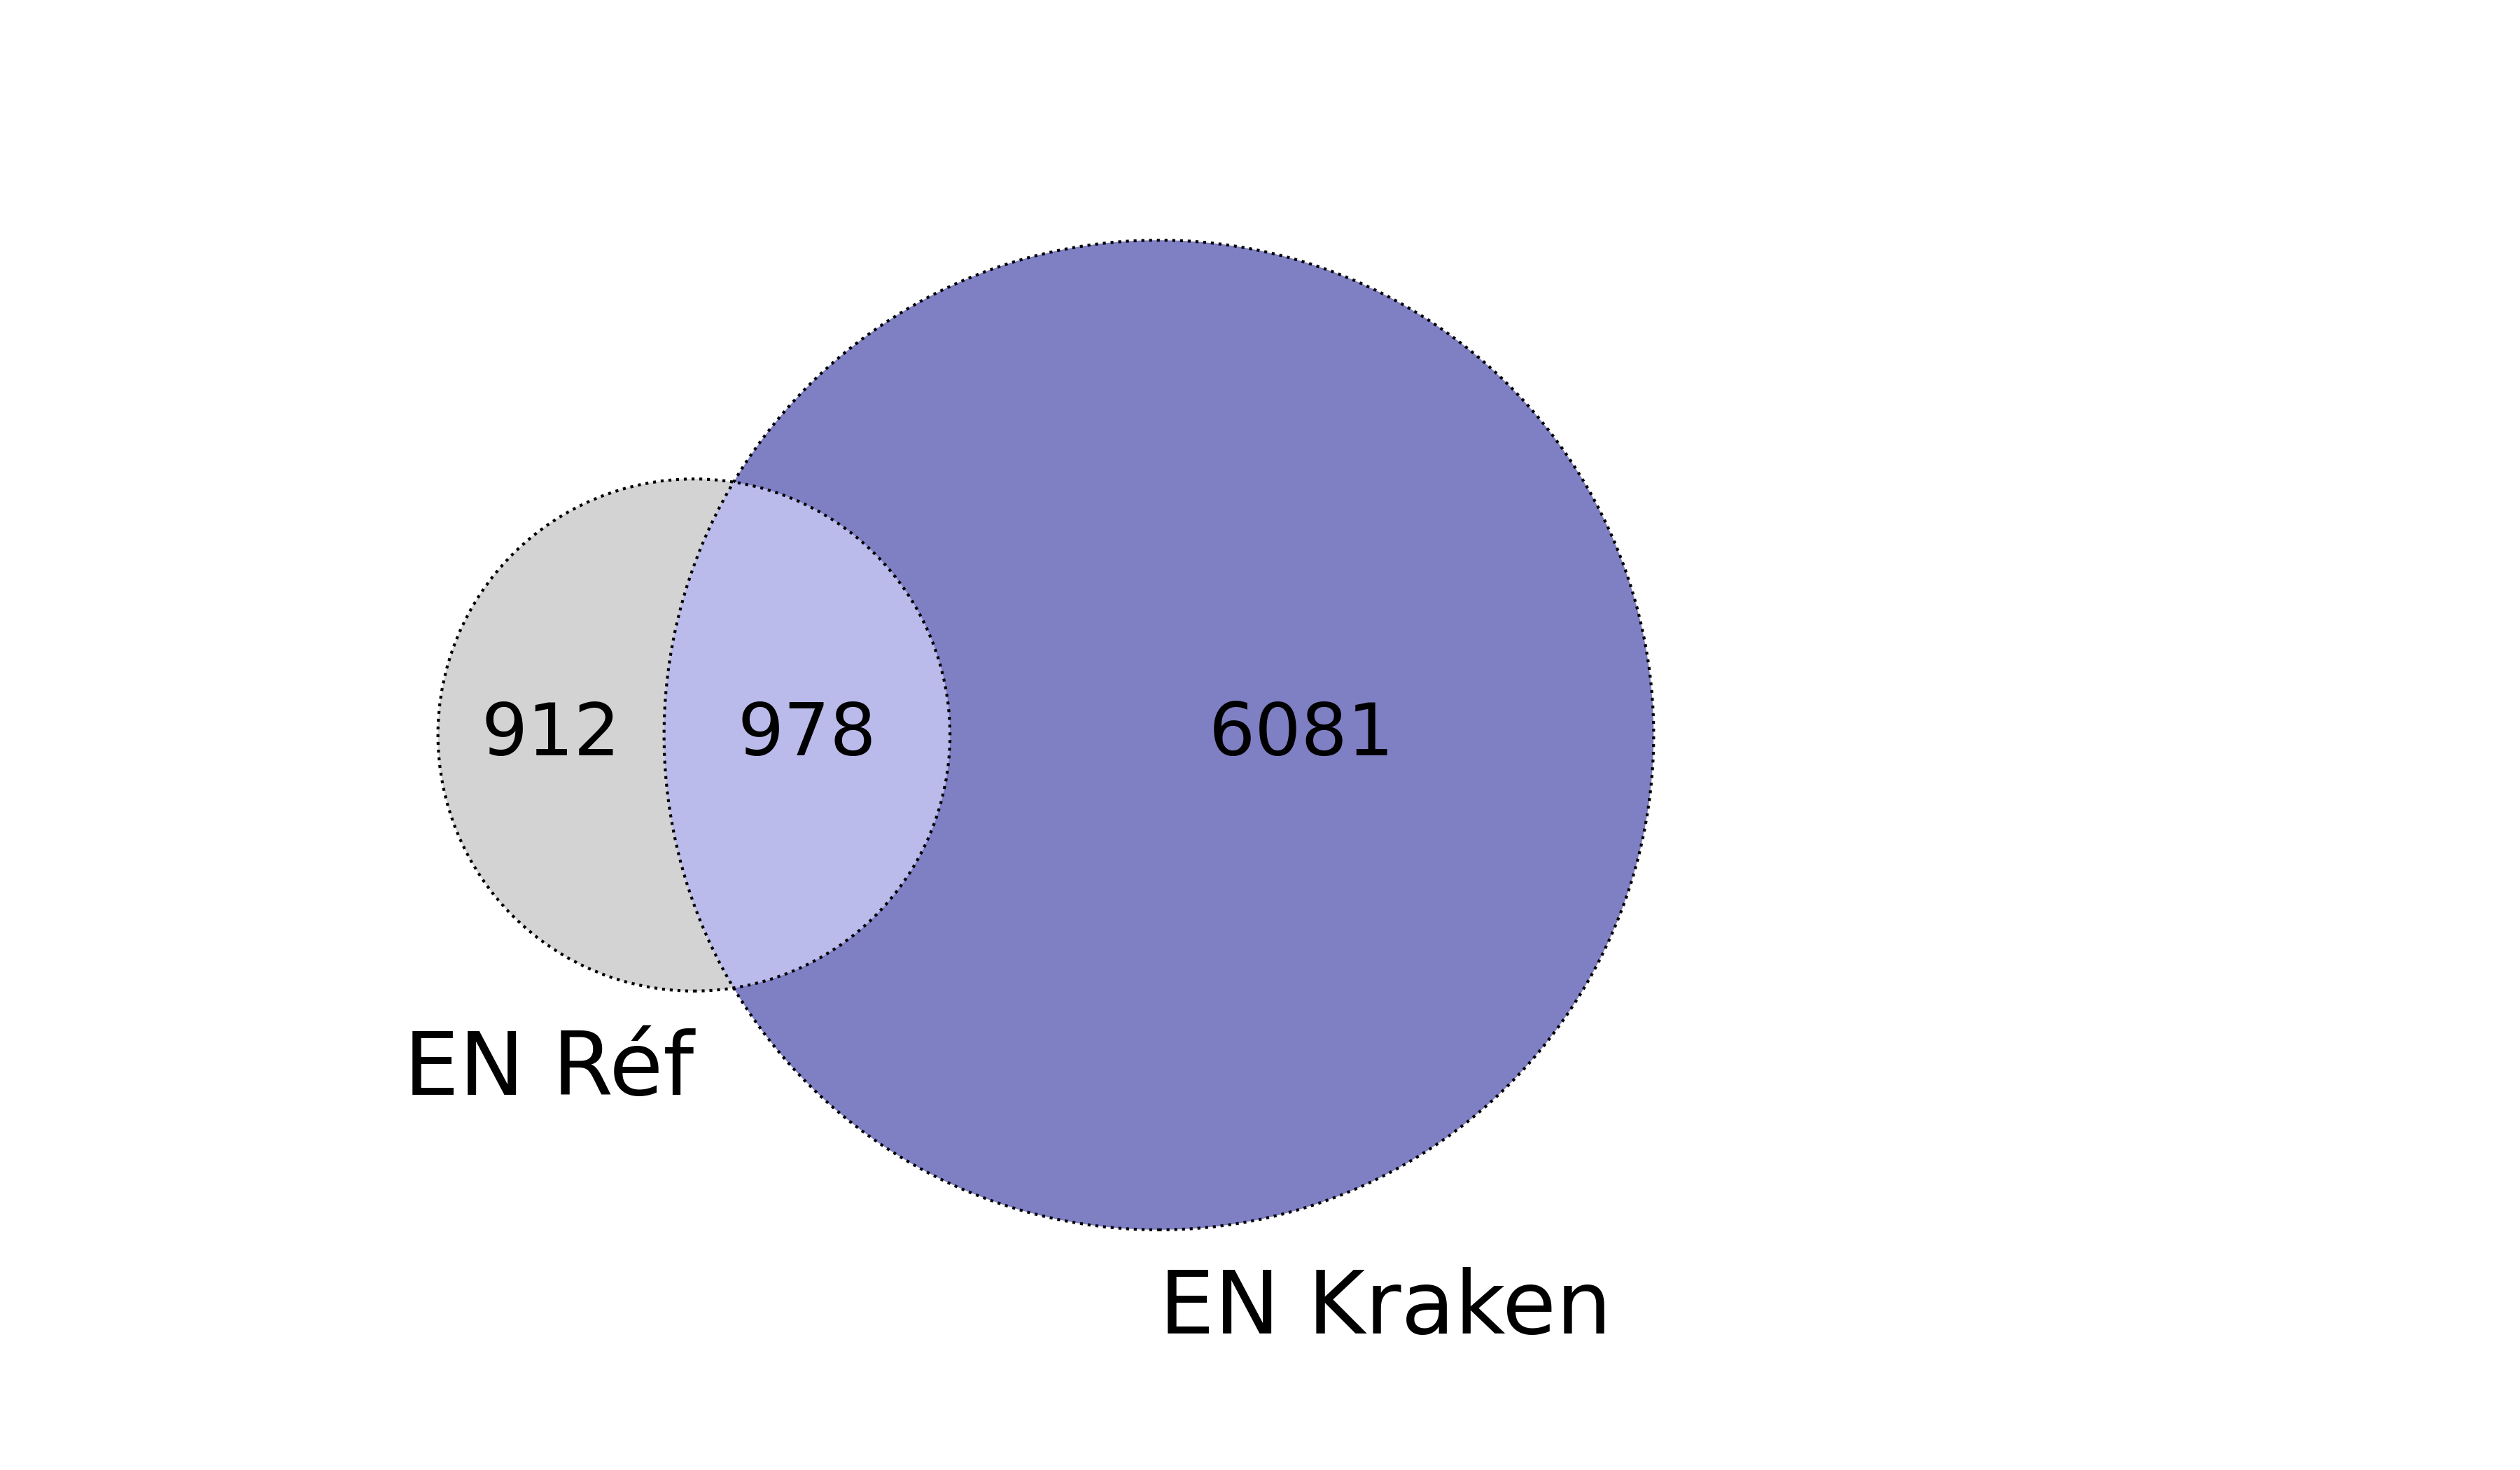
\includegraphics[width=1\textwidth]{IMAGES/INTERSECTIONS_GLOBALES/ELTeCFRA_Kraken_spacy-lg-concat_intersection.png} 
  \caption{Kraken --\texttt{spaCy-lg}}
  \label{fig:ELTeCFRA_Kraken_spacy-lg-concat_intersection}
  \end{subfigure}
  \end{minipage}
  \begin{minipage}{7cm}
  \begin{subfigure}{1\textwidth}
%  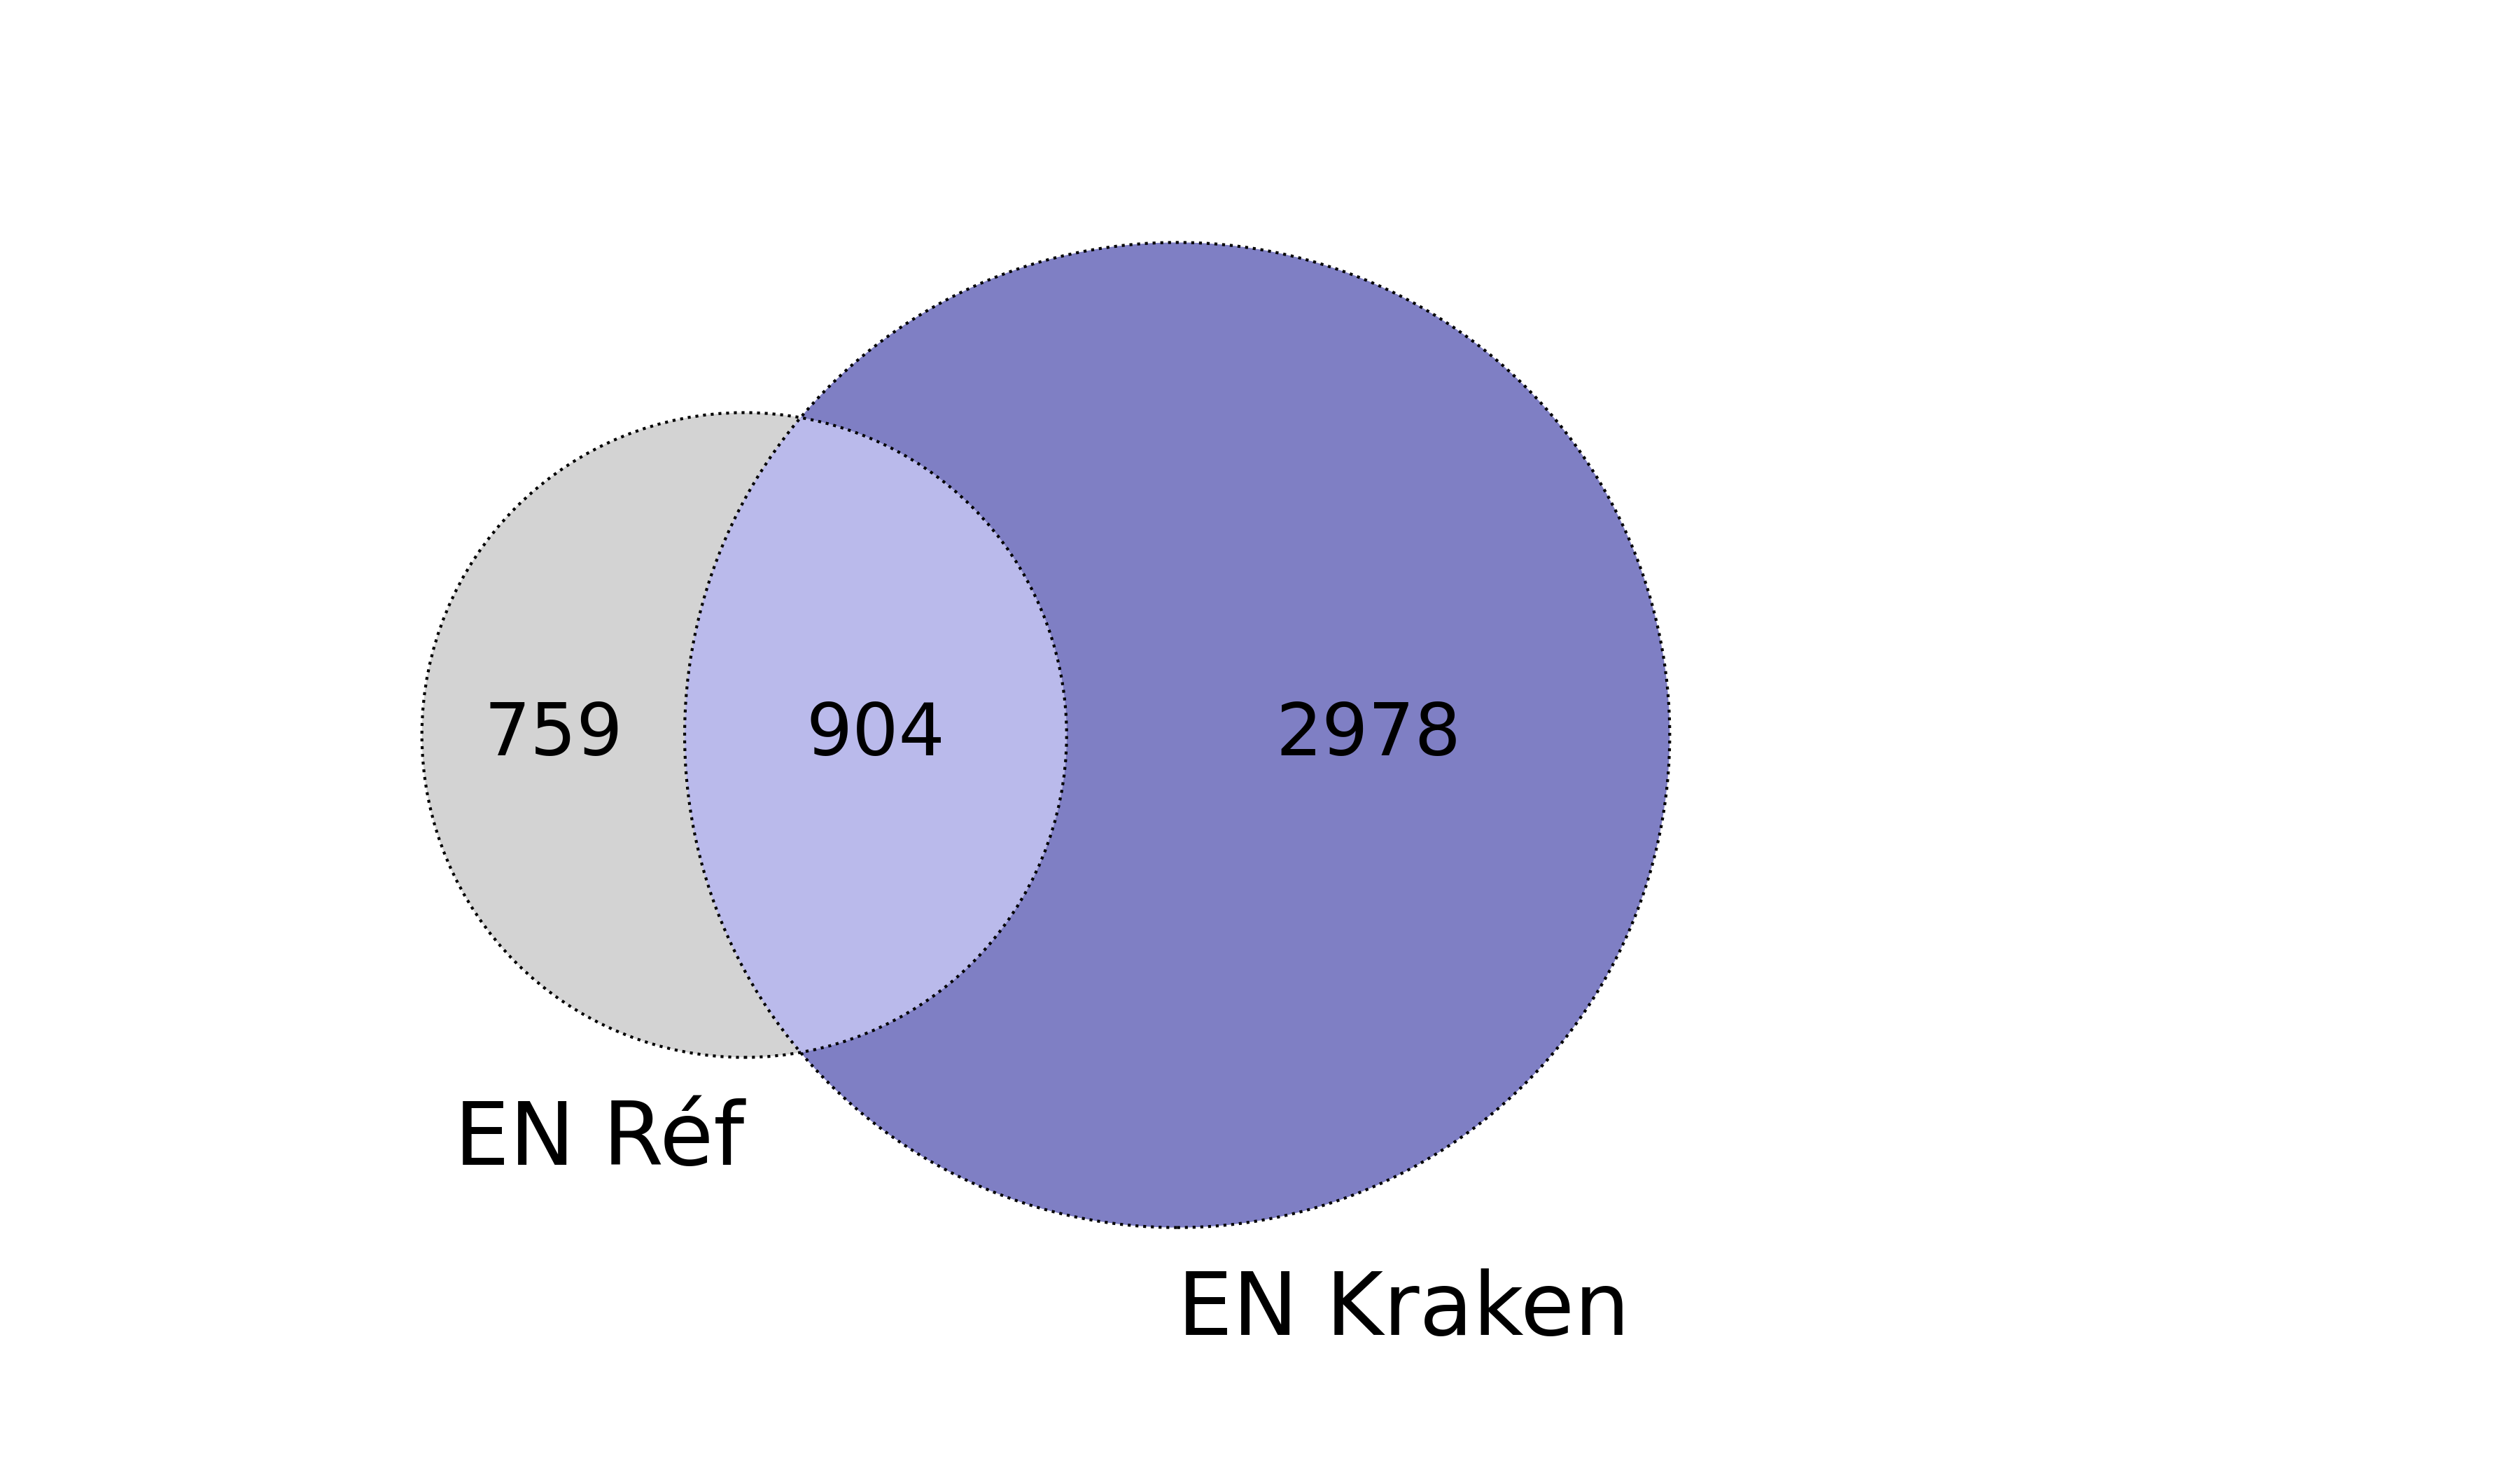
\includegraphics[width=1\textwidth]{IMAGES/INTERSECTIONS_GLOBALES/ELTeCFRA_Kraken_stanza-concat_intersection.png} %%%% ancienne figure 07/02/2024
  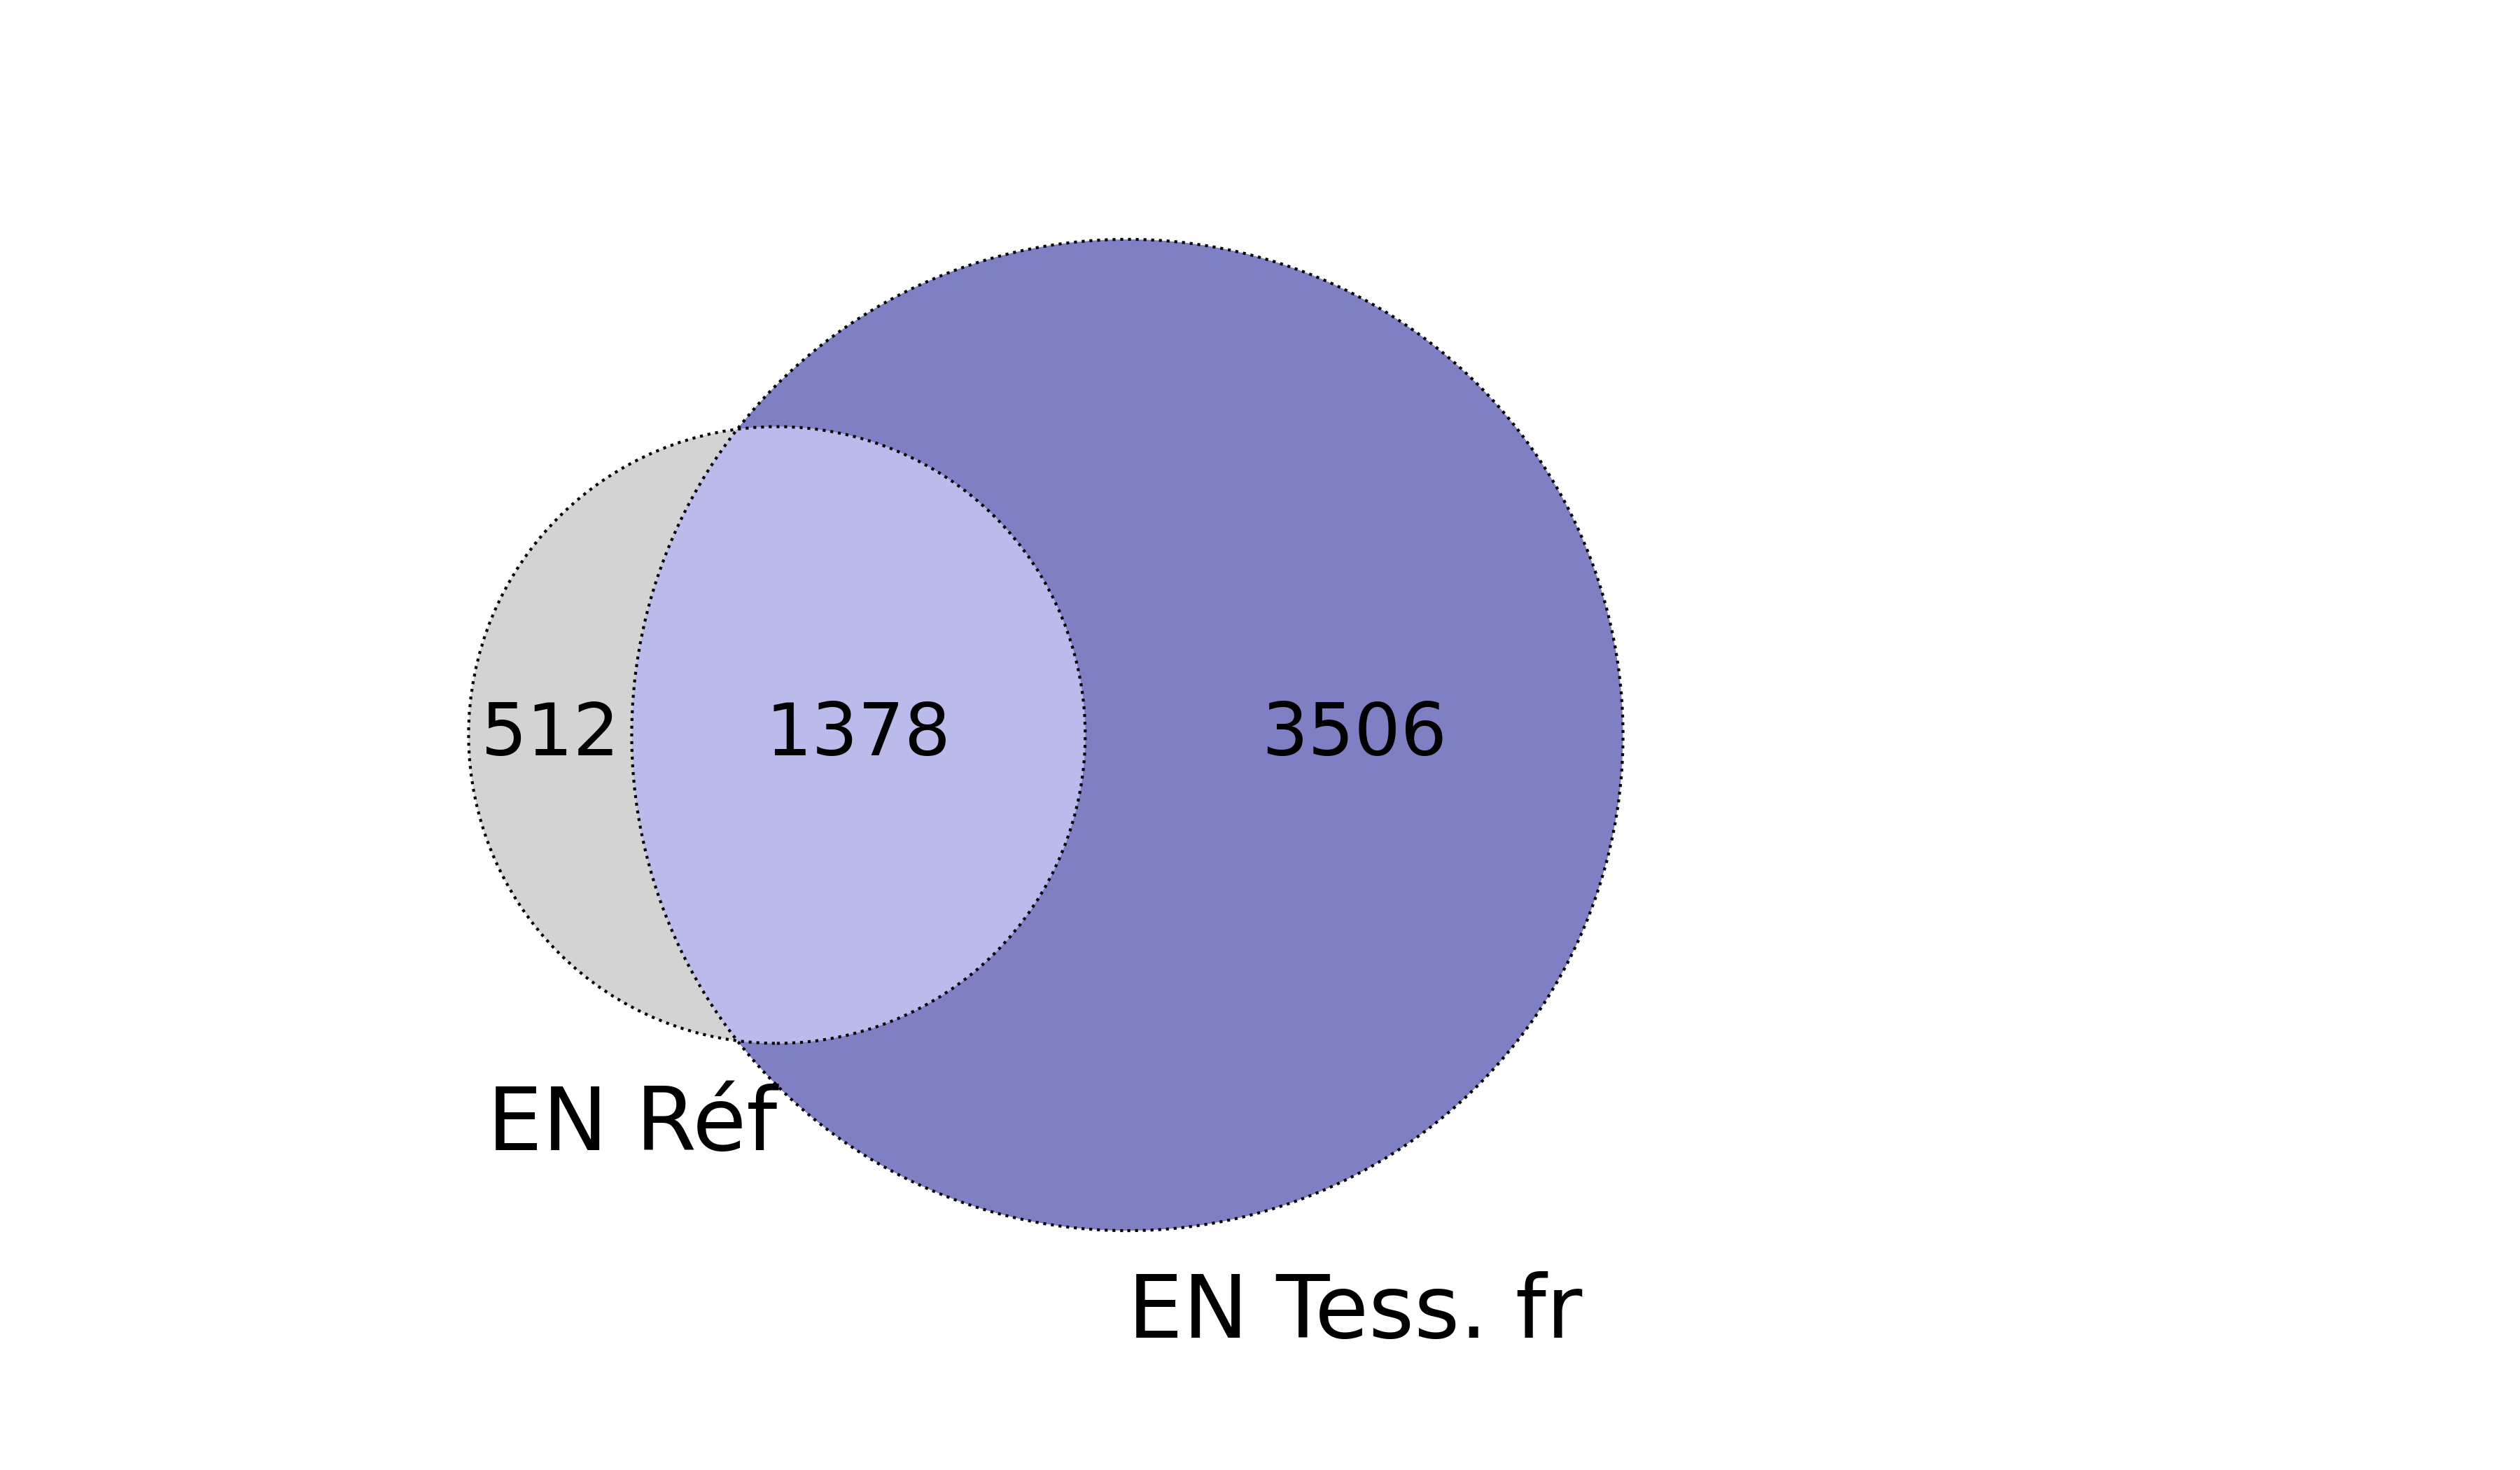
\includegraphics[width=1\textwidth]{IMAGES/INTERSECTIONS_GLOBALES/ELTeCFRA_Tess. fr_spacy-lg-concat_intersection.png}
  \caption{Tess. fr. -- \texttt{spaCy\_lg}}
 % \label{fig:ELTeCFRA_Kraken_stanza-concat_intersection}
  \end{subfigure}
    \end{minipage}
%\begin{minipage}{7cm}
%  \begin{subfigure}{1\textwidth}
%  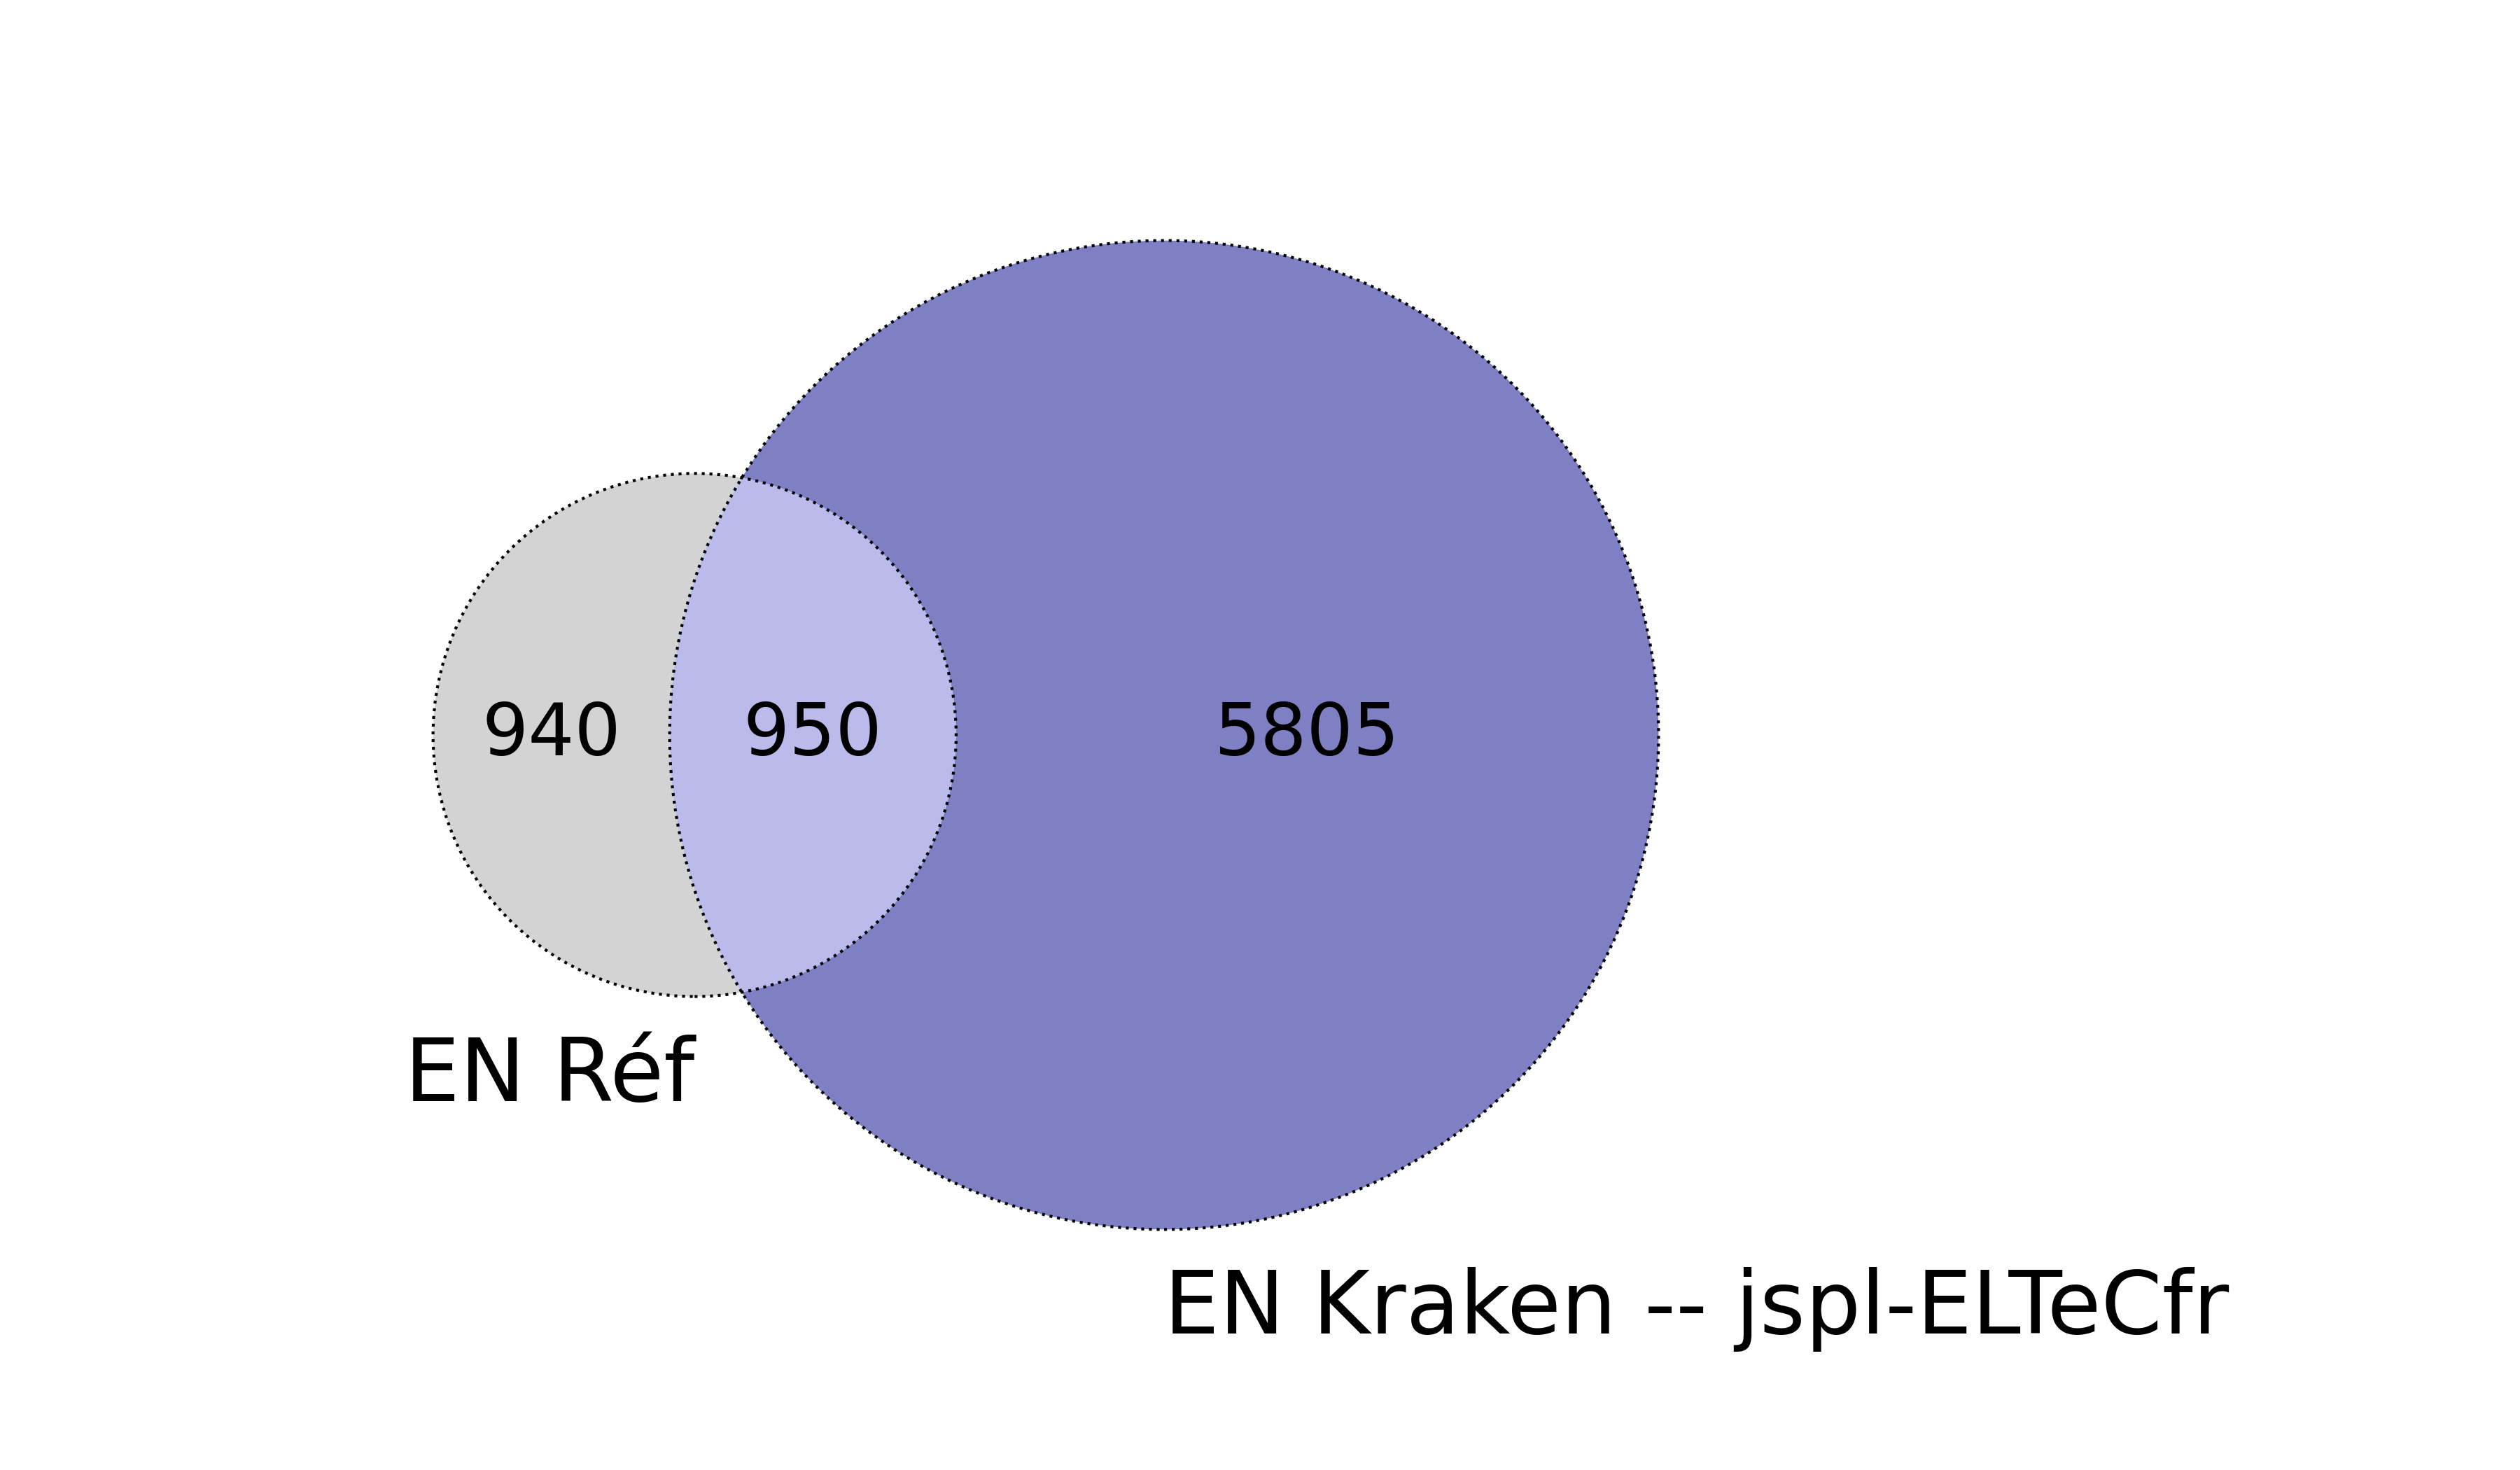
\includegraphics[width=1\textwidth]{IMAGES/INTERSECTIONS_GLOBALES/ELTeCFRA_Kraken -- jspl-ELTeCfr_spacy-lg-concat_intersection.png} 
%  \caption{Kraken corrigé ELTeC-fr -- \texttt{spaCy-lg}}
%  \label{fig:ELTeCFRA_Kraken -- jspl-ELTeCfr_spacy-lg-concat_intersection}
%  \end{subfigure}
%  \end{minipage}
%  \begin{minipage}{7cm}
%  \begin{subfigure}{1\textwidth}
%  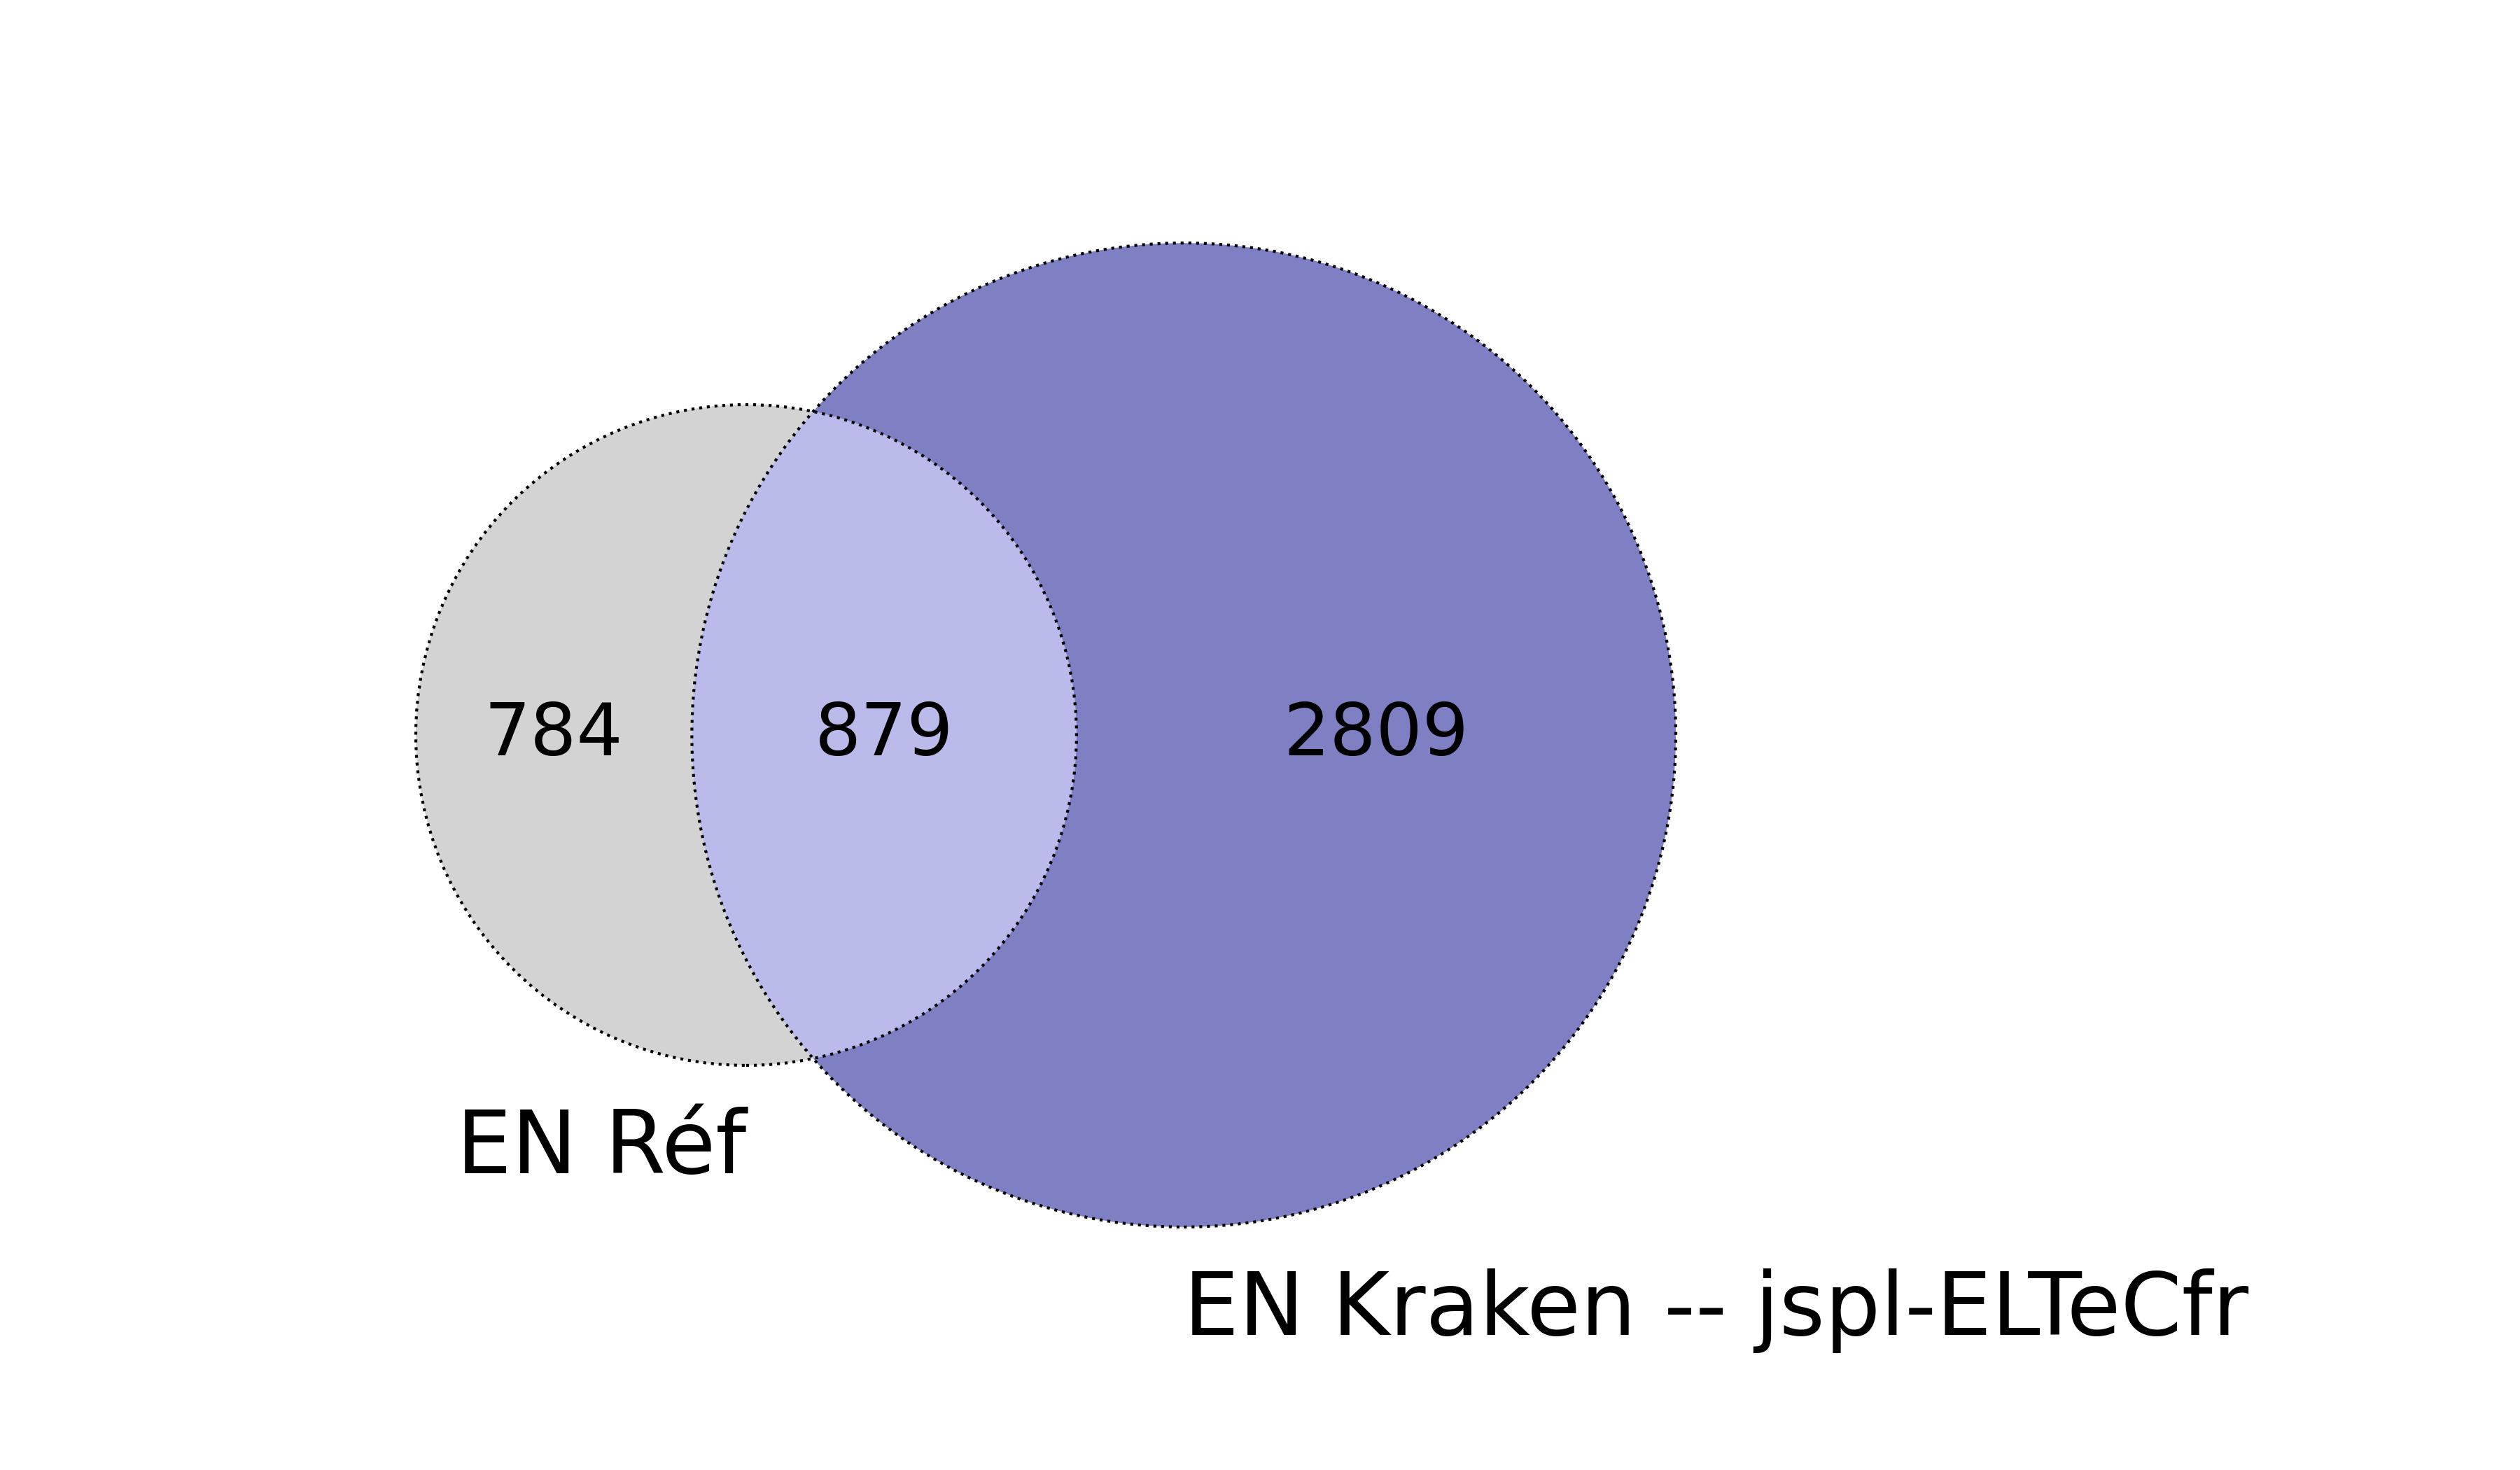
\includegraphics[width=1\textwidth]{IMAGES/INTERSECTIONS_GLOBALES/ELTeCFRA_Kraken -- jspl-ELTeCfr_stanza-concat_intersection.png}
%  \caption{Kraken corrigé ELTeC-fr -- \texttt{stanza}}
%  \label{fig:ELTeCFRA_Kraken -- jspl-ELTeCFR_stanza-concat_intersection}
%  \end{subfigure}
%    \end{minipage}
\caption{Intersections pour les configurations Kraken-\texttt{spaCy\_lg} et Tess. fr.-\texttt{spaCy\_lg}, pour le sous-corpus ELTeC français.}
%\label{fig:intersection_globale-kraken}
\label{fig:intersection_globale-kraken-tess}
\end{figure}

%%%%%%%%%%%% ancienne sous-figure 07/02/2024
%\begin{figure}[h!]
%    \begin{minipage}{7cm}
%  \begin{subfigure}{1\textwidth}
%  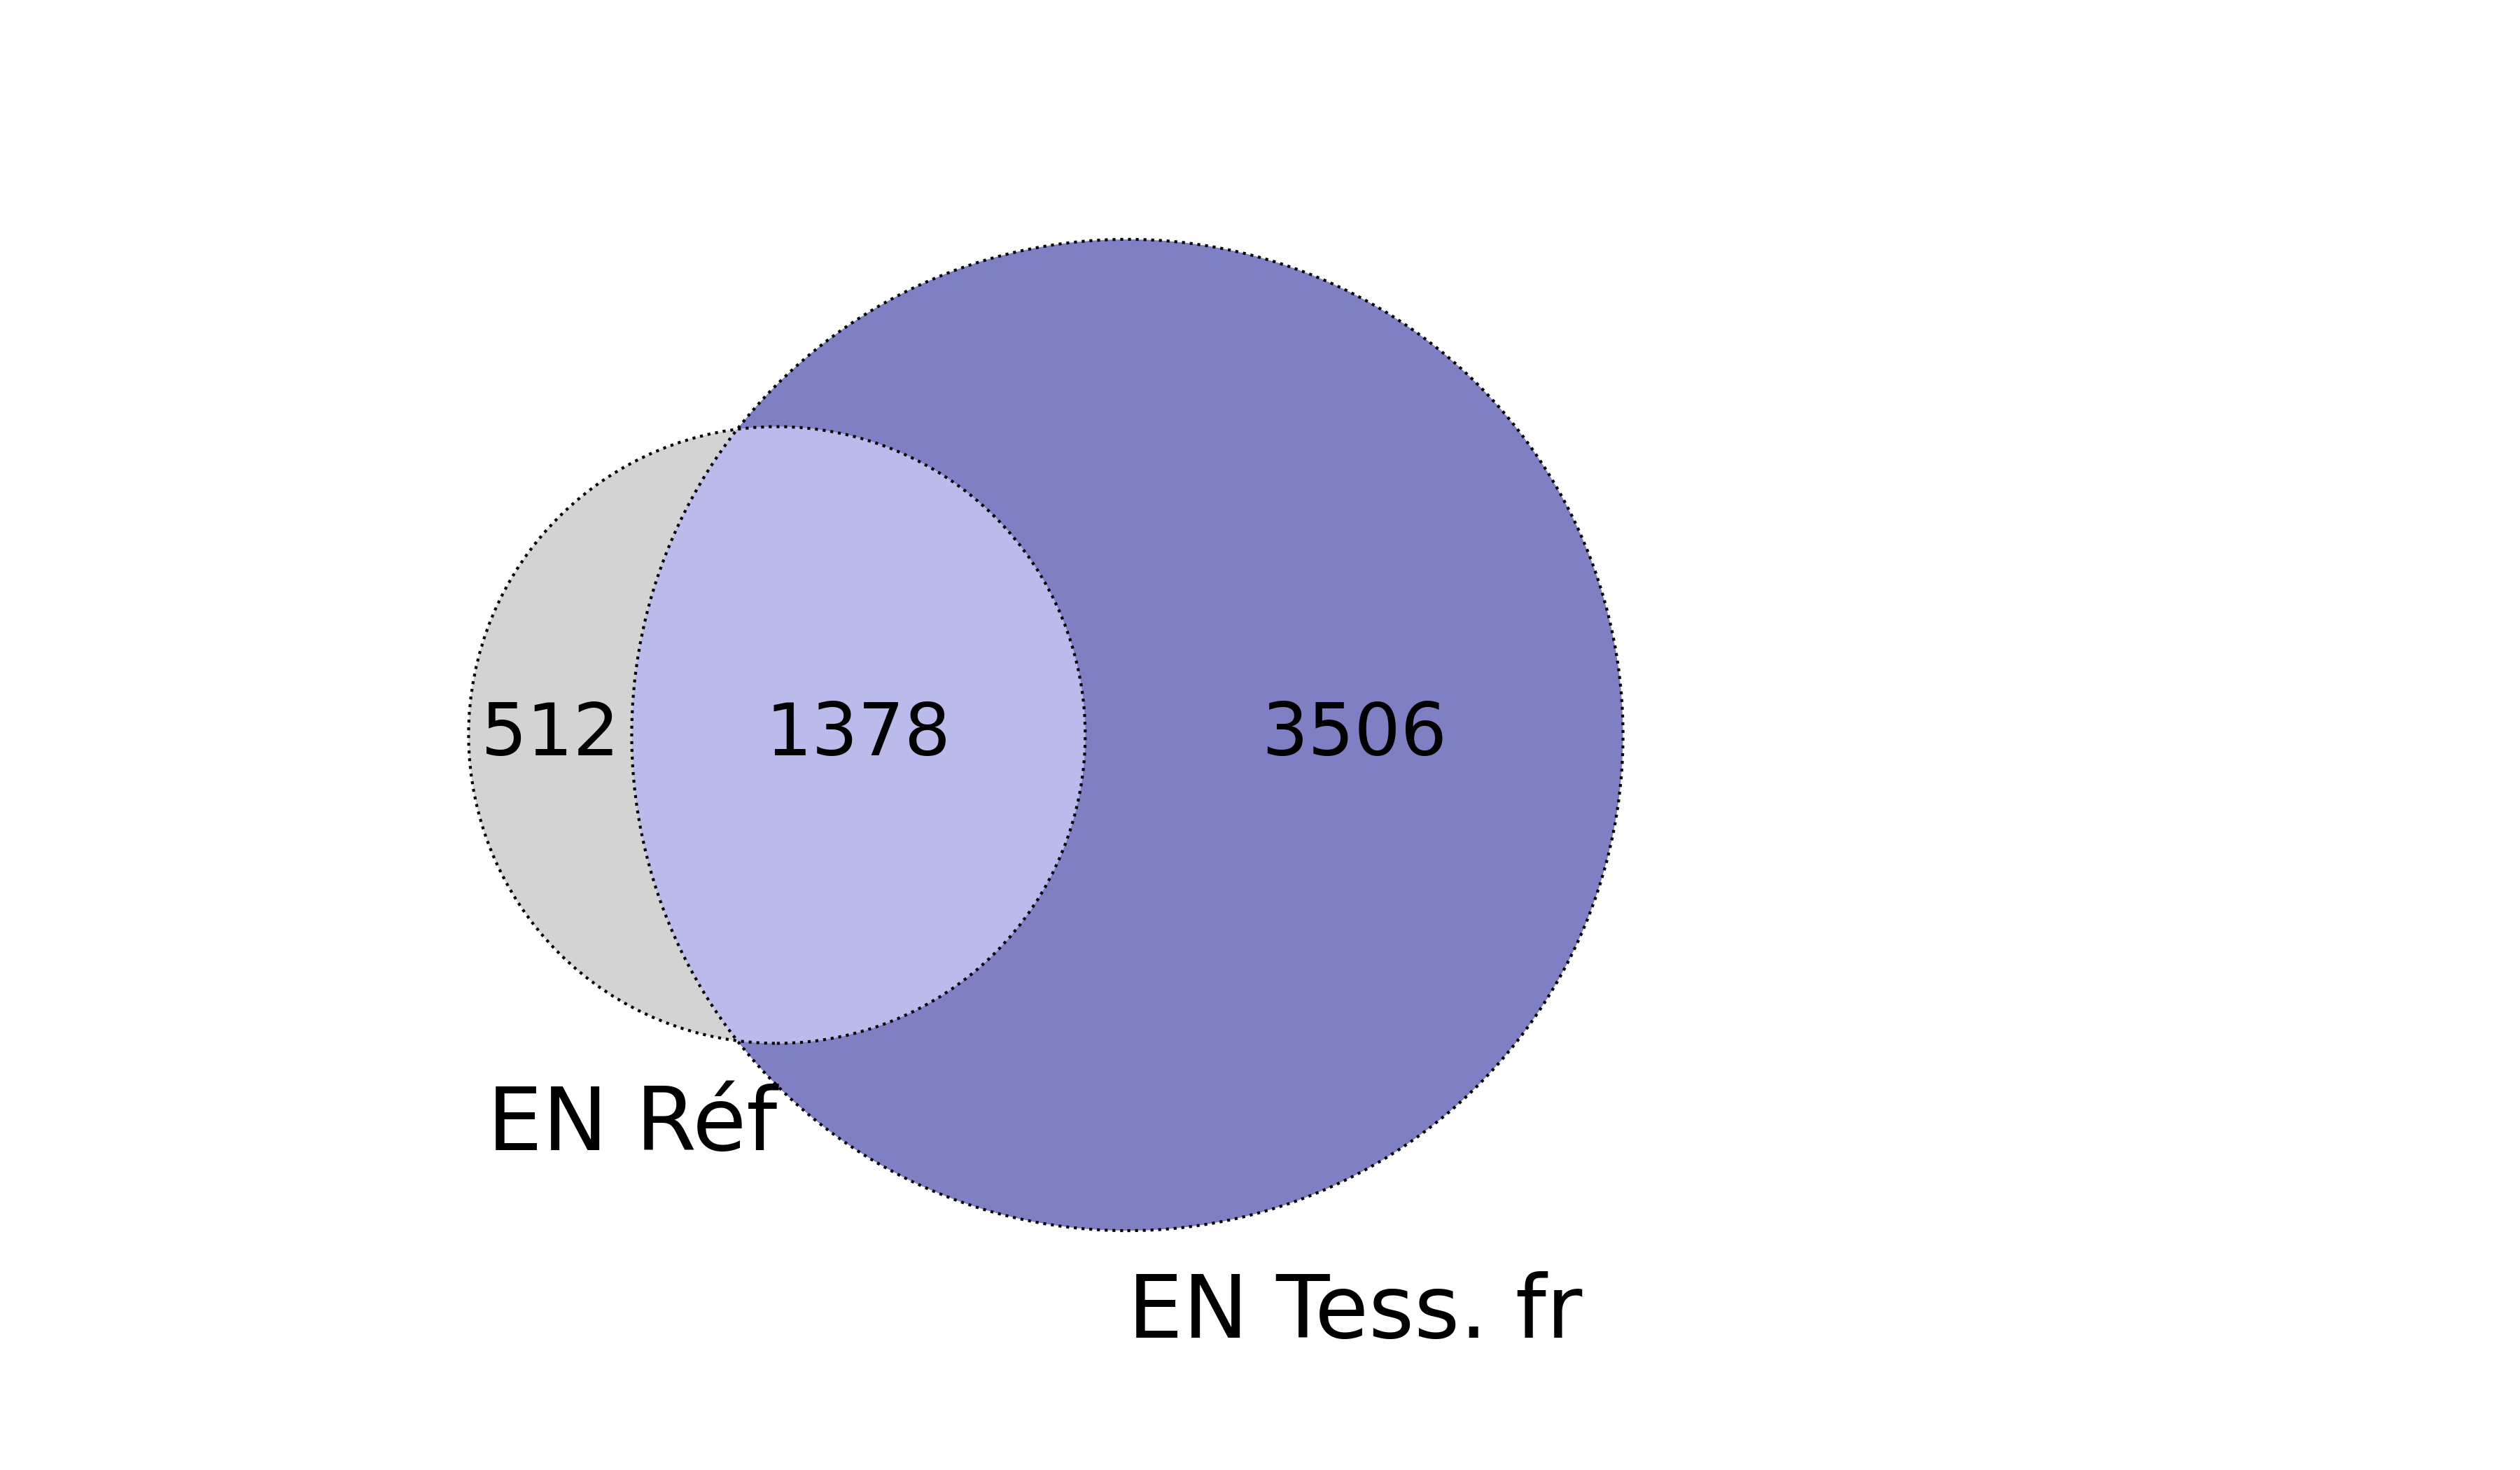
\includegraphics[width=1\textwidth]{IMAGES/INTERSECTIONS_GLOBALES/ELTeCFRA_Tess. fr_spacy-lg-concat_intersection.png} 
%  \caption{Tess. fr. --\texttt{spaCy\_lg}}
%  \label{fig:ELTeCFRA_Tess. fr_spacy-lg-concat_intersection}
%  \end{subfigure}
%  \end{minipage}
%  \begin{minipage}{7cm}
%  \begin{subfigure}{1\textwidth}
%  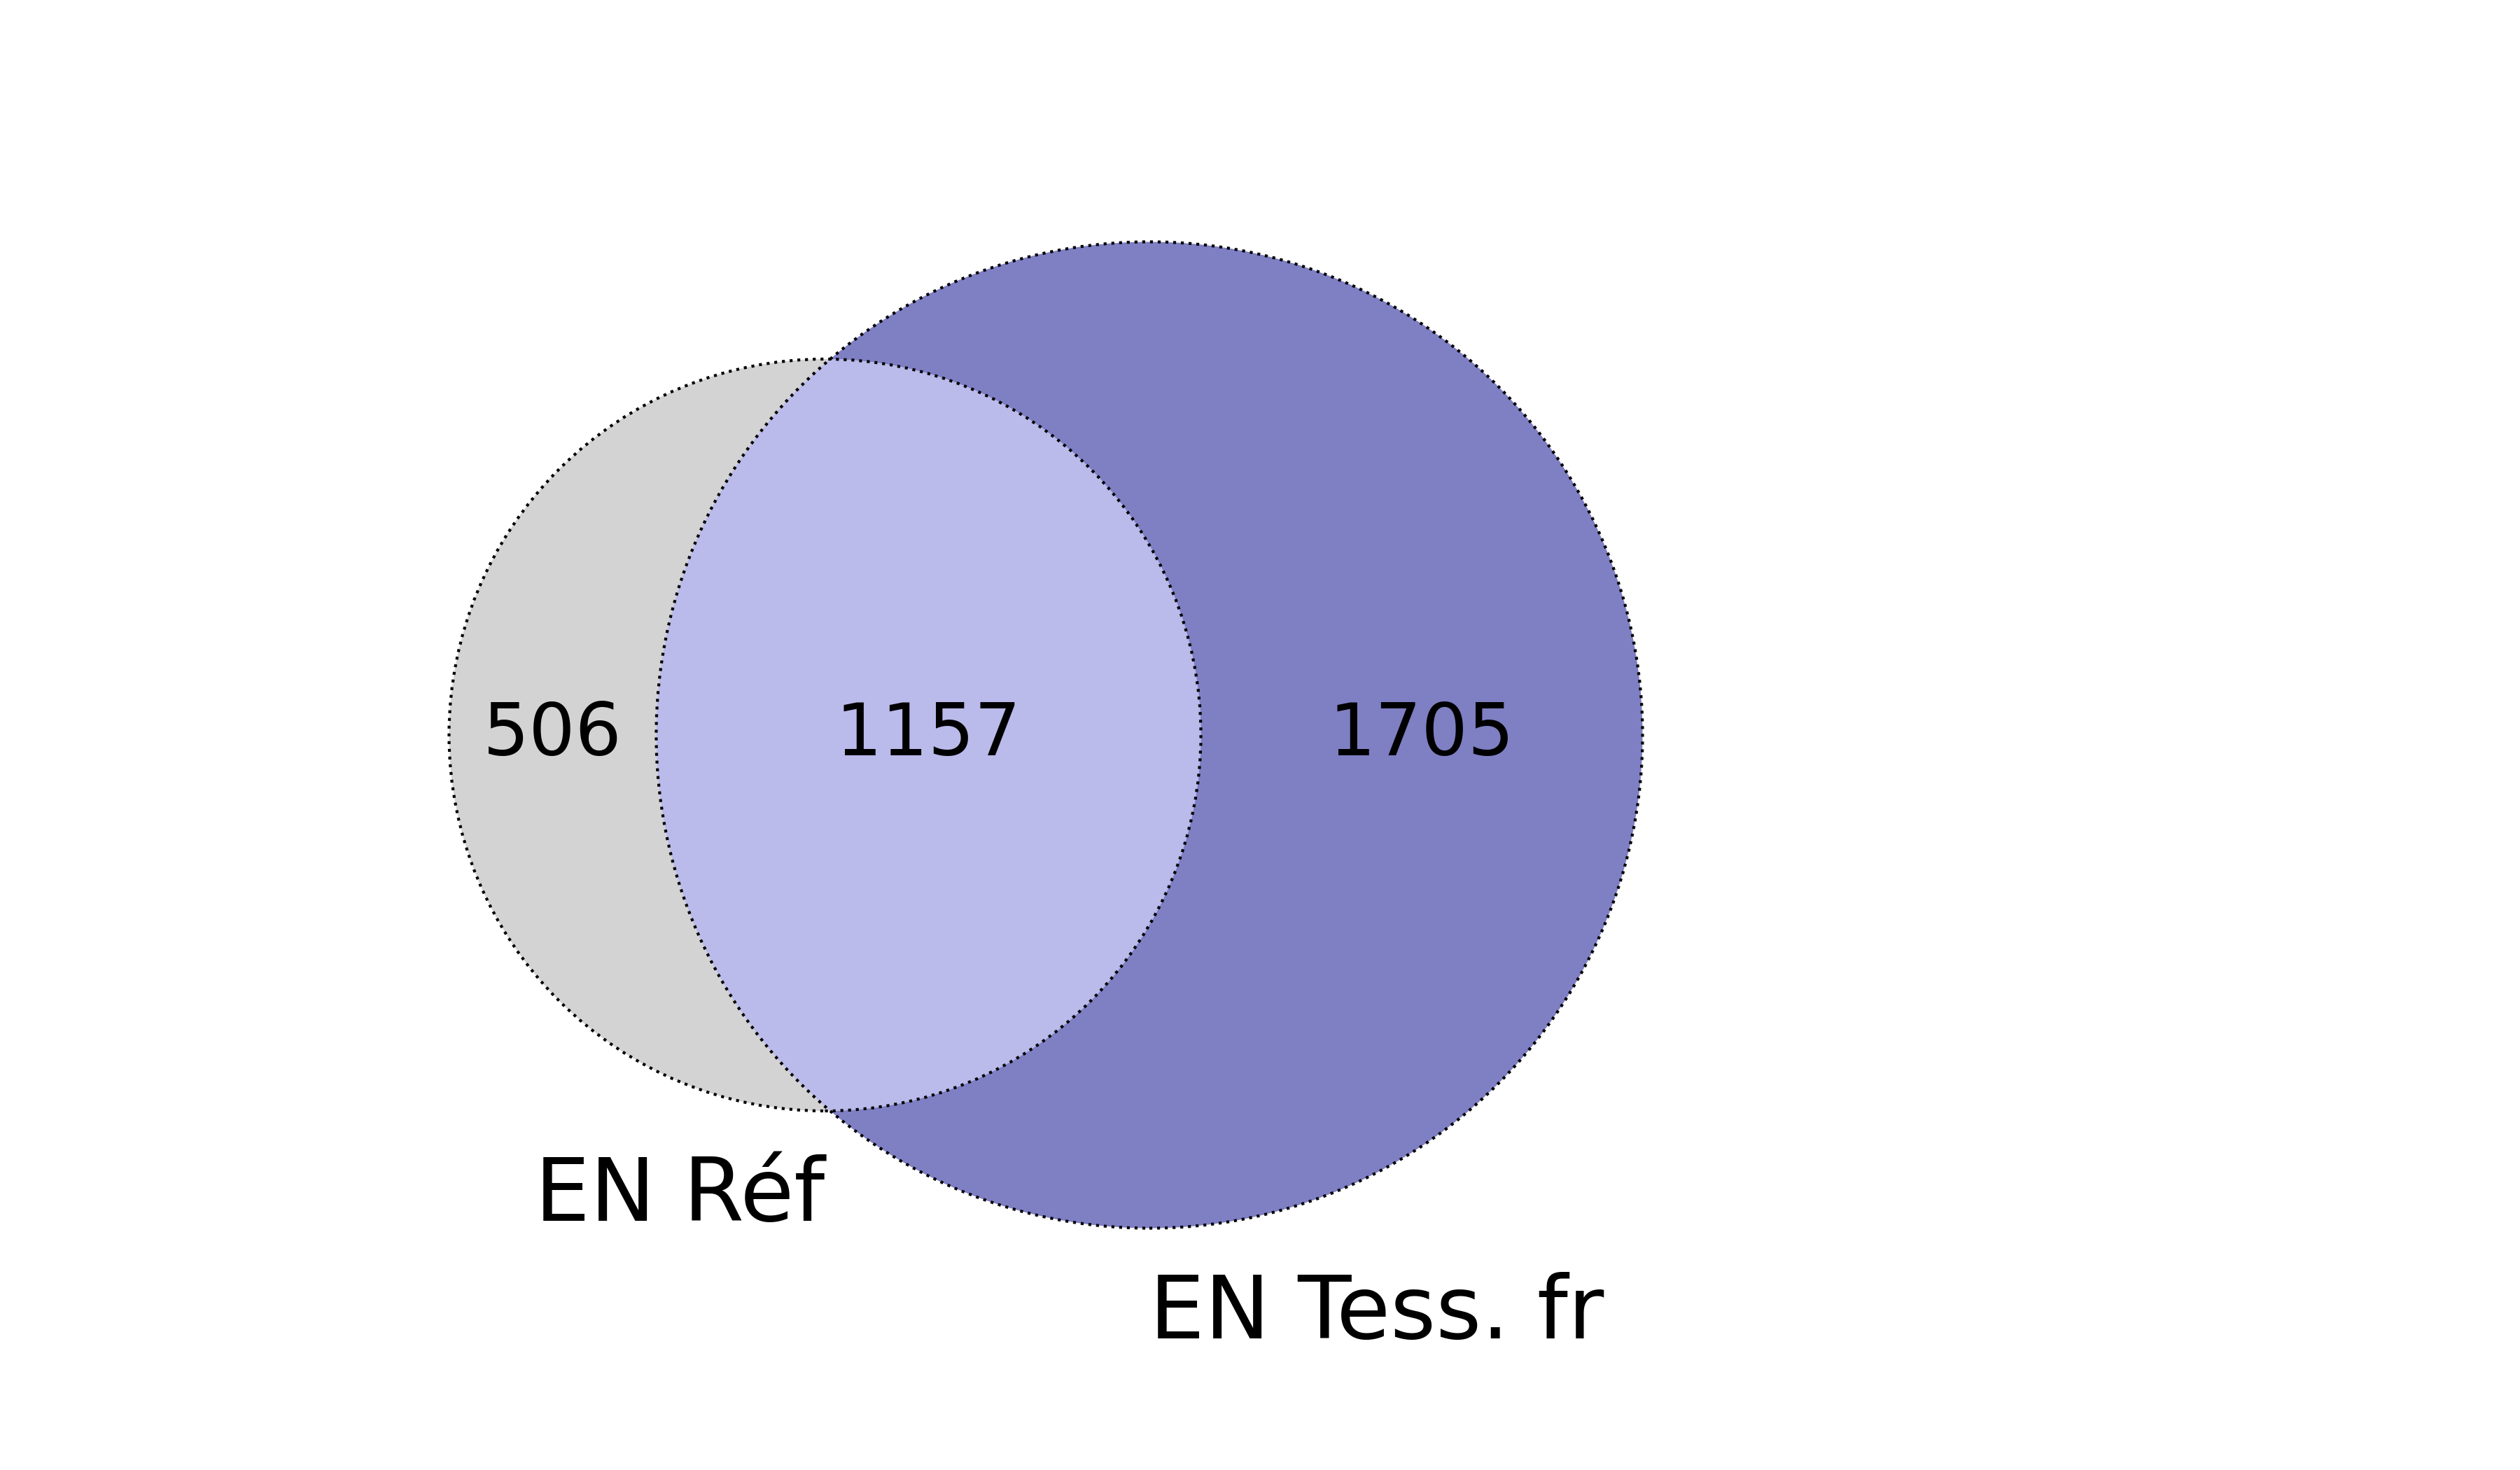
\includegraphics[width=1\textwidth]{IMAGES/INTERSECTIONS_GLOBALES/ELTeCFRA_Tess. fr_stanza-concat_intersection.png}
%  \caption{Tess. fr. -- \texttt{stanza}}
% % \label{fig:ELTeCFRA_Tess. fr_stanza-concat_intersection}
%  \end{subfigure}
%    \end{minipage}

%\begin{minipage}{7cm}
%  \begin{subfigure}{1\textwidth}
%  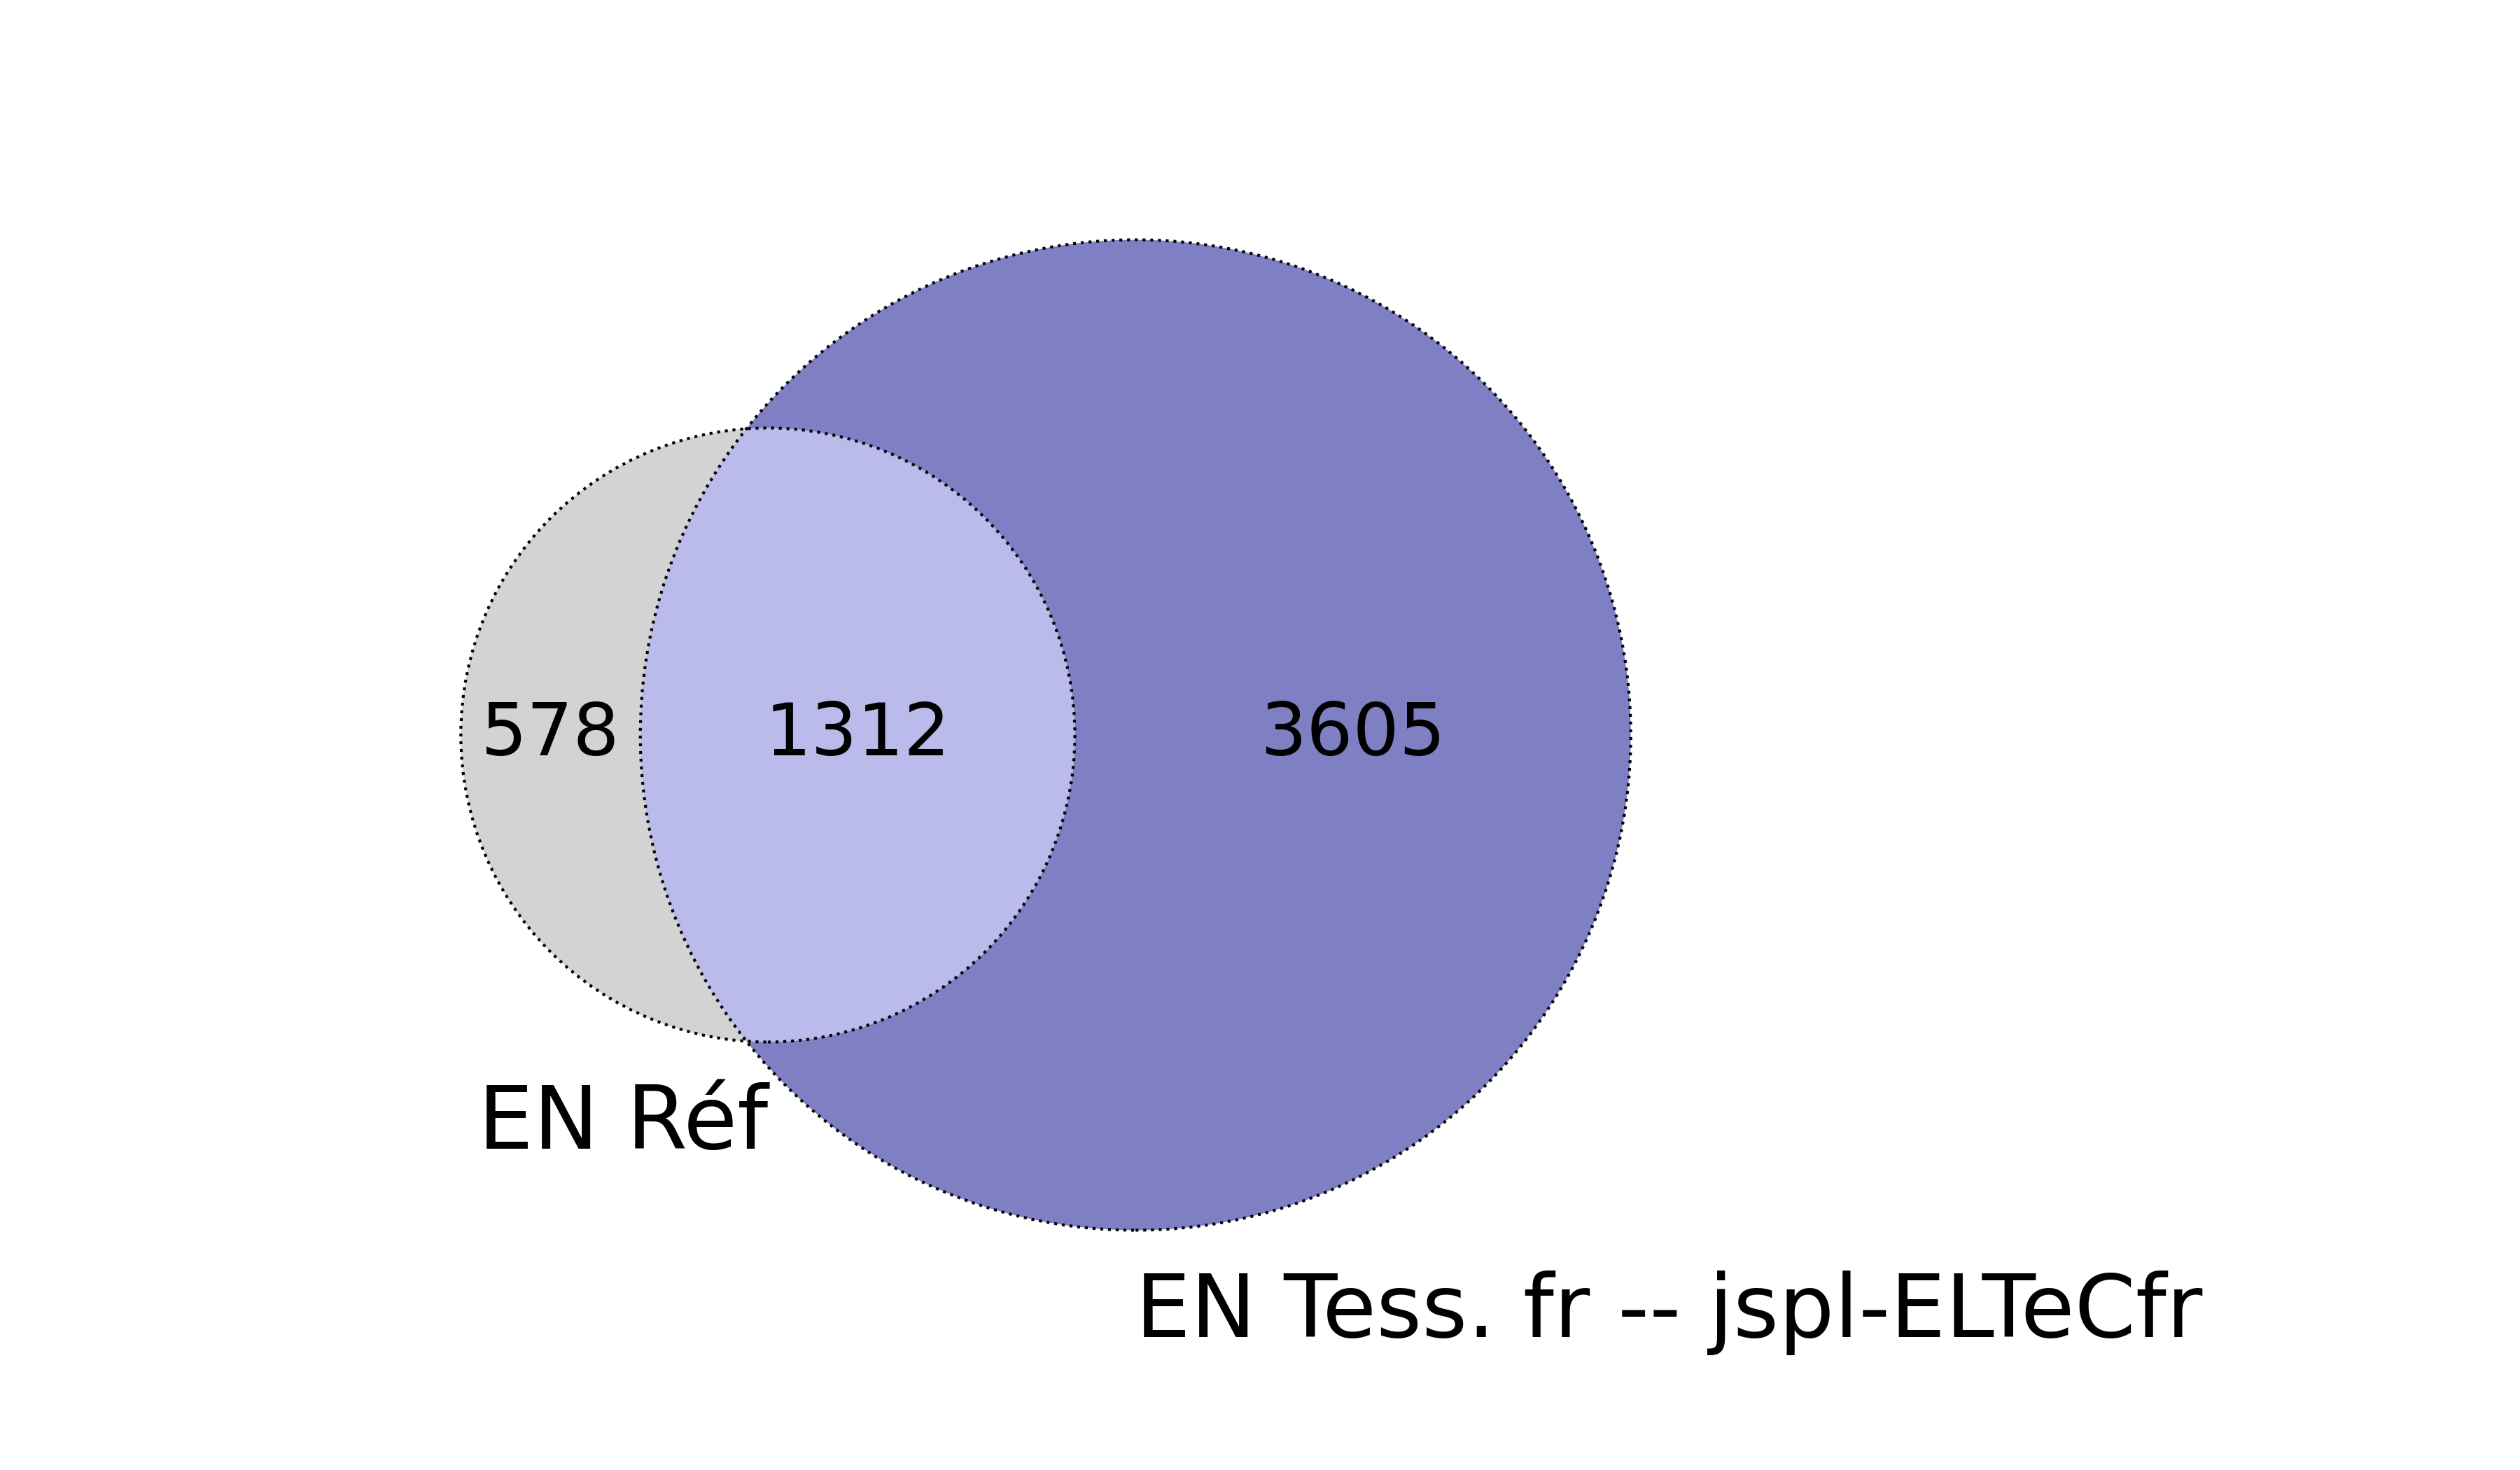
\includegraphics[width=1\textwidth]{IMAGES/INTERSECTIONS_GLOBALES/ELTeCFRA_Tess. fr -- jspl-ELTeCfr_spacy-lg-concat_intersection.png} 
%  \caption{Tess. fr. corrigé -- \texttt{spaCy\_lg}}
%  \label{fig:ELTeCFRA_Tess. fr -- jspl-ELTeCfr_spacy-lg-concat_intersection}
%  \end{subfigure}
% \end{minipage}
%  \begin{minipage}{7cm}
%  \begin{subfigure}{1\textwidth}
%  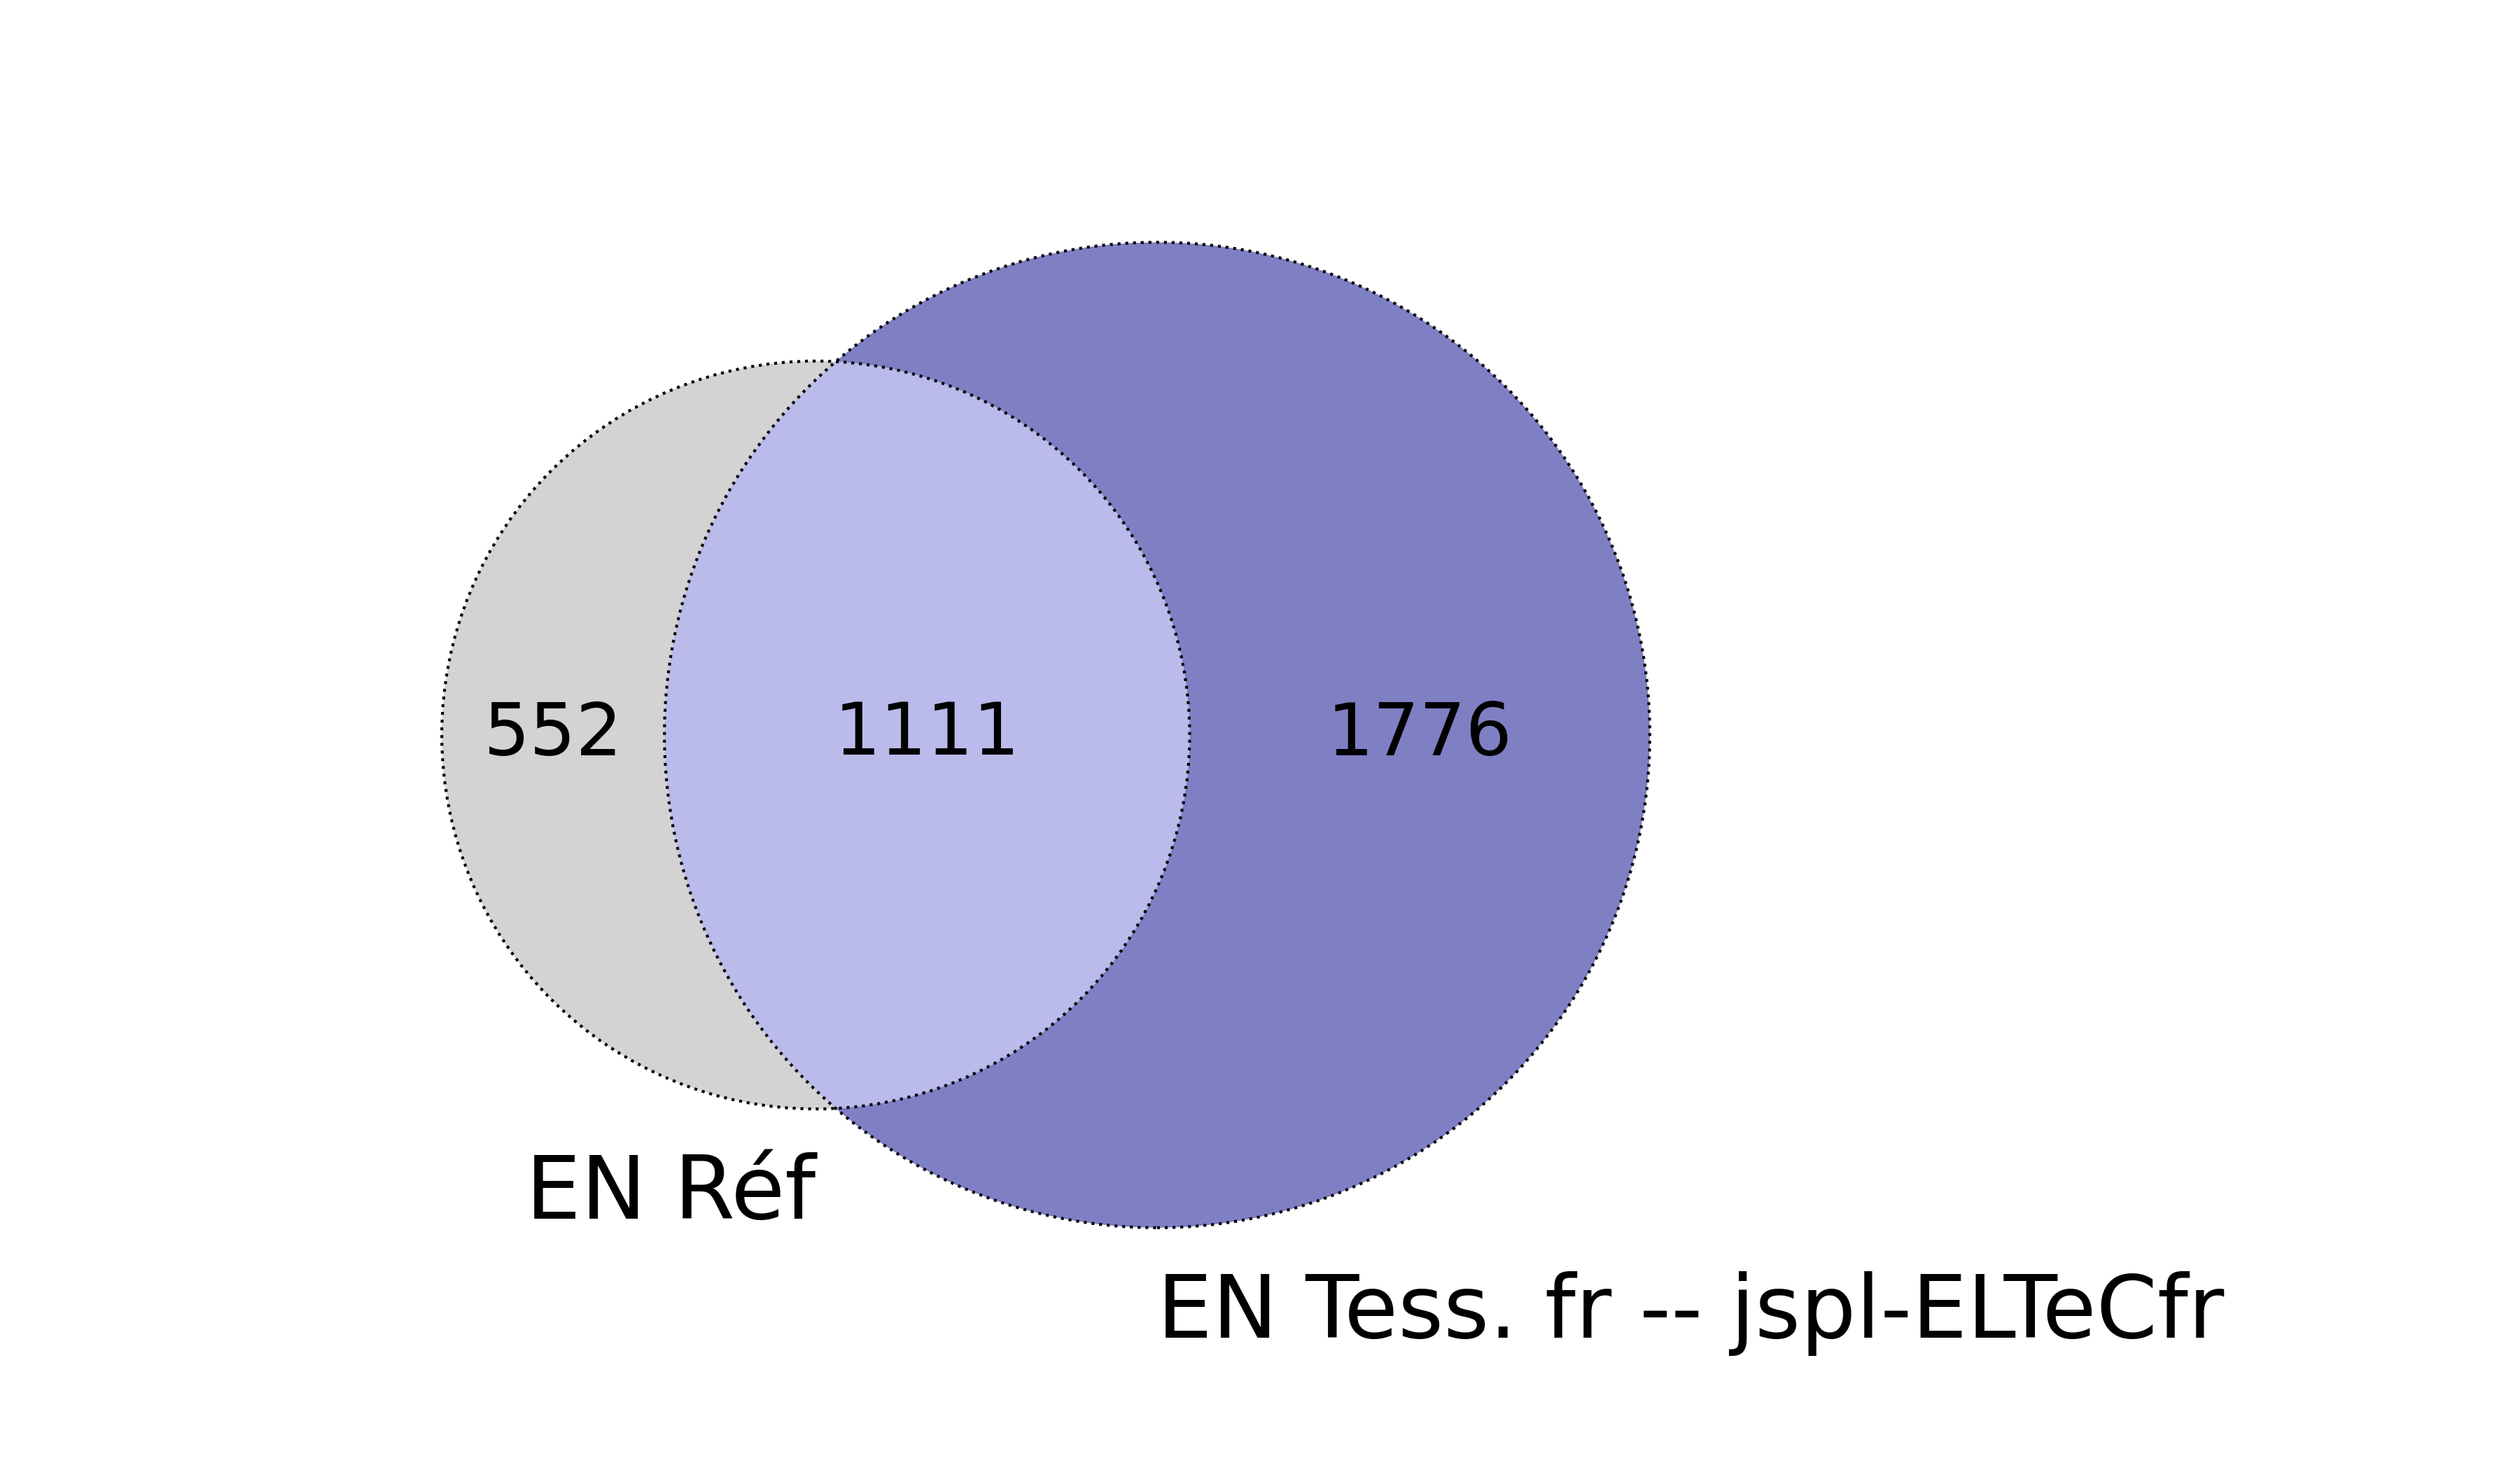
\includegraphics[width=1\textwidth]{IMAGES/INTERSECTIONS_GLOBALES/ELTeCFRA_Tess. fr -- jspl-ELTeCfr_stanza-concat_intersection.png}
%  \caption{Tess. fr. corrigé -- \texttt{stanza}}
%  \label{fig:ELTeCFRA_Tess. fr -- jspl-ELTeCfr_stanza-concat_intersection}
%  \end{subfigure}
%    \end{minipage}
%\begin{minipage}{7cm}
%  \begin{subfigure}{1\textwidth}
%  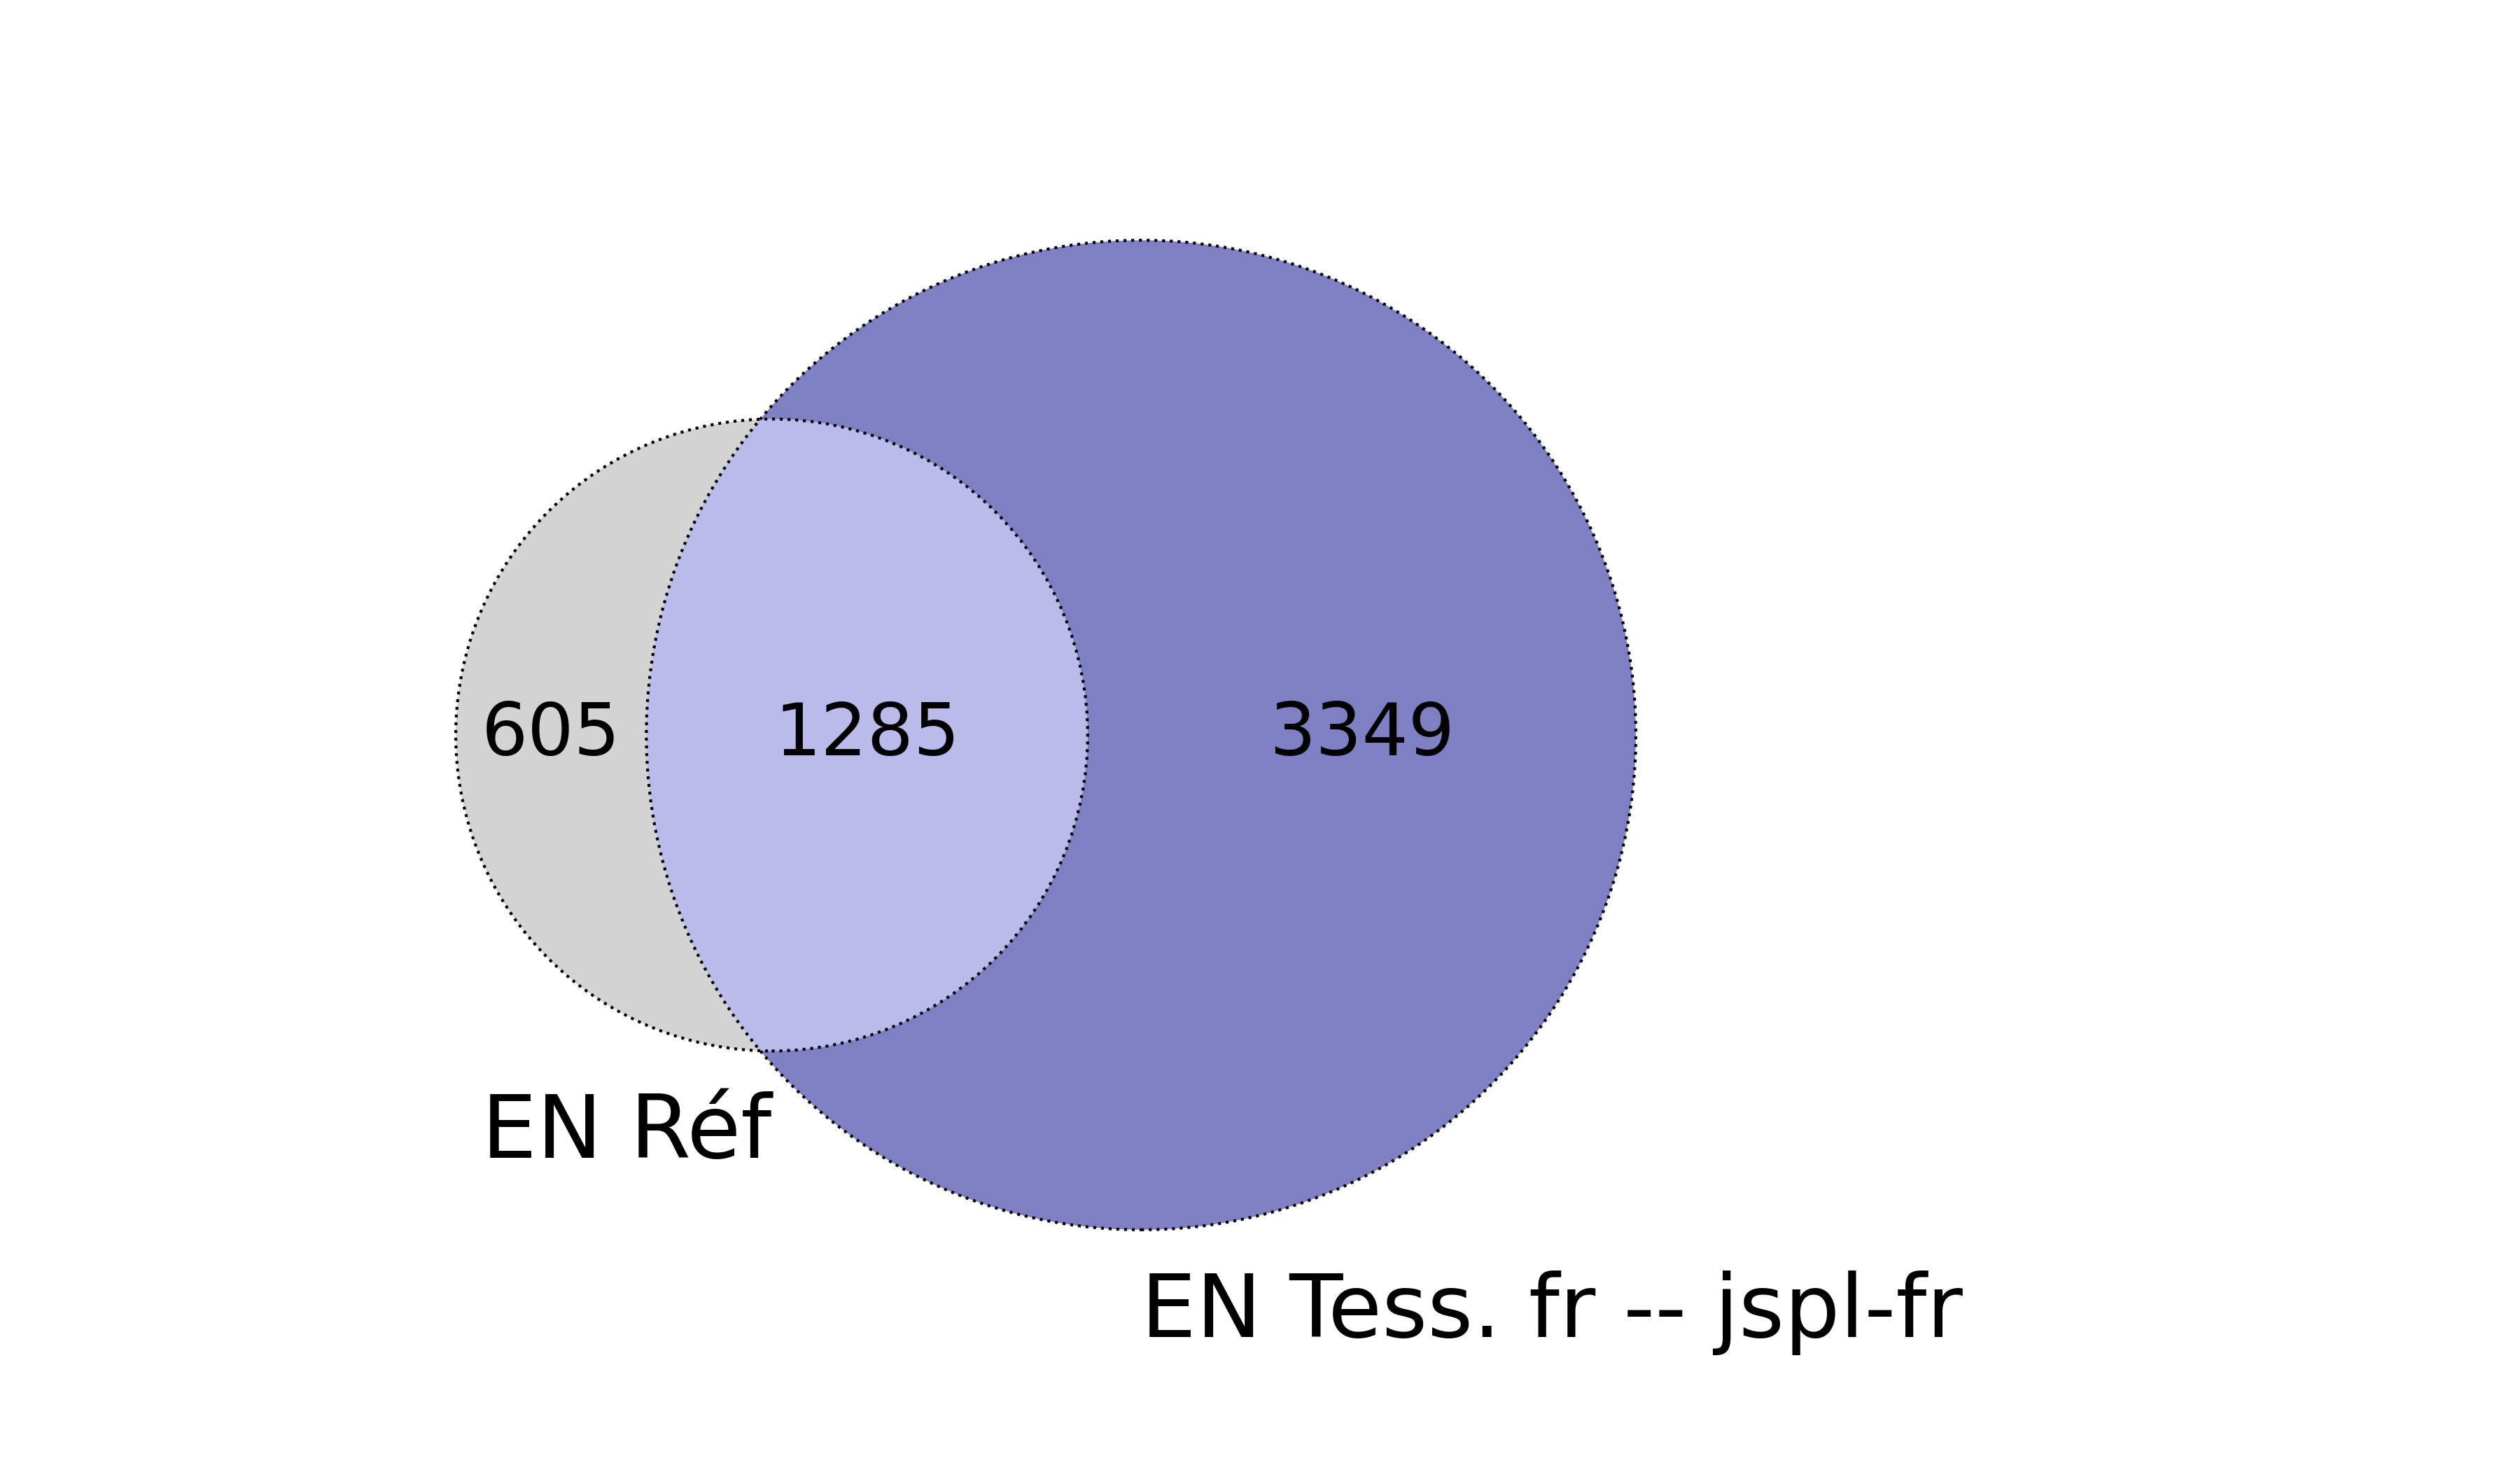
\includegraphics[width=1\textwidth]{IMAGES/INTERSECTIONS_GLOBALES/ELTeCFRA_Tess. fr -- jspl-fr_spacy-lg-concat_intersection.png} 
%  \caption{Tess. fr. corrigé -- \texttt{spaCy\_lg}}
%  \label{fig:ELTeCFRA_Tess. fr -- jspl-fr_spacy-lg-concat_intersection}
%  \end{subfigure}
%  \end{minipage}
%  \begin{minipage}{7cm}
%  \begin{subfigure}{1\textwidth}
%  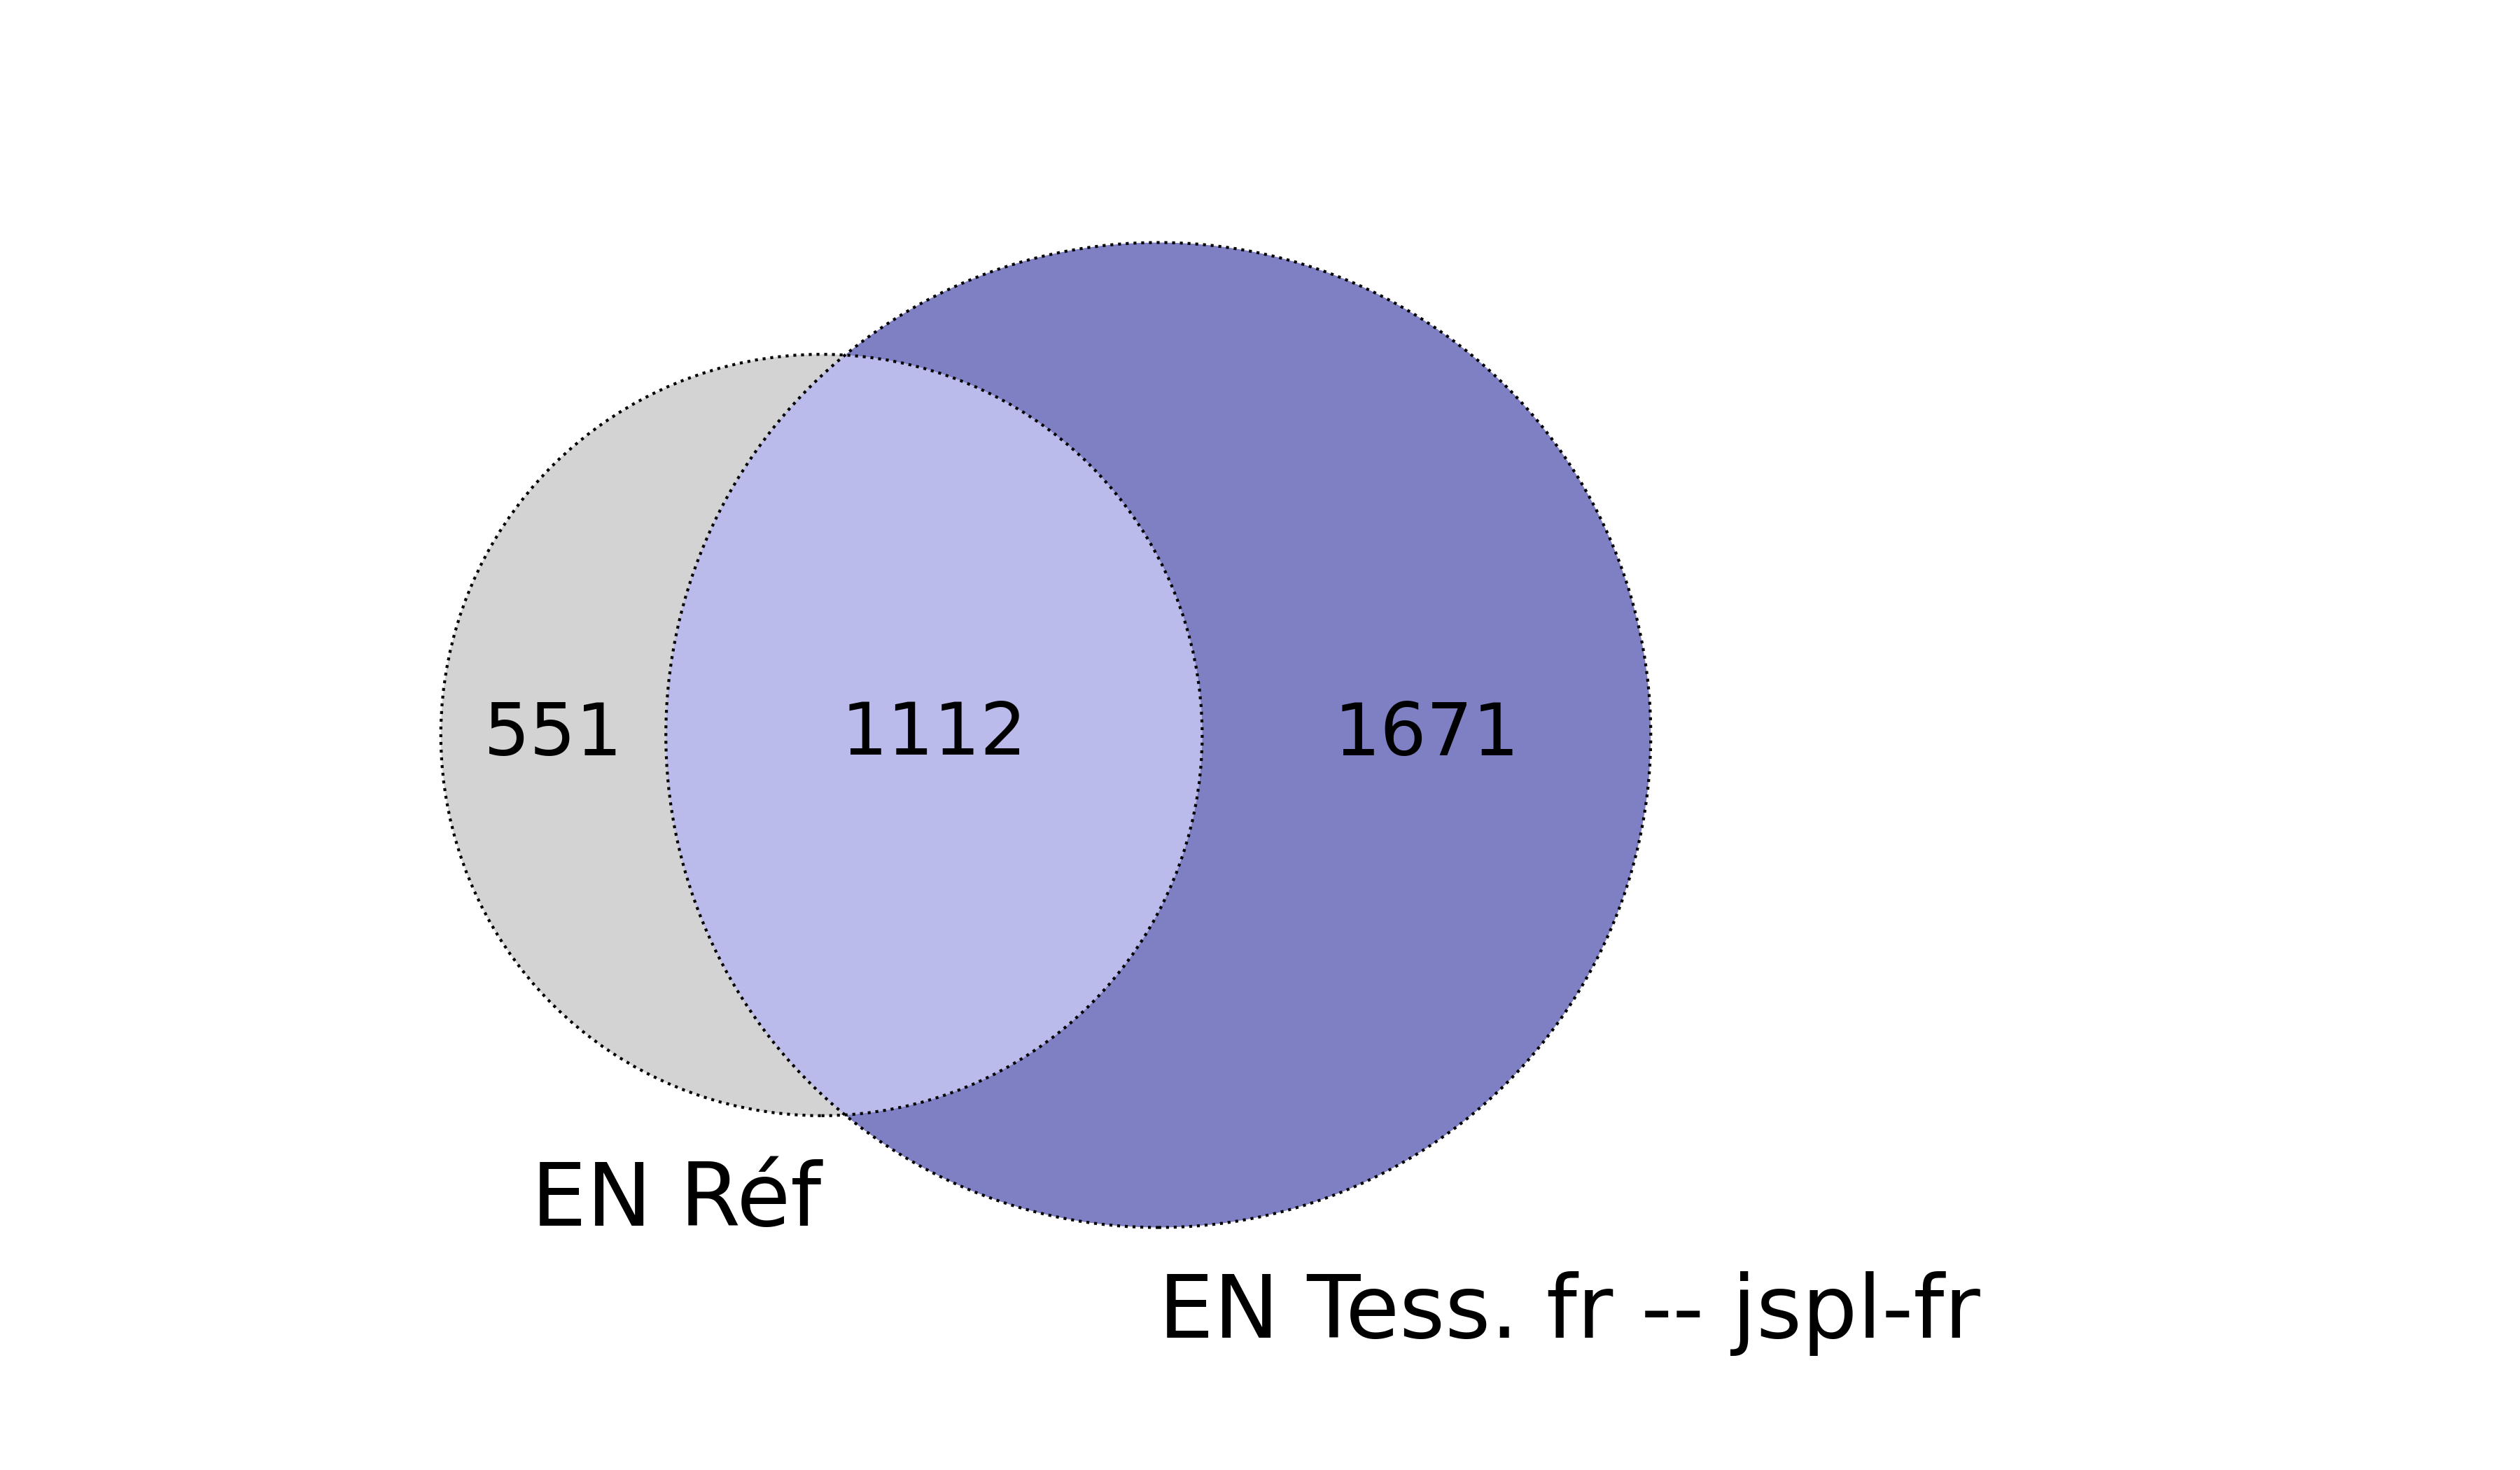
\includegraphics[width=1\textwidth]{IMAGES/INTERSECTIONS_GLOBALES/ELTeCFRA_Tess. fr -- jspl-fr_stanza-concat_intersection.png}
%  \caption{Tess. fr. corrigé -- \texttt{stanza}}
%  \label{fig:ELTeCFRA_Tess. fr -- jspl-fr_stanza-concat_intersection}
%  \end{subfigure}
%    \end{minipage}
%\caption{Intersections pour la configuration Tess-\texttt{spaCy\_lg} corrigées avec le modèle pré-entrainer de JamSpell et le modèle ELTeC, pour le sous-corpus ELTeC français.}
%\label{fig:intersection-globale-tess}
%\end{figure}

Lors du calcul de l'intersection entre les ensembles des EN de référence et des EN issues de ROC, nous rencontrons des problèmes d'alignement. L'alignement strict de l'EN de réf. \textit{Ormeaux} avec l'EN contaminée \textit{Ormaeuux} par la machine n'est pas possible et ce dernier est compté comme FP et ajouté à la liste des hapax, ce qui vient gonfler artificiellement le nombre des FP dans l'ensemble des EN de la ROC. Il s'agit en fait de Faux FP. Enfin, dans l'ensemble des EN reconnues sur les versions de ROC nous remarquons que la majorité des EN présentes dans les résultats obtenus sur la ROC sont effectivement présentes dans les résultats obtenus sur les versions de référence, comme le présente le tableau \ref{tab:FP_VP}. Il n'y a donc pas de véritable déperdition des VP. Enfin, il peut arriver plus rarement que des entités ne soient pas détectées sur la version de Réf. mais le soient sur la version de ROC. Il ne s'agit pas véritablement de FP, mais d'une erreur du système même en contexte non bruité.



En regard des différentes observations que nous venons d'apporter et parce que nous souhaitons rendre compte de la complexité de ces cas réels, nous proposons d'établir une typologie pour l'évaluation des contaminations de ROC sur la REN, élargissant la classification standard des vrais/faux positifs/négatifs. Si les FP sont qualifiés de bruit et les FN de silence, nous avons repéré qu'il existe différents types de bruit et de silence. %Cette typologie permet d'établir quels sont les vrais bruits autrement dit les Vrai FP et les vrais silences (Vrai VN). 


\begin{itemize}


	\item[] \textsc{Cas attendus}
	
	
	\begin{description}

		\item[Vrais positifs (VP)]: EN détectées dans les deux versions.
		\item[Vrais négatifs (VN)]: Aucune EN à reconnaître dans les deux versions.
		\item[Faux positif (FP)]: EN détectées à tort dans la version de ROC (bruit de la REN).
		\item[Faux négatif (FN)]: EN manquantes dans la version de ROC (silence de la REN).
	\end{description}
	
		
	\item[] \textsc{Sous évaluation du bruit et du silence de la REN}
	
	
	\begin{description}
	
		\item[Faux vrais positifs (FVP)]: EN détectées à tort dans les deux versions.
	
	 	\item[Faux vrais négatifs (FVN)] : EN manquantes dans les deux versions.
	 \end{description}
	 
	 \item[] \textsc{sur évaluation du bruit et du silence de la REN}
	
	\begin{description}
	
		\item[Faux faux positifs (FFP)]: EN détectées dans les versions de ROC mais pas dans le texte de référence (EN manquantes dans la référence$^{(i)}$ ou EN contaminées détectées dans la version de ROC$^{(ii)}$).
		
 		\item[Faux faux négatifs (FFN)]: EN  détectées à tort dans le texte de référence.

	\end{description}

\end{itemize}

%\begin{description}
%
%  \item[Vrais vrais positifs VP (VVP)]: EN correctement détectées dans les deux versions.
%  
%  %\item[Vrais vrais négatifs VN (VVN)]: Aucune EN n'est détectée par le système dans aucune version du texte, car il n'y en a pas.
%
%  \item[Vrais faux positifs FP (VFP)]: VRAI BRUIT EN détectées  à tort dans la version de ROC
%
%  \item[Vrais faux négatifs FN (VFN)]:  SILENCE EN détectées dans le texte de référence mais non détecté à tort dans la version de ROC.

%__________________________


%  \item[Faux vrais positifs (FVP)]:  BRUIT EN incorrectement détectées dans les deux versions.

%  \item[Faux vrais négatifs (FVN)] :  Silence total EN manquantes à tort dans les deux versions du texte.
%  

%  
%  \item[Faux faux négatifs (FFN)]: FAUX SILENCE EN  détectées à tort dans le texte de référence mais pas dans les versions de ROC.
%  

%    \item[Faux faux positifs (FFP)]: FAUX BRUIT EN détectées à raison dans les versions de ROC mais non détectées dans le texte de référence (silence dans la référence ou EN contaminées détectées dans la version de ROC).
%
%    
%\end{description}

Il existe un dernier cas des EN qui n'ont pas été transcrites par l'outil de ROC mais qui sont dans la Réf. Cette dernière catégorie est problématique car il ne s'agit pas véritable d'un FN de l'outil de REN, mais d'un FN de l'outil de ROC. 

Le cas de la version Kraken de Reynolds mets en exergue cette observation. Nous avons constaté que seuls 111 types d'EN ont été récupérés dans la configuration Kraken-\texttt{spaCy\_lg}, et pour cause plus de 90\% des pages du PDF n'ont pas été OCRisées très probablement à cause du flou très visible sur les pages concernées. D'autres PDF ont connu le même sort dans de très moindre proportions. De ce fait, une partie des entités manquantes dans les différentes configurations étudiées peuvent être dues non pas à la REN à proprement parler, mais à des transcriptions incomplètes. Nous n'avons pas mesuré l'impact de cette non transcription car il nous est apparu qu'elle était en faible proportion sur tout le corpus et le texte Reynolds était le seul cas très problématique. 


\begin{table}[h!]
    \centering
    %%%%%%%%%% Nouveau tableau sans stanza %%%%%%%%%%%%%%%%

\scriptsize{
\begin{tabular}{|l|l|l|l|}
%p{0.5cm}
\hline
% & \multicolumn{4}{c|}{TGB}\\\cline{2-5}
Type &Version & Contexte & \texttt{spaCy\_lg} \\
\hline
\hline
FVP&Réf. &\textit{[...] better than the milk-and-water lagrime}& lagrime\\
&Kraken &\textit{[...] better than the \textcolor{red}{\_}ilk-
and-water lagrime}& lagrime \\
\hline
FVN&Réf. & \textit{[...] l'été dans leur \textbf{propriété des Peuples}}& \textcolor{red}{()} \\
&Kraken &\textit{[...] l'ete dans leur \textbf{pro-
priete des Peuples}}& \textcolor{red}{()} \\
\hline
\hline
FFP &Réf. &\textit{[...] a sua entrada para o \textbf{colegio militar}}& \textcolor{red}{()} \\
&Kraken &\textit{[...] a s\textcolor{red}{\_}a entrada para
o col\textcolor{red}{c}gio milita}& col\textcolor{red}{c}gio milita \\
FFP &Réf. & \textit{[...] e na vespera delle ir para Coimbra}
&Coimbra \\
&Kraken & \textit{[...] e na vespera delle ir para Coim\textcolor{red}{h}ra} &Coim\textcolor{red}{h}ra \\
\hline
FFN&Réf. & \textit{[...] fleurs emblématiques que les \textcolor{red}{Bachagas}}& \textcolor{red}{Bachagas} \\
&Kraken & \textit{[...] fleurs embl\textcolor{red}{e-}
matiques que les Bach'agas}& () \\
\hline
\end{tabular}}
%\textcolor{red}{} 

%%%%%%%%%% Ancien tableau avec stanza 07/02/2024 %%%%%%%%%%%

%\scriptsize{
%\begin{tabular}{|l|l|l|l|l|}
%%p{0.5cm}
%\hline
%% & \multicolumn{4}{c|}{TGB}\\\cline{2-5}
%Type &Version & Contexte & \texttt{spaCy-lg} &\texttt{stanza}\\
%\hline
%\hline
%FVP&Réf. &\textit{[...] better than the milk-and-water}& lagrime  & ()\\
%&Kraken &\textit{[...] better than the \textcolor{red}{\_}ilk-
%and-water}& lagrime  & () \\
%\hline
%FVN&Réf. & \textit{[...] l'été dans leur \textbf{propriété des Peuples}}& \textcolor{red}{()}  &\textcolor{red}{()} \\
%&Kraken &\textit{[...] l'ete dans leur \textbf{pro-
%priete des Peuples}}& \textcolor{red}{()}  & \textcolor{red}{()}\\
%\hline
%\hline
%FFP $^{(i)}$&Réf. &\textit{[...] a sua entrada para o \textbf{colegio militar}}& \textcolor{red}{()}  & N/A\\
%&Kraken &\textit{[...] a s\textcolor{red}{\_}a entrada para
%o }& col\textcolor{red}{c}gio milita  &N/A \\
%FFP $^{(ii)}$&Réf. & \textit{[...] e na vespera delle ir para}
%&Coimbra& N/A\\
%&Kraken & \textit{[...] e na vespera delle ir para} &Coim\textcolor{red}{h}ra& N/A\\
%\hline
%FFN&Réf. & \textit{[...] fleurs emblématiques que les }& \textcolor{red}{Bachagas} &() \\
%&Kraken & \textit{[...] fleurs embl\textcolor{red}{e-}
%matiques que les Bach'agas}& () &() \\
%\hline
%\end{tabular}}
%%\textcolor{red}{} 

    \caption{Exemples pour la typologie d'évaluation de l'impact des erreurs de ROC sur la REN.}
    \label{tab:typo_eval}
\end{table}

%%%% Matrice mise de côté pour le moment
%En regard des différentes sorties de REN obtenues avec \texttt{spaCy} et \texttt{stanza}, nous proposons une typologie des contaminations de ROC, en élargissant la classification standard des vrais/faux positifs/négatifs. Les définitions correspondant à chaque catégorie (indiquées dans la matrice de confusion, tableau \ref{tab:Matrice_erreur_OCR_V2}) sont les suivantes :
%\begin{table}[H]
 %   \centering
  %  \begin{tabular}{|l|l|l|l|l|}
\hline
EN dans Réf.\ & EN dans la ROC & Éval.$_1$ & Description &  Éval.$_2$ \\
\hline
Oui      & Oui & VP    & Vrai VP & VVP \\ 
\hline
Oui      & Oui & VP    & Bruit dans les deux versions & FVP \\ 
\hline
\hline
%Non        & Non       & VN    & Silence dans les deux versions &  FVN \\
Non        & Non       & VN    & Silence dans les deux versions   & FVN\\ 
\hline
\hline
Oui     & Non         & FN    & Silence dans la ROC & VFN \\ 
\hline
Oui     & Non         & FN    &  Bruit dans la Réf.\ & FFN \\ 
\hline
\hline
Non       & Oui        & FP     &  Bruit dans la ROC & VFP \\
\hline
Non       & Oui        & FP     &  Silence dans la Réf.\ & FFP (VP) \\
\hline
Non       & Oui        & FP     &  Problème de liage d'EN & FFP (VP ?)\\
\hline
\end{tabular}

%%% version anglaise

% \begin{tabular}{|l|l|l|l|l|}
% \hline
% NER in Ref. & NER in OCR & Verdict 1 & Details &  Verdict 2 \\
% \hline
% Yes      & Yes & TP    & True Named Entity & True TP \\ 
% \hline
% Yes      & Yes & TP    & NER Error in Ref. and OCR & False TP  \\ 
% \hline
% \hline
% No        & No       & TN    & No entity in any version   & True TN\\ 
% \hline
% No        & No       & TN    & Missing entity in both versions &  False TN \\ 
% \hline
% \hline
% Yes     & No         & FN    & Missing entity in OCR & True FN \\ 
% \hline
% Yes     & No         & FN    &  Entity error in ref. & False FN \\ 
% \hline
% \hline
% No       & Yes        & FP     &  Entity error in OCR & True FP \\
% \hline
% No       & Yes        & FP     &  Missing entity in Ref. & False FP (TP) \\
% \hline
% No       & Yes        & FP     &  Entity linking issue & False FP (TP ?)\\
% \hline
% \end{tabular}
   % \caption{Typologie des contaminations d'OCR étendue.}
    %\label{tab:my_label}
%\end{table}



%\begin{table}[h!]
%    \centering
%    \scriptsize{\begin{tabular}{|ll|llll|}
\hline
\multicolumn{2}{|l|}{}                                            & \multicolumn{4}{l|}{Réf.}                              \\ 
\cline{3-6} 
\multicolumn{2}{|l|}{\multirow{-2}{*}{}}                    & \multicolumn{1}{l|}{IN}
    & \multicolumn{1}{l|}{\sout{IN}}          
    & \multicolumn{1}{l|}{\sout{OUT}}   
    & \multicolumn{1}{l|}{OUT}      \\ 
\hline
\multicolumn{1}{|l|}{}                      
    & IN                         
    & \multicolumn{1}{l|}{VVP}
    & \multicolumn{1}{l|}{\cellcolor[HTML]{000000}} 
    & FFP   
    %& \multicolumn{1}{l|}{\textcolor{blue}{VFP}}
    & \multicolumn{1}{l|}{\cellcolor[HTML]{000000}}\\ 
\cline{2-6} 
\multicolumn{1}{|l|}{}                      
    & \sout{IN}             
    & \multicolumn{1}{l|}{\cellcolor[HTML]{000000}}  
    & \multicolumn{1}{l|}{FVP}                      
    & \cellcolor[HTML]{000000} 
    & \multicolumn{1}{l|}{VFP}\\ 
\cline{2-6}
\multicolumn{1}{|l|}{\multirow{-4}{*}{ROC}} 
    & \sout{OUT}           
    & \multicolumn{1}{l|}{VFN} 
    & \multicolumn{1}{l|}{\cellcolor[HTML]{000000}} 
    & FVN  
    & \multicolumn{1}{l|}{\cellcolor[HTML]{000000}}                    \\ 
%\hline
\cline{2-6} 
\multicolumn{1}{|l|}{}                      & {\color[HTML]{000000} OUT} 
    %& \multicolumn{1}{l|}{\textcolor{blue}{FN}} 
    & \multicolumn{1}{l|}{\cellcolor[HTML]{000000}}
    & \multicolumn{1}{l|}{FFN} 
    & \cellcolor[HTML]{000000} 
    & \multicolumn{1}{l|}{VVN}\\
\hline
\end{tabular}}

%
%    \caption{Matrice de confusion pour l'évaluation de la REN sur des sorties ROC bruitées. IN = correctement détecté ; \sout{IN} = incorrectement détecté ; OUT = correctement ignoré ; \sout{OUT} = oublié ; case noire = cas impossible}
%    \label{tab:Matrice_erreur_OCR_V2}
%\end{table}

%\begin{table}[]
 %   \centering
  %  \begin{tabular}{|ll|llll|}
\hline
\multicolumn{2}{|l|}{}                                                   & \multicolumn{4}{l|}{Réf.}                                                                                                                                                \\ \cline{3-6} 
\multicolumn{2}{|l|}{\multirow{-2}{*}{}}                                 & \multicolumn{1}{l|}{IN}                       & \multicolumn{1}{l|}{OUT}                      & \multicolumn{1}{l|}{\sout{IN}}          & \sout{OUT}         \\ \hline
\multicolumn{1}{|l|}{}                      & IN                         & \multicolumn{1}{l|}{VP}                       & \multicolumn{1}{l|}{FP}                       & \multicolumn{1}{l|}{\cellcolor[HTML]{000000}} & FFP                      \\ \cline{2-6} 
\multicolumn{1}{|l|}{}                      & {\color[HTML]{000000} OUT} & \multicolumn{1}{l|}{FN}                       & \multicolumn{1}{l|}{VN}                       & \multicolumn{1}{l|}{FFN}                      & \cellcolor[HTML]{000000} \\ \cline{2-6} 
\multicolumn{1}{|l|}{}                      & \sout{IN}             & \multicolumn{1}{l|}{\cellcolor[HTML]{000000}} & \multicolumn{1}{l|}{VFP}                      & \multicolumn{1}{l|}{FVP}                      & \cellcolor[HTML]{000000} \\ \cline{2-6} 
\multicolumn{1}{|l|}{\multirow{-4}{*}{ROC}} & \sout{OUT}           & \multicolumn{1}{l|}{VFP}                      & \multicolumn{1}{l|}{\cellcolor[HTML]{000000}} & \multicolumn{1}{l|}{\cellcolor[HTML]{000000}} & FVN                      \\ \hline
\end{tabular}

   % \caption{Matrice de confusion pour l'évaluation de la REN sur des sorties ROC bruitées. IN = correctement détecté ; \sout{IN} = incorrectement détecté ; OUT = correctement ignoré ; \sout{OUT} = oublié}
    %\label{tab:Matrice_erreur_OCR_V1}
%\end{table}

\subsection{\'Evaluation semi-supervisée des contaminations de ROC sur un corpus annoté}

Afin d'évaluer de manière plus supervisée l'influence du bruit ROC sur la REN nous avons annoté un échantillon du sous-corpus ELTeC français.
 Nous avons choisi de nous limiter aux quatre catégories présentes dans Spacy (Lieux, Personnes, Organisations et Divers).
  Nous avons tout d'abord annoté un échantillon de 3~000 tokens d'une œuvre  puis réalisé une adjudication pour régler les désaccords. 
  Nous avons ensuite annoté 5 000 tokens de 3 versions (Référence, Tesseract et Kraken) de deux œuvres (Daudet et Maupassant)

L'accord inter-annotateur (Kappa de  Fleiss \cite{fleiss2013statistical}) était de $0.877$, significativement plus élevé sur la version de référence ($0.905$) que sur les versions ROC. Nous avons pu observer que les désaccords étaient plus nombreux sur l'annotation des versions océrisées du fait des problèmes de tokenisation.

Grâce à un système de vote majoritaire, nous avons fusionné les annotations pour obtenir un \textit{gold standard} sur chaque version de chaque œuvre.
 Nous avons évalué \texttt{spaCy\_lg} sur cet échantillon, les résultats sont présentés dans le tableau \ref{tab:eval-supervise}.
 En commençant par l'évaluation dite ``GLOBALE'' (tous les types d'entités) nous pouvons remarquer d'une part que les résultats obtenus sur les versions Tesseract sont meilleurs que ceux obtenus sur les versions Kraken. Mais aussi, et ce qui est plus étonnant, que pour ce qui est de l'évaluation souple (où une partie de l'entité suffit à considérer la réponse bonne), que ces résultats sont même meilleurs que ceux obtenus sur la version de référence.
  D'autre part, nous remarquons que là aussi la faiblesse apparente des résultats de REN obtenus sur des versions OCR est principalement due à des problèmes d'alignement entre les tokens contaminés et les tokens de référence. 
\begin{table}[h!]
\scriptsize{\begin{tabular}{l|ccc|ccc}
 %Versions
 &		&	GLOBAL	&		&		&	LIEUX	&		\\
\hline
 \hline
\textbf{Souple}	&	Rappel		&Précision	&	F-Mes.	&	Rappel&		Précision		&F-Mes.	\\
 \hline
Kraken	&	49.57	&	73.72 	&	59.28	&	48.84	&	52.50	&	50.60	\\
													
Tesseract	&	51.53	&	77.63	&	61.94	&	56.41	&	57.89	&	57.14	\\
													
Référence	&	49.78	&	77.55	&	60.64	&	53.49	&	53.49	&	53.49	\\
\hline
\hline
\textbf{Stricte}	&	Rappel		&Précision	&	F-Mes.	&	Rappel&		Précision		&F-Mes.	 \\
\hline
Kraken	&	18.26	&	58.82	&	27.87	&	43.24	&	45.71	&	44.44	\\
Tesseract	&	21.00	&	68.66	&	32.16	&	43.33	&	44.83	&	44.07	\\
Référence	&	21.62	&	69.57	&	32.98	&	41.18	&	45.16	&	43.08	\\
\hline
\hline
\end{tabular}}
\caption{Evaluation de \texttt{spaCy\_lg} sur un échantillon annoté de 10~000 tokens dans trois versions textuelles différentes\label{tab:eval-supervise} en configuration souple et en configuration stricte (GLOBAL: tous les types d'entités), LIEUX: seulement les lieux)}
 \end{table}






%--------------------Correction automatique

\section{Analyse de l'impact des corrections de ROC sur la REN}
\label{sec:COR-OCR-IMPACT-NER}
\textbf{Cette section présente l'outil JamSpell (Jspll) et les modèles de langue utilisés pour la correction automatique de ROC et la performance de cet outil. Nous réutilisons le même procédé d'évaluation des contaminations de corrections de ROC issues de l'analyse manuelle. Bien que nous ayons déterminé qu'il s'agit d'une manière trop stricte d'évaluer la REN en contexte bruité nous réemployons les intersections. Nous utilisons  des mesures de distance textuelle pour mener une évaluation plus souple. Enfin, nous calculons la précision, le rappel et le F-score à l'aide de l'outil \textsc{Nerval}.}

\subsection{Outils de la correction des sorties ROC utilisés dans le cadre de cette étude}
\label{subsec:outils_COR-OCR-IMPACT-NER}
\textbf{Concernant la correction automatique des textes issus des transcriptions ROC, nous avons utilisé Jspll, un outil développé en Python qui exploite un modèle de langue trigramme statistique\footnote{Pour plus de détails sur ce modèle \textit{cf}. \url{https://habr.com/en/articles/346618/}.} (grain mot), dont une partie des fonctionnalités est mise à disposition gratuitement sur le web.
% \footnote{Malgré de nombreuses tentatives d'installation sur nos machines en local, nous avons dû nous résoudre à le faire tourner dans un environnement Google Colab.}
Si les modèles de langues pour le français et l'anglais sont accessibles gratuitement, le modèle portugais est disponible uniquement dans la version payante de Jspll, de fait cette option n'a pas été testée.
Nous avons entraîné un modèle de langue pour Jspll pour chacune des trois langues. Pour ce faire, nous avons sélectionné 40\% de chacun des corpus mis à disposition par ELTeC\footnote{\textbf{soit 4 millions de tokens pour chaque modèle. A VERIFIER}} et nous en avons exclu les textes utilisés pour notre étude.}

\textbf{Nous avons donc procédé aux évaluations des différentes configurations présentées dans le tableau \ref{tab:config}}.

\begin{table}[h!]
    \centering
   %\scriptsize{\begin{tabular}{|c|cc|cc|cc|cc|}
%
%\hline   
%ROC &  \multicolumn{2}{l|}{Kraken} &  \multicolumn{2}{l|}{Tess. en} & \multicolumn{2}{l|}{Tess. fr} &  \multicolumn{2}{l|}{Tess. pt} \\ 
%\hline
%REN & \textit{sp}} & \textit{st} & \textit{sp}} & \textit{st}&\textit{sp}} & \textit{st} &\textit{sp}} & \textit{st} \\
%\hline
%non corr. &\ding{51}} & \ding{51} & \ding{51}} & \ding{51}&\ding{51}} & \ding{51} &\ding{51}} & \ding{53} \\
%Jspll-pretr. &\ding{51}} & \ding{51} & \ding{51}} & \ding{51}&\ding{51}} & \ding{51} &\ding{53}} & \ding{53} \\
%Jspll-ELTeC  &\ding{51}} & \ding{51} & \ding{51}} & \ding{51}&\ding{51}} & \ding{51} &\ding{51}} &\ding{53}  \\
%  \hline
%\end{tabular}}

% \begin{tabular}{|c|cccc|}
% \hline
% ROC          & \multicolumn{1}{l|}{Kraken}                 & \multicolumn{1}{l|}{Tess. en}               & \multicolumn{1}{l|}{Tess. fr}               & \multicolumn{1}{l|}{Tess. pt} \\ \hline
% REN          & \multicolumn{4}{c|}{\textbackslash{}textttspaCy\_lg}                                                                                                                    \\ \hline
% non corr.    & \multicolumn{1}{c|}{\textbackslash{}ding51} & \multicolumn{1}{c|}{\textbackslash{}ding51} & \multicolumn{1}{c|}{\textbackslash{}ding51} & \textbackslash{}ding51        \\
% Jspll-pretr. & \multicolumn{1}{c|}{\textbackslash{}ding51} & \multicolumn{1}{c|}{\textbackslash{}\ding51 & \multicolumn{1}{c|}{\textbackslash{}ding51} & \textbackslash{}ding53        \\
% Jspll-ELTeC  & \multicolumn{1}{c|}{\textbackslash{}ding51} & \multicolumn{1}{c|}{\textbackslash{}ding51} & \multicolumn{1}{c|}{\textbackslash{}ding51} & \textbackslash{}ding51        \\ \hline
% \end{tabular}



% \scriptsize{\begin{tabular}{|c|c|c|c|c|}

% \hline   
% ROC &  Kraken &  Tess. en & Tess. fr &  Tess. pt \\ 
% \hline
% REN & \multicolumn{2}{c|}{\texttt{spaCy\_lg}} &  &  & \\
% % \hline
% non corr. &\ding{51} & \ding{51} &\ding{51} &\ding{51} \\
% Jspll-pretr. &\ding{51} & \ding{51} &\ding{51}&\ding{53} \\
% Jspll-ELTeC  &\ding{51} & \ding{51} &\ding{51}  &\ding{51}  \\
%   \hline
% \end{tabular}}

\scriptsize{
\begin{tabular}{|c|cccc|}
\hline
ROC          & \multicolumn{1}{l|}{Kraken}                 & \multicolumn{1}{l|}{Tess.en}               & \multicolumn{1}{l|}{Tess.fr}               & \multicolumn{1}{l|}{Tess.pt} \\ \hline
REN          & \multicolumn{4}{c|}{\texttt{spaCy\_lg}}                                                                                                                    \\ \hline
non corr.    & \multicolumn{1}{c|}{\ding{51}} & \multicolumn{1}{c|}{\ding{51}} & \multicolumn{1}{c|}{\ding{51}} & \ding{51}        \\
Jspll-pretr. & \multicolumn{1}{c|}{\ding{51}} & \multicolumn{1}{c|}{\ding{51}} & \multicolumn{1}{c|}{\ding{51}} & \ding{53}        \\
Jspll-ELTeC  & \multicolumn{1}{c|}{\ding{51}} & \multicolumn{1}{c|}{\ding{51}} & \multicolumn{1}{c|}{\ding{51}} & \ding{51}        \\ \hline
\end{tabular}
}

    \caption{Ensemble des configurations que nous évaluons dans cette étude. \texttt{spaCy\_lg}: sp.}
    \label{tab:config}
\end{table}

\subsection{Typologie des contaminations de corrections de ROC issues de l'analyse manuelle}
\label{subsec:Typologie_COR-OCR-IMPACT-NER}

\textbf{En observant les exemples de correction de ROC présentés dans cette sous-section, nous constatons certaines fluctuations au niveau de la performance du correcteur automatique.}
Notons le cas particulier de l'EN ``Meunet-sur-Vatan'' dont les déclinaisons différentes en fonction du type de correcteur automatique sont indiquées dans le tableau \ref{tab:erreurs_corr_ELTeCFra}. Nous nous apercevons que les différentes versions de cette EN, contaminée par les différentes OCRisations et sur-corrections, n'ont pas du tout été extraites par \texttt{spaCy\_lg}.
%¨

\begin{table}[h!]
    \small
    \centering
   %%%%%%%%% Nouveau tableau sans stanza %%%%%%%%%%%


\begin{tabular}{|l|l|l|l|}

\hline

\bf{Version} & \bf {Contexte} & \bf{\texttt{spaCy\_lg}}\\
\hline 
Réf.\ & \textit{[\dots]  à l'assemblée de Meunet-sur-Vatan ;} & Meunet-sur-Vatan \\
 Kraken & \textit{[\dots]  \textcolor{red}{a} l'assem\textcolor{red}{h}l\textcolor{red}{6e'} de \textcolor{red}{N}eunet-sur-
\textcolor{red}{Y}atan'}& \textcolor{red}{Y}atan \\ 
 Kraken Jspll-fr &\textit{[\dots]  a l'assembl\textcolor{red}{6e'} de \textcolor{red}{N}eune\textcolor{red}{r}-sur-
\textcolor{red}{S}atan\textcolor{red}{'};}&\textcolor{red}{()} \\
  Kraken ELTeC-fr &\textit{[\dots]  a l'assem\textcolor{red}{h}l\textcolor{red}{6e'} de \textcolor{red}{N}eunet-sur-\textcolor{red}{Avant'};}&\textcolor{red}{()}\\


 %Tess & \textit{[\dots]  \textcolor{red}{4} l'assemblée\textcolor{red}{‘} de Meunet-sur-\textcolor{red}{y}Vatan\textcolor{red}{*}; } & \textcolor{red}{()} &Meunet-sur-\textcolor{red}{y}Vatan  \\
Tess fr &\textit{[\dots]  à l'assemblée\textcolor{red}{’} de Meunet-sur-\textcolor{red}{|} Vatan\textcolor{red}{*};  }& Meunet-sur-\textcolor{red}{|} \\
Tess fr Jspll-fr&\textit{[\dots]  à l'assemblée\textcolor{red}{’} de Meu\textcolor{red}{r}et-sur-
\textcolor{red}{|} Vatan\textcolor{red}{*};}&\textcolor{red}{()} \\
Tess fr ELTeC-fr& \textit{[\dots]  à l'assemblée\textcolor{red}{’} de Meunet-sur-\textcolor{red}{|} Vatan\textcolor{red}{*};}&Meunet-sur\textcolor{red}{\_}\\
\hline
\end{tabular}


%%%%%%%%% Ancien tableau avec stanza %%%%%%%%%%%%%

%\resizebox{\textwidth}{!}{
%\begin{tabular}{|l|l|l|l|l|l|}
%
%\hline
%
%\bf{Version} & \bf {Contexte} & \bf{\texttt{spaCy\_lg}}&\bf{\texttt{stanza}}\\
%\hline 
%Réf.\ & \textit{[\dots]  à l'assemblée de Meunet-sur-Vatan ;} & Meunet-sur-Vatan&Meunet-sur-Vatan \\
% Kraken & \textit{[\dots]  \textcolor{red}{a} l'assem\textcolor{red}{h}l\textcolor{red}{6e'} de \textcolor{red}{N}eunet-sur-
%\textcolor{red}{Y}atan'}& \textcolor{red}{Y}atan&\textcolor{red}{N}eunet-sur-
%\textcolor{red}{Y}atan \\ 
% Kraken Jspll-fr &\textit{[\dots]  a l'assembl\textcolor{red}{6e'} de \textcolor{red}{N}eune\textcolor{red}{r}-sur-
%\textcolor{red}{S}atan\textcolor{red}{'};}&\textcolor{red}{()}&\textcolor{red}{N}eune\textcolor{red}{r}-sur-
%\textcolor{red}{S}atan\\
%  Kraken ELTeC-fr &\textit{[\dots]  a l'assem\textcolor{red}{h}l\textcolor{red}{6e'} de \textcolor{red}{N}eunet-sur-\textcolor{red}{Avant'};}&\textcolor{red}{()}&\textcolor{red}{N}eunet-sur\textcolor{red}{\_}\\
%
%
% %Tess & \textit{[\dots]  \textcolor{red}{4} l'assemblée\textcolor{red}{‘} de Meunet-sur-\textcolor{red}{y}Vatan\textcolor{red}{*}; } & \textcolor{red}{()} &Meunet-sur-\textcolor{red}{y}Vatan  \\
%Tess fr &\textit{[\dots]  à l'assemblée\textcolor{red}{’} de Meunet-sur-\textcolor{red}{|} Vatan\textcolor{red}{*};  }& Meunet-sur-\textcolor{red}{|} &   Meunet-sur-\textcolor{red}{|} Vatan\\
%Tess fr Jspll-fr&\textit{[\dots]  à l'assemblée\textcolor{red}{’} de Meu\textcolor{red}{r}et-sur-
%\textcolor{red}{|} Vatan\textcolor{red}{*};}&\textcolor{red}{()}&Meu\textcolor{red}{r}et-sur-
%\textcolor{red}{|} Vatan\\
%Tess fr ELTeC-fr& \textit{[\dots]  à l'assemblée\textcolor{red}{’} de Meunet-sur-\textcolor{red}{|} Vatan\textcolor{red}{*};}&Meunet-sur\textcolor{red}{\_}&Meunet-sur-\textcolor{red}{|} Vatan\\
%\hline
%\end{tabular}
%}
     \caption{Exemples illustrant l'impact de la correction de ROC sur la REN avec \texttt{spaCy\_lg}. {\normalfont La petite Jeanne}, Carraud.}
    \label{tab:erreurs_corr_ELTeCFra}
\end{table}

De façon similaire, nous observons dans le tableau \ref{tab:erreurs_corr_ELTeCEng} que le modèle de la correction automatique de ROC par Jspll, entraîné sur le corpus ELTeC, n'a pas eu d'impact sur l'extraction de l'EN ``Iudia'', puisqu'elle n'avait pas été corrigée en l'EN de référence ``India''. Par contre, le modèle Jspll pré-entraîné a bien corrigé la même EN, ce qui a permis son extraction sous forme correcte.
\begin{table}[h!]
\small
    \centering
   %%%%%%%%%%% Nouveau tableau sans stanza %%%%%%%%%%%

\begin{tabular}{|l|l|l|}

\hline

\bf{Version} & \bf {Contexte} & \bf{\texttt{spaCy\_lg}} \\
\hline 
Réf.\ &\textit{[...] before you went to India.} &India \\
 Kraken &\textit{[...] before you went to I\textcolor{red}{u}dia.}&I\textcolor{red}{u}dia \\ 
 Kraken Jspll-en &\textit{[...] before you went to India}&India \\ 
 Kraken ELTeC-en &\textit{[...] before you went to I\textcolor{red}{u}dia.}&I\textcolor{red}{u}dia \\ 
% Tess &\textit{[...] before you went to India.}&India& India\\
 % Tess jspl &\textit{[...] before you went to India.}&India& India\\
  % Tess ELTeC &\textit{[...] before you went to India.}&India& India\\

\hline
\end{tabular}


%%%%%%%% Ancien tableau avec stanza %%%%%%%%%%%

%\begin{tabular}{|l|l|l|l|l|l|}
%
%\hline
%
%\bf{Version} & \bf {Contexte} & \bf{\texttt{spaCy\_lg}}&\bf{\texttt{stanza}}\\
%\hline 
%Réf.\ &\textit{[...] before you went to India.} &India &India \\
% Kraken &\textit{[...] before you went to I\textcolor{red}{u}dia.}&I\textcolor{red}{u}dia&I\textcolor{red}{u}dia\\ 
% Kraken Jspll &\textit{[...] before you went to India}&India &India\\ 
% Kraken ELTeC &\textit{[...] before you went to I\textcolor{red}{u}dia.}&I\textcolor{red}{u}dia&I\textcolor{red}{u}dia\\ 
%% Tess &\textit{[...] before you went to India.}&India& India\\
% % Tess jspl &\textit{[...] before you went to India.}&India& India\\
%  % Tess ELTeC &\textit{[...] before you went to India.}&India& India\\
%
%\hline
%\end{tabular}

    \caption{Exemples illustrant l'impact de la correction de ROC sur la REN avec \texttt{spaCy\_lg}. {\normalfont Vanity Fair}, Thackeray.}
    \label{tab:erreurs_corr_ELTeCEng}
\end{table}

%\begin{table}
%\small
 %   \centering
  % \begin{tabular}{|l|p{4cm}|l|l|l|}
%p{0.5cm}
\hline
\bf{Version} & \bf {Contexte} & \bf{\texttt{spaCy\_lg}}&\bf{\texttt{stanza}}\\
\hline
Réf.\ & \textit{Alegre Inglaterra! oh! alegre Inglaterra!} &Alegre Inglaterra &  N/A\\
&  &Inglaterra &  N/A\\
\hline
 Kraken &\textit{Alegre Inglate\textcolor{red}{n- }ra\textcolor{red}{l} oh\textcolor{red}{l} alegre Inglat\textcolor{red}{l}erra\textcolor{red}{.l}} &Alegre Inglate\textcolor{red}{n-} &  N/A\\
& &\textcolor{red}{()}&  N/A\\ 
\hline
Kraken ELTeCpt  &\textit{Alegre Inglate\textcolor{red}{n- }ra\textcolor{red}{l} oh\textcolor{red}{l} alegre Inglat\textcolor{red}{l}erra\textcolor{red}{.l}} &Alegre Inglate\textcolor{red}{n-}   & N/A \\
& &  \textcolor{red}{()}& N/A \\
\hline
Tess pt  &\textit{Alegre Inglater\textcolor{red}{-} ra\textcolor{red}{l} oh! alegre Inglaterra!} & Alegre Inglater\textcolor{red}{-} ra\textcolor{red}{l} oh! & N/A \\
& & Inglaterra & N/A \\
\hline
Tess pt ELTeCpt  & \textit{Alegre \textcolor{red}{Singular-} ral oh! alegre Inglaterra!}&Alegre \textcolor{red}{Singular-} ral oh!&N/A\\
& & Inglaterra & N/A \\

\hline
\end{tabular}


   % \caption{Exemples illustrant l'impact de la correction de ROC sur la REN avec \texttt{spaCy\_lg} et \texttt{stanza}, {\normalfont Uma familia ingleza}, Diniz.}
    %\label{tab:erreurs_corr_ELTeCPor}
%\end{table}

\textbf{À partir des exemples présentés dans les tableaux \ref{tab:erreurs_corr_ELTeCFra} et \ref{tab:erreurs_corr_ELTeCEng}, nous pouvons dériver une typologie des corrections automatiques de ROC, résumée dans le tableau \ref{tab:res-analyses}. Cela permet de distinguer les différents cas de figure où les corrections en question ont soit amélioré les sorties de ROC (MOBC), soit les ont incorrectement modifiées (MOMC, BOIC) ou même ignorées (MOI).}
%Nous nous appuyons également sur une typologie des corrections automatiques de ROC, résumée dans le tableau \ref{tab:res-analyses}, qui permet de distinguer les différents cas de figure où les corrections en question ont soit amélioré les sorties de ROC (MOBC), soit les ont incorrectement modifiées (MOMC, MOI, BOIC). 

\begin{table}[h!]
\small
    \centering
    \begin{tabular}{|l|l|}
%p{0.5cm}
\hline
 
Type Acronyme& Définition\\
\hline
MOBC & mal océrisées bien corrigées\\

\hline
MOMC& mal océrisées mal corrigées\\

\hline
MOI&mal océrisées ignorées \\
\hline
BOIC&  bien océrisées indûment corrigées \\
\hline
\end{tabular}



    \caption{Typologie de l'impact de la correction de ROC sur la REN.  }
    \label{tab:res-analyses}
\end{table}

\textbf{Pour illustrer ce propos, q}uelques exemples sont \textbf{indiqués} dans le tableau \ref{tab:typologie_erreurs-corr_ELTeCEng}, 
% et \ref{tab:typologie_erreurs_corr_ELTeCFra}
parmi lesquels se distinguent les sur-corrections ``Conspire'' 
% et ``Earlier'' 
(au lieu de ``Devonshire'' 
% et ``Algiers''
dans ELTeC anglais), ainsi que ``Martincourt'' (au lieu de ``Morlincourt'' dans ELTeC français).

\begin{table}[h!]
\small
    \centering
   %%%%%%%%%%%% Nouveau tableau sans stanza %%%%%%%%%%%%%%

\resizebox{\textwidth}{!}{
\begin{tabular}{|l|l|l|l|}
%p{0.5cm}
\hline
% & \multicolumn{4}{c|}{TGB}\\\cline{2-5}
Type &Version & Contexte & \texttt{spaCy\_lg} \\
\hline
MOBC &Kraken &\textit{[…] when they were in Lon\textcolor{red}{l}on}&() \\
&Jspll&\textit{[…] when they were in London}&London \\
&ELTeC&\textit{[…] when they were in London}&London \\
\hline
MOMC& Kraken&\textit{[…] flowery
lanes peeuliar to \textcolor{red}{Dc}onshire;}&\textcolor{red}{Dc}onshire \\
&Jspll&\textit{[…] flowery
lanes peculiar to \textcolor{red}{Conspire};}&() \\
&ELTeC&\textit{[…] flowers
lanes peculiar to \textcolor{red}{Dc}onshire;}&\textcolor{red}{Dc}onshire \\
\hline
% MOI&Kraken&\textit{ […] dark woo\textcolor{red}{l} within
% ten miles of Oakwoo\textcolor{red}{l}.}& Oakwoo\textcolor{red}{l} &Oakwoo\textcolor{red}{l}\\
% &Jspll&\textit{[…] dark woo\textcolor{red}{l} within
% ten miles of Oakwoo\textcolor{red}{l}.}&  Oakwoo\textcolor{red}{l}&Oakwoo\textcolor{red}{l}\\
% &ELTeC&\textit{ […] dark wool within
% ten miles of Oakwoo\textcolor{red}{l}.}& Oakwoo\textcolor{red}{l}&Oakwoo\textcolor{red}{l}\\
% \hline
% BOIC&Kraken&\textit{[…] which the bombardment of Algiers } &Algiers&Algiers\\
% &Jspll&\textit{[…] which the bombardment of Algiers}&Algiers&Algiers\\
% &ELTeC&\textit{[…] which the bombardment of\textbf{ Earlier}}&\textcolor{red}{()}&\textcolor{red}{()}\\
% \hline
MOI&Kraken& \textit{cure de M\textcolor{red}{l}orlincourt\textcolor{red}{l}}& M\textcolor{red}{l}orlincourt\textcolor{red}{l} \\
&Jspll-fr&\textit{cure de  M\textcolor{red}{l}orlincourt\textcolor{red}{l}} &   M\textcolor{red}{l}orlincourt\textcolor{red}{l} \\
&ELTeC-fr& \textit{cure de  M\textcolor{red}{l}orlincourt\textcolor{red}{l}}&  M\textcolor{red}{l}orlincourt\textcolor{red}{l} \\
\hline
BOIC&Kraken& \textit{en retournant
de Morlincourt} &Morlincourt \\
&Jspll-fr&\textit{en retournant
de\textbf{ Martincourt}} & \textbf{Martincourt} \\
&ELTeC-fr&\textit{en retournant
de Morlincourt} &Morlincourt \\
\hline
\end{tabular}
%\label{tab:typologie_erreurs-corr_ELTeCEng}
}

%%%%%%%%%%%%%% Ancien tableau avec stanza %%%%%%%%%%%%%%%%%

%\resizebox{\textwidth}{!}{
%\begin{tabular}{|l|l|l|l|l|}
%%p{0.5cm}
%\hline
%% & \multicolumn{4}{c|}{TGB}\\\cline{2-5}
%Type &Version & Contexte & \texttt{spaCy\_lg} &\texttt{stanza}\\
%\hline
%MOBC &Kraken &\textit{[…] when they were in Lon\textcolor{red}{l}on}&()&Lon\textcolor{red}{l}on\\
%&Jspll&\textit{[…] when they were in London}&London&London\\
%&ELTeC&\textit{[…] when they were in London}&London&London\\
%\hline
%MOMC& Kraken&\textit{[…] flowery
%lanes peeuliar to \textcolor{red}{Dc}onshire;}&\textcolor{red}{Dc}onshire&\textcolor{red}{Dc}onshire\\
%&Jspll&\textit{[…] flowery
%lanes peculiar to \textcolor{red}{Conspire};}&()&\textcolor{red}{Conspire}\\
%&ELTeC&\textit{[…] flowers
%lanes peculiar to \textcolor{red}{Dc}onshire;}&\textcolor{red}{Dc}onshire&\textcolor{red}{Dc}onshire\\
%\hline
%% MOI&Kraken&\textit{ […] dark woo\textcolor{red}{l} within
%% ten miles of Oakwoo\textcolor{red}{l}.}& Oakwoo\textcolor{red}{l} &Oakwoo\textcolor{red}{l}\\
%% &Jspll&\textit{[…] dark woo\textcolor{red}{l} within
%% ten miles of Oakwoo\textcolor{red}{l}.}&  Oakwoo\textcolor{red}{l}&Oakwoo\textcolor{red}{l}\\
%% &ELTeC&\textit{ […] dark wool within
%% ten miles of Oakwoo\textcolor{red}{l}.}& Oakwoo\textcolor{red}{l}&Oakwoo\textcolor{red}{l}\\
%% \hline
%% BOIC&Kraken&\textit{[…] which the bombardment of Algiers } &Algiers&Algiers\\
%% &Jspll&\textit{[…] which the bombardment of Algiers}&Algiers&Algiers\\
%% &ELTeC&\textit{[…] which the bombardment of\textbf{ Earlier}}&\textcolor{red}{()}&\textcolor{red}{()}\\
%% \hline
%MOI&Kraken& \textit{cure de M\textcolor{red}{l}orlincourt\textcolor{red}{l}}& M\textcolor{red}{l}orlincourt\textcolor{red}{l} & M\textcolor{red}{l}orlincourt\textcolor{red}{l}\\
%&Jspll-fr&\textit{cure de  M\textcolor{red}{l}orlincourt\textcolor{red}{l}} &   M\textcolor{red}{l}orlincourt\textcolor{red}{l}& M\textcolor{red}{l}orlincourt\textcolor{red}{l}\\
%&ELTeC-fr& \textit{cure de  M\textcolor{red}{l}orlincourt\textcolor{red}{l}}&  M\textcolor{red}{l}orlincourt\textcolor{red}{l}&  M\textcolor{red}{l}orlincourt\textcolor{red}{l} \\
%\hline
%BOIC&Kraken& \textit{en retournant
%de Morlincourt} &Morlincourt &Morlincourt \\
%&Jspll-fr&\textit{en retournant
%de\textbf{ Martincourt}} & \textbf{Martincourt} & \textbf{Martincourt} \\
%&ELTeC-fr&\textit{en retournant
%de Morlincourt} &Morlincourt &Morlincourt \\
%\hline
%\end{tabular}
%%\label{tab:typologie_erreurs-corr_ELTeCEng}
%}

%\begin{tabular}{|l|l|l|l|l|}
%p{0.5cm}
%\hline
 %& \multicolumn{4}{c|}{TGB}\\\cline{2-5}
%&OCR & Corr. & REN &REN corr.\\
%\hline
%MOBC &“[…] Sainl-Cyr”&“[…] Saint-Cyr”&Sainl-Cyr&Saint-Cyr\\

%\hline
%MOMC& “[…] Nîme”&“[…] Mîme”&Nîme&Mîme\\

%\hline
 %MOI& 
%“[…] SaintAntoine”&
%“[…] SaintAntoine”&
%SaintAntoine &
 %SaintAntoine\\
%\hline
%BOIC&  
%“[…] Pinde”&
%“[…] Inde”&
%Pinde&
%Et du sommet du Inde\\
%\hline
%\end{tabular}
    \caption{Exemples illustrant la typologie de l'impact de la correction de ROC sur la REN avec \texttt{spaCy\_lg}. Configuration : Jspll -- correction avec le modèle pré-entraîné de JamSpell, ELTeC -- correction avec le modèle entraîné sur une partie de chaque corpus ELTeC. Formes de références des entités : London, Devonshire, Morlincourt. {\normalfont Home influence}, Aguillar et {\normalfont Mon village}, Adam.}
    \label{tab:typologie_erreurs-corr_ELTeCEng}
\end{table}

% Le MOI et BOIC de ce tableau a été déplacé dans le tableau 13 (on a fusionné les deux tableaux, donc on a le MOBC et le MOMC du tableau 13 et le MOI et le BOIC du tableau 14)

% \begin{table}[h!]
% \small
%     \centering
%    \begin{tabular}{|l|l|l|l|l|}
%p{0.5cm}
\hline
% & \multicolumn{4}{c|}{TGB}\\\cline{2-5}
Type &Version & Contexte & \texttt{spaCy-lg} &\texttt{stanza}\\
\hline
MOBC &Kraken &\textit{[…] ville que ce Paris\textcolor{red}{l} Ici}& Paris\textcolor{red}{l} Ici & () \\
&Jspll&\textit{[…] ville que ce \textbf{Paris} Ici}& Paris &Paris \\
&ELTeC&\textit{[…] ville que ce Paris\textcolor{red}{l} Ici} & Paris\textcolor{red}{l} Ici &() \\
\hline
MOMC& Kraken&\textit{l\textcolor{red}{n} no\textcolor{red}{e}e au Grand-\textcolor{red}{Hl}ail} &Grand-\textcolor{red}{Hl}ail &Grand-\textcolor{red}{Hl}ail \\
&Jspllfr&\textit{un note au Grand-\textcolor{red}{H}ail;} & \textcolor{red}{H}ail&\textcolor{red}{H}ail \\
&ELTeCfr& \textit{l\textcolor{red}{n} no\textcolor{red}{e}e au Grand-\textcolor{red}{Ai\_l};} & Grand-\textcolor{red}{Ai }&Grand-\textcolor{red}{Ai } \\
\hline
MOI&Kraken& \textit{cure de M\textcolor{red}{l}orlincourt\textcolor{red}{l}}& M\textcolor{red}{l}orlincourt\textcolor{red}{l} & M\textcolor{red}{l}orlincourt\textcolor{red}{l}\\
&Jspllfr&\textit{cure de  M\textcolor{red}{l}orlincourt\textcolor{red}{l}} &   M\textcolor{red}{l}orlincourt\textcolor{red}{l}& M\textcolor{red}{l}orlincourt\textcolor{red}{l}\\
&ELTeCfr& \textit{cure de  M\textcolor{red}{l}orlincourt\textcolor{red}{l}}&  M\textcolor{red}{l}orlincourt\textcolor{red}{l}&  M\textcolor{red}{l}orlincourt\textcolor{red}{l} \\
\hline
BOIC&Kraken& \textit{en retournant
de Morlincourt} &Morlincourt &Morlincourt \\
&Jspllfr&\textit{en retournant
de\textbf{ Martincourt}} & \textbf{Martincourt} & \textbf{Martincourt} \\
&ELTeCfr&\textit{en retournant
de Morlincourt} &Morlincourt &Morlincourt \\
\hline
\end{tabular}




%      \caption{Exemples illustrant la typologie de l'impact de la correction de ROC sur la REN avec \texttt{spaCy\_lg} et \texttt{stanza}. Configuration : Jspll - correction avec le modèle pré-entraîné de JamSpell, ELTeC - correction avec le modèle entraîné sur une partie du corpus ELTeC. Formes de références des entités : Paris, Grand-Bail, Morlincourt. {\normalfont Le petit chose}, Daudet, {\normalfont La petite Jeanne}, Carraud et {\normalfont Mon village}, Adam.}
%     \label{tab:typologie_erreurs_corr_ELTeCFra}
% \end{table}

%___Ce tableau est redondant, non (vu que l'on l'a développé dans le Tableau 18) ?
% \begin{table}
%     \centering
%    \begin{tabular}{|l|p{4cm}|l|l|l|}
%p{0.5cm}
\hline
\bf{Version} & \bf {Contexte} & \bf{\texttt{spaCy\_lg}}&\bf{\texttt{stanza}}\\
\hline
Réf.\ & \textit{Alegre Inglaterra! oh! alegre Inglaterra!} &Alegre Inglaterra &  N/A\\
&  &Inglaterra &  N/A\\
\hline
 Kraken &\textit{Alegre Inglate\textcolor{red}{n- }ra\textcolor{red}{l} oh\textcolor{red}{l} alegre Inglat\textcolor{red}{l}erra\textcolor{red}{.l}} &Alegre Inglate\textcolor{red}{n-} &  N/A\\
& &\textcolor{red}{()}&  N/A\\ 
\hline
Kraken ELTeCpt  &\textit{Alegre Inglate\textcolor{red}{n- }ra\textcolor{red}{l} oh\textcolor{red}{l} alegre Inglat\textcolor{red}{l}erra\textcolor{red}{.l}} &Alegre Inglate\textcolor{red}{n-}   & N/A \\
& &  \textcolor{red}{()}& N/A \\
\hline
Tess pt  &\textit{Alegre Inglater\textcolor{red}{-} ra\textcolor{red}{l} oh! alegre Inglaterra!} & Alegre Inglater\textcolor{red}{-} ra\textcolor{red}{l} oh! & N/A \\
& & Inglaterra & N/A \\
\hline
Tess pt ELTeCpt  & \textit{Alegre \textcolor{red}{Singular-} ral oh! alegre Inglaterra!}&Alegre \textcolor{red}{Singular-} ral oh!&N/A\\
& & Inglaterra & N/A \\

\hline
\end{tabular}


%      \caption{Exemples illustrant l'impact de la correction des OCR sur la REN avec spaCylg et stanza \textit{}, }
%     \label{tab:my_label}
% \end{table}


\subsection{Analyses quantitatives des contaminations de ROC et de leurs corrections}
\label{subsec:quantitative_COR-OCR-IMPACT-NER}
\subsubsection{La diminution des hapax comme indicateur de la performance de la correction automatique}
La colonne \textit{Brut} du tableau \ref{tab:ELTeC} montre qu'il y a globalement plus de types d'entités récupérées par \texttt{spaCy} sur Kraken (CER médian pour ELTeC-fra: 0,10) que sur Tesseract (CER médian :0,05), ce qui vient étayer l'hypothèse que plus la qualité de la transcription est mauvaise plus les variations orthographiques des EN peuvent être nombreuses et plus il y a d'hapax dans les résultats de la REN. Nous venons à penser que si la correction automatique fonctionne bien le nombre des hapax sera réduit dans les sorties de REN, puisque la variabilité du vocabulaire sera réduite.

En partant de ce postulat, nous observons que :
\begin{itemize}
\item globalement il semble que la correction automatique ce soit mieux passée pour le corpus ELTeC-eng que pour ELTeC-fra.
\item les modèles Jspll pré-entraînés et entraînés sur ELTeC pour chaque langue permettent d'avoir des transcriptions d'une meilleure qualité que le texte brut car le nombre des types d'EN, donc des hapax, diminue.
\item les modèles pré-entrainés  et entraînés sur ELTeC seraient globalement plus efficaces sur kraken que sur Tesseract. Il y aurait un effet de seuil concernant la qualité des OCR au delà duquel la correction automatique serait moins efficace, autrement dit plus un OCR serait de bonne qualité moins la correction serait pertinente. 
\item la correction automatique avec Jspll ELTeC sur Tesseract pour le français voit le nombre des hapax augmenter donc il y aurait un problème dû à la correction automatique avec ce modèle, néanmoins les résultats avec le modèle Jspll-prétain ne semble pas non plus indiquer que la correction se soit très bien passée.
\end{itemize}
 
Enfin, concernant le corpus ELTeC portugais, comme nous l'avons souligné précédemment nous avons extrait uniquement les EN corrigées avec notre modèle Jspll-ELTeC pour le potugais et la quantités d'EN reconnues et moindre que celle trouvé sur la sortie brute de ROC donc la correction semble avoir était pertinente.
\begin{table}[h!]
    \centering
    \small
    % Please add the following required packages to your document preamble:
% \usepackage{multirow}
% \usepackage[table,xcdraw]{xcolor}
% If you use beamer only pass "xcolor=table" option, i.e. \documentclass[xcolor=table]{beamer}

% Please add the following required packages to your document preamble:
% \usepackage{multirow}
% \usepackage[table,xcdraw]{xcolor}
% If you use beamer only pass "xcolor=table" option, i.e. \documentclass[xcolor=table]{beamer}

%\begin{tabular}{|
%>{\columncolor[HTML]{FFFFFF}}c |
%>{\columncolor[HTML]{FFFFFF}}c 
%>{\columncolor[HTML]{FFFFFF}}c 
%>{\columncolor[HTML]{FFFFFF}}c |
%>{\columncolor[HTML]{FFFFFF}}c 
%>{\columncolor[HTML]{FFFFFF}}c 
%>{\columncolor[HTML]{FFFFFF}}c |}
%\hline
%\multicolumn{1}{|r|}{}
% &
%  \multicolumn{3}{c|}{Kraken} &
%  \multicolumn{3}{c|}{Tesseract} \\ \cline{2-7} 
%%\multirow{}{}{} &
%\multicolumn{1}{|r|}{}
%&
%  \multicolumn{1}{c|}{Brut} &
%  \multicolumn{1}{c|}{\begin{tabular}[c]{@{}c@{}}JamSpell\\ pré-entraîné\end{tabular}} &
%  \multicolumn{1}{c|}{\begin{tabular}[c]{@{}c@{}}JamSpell- \\ ELTeC\end{tabular}} &
%  \multicolumn{1}{c|}{Brut} &
%  \multicolumn{1}{c|}{\begin{tabular}[c]{@{}c@{}}JamSpell\\ pré-entraîné\end{tabular}} &
%  \multicolumn{1}{c|}{\begin{tabular}[c]{@{}c@{}}JamSpell- \\ ELTeC\end{tabular}} \\ \hline
%\multicolumn{1}{|r|}{Anglais}&
%  \multicolumn{1}{r|}{3 121} &
%  \multicolumn{1}{r|}{1 691, 54\%}&
%  \multicolumn{1}{r|}{1 446, 46\%}&
%  \multicolumn{1}{r|}{2 789} &
%  \multicolumn{1}{r|}{2 160, 77\%} &\multicolumn{1}{r|}{1 822, 65\%}
%   \\ \hline
%\multicolumn{1}{|r|}{Français} &
%  \multicolumn{1}{r|}{7 059} &
%  \multicolumn{1}{r|}{5 317, 75\%} &
%   \multicolumn{1}{r|}{\textbf{6 755, 95\%}}&
%  \multicolumn{1}{r|}{4 884} &
%  \multicolumn{1}{r|}{4 634, 95\%} &
%  \multicolumn{1}{r|}{\textbf{4 917, 100,7\%}} \\ \hline
%\multicolumn{1}{|r|}{Portugais} &
%  \multicolumn{1}{r|}{10 108} &
%  \multicolumn{1}{r|}{N/A} &
%  \multicolumn{1}{r|}{6 147} &
%  \multicolumn{1}{r|}{4 006} &
%  \multicolumn{1}{r|}{N/A} &
%  \multicolumn{1}{r|}{3 594} \\ \hline
%\end{tabular}

% Please add the following required packages to your document preamble:
% \usepackage{multirow}
\resizebox{\textwidth}{!}{
% Please add the following required packages to your document preamble:
% \usepackage{multirow}
%\begin{tabular}{|c|rrrrr|rrrrr|}
%\hline
%\multicolumn{1}{|l|}{\multirow{2}{*}{}} &
%  \multicolumn{5}{c|}{Kraken} &
%  \multicolumn{5}{c|}{Tesseract} \\ \cline{2-11} 
%\multicolumn{1}{|l|}{} &
%  \multicolumn{1}{c|}{Brut} &
%  \multicolumn{2}{c|}{\begin{tabular}[c]{@{}c@{}}JamSpell \\ pré-entraîné\end{tabular}} &
%  \multicolumn{2}{c|}{\begin{tabular}[c]{@{}c@{}}JamSpell-\\ ELTeC\end{tabular}} &
%  \multicolumn{1}{c|}{Brut} &
%  \multicolumn{2}{c|}{\begin{tabular}[c]{@{}c@{}}JamSpell\\ pré-entraîné\end{tabular}} &
%  \multicolumn{2}{c|}{\begin{tabular}[c]{@{}c@{}}JamSpell\\ ELTeC\end{tabular}} \\ \hline
%Anglais &
%  \multicolumn{1}{r|}{3 121} &
%  \multicolumn{1}{r|}{1 691} &
%  \multicolumn{1}{r|}{-46\%} &
%  \multicolumn{1}{r|}{1 446} &
%  -54\% &
%  \multicolumn{1}{r|}{2 789} &
%  \multicolumn{1}{r|}{2 160} &
%  \multicolumn{1}{r|}{-23\%} &
%  \multicolumn{1}{r|}{1 882} &
%  -35\% \\ \hline
%Français &
%  \multicolumn{1}{r|}{7 059} &
%  \multicolumn{1}{r|}{5 317} &
%  \multicolumn{1}{r|}{-25\%} &
%  \multicolumn{1}{r|}{\textbf{6 755}} &
%  \textbf{-5\%} &
%  \multicolumn{1}{r|}{4 884} &
%  \multicolumn{1}{r|}{4 634} &
%  \multicolumn{1}{r|}{-5\%} &
%  \multicolumn{1}{r|}{\textbf{4 917}} &
%  \textbf{+0,7\%} \\ \hline
%Portugais &
%  \multicolumn{1}{r|}{10 108} &
%  \multicolumn{1}{r|}{N/A} &
%  \multicolumn{1}{r|}{N/A} &
%  \multicolumn{1}{r|}{6 147} &
%   &
%  \multicolumn{1}{r|}{4 006} &
%  \multicolumn{1}{r|}{N/A} &
%  \multicolumn{1}{r|}{N/A} &
%  \multicolumn{1}{r|}{3 594} &
%   \\ \hline
%\end{tabular}
\begin{tabular}{|l|llrlr||llrlr|}
\hline
 &
  \multicolumn{5}{c||}{Kraken} &
  \multicolumn{5}{c|}{Tesseract} \\ \cline{2-11} 
\multirow{-2}{*}{} &
  \multicolumn{1}{c|}{Brut} &
  \multicolumn{2}{c|}{\begin{tabular}[c]{@{}c@{}}Jspll \\ pré-entraîné\end{tabular}} &
  \multicolumn{2}{c||}{\begin{tabular}[c]{@{}c@{}}Jspll-\\ ELTeC\end{tabular}} &
  \multicolumn{1}{c|}{Brut} &
  \multicolumn{2}{c|}{\begin{tabular}[c]{@{}c@{}}Jspll\\ pré-entraîné\end{tabular}} &
  \multicolumn{2}{c|}{\begin{tabular}[c]{@{}c@{}}Jspll\\ ELTeC\end{tabular}} \\ \hline\hline
\multicolumn{1}{|c|}{Anglais} &
  \multicolumn{1}{r|}{3 121} &
  \multicolumn{1}{r|}{1 691} &
  \multicolumn{1}{r|}{54\%} &
  \multicolumn{1}{r|}{1 446} &
  46\% &
  \multicolumn{1}{r|}{2 789} &
  \multicolumn{1}{r|}{2 160} &
  \multicolumn{1}{r|}{77\%} &
  \multicolumn{1}{r|}{1 882} &
  65\% \\ \hline
CER médian &
  \multicolumn{1}{c|}{0.364} &
  \multicolumn{2}{c|}{0.362} &
  \multicolumn{2}{c||}{0.364} &
  \multicolumn{1}{c|}{0.205} &
  \multicolumn{2}{c|}{0.261} &
  \multicolumn{2}{c|}{0.243} \\ \hline\hline
\multicolumn{1}{|c|}{Français} &
  \multicolumn{1}{r|}{7 059} &
  \multicolumn{1}{r|}{5 317} &
  \multicolumn{1}{r|}{75\%} &
  \multicolumn{1}{r|}{\textbf{6 755}} &
  \textbf{95\%} &
  \multicolumn{1}{r|}{4 884} &
  \multicolumn{1}{r|}{4 634} &
  \multicolumn{1}{r|}{95\%} &
  \multicolumn{1}{r|}{\textbf{4 917}} &
  \textbf{100,7\%} \\ \hline
CER médian & 
  \multicolumn{1}{c|}{0.098} &
  \multicolumn{2}{c|}{0.102} &
  \multicolumn{2}{c||}{0.104} &
  \multicolumn{1}{c|}{0.050} &
  \multicolumn{2}{c|}{0.053} &
  \multicolumn{2}{c|}{0.055} \\ \hline\hline
\multicolumn{1}{|c|}{Portugais} &
  \multicolumn{1}{r|}{10 108} &
  \multicolumn{1}{r|}{N/A} &
  \multicolumn{1}{r|}{N/A} &
  \multicolumn{1}{r|}{6 147} &
  61\% & 
  \multicolumn{1}{r|}{4 006} &
  \multicolumn{1}{r|}{N/A} &
  \multicolumn{1}{r|}{N/A} &
  \multicolumn{1}{r|}{3 594} &
  90\% \\ \hline
CER médian &
  \multicolumn{1}{c|}{0.159} &
  \multicolumn{2}{c|}{N/A} &
  \multicolumn{2}{c||}{0.155} &
  \multicolumn{1}{c|}{0.093} &
  \multicolumn{2}{c|}{N/A} &
  \multicolumn{2}{c|}{0.096} \\ \hline
\end{tabular}
}

    \caption{Nombre d'EN (types) avec les pourcentages d'EN issues des EN brutes et repérées par \texttt{spaCy\_lg} pour les sous-corpus ELTeC anglais, français et portugais. N/A -- modèle JamSpell pré-entrainé pour le portugais non disponible.}
    \label{tab:ELTeC}
\end{table}

\subsubsection{Calculs des intersections, toujours plus de problèmes d'alignements. }

Nous reprennons ici la stratégie d'évaluation stricte par calcul des intersections comme décrite dans la section \ref{subsec:inter_OCR-IMPACT-NER}.
Notre démarche évaluative est fondée sur l'intérêt de la correction automatique qui vise à diminuer le nombre de FP, ainsi qu'à augmenter l'intersection entre les EN de ROC et de référence. 

Les graphiques de la figure \ref{fig:intersection_globale-kraken} représentent les intersections entre les EN issues des textes de référence et celles provenant des versions de ROC (Kraken ou Tesseract) corrigées avec le modèle pré-entraîné de JamSpell (\ref{fig:ELTeCFRA_Kraken -- jspl-fr_spacy-lg-concat_intersection.png}-\ref{fig:ELTeCFRA_Tess. fr -- jspl-fr_spacy-lg-concat_intersection.png}), et le modèle entraîné avec le sous-corpus ELTeC français (\ref{fig:ELTeCFRA_Kraken -- jspl-ELTeCfr_spacy-lg-concat_intersection}-\ref{fig:ELTeCFRA_Tess -- jspl-ELTeCFR_spacy-lg-concat_intersection})

La figure \ref{fig:ELTeCFRA_Tess -- jspl-ELTeCFR_spacy-lg-concat_intersection} montre que le plus grand nombre d'EN en commun a été récupéré par \texttt{spaCy\_lg} quand le texte a été transcrit avec Tesseract et corrigé par le modèle entraîné sur le corpus ELTeC français.

 Il est notable que la correction automatique avec le modèle pré-entraîné de Jspll ou le modèle entraîné sur une partie du corpus ELTeC adapté à la langue du corpus testé ne sont pas un gain pour l'intersection. 
%%% INTERSECTIONS GLOBALES
\begin{figure}[h!]
    \begin{minipage}{7cm}
  \begin{subfigure}{1\textwidth}
  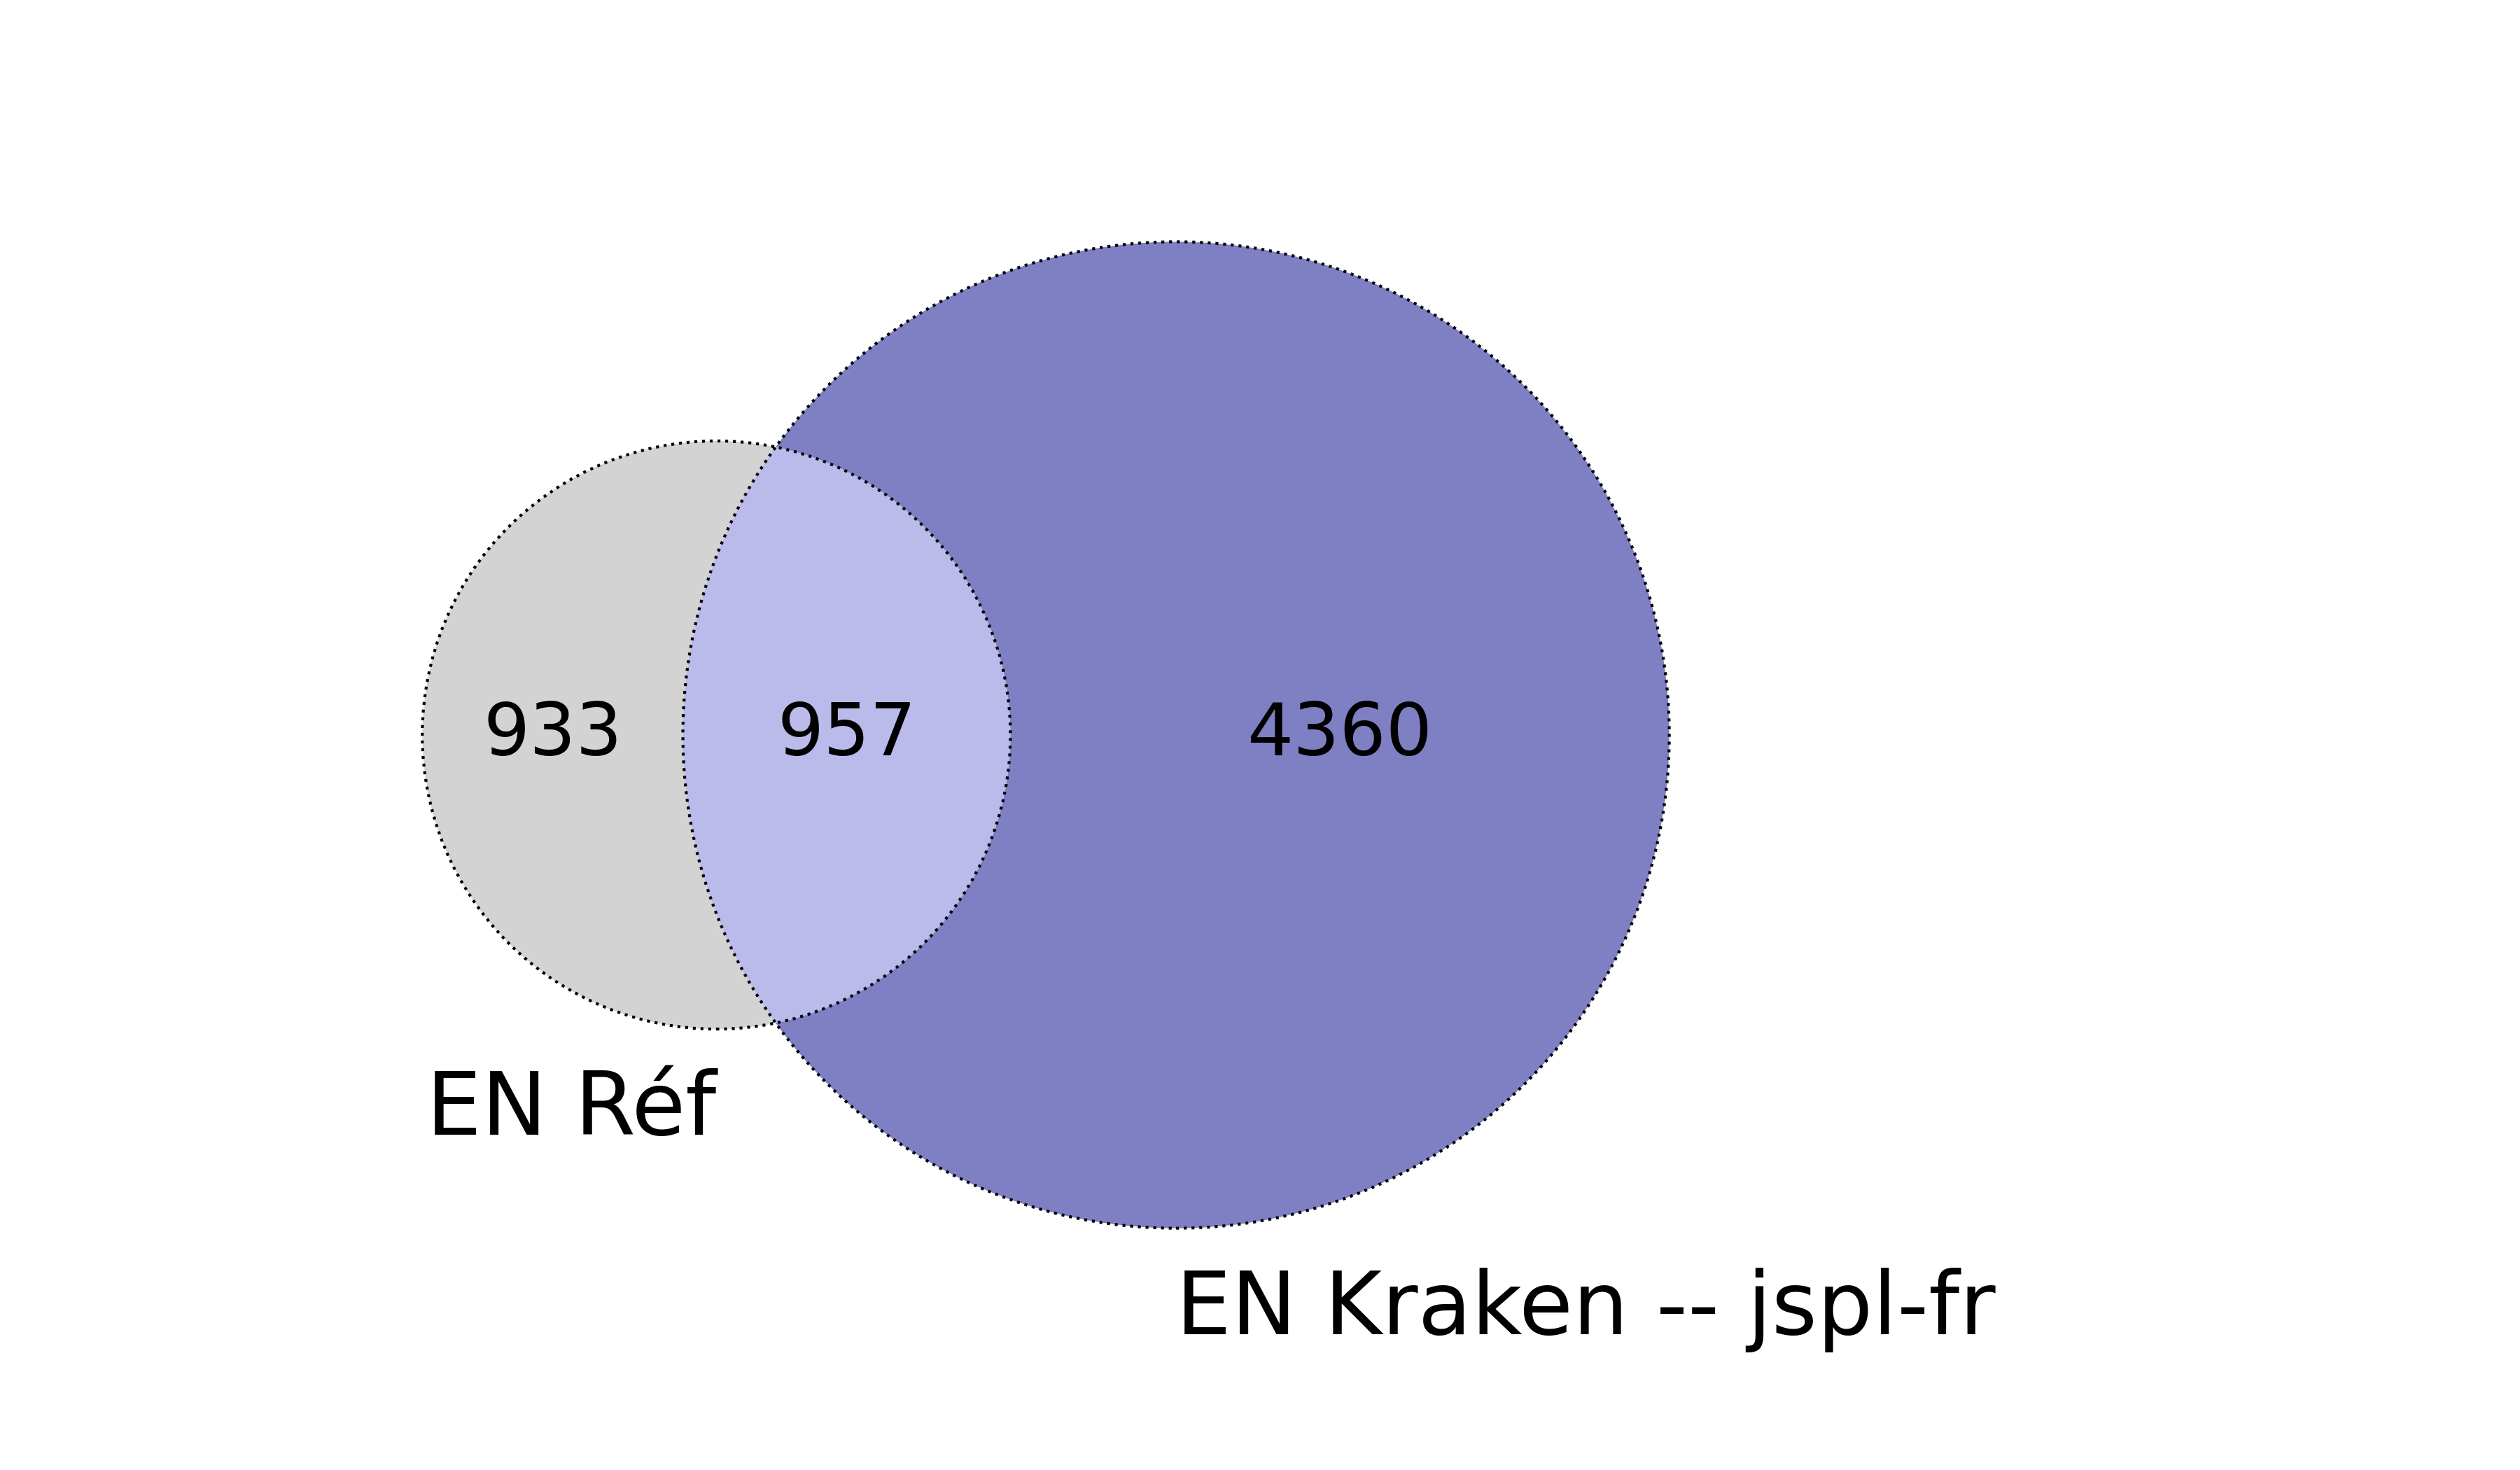
\includegraphics[width=1\textwidth]{IMAGES/INTERSECTIONS_GLOBALES/ELTeCFRA_Kraken -- jspl-fr_spacy-lg-concat_intersection.png} 
  \caption{Kraken corrigé Jspll pretrain --\texttt{spaCy\_lg}}
  \label{fig:ELTeCFRA_Kraken -- jspl-fr_spacy-lg-concat_intersection.png}
  \end{subfigure}
  \end{minipage}
  \begin{minipage}{7cm}
  \begin{subfigure}{1\textwidth}
  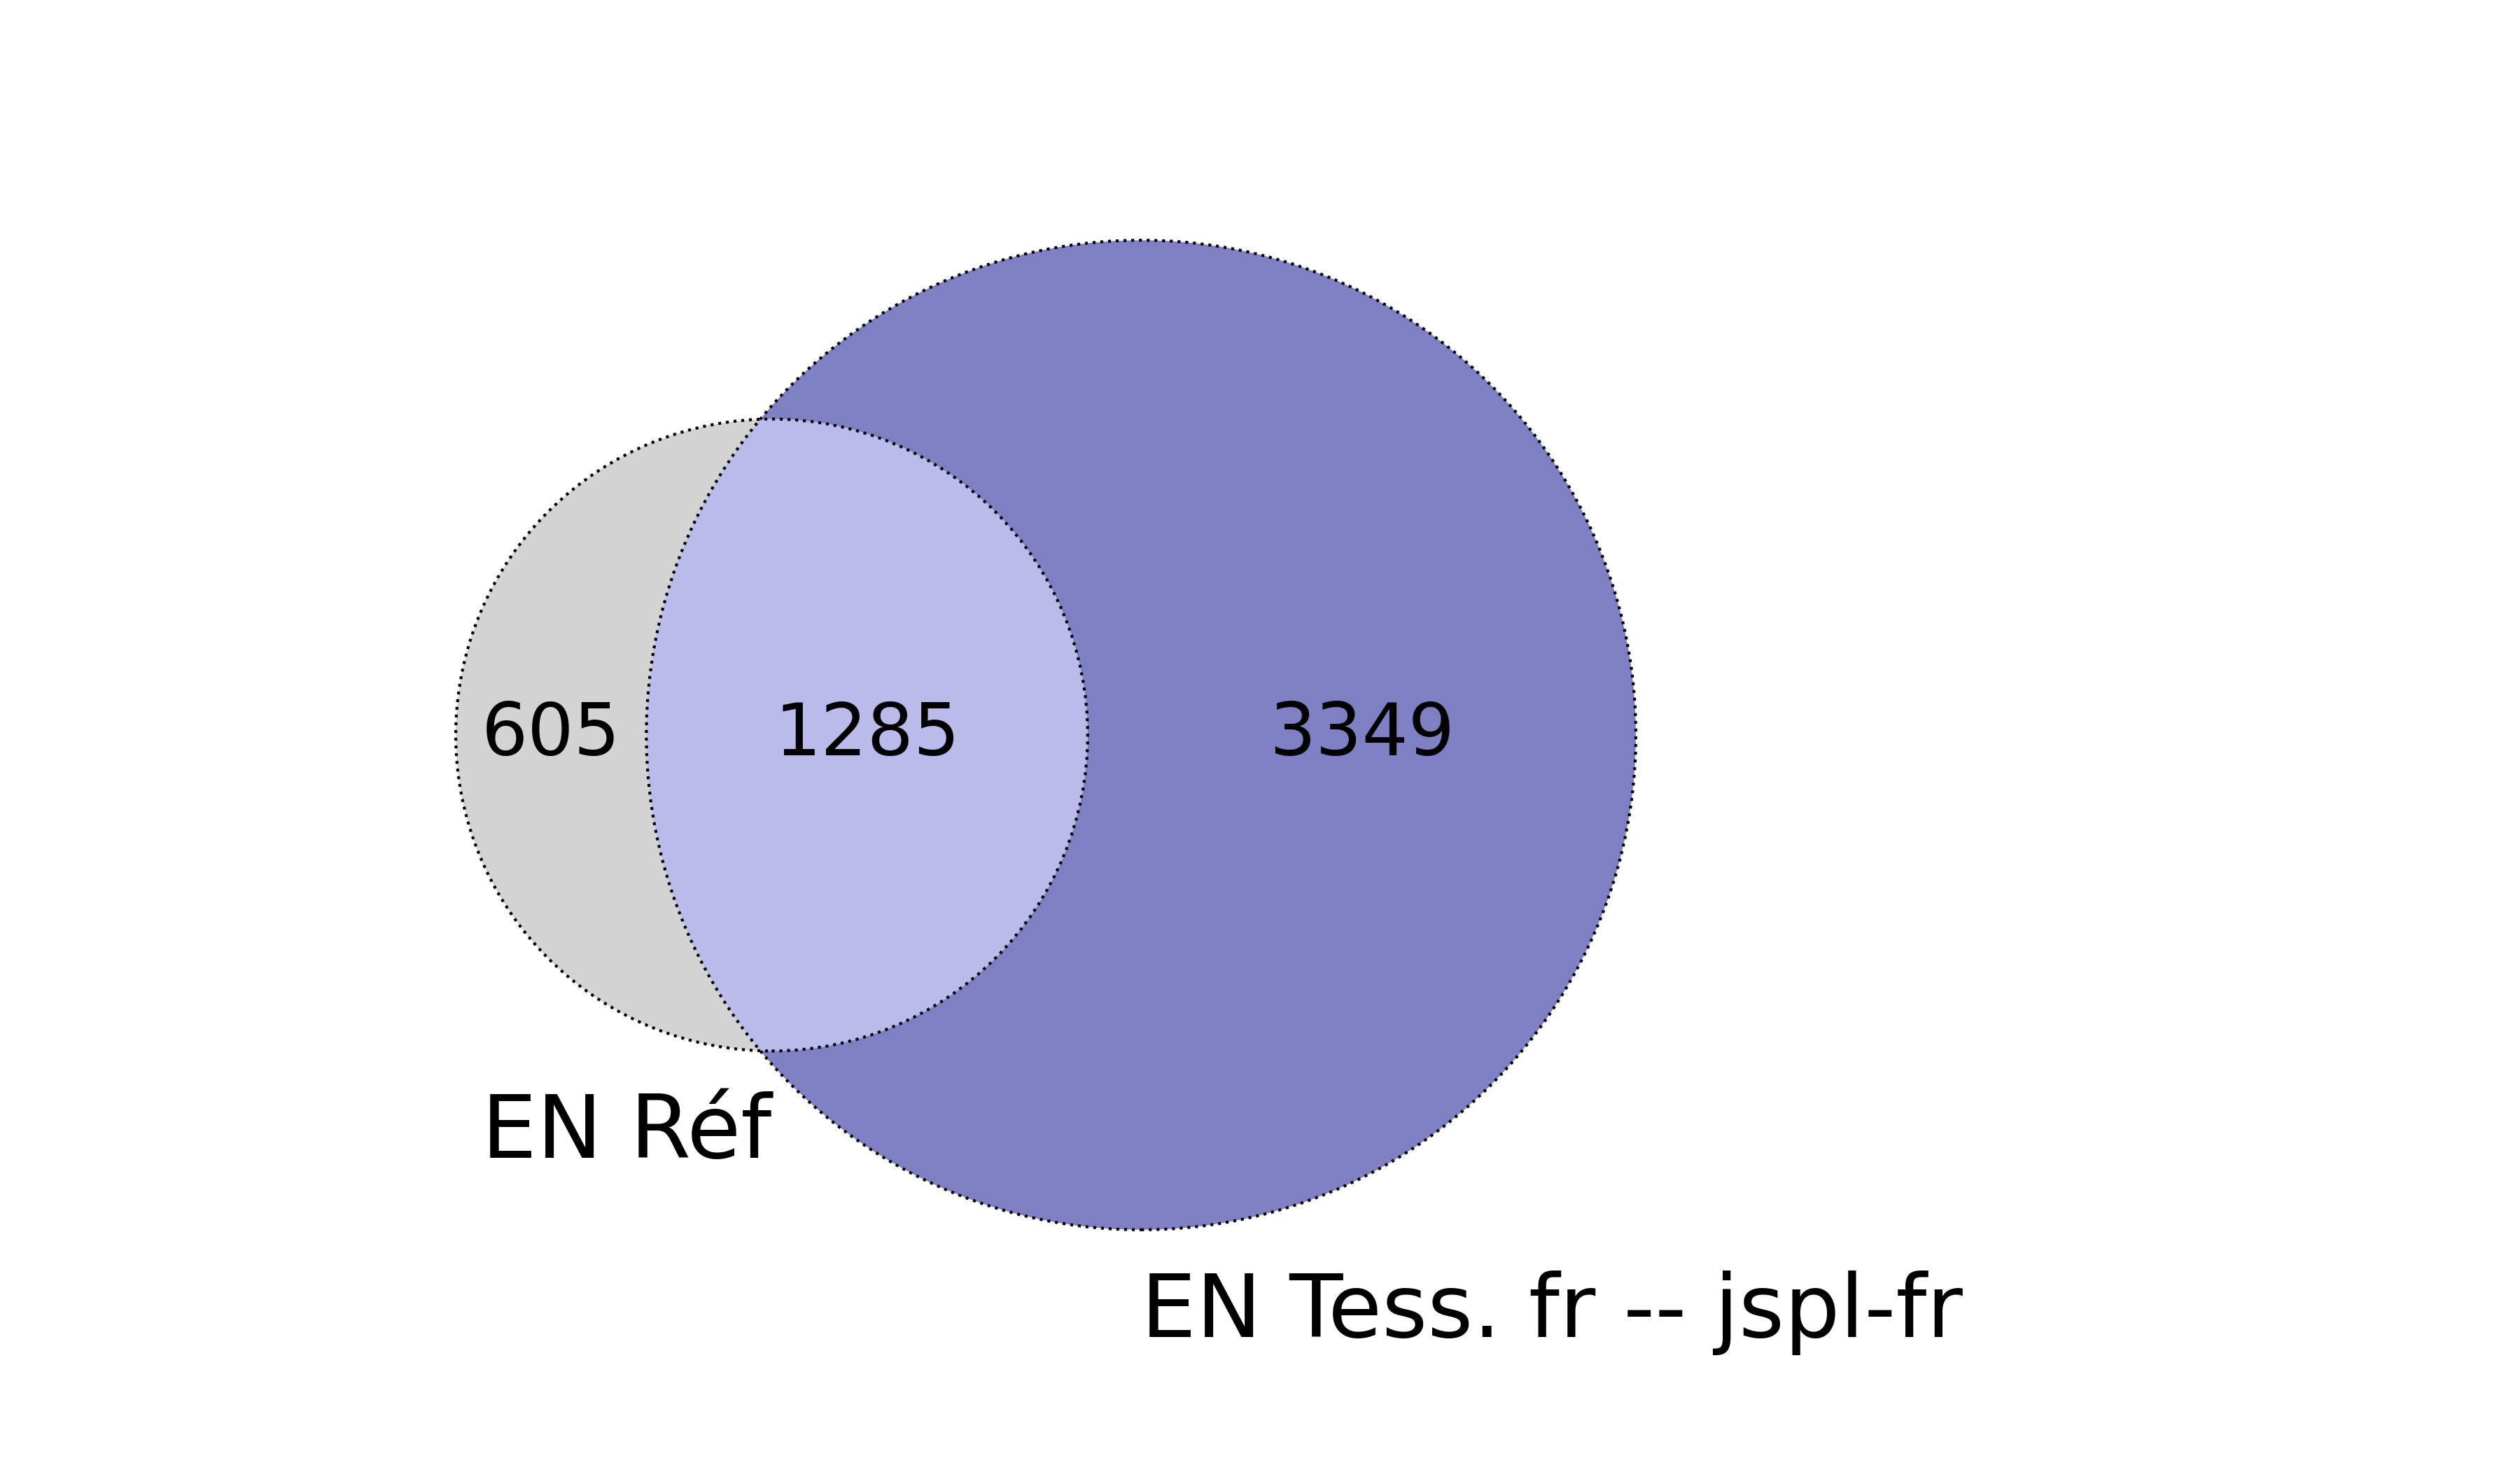
\includegraphics[width=1\textwidth]{IMAGES/INTERSECTIONS_GLOBALES/ELTeCFRA_Tess. fr -- jspl-fr_spacy-lg-concat_intersection.png} 
  \caption{Tess. fr. corrigé Jspll pretrain -- \texttt{spaCy\_lg}}
 \label{fig:ELTeCFRA_Tess. fr -- jspl-fr_spacy-lg-concat_intersection.png}
  \end{subfigure}
    \end{minipage}
\begin{minipage}{7cm}
  \begin{subfigure}{1\textwidth}
  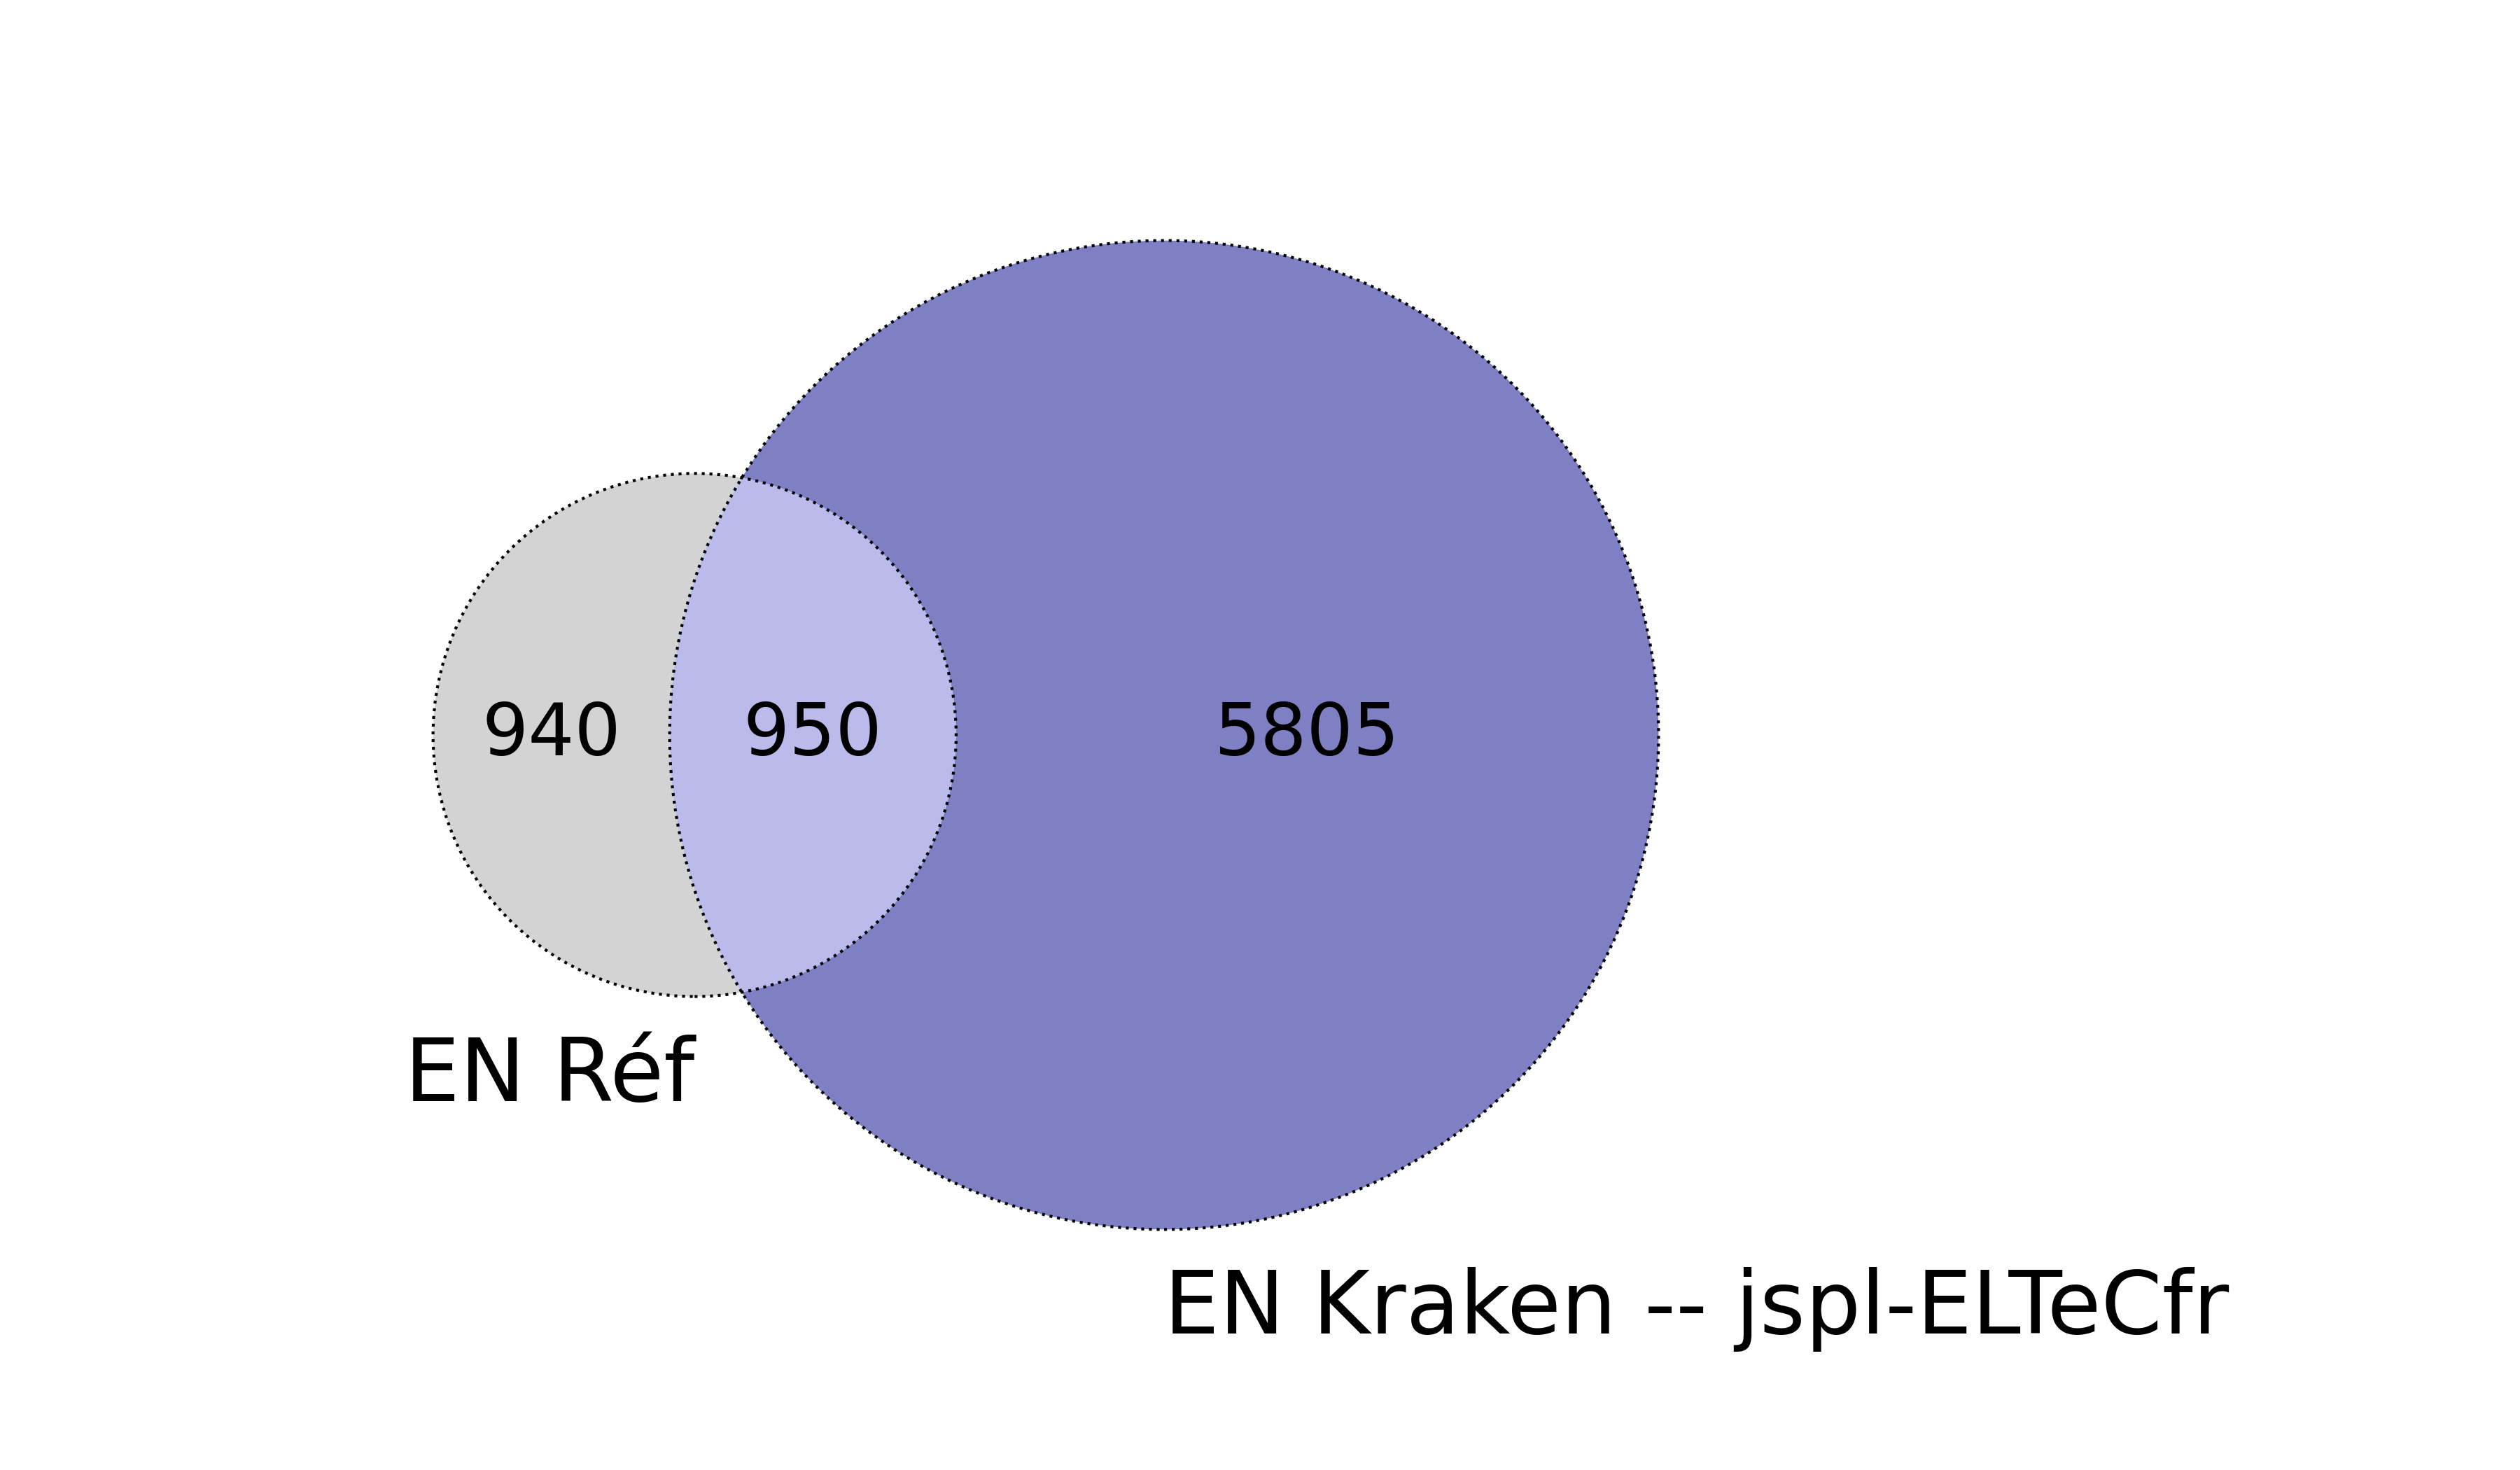
\includegraphics[width=1\textwidth]{IMAGES/INTERSECTIONS_GLOBALES/ELTeCFRA_Kraken -- jspl-ELTeCfr_spacy-lg-concat_intersection.png} 
  \caption{Kraken corrigé ELTeC-fr -- \texttt{spaCy\_lg}}
  \label{fig:ELTeCFRA_Kraken -- jspl-ELTeCfr_spacy-lg-concat_intersection}
  \end{subfigure}
  \end{minipage}
  \begin{minipage}{7cm}
  \begin{subfigure}{1\textwidth}
  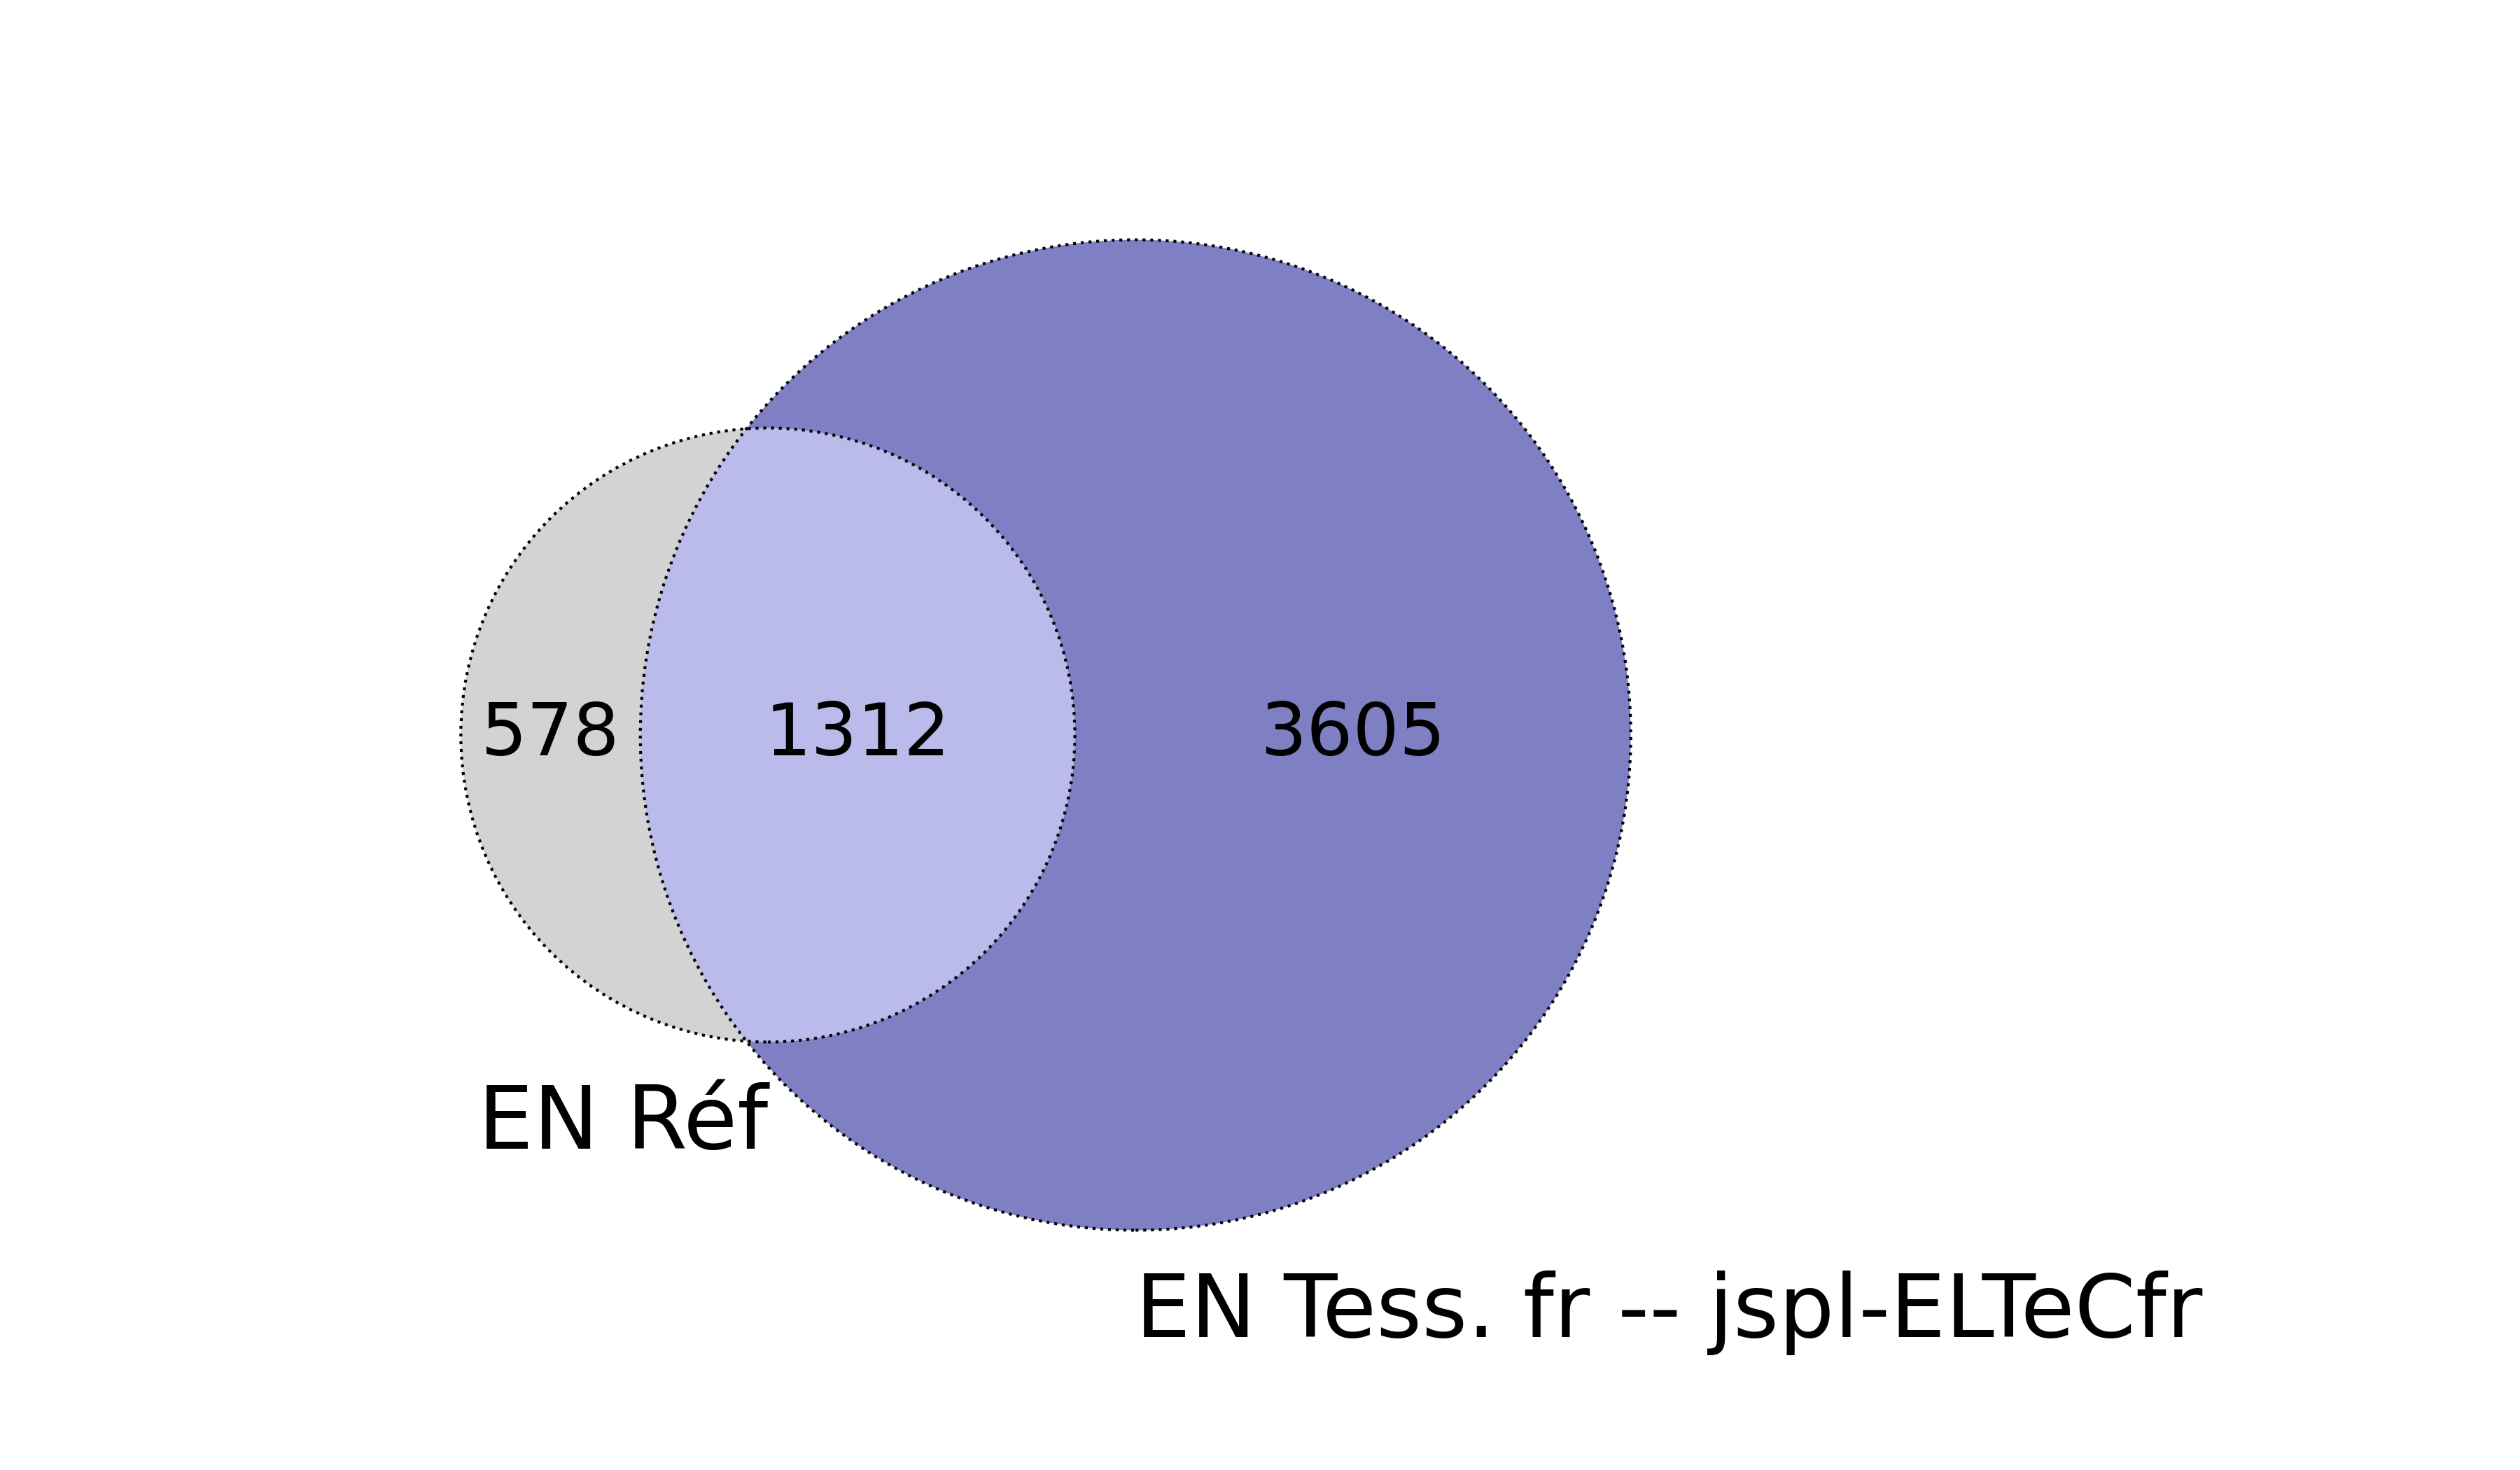
\includegraphics[width=1\textwidth]{IMAGES/INTERSECTIONS_GLOBALES/ELTeCFRA_Tess. fr -- jspl-ELTeCfr_spacy-lg-concat_intersection.png} % nouvelle figure ici avec Tess. fr. corrigé avec spaCy_lg
  \caption{Tess. fr. corrigé ELTeC-fr -- \texttt{spaCy\_lg}}
  \label{fig:ELTeCFRA_Tess -- jspl-ELTeCFR_spacy-lg-concat_intersection}
  \end{subfigure}
    \end{minipage}
%\caption{Intersections pour les configurations (\ref{fig:ELTeCFRA_Kraken -- jspl-fr_spacy-lg-concat_intersection.png
%}-\ref{fig:ELTeCFRA_Tess -- spacy-lg-concat_intersection}) Kraken-\texttt{spaCy\_lg} et Tess. fr.-\texttt{spaCy\_lg} non corrigées, et (\ref{fig:ELTeCFRA_Kraken -- jspl-ELTeCfr_spacy-lg-concat_intersection}-\ref{fig:ELTeCFRA_Tess -- jspl-ELTeCFR_spacy-lg-concat_intersection}) les configurations équivalentes corrigées avec JamSpell (modèle ELTeC), pour le sous-corpus ELTeC français.}
\caption{Intersections pour les configurations Kraken-\texttt{spaCy\_lg} et Tess. fr.-\texttt{spaCy\_lg} corrigées avec JamSpell pré-entraîné (\ref{fig:ELTeCFRA_Kraken -- jspl-fr_spacy-lg-concat_intersection.png}-\ref{fig:ELTeCFRA_Tess. fr -- jspl-fr_spacy-lg-concat_intersection.png}), et les configurations équivalentes corrigées avec JamSpell (modèle ELTeC), pour le sous-corpus ELTeC français (\ref{fig:ELTeCFRA_Kraken -- jspl-ELTeCfr_spacy-lg-concat_intersection}-\ref{fig:ELTeCFRA_Tess -- jspl-ELTeCFR_spacy-lg-concat_intersection}).}
\label{fig:intersection_globale-kraken}
\end{figure}

Ce fait peut être lu à l'aune des observations présentées dans le tableau \ref{tab:typologie_erreurs-corr_ELTeCEng} rapportant la typologie des erreurs de corrections. Autrement dit, la correction automatique ne transforme pas toutes les EN contaminées par la ROC en EN corrigées strictement associables avec les EN du groupe de référence. Ainsi les BOIC (``Morlincourt'' qui devient ``Martincourt''), se cumulant aux EN contaminées MOI (``Morlincourtl'' qui reste ``Morlincourtl''), rendent les résultats des intersections moins bons. Il semble qu'en moyenne pour les corpus ELTeC français, anglais et portugais et celui de la TGB la correction automatique avec le modèle entraîné sur une partie de chaque sous-corpus ELTeC fasse perdre 5\% des EN dans l'intersection avec Kraken et 10\% avec Tesseract, alors que concernant les modèles pré-entraînés on perd 3\% avec Kraken et 9\% avec Tesseract. Cette expérience est l'occasion de démontrer les limites d'une évaluation stricte de la REN sur des textes bruités et leurs versions corrigées. Il est notable que les contaminations de ROC d'une part et de la correction automatique d'autre part ne sont pas véritablement un frein à la REN, mais l'évaluation automatique des résultats n'est pas triviale.

%%%%%%%%%%%%%%%% Ancienne figure avec les intersections pour la config Tess-spaCy_lg corrigées avec le modèle pré-entraîné de JamSpell et le modèle ELTeC, pour le sous-corpus ELTeC fr %%%%%%%%%%%%%%%%%%

%\begin{figure}[h!]
%%    \begin{minipage}{7cm}
%%  \begin{subfigure}{1\textwidth}
%%  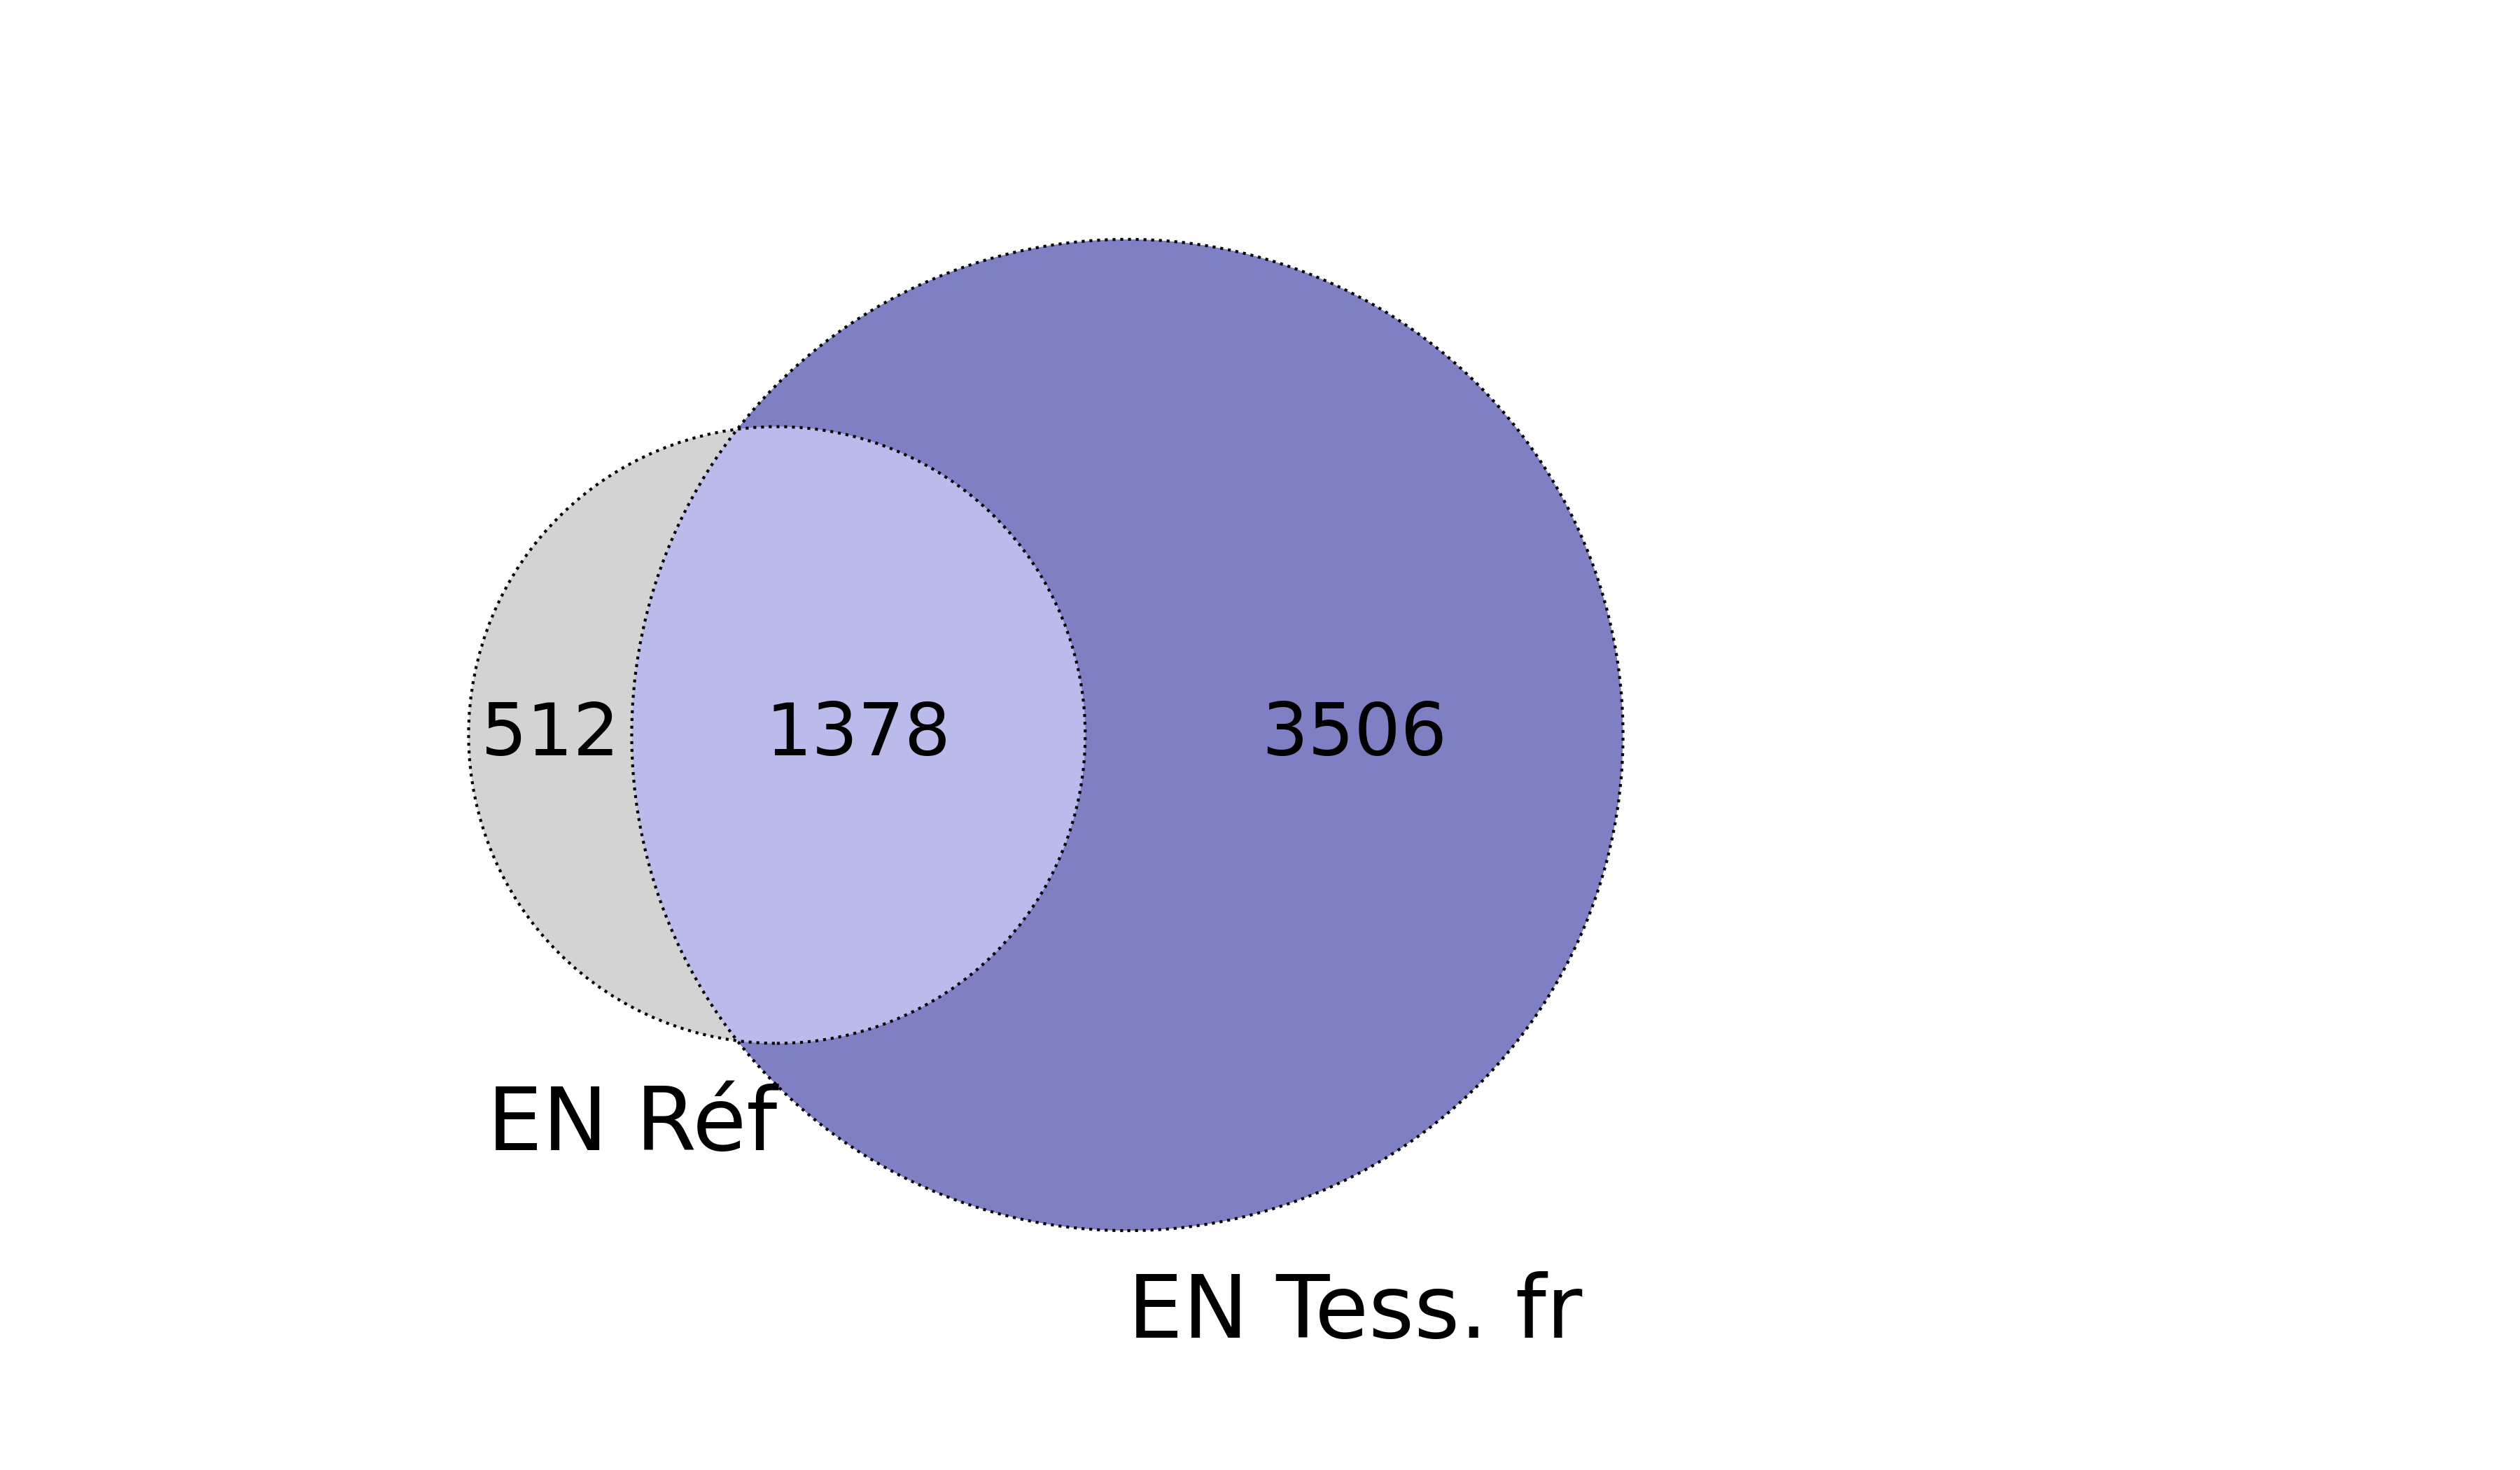
\includegraphics[width=1\textwidth]{IMAGES/INTERSECTIONS_GLOBALES/ELTeCFRA_Tess. fr_spacy-lg-concat_intersection.png} 
%%  \caption{Tess. fr. --\texttt{spaCy\_lg}}
%%  \label{fig:ELTeCFRA_Tess. fr_spacy-lg-concat_intersection}
%%  \end{subfigure}
%%  \end{minipage}
%%  \begin{minipage}{7cm}
%%  \begin{subfigure}{1\textwidth}
%%  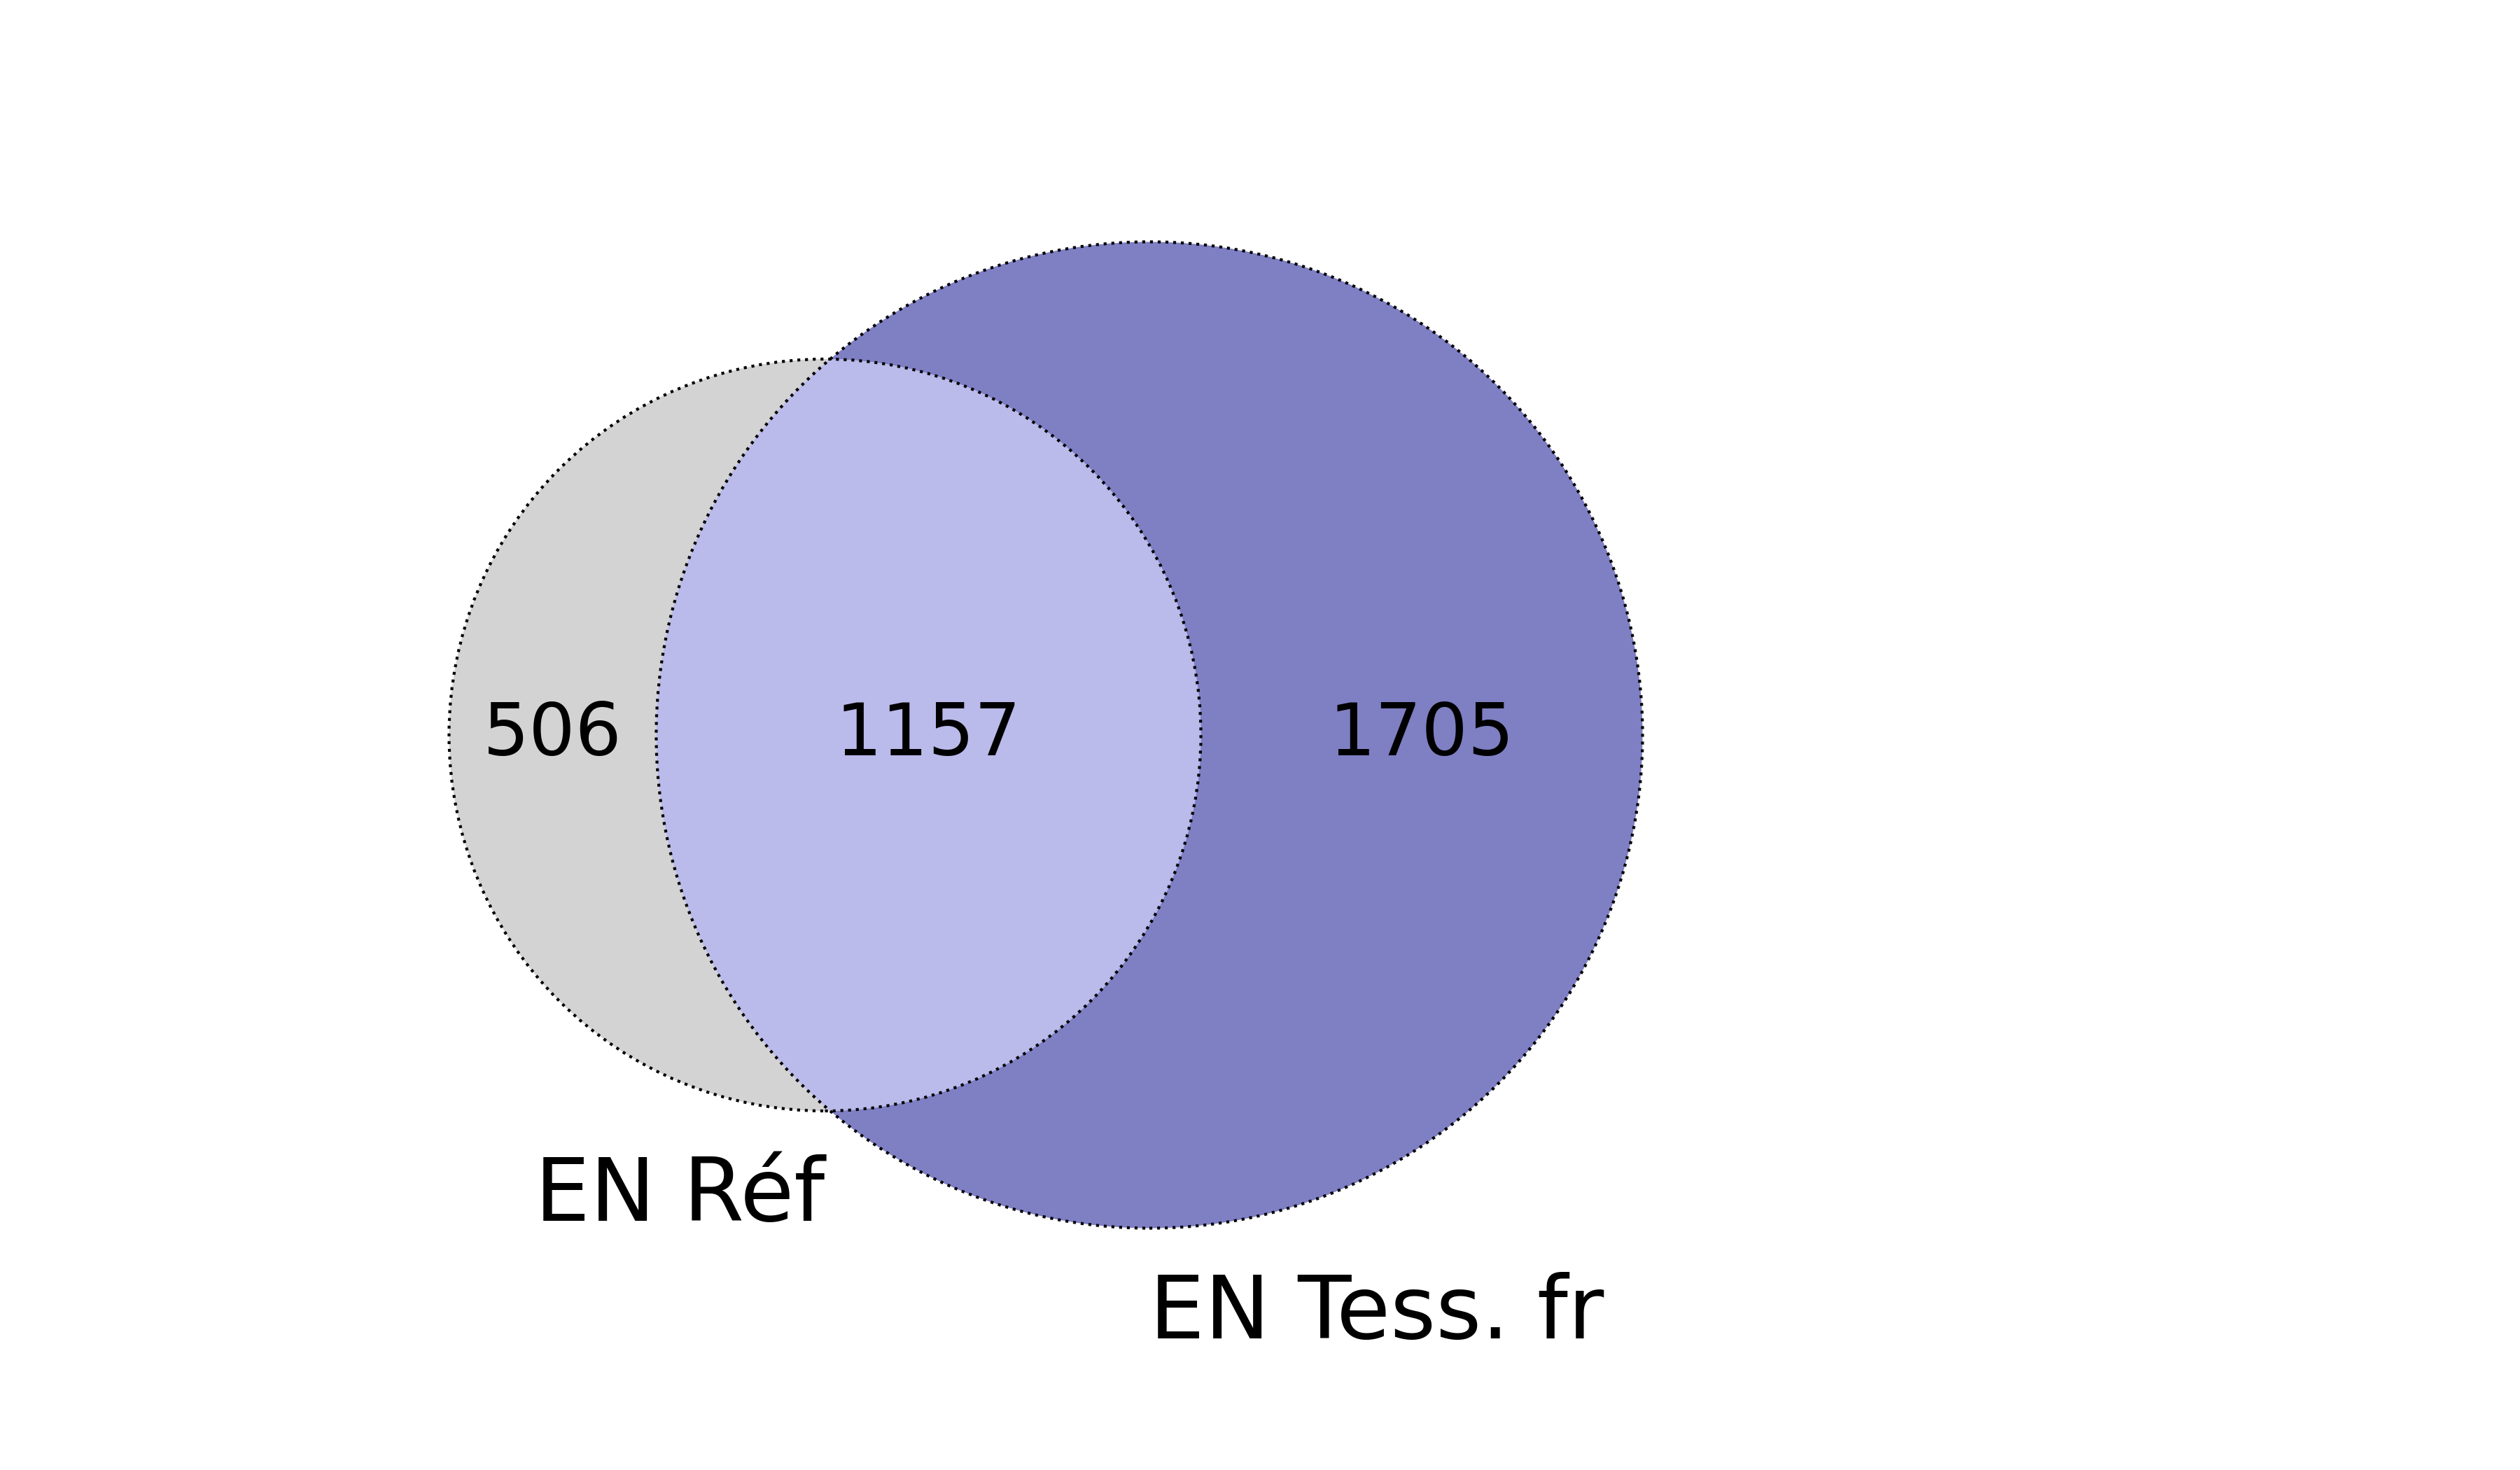
\includegraphics[width=1\textwidth]{IMAGES/INTERSECTIONS_GLOBALES/ELTeCFRA_Tess. fr_stanza-concat_intersection.png}
%%  \caption{Tess. fr. -- \texttt{stanza}}
%% % \label{fig:ELTeCFRA_Tess. fr_stanza-concat_intersection}
%%  \end{subfigure}
%%    \end{minipage}
%%\begin{minipage}{7cm}
%%  \begin{subfigure}{1\textwidth}
%%  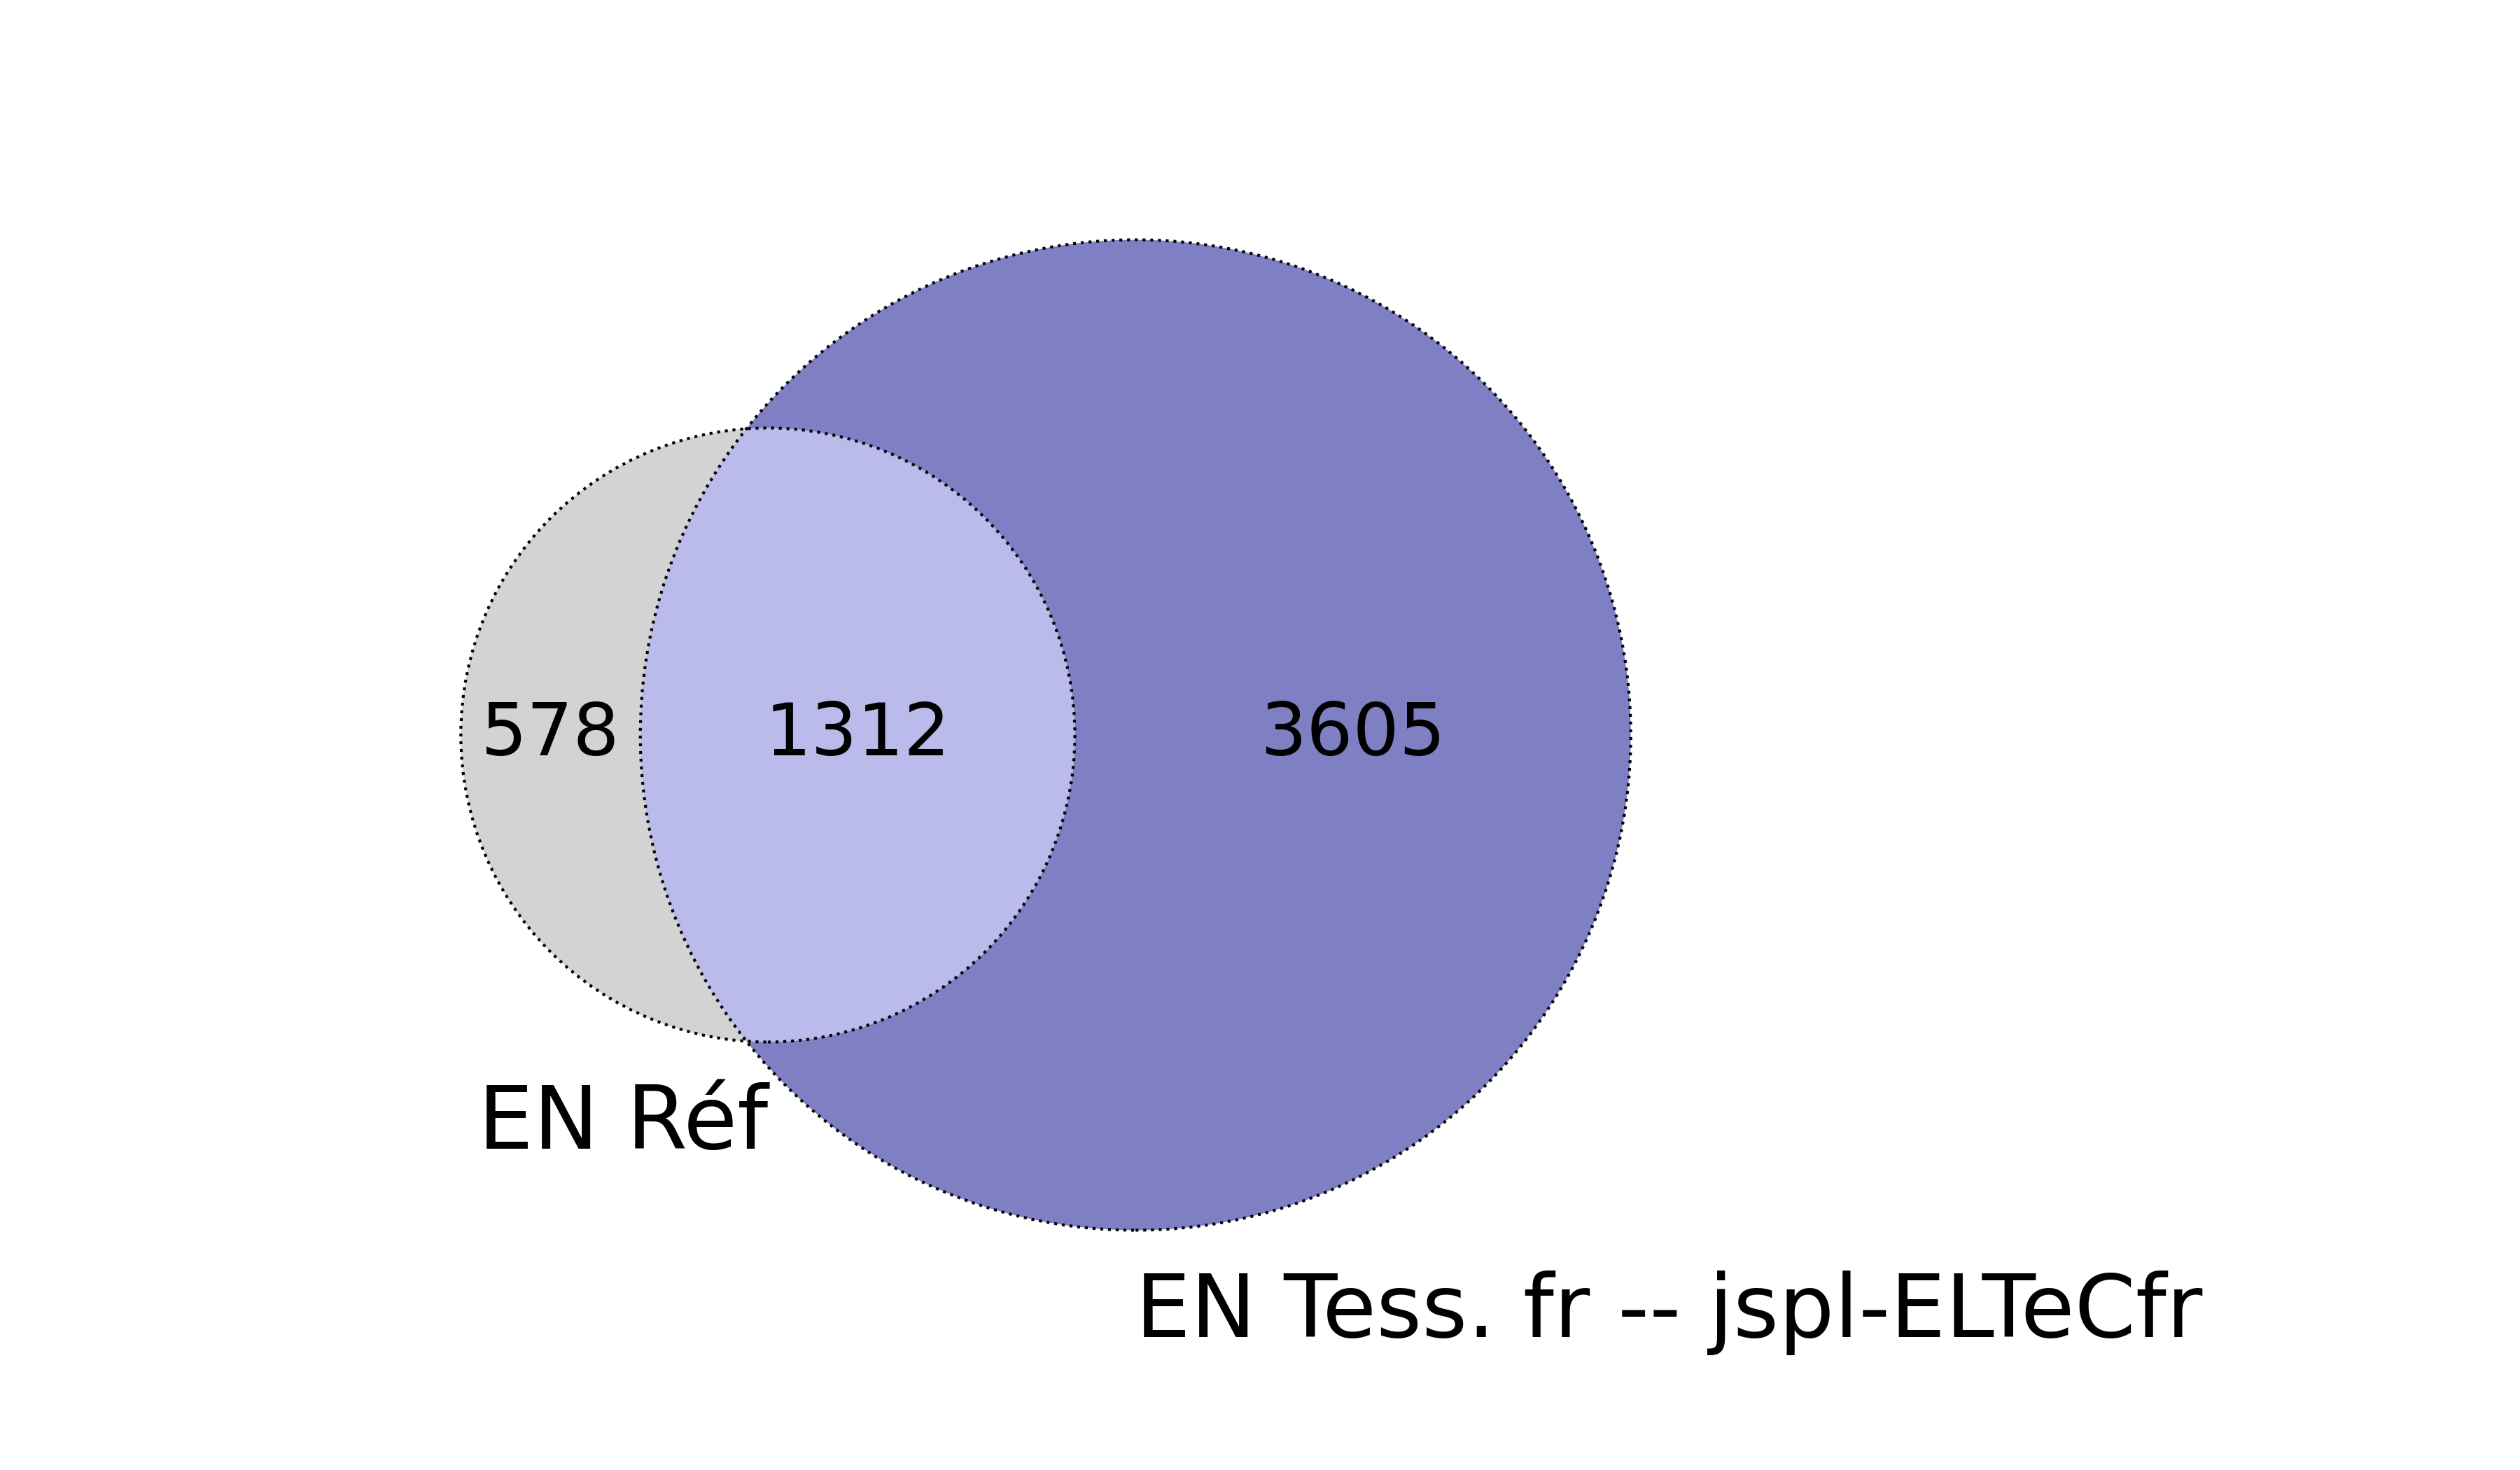
\includegraphics[width=1\textwidth]{IMAGES/INTERSECTIONS_GLOBALES/ELTeCFRA_Tess. fr -- jspl-ELTeCfr_spacy-lg-concat_intersection.png} 
%%  \caption{Tess. fr. corrigé -- \texttt{spaCy\_lg}}
%%  \label{fig:ELTeCFRA_Tess. fr -- jspl-ELTeCfr_spacy-lg-concat_intersection}
%%  \end{subfigure}
%%  \end{minipage}
%  \begin{minipage}{7cm}
%  \begin{subfigure}{1\textwidth}
%  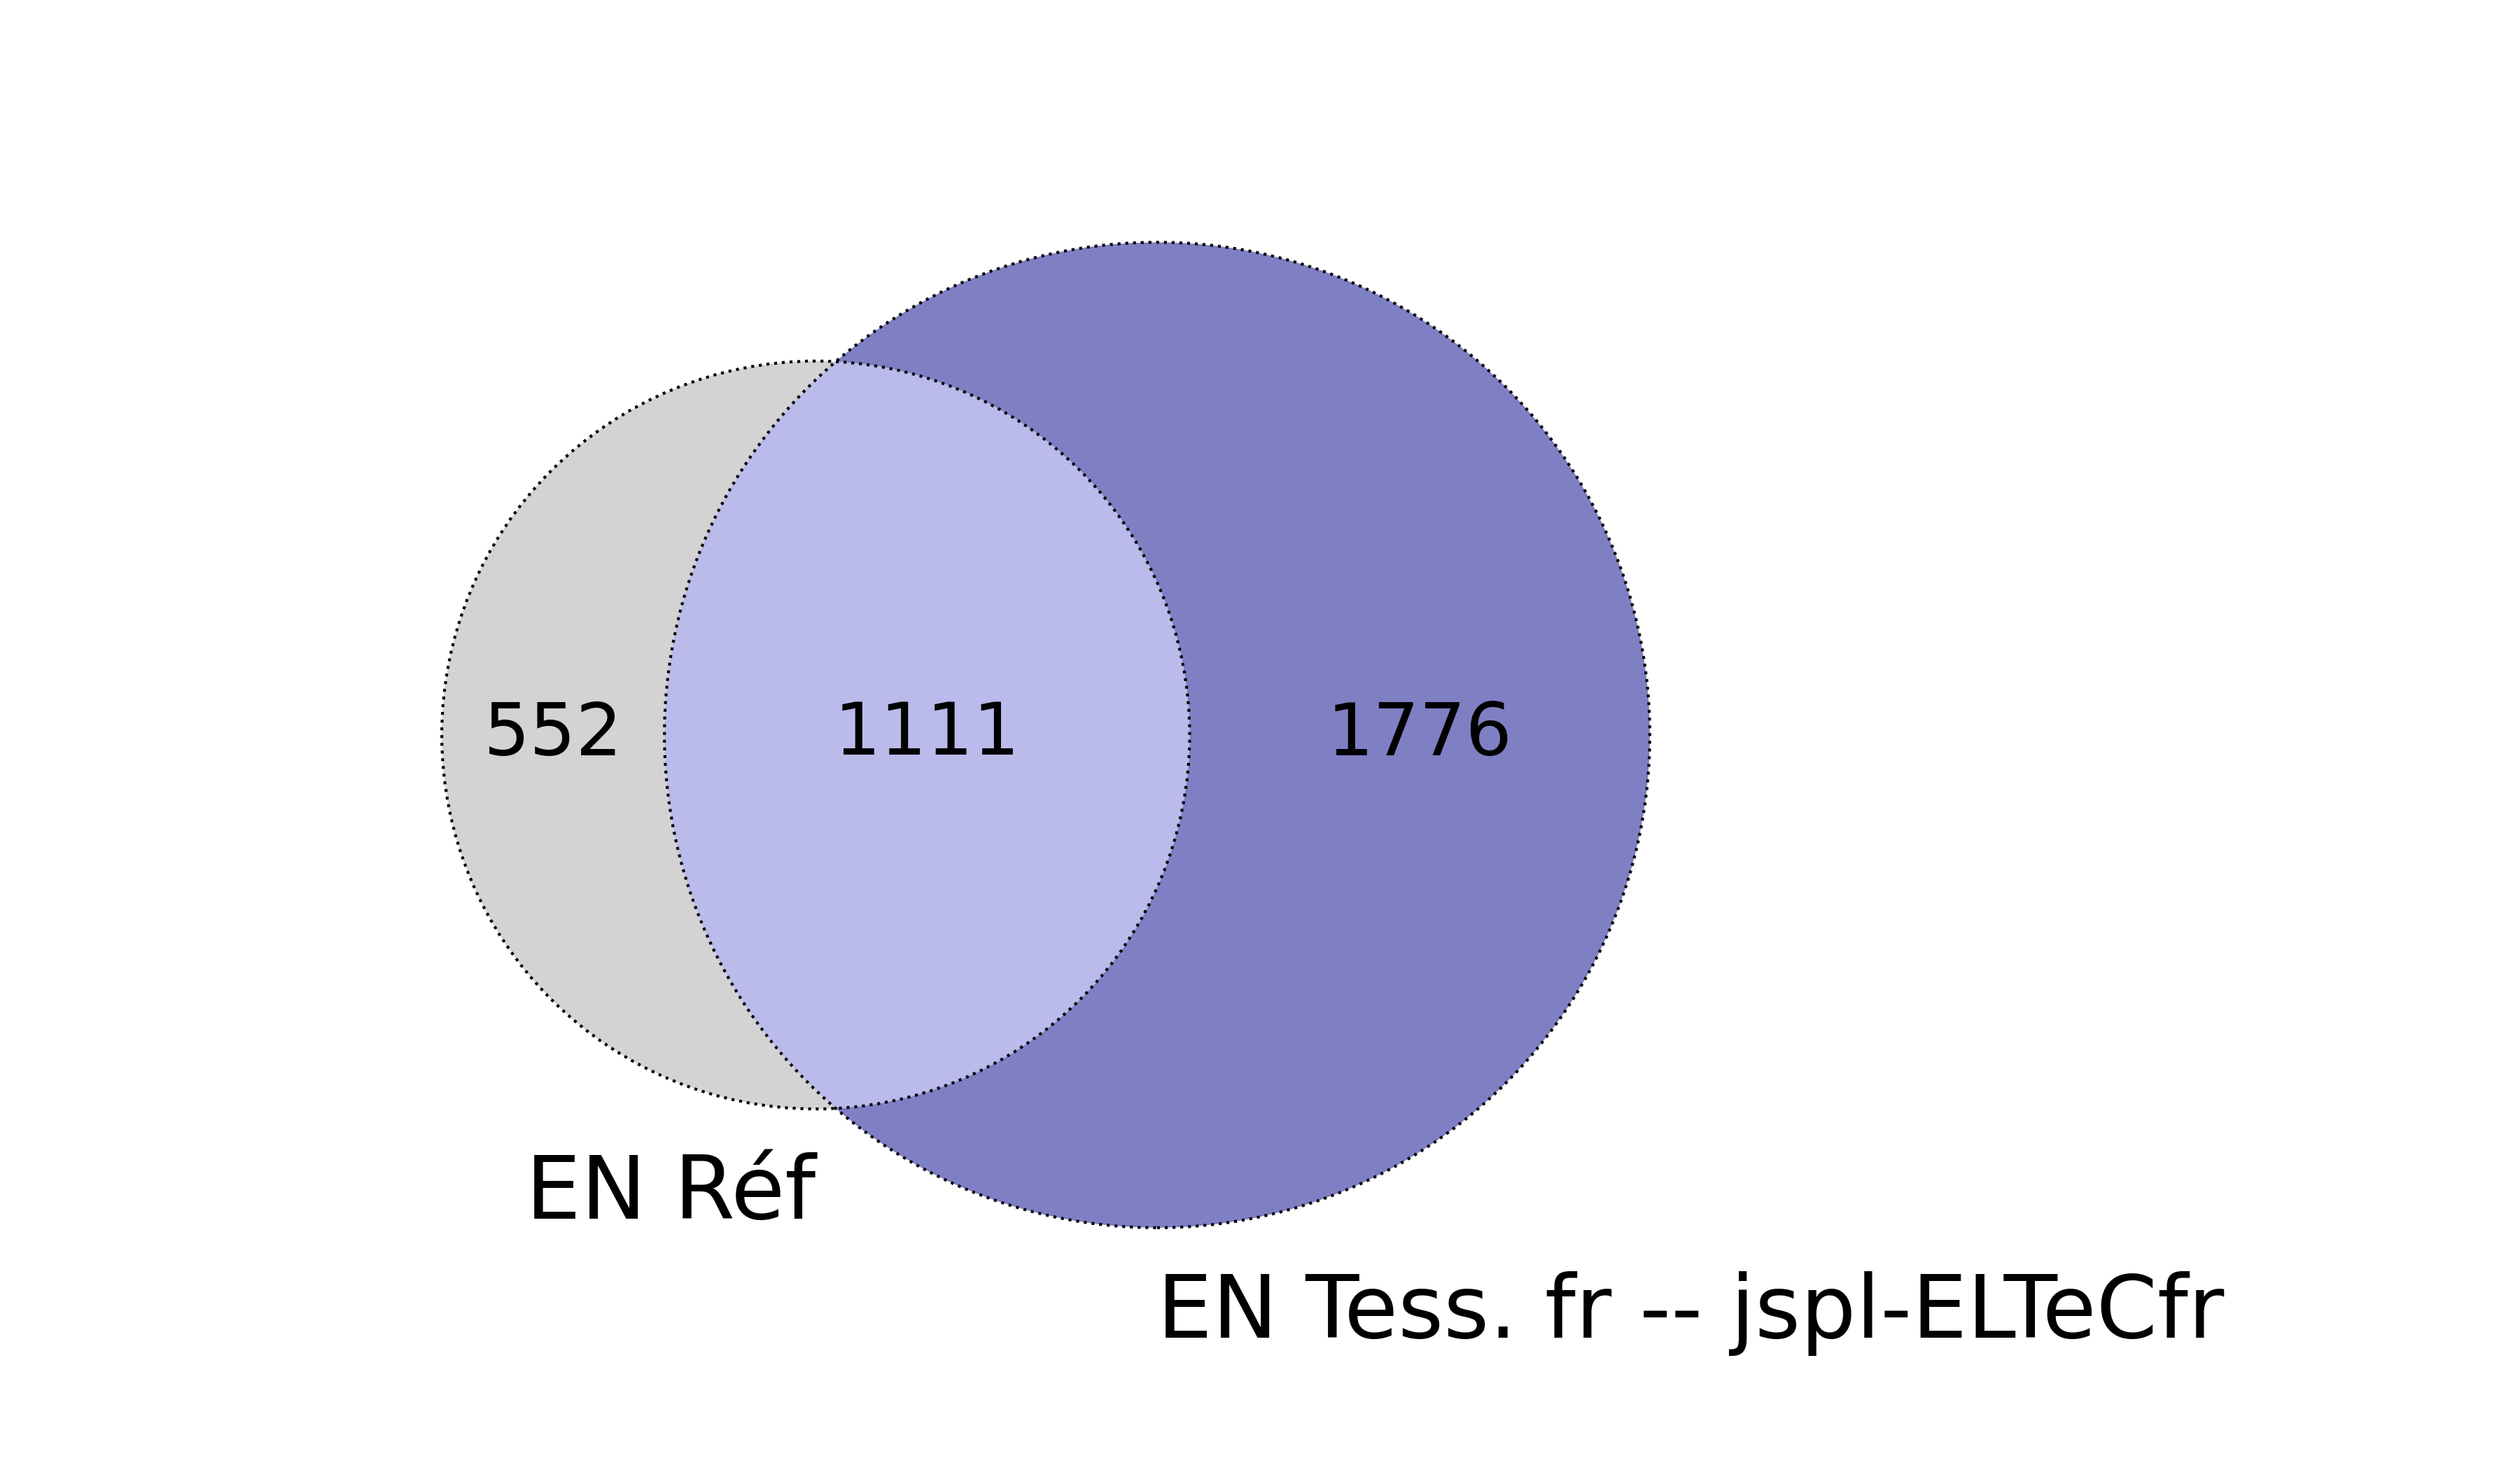
\includegraphics[width=1\textwidth]{IMAGES/INTERSECTIONS_GLOBALES/ELTeCFRA_Tess. fr -- jspl-ELTeCfr_stanza-concat_intersection.png}
%  \caption{Tess. fr. corrigé -- \texttt{stanza}}
%  \label{fig:ELTeCFRA_Tess. fr -- jspl-ELTeCfr_stanza-concat_intersection}
%  \end{subfigure}
%    \end{minipage}
%\begin{minipage}{7cm}
%  \begin{subfigure}{1\textwidth}
%  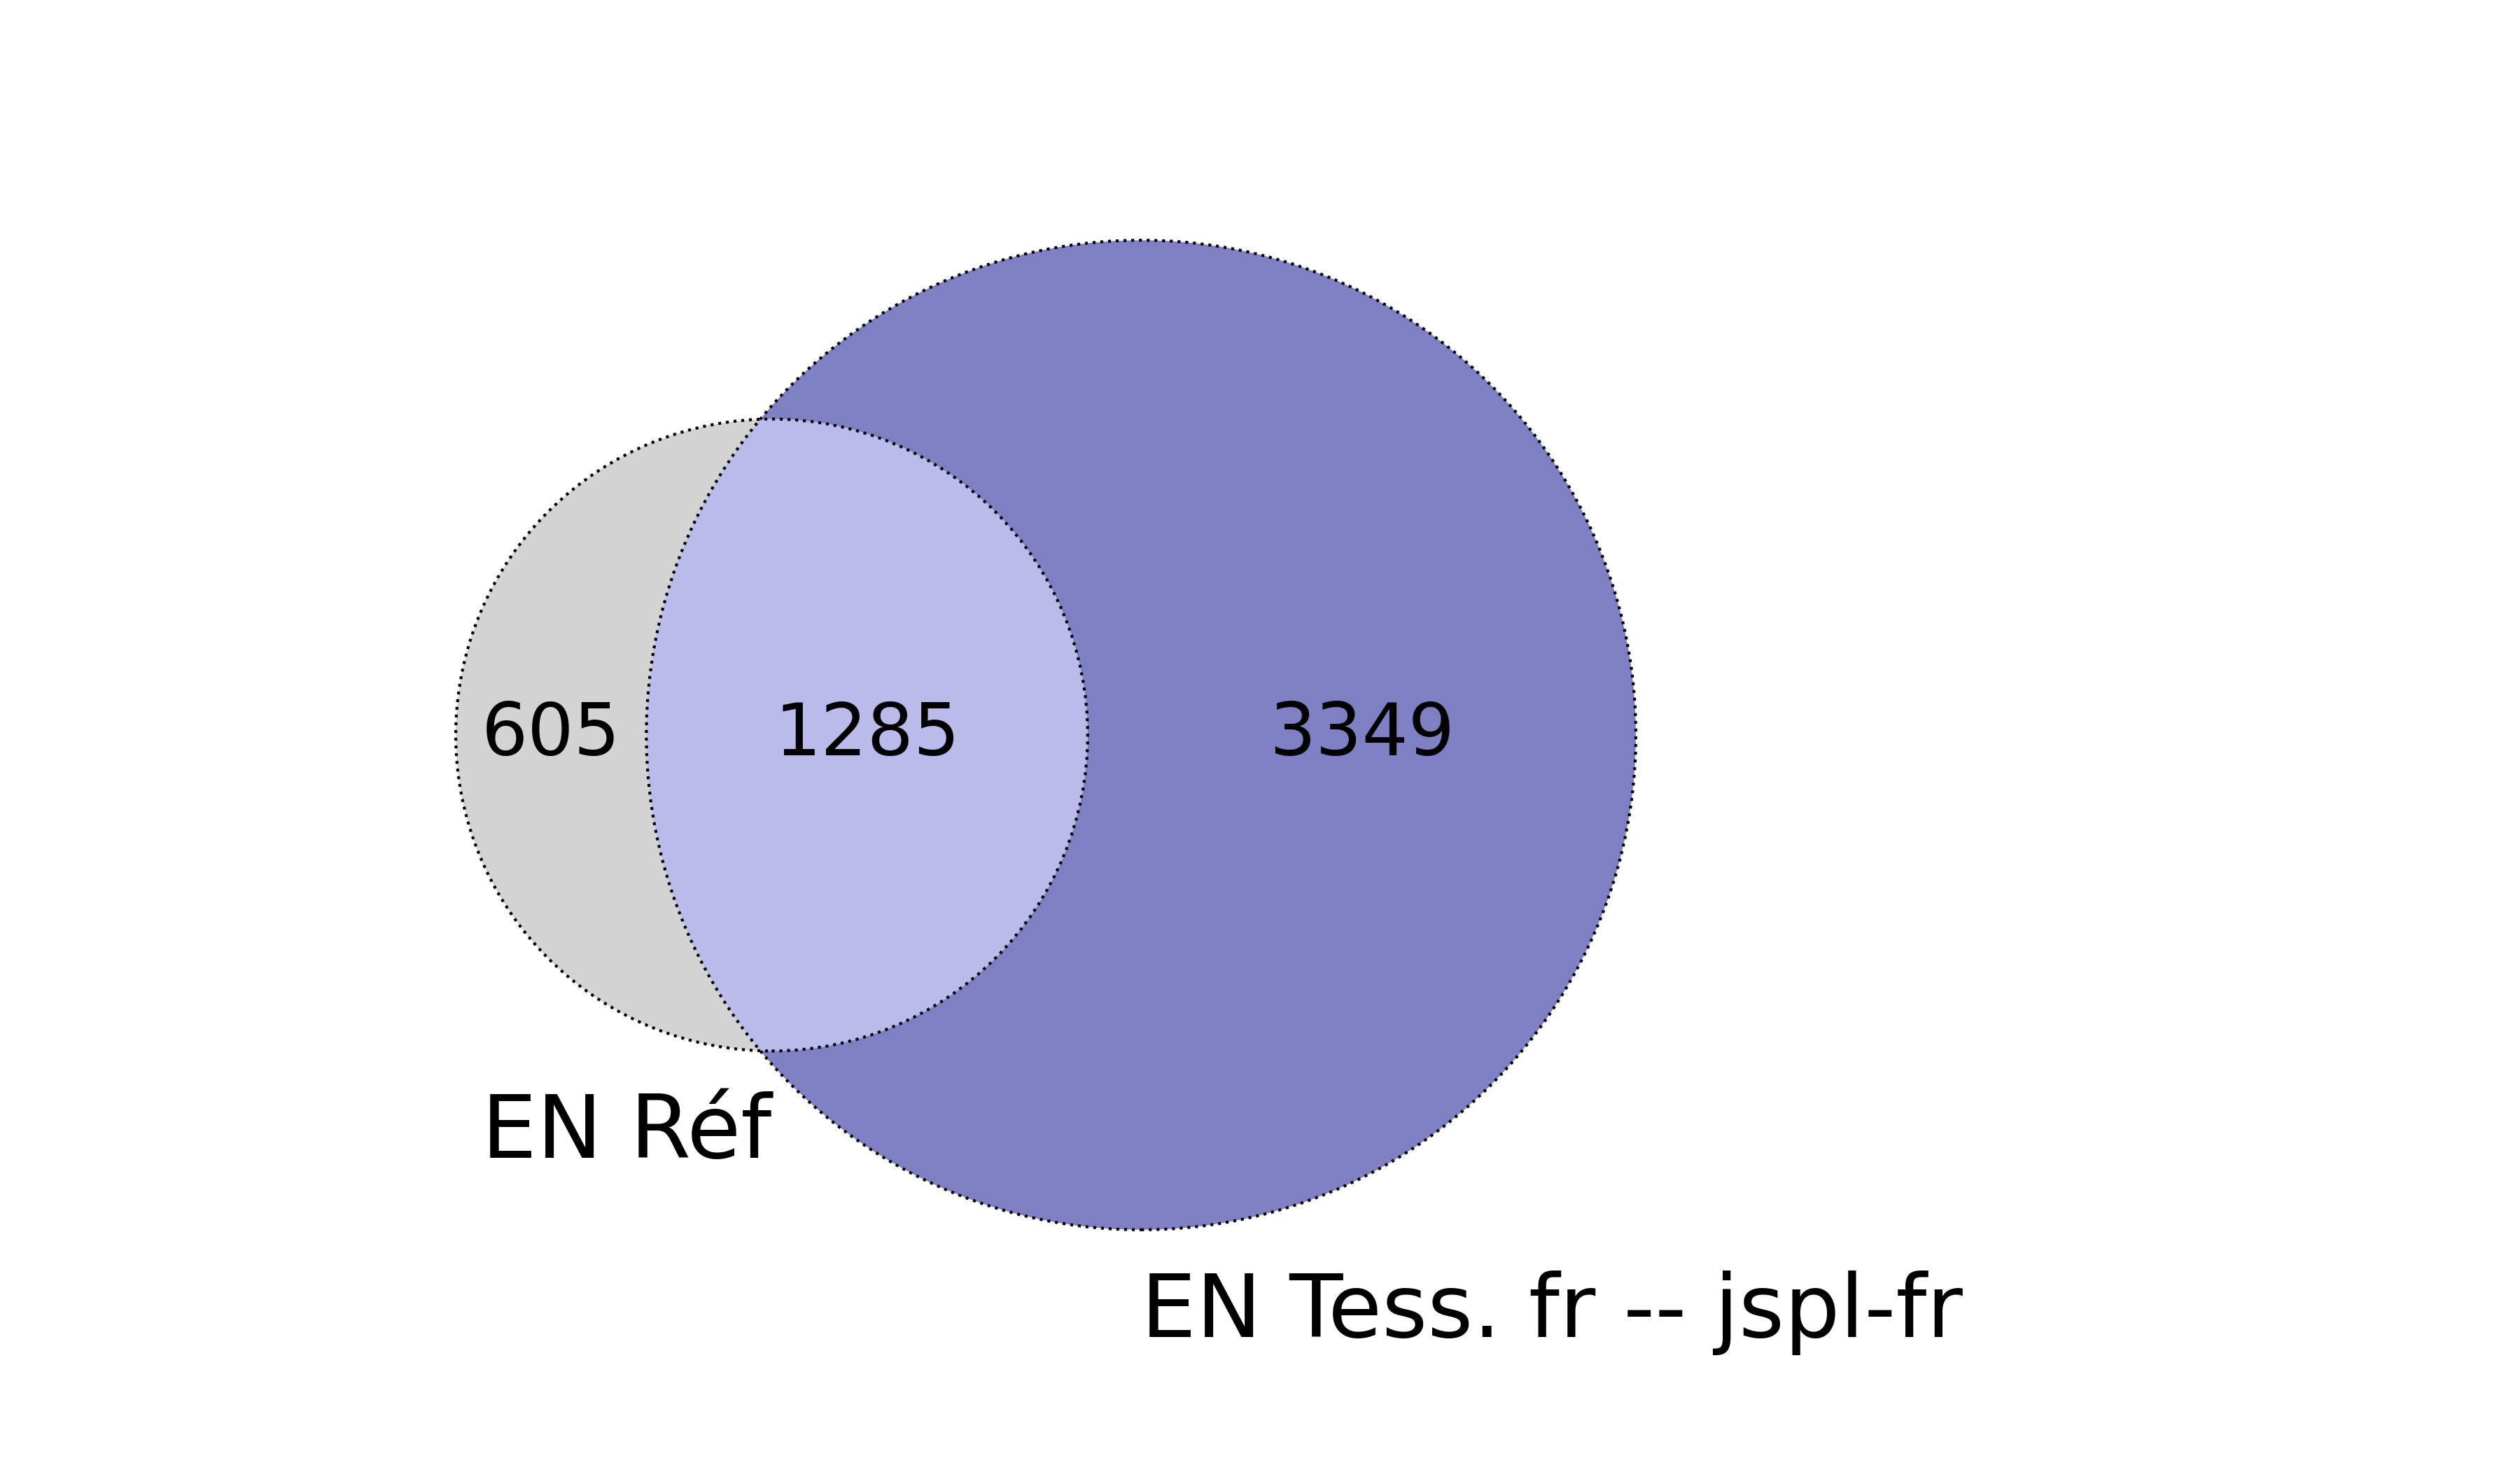
\includegraphics[width=1\textwidth]{IMAGES/INTERSECTIONS_GLOBALES/ELTeCFRA_Tess. fr -- jspl-fr_spacy-lg-concat_intersection.png} 
%  \caption{Tess. fr. corrigé -- \texttt{spaCy\_lg}}
%  \label{fig:ELTeCFRA_Tess. fr -- jspl-fr_spacy-lg-concat_intersection}
%  \end{subfigure}
%  \end{minipage}
%  \begin{minipage}{7cm}
%  \begin{subfigure}{1\textwidth}
%  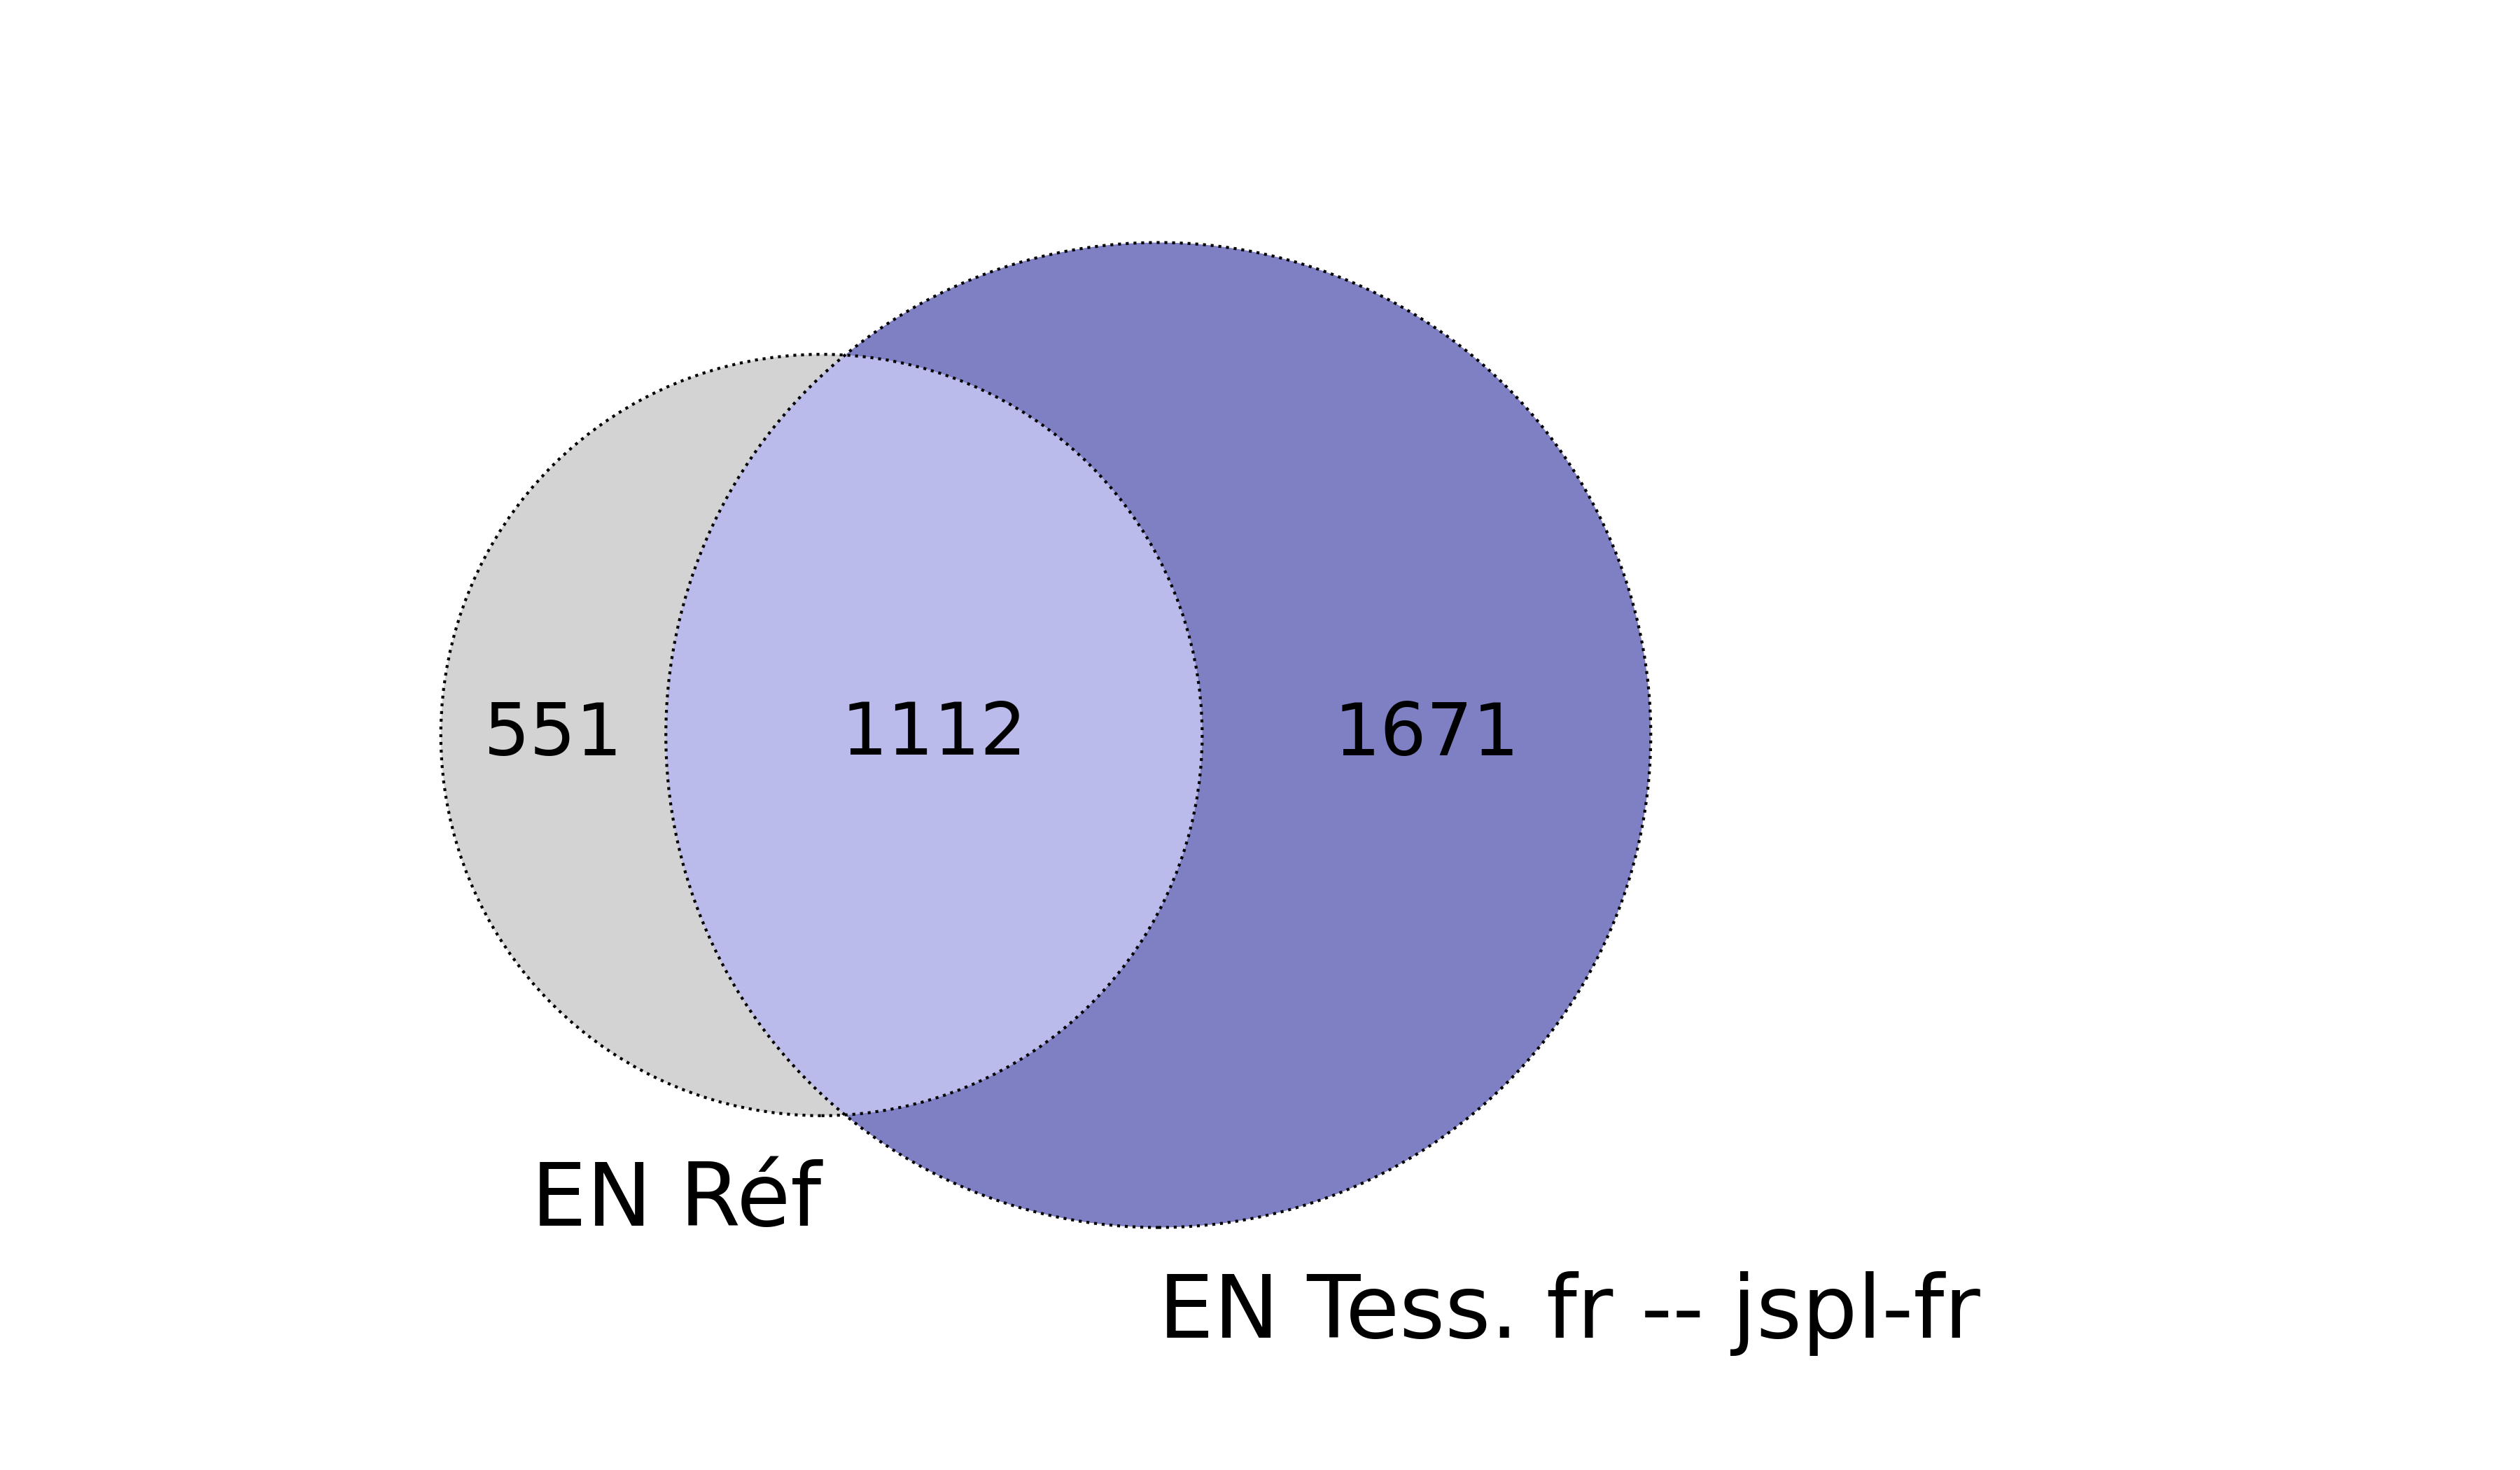
\includegraphics[width=1\textwidth]{IMAGES/INTERSECTIONS_GLOBALES/ELTeCFRA_Tess. fr -- jspl-fr_stanza-concat_intersection.png}
%  \caption{Tess. fr. corrigé -- \texttt{stanza}}
%  \label{fig:ELTeCFRA_Tess. fr -- jspl-fr_stanza-concat_intersection}
%  \end{subfigure}
%    \end{minipage}
%\caption{Intersections pour la configuration Tess-\texttt{spaCy\_lg} corrigées avec le modèle pré-entrainer de JamSpell et le modèle ELTeC, pour le sous-corpus ELTeC français.}
%\label{fig:intersection-globale-tess}
%\end{figure}
\subsection{Comment dépasser les problèmes d'alignements ? }
\label{subsec:ditances_creux_COR-OCR-IMPACT-NER}
\subsubsection{Mesures de distance textuelle}

Dans le but d'approfondir nos évaluation et de dépasser les verrous de l'évaluation stricte, nous employons des mesures de distance textuelle afin de rendre plus souple nos critères d'évaluation des résultats de REN sur les sorties de ROC bruitées et leurs corrections automatiques. Nous avons privilégié les métriques de Jaccard et cosinus car elles sont considérées comme des mesures de référence quand il est question de (dis)similarité textuelle \cite{buscaldi2020calcul}. Les sous-figures \ref{fig:ELTeC-Por_REF_jaccard}-\ref{fig:ELTeC-Por_REF_cosinus} illustrent les résultats obtenus pour les textes de référence et les différentes versions de ROC pour le corpus ELTeC portugais avec les mesures de jaccard et cosinus, et les résultats pour les autres corpus de notre études sont similaires.

\begin{figure}[h!]
   \centering
      \begin{subfigure}{0.45\textwidth}
  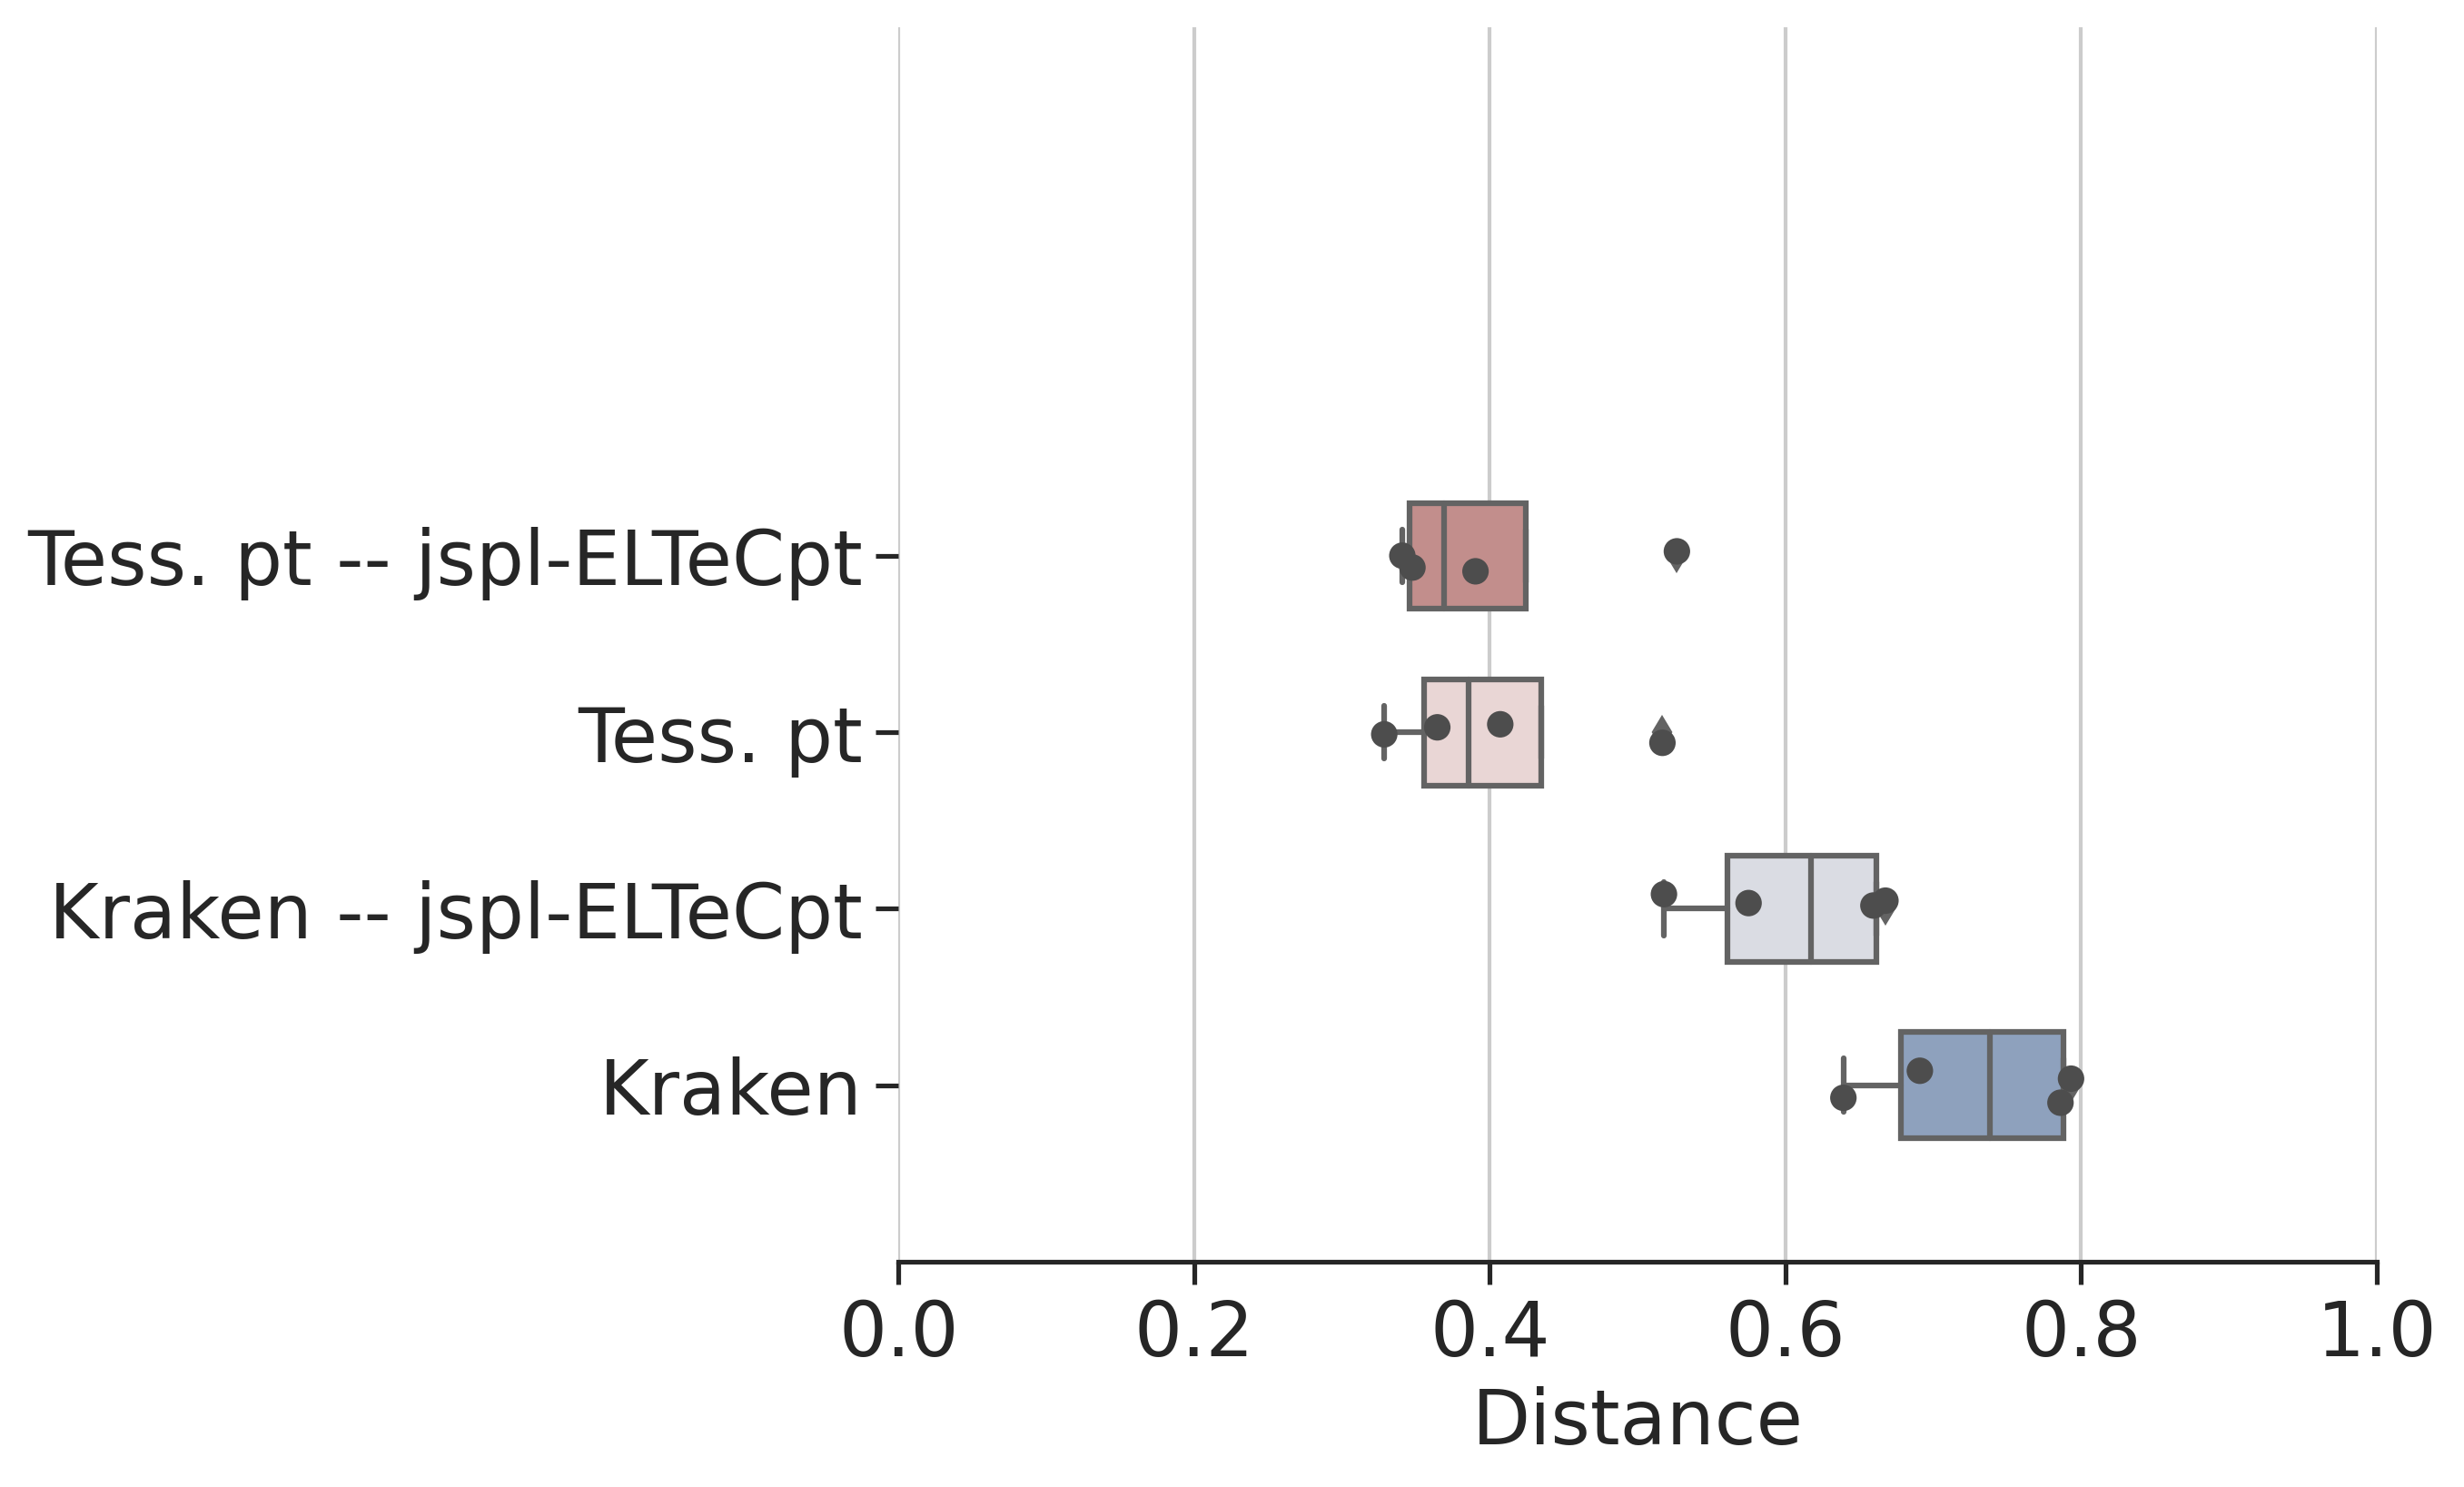
\includegraphics[height=.65\textwidth]{IMAGES/Boite-moustache/ELTeC-Por_REF_jaccard.png} 
        \caption{ELTeC-Por Jaccard}
        \label{fig:ELTeC-Por_REF_jaccard}
   \end{subfigure}
    \begin{subfigure}{0.5\textwidth}
  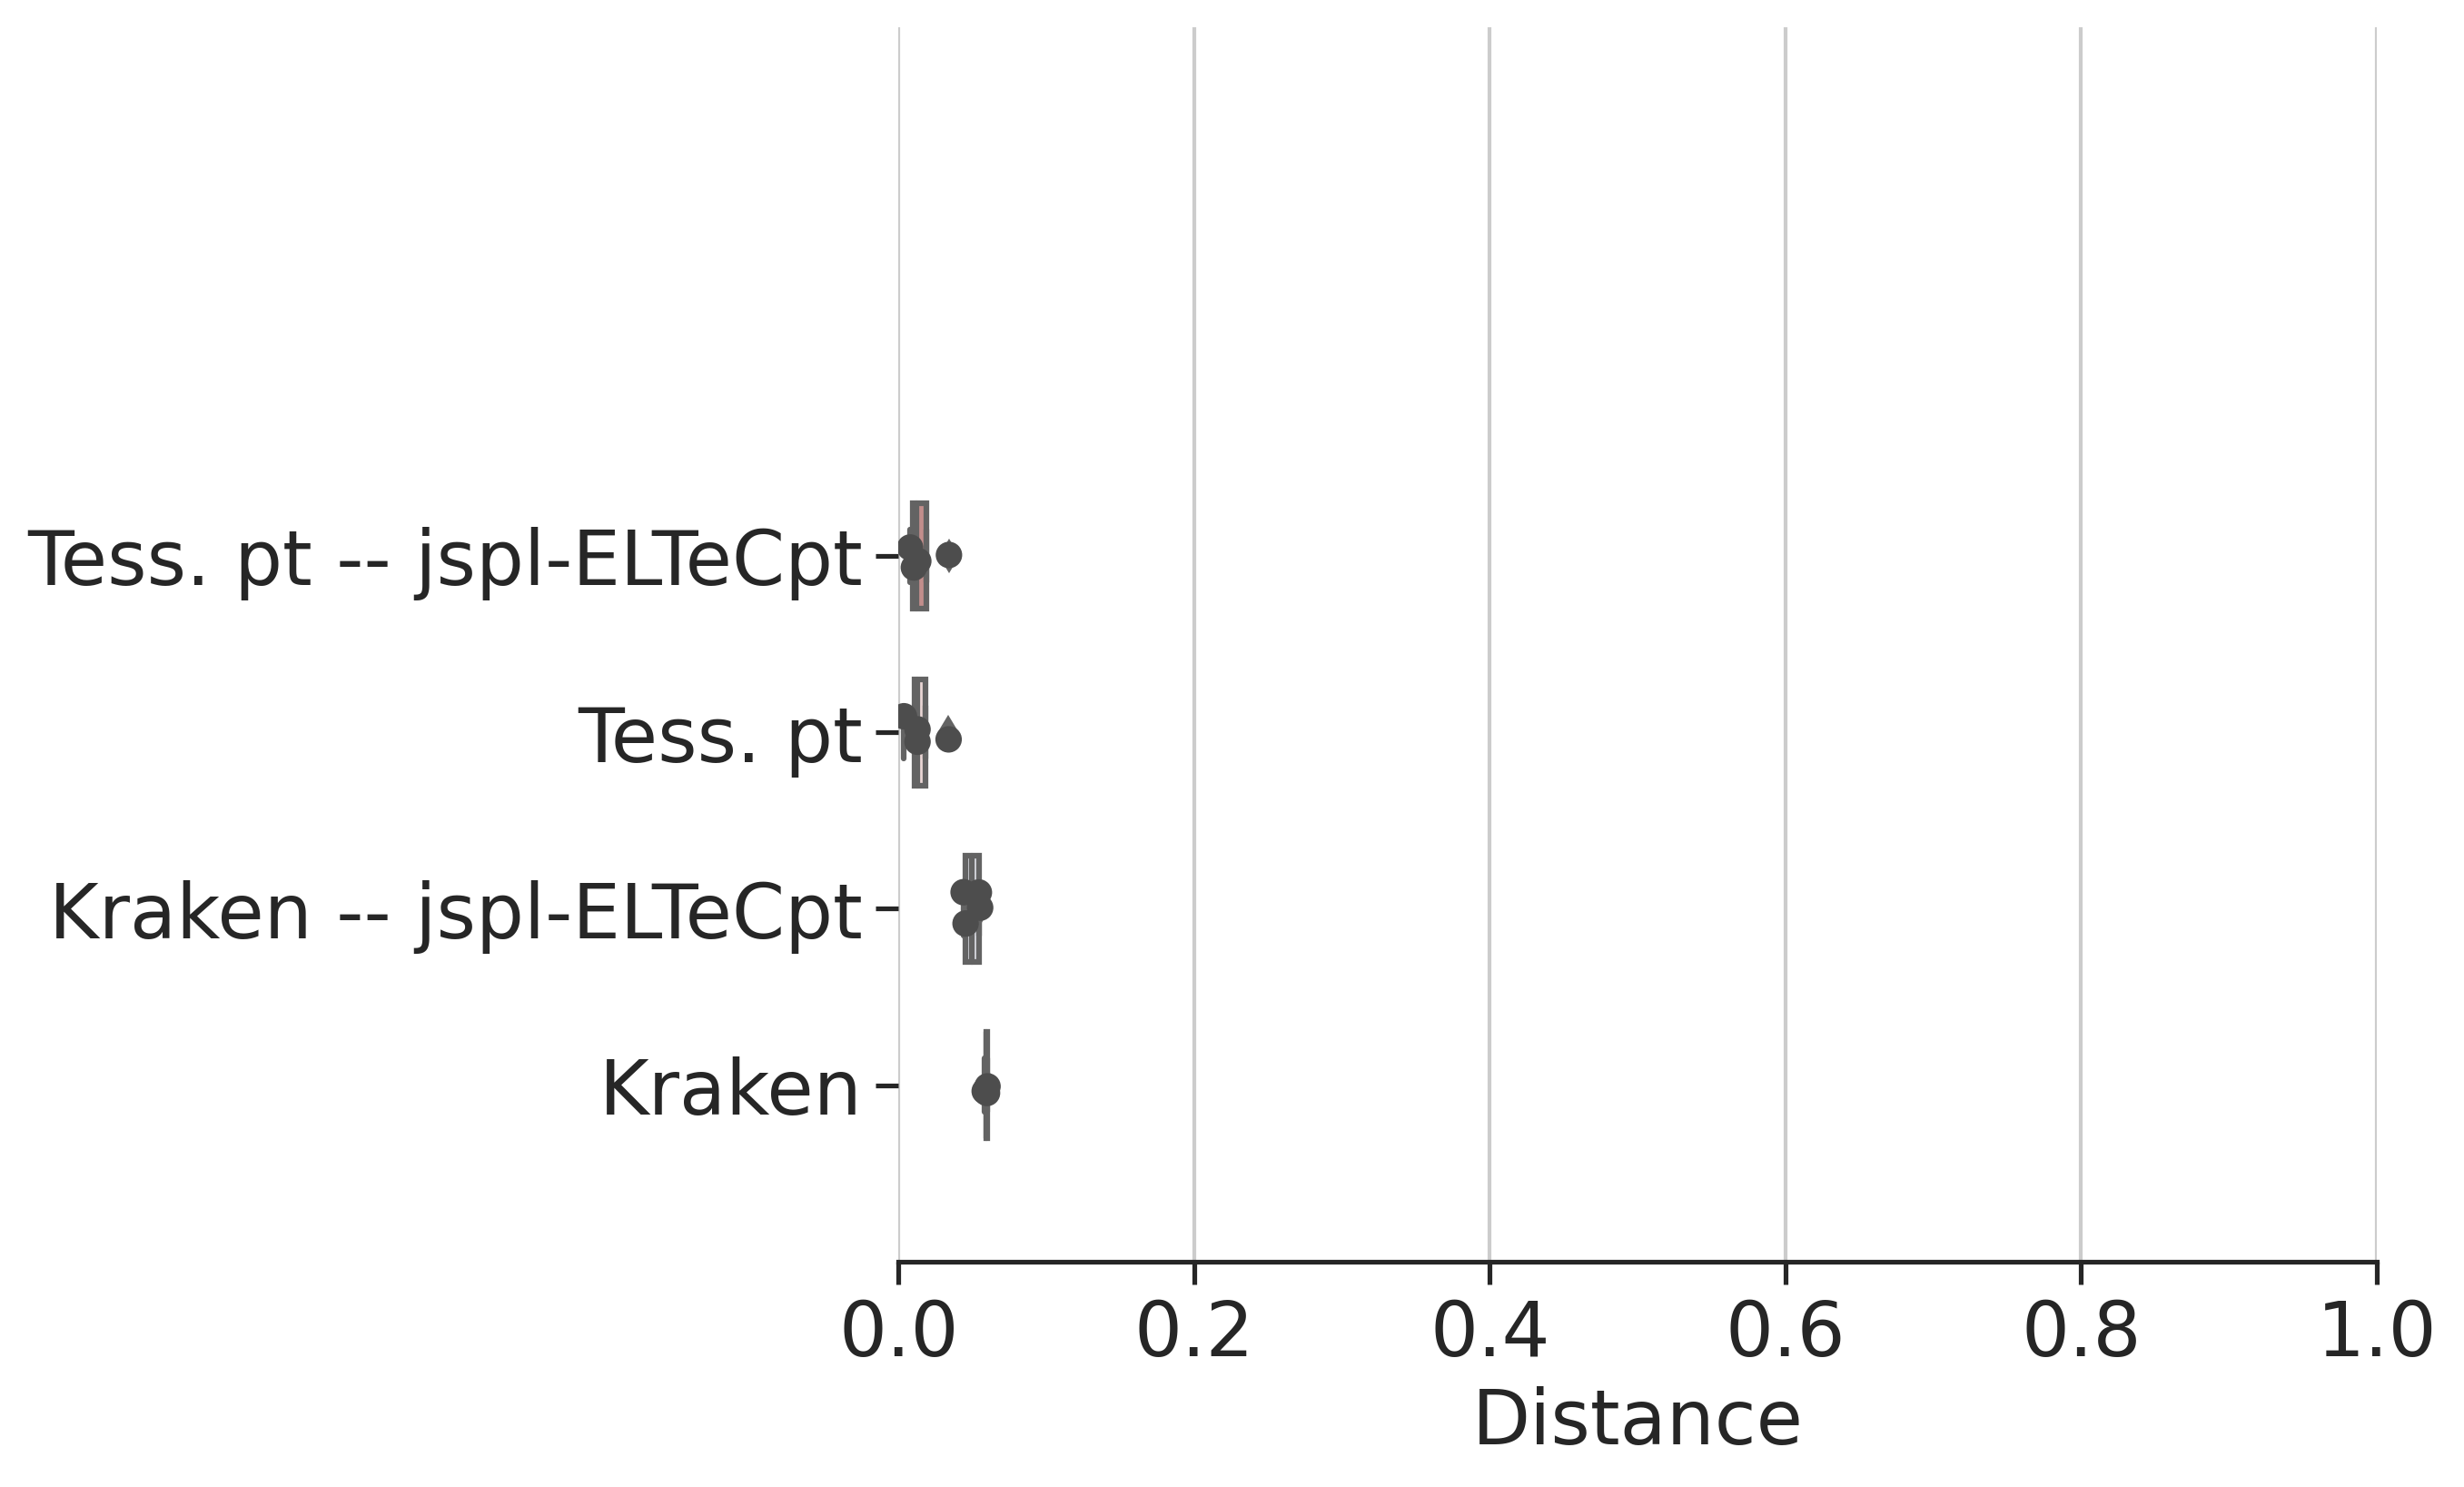
\includegraphics[height=.65\textwidth]{IMAGES/Boite-moustache/ELTeC-Por_REF_cosinus.png} 
        \caption{ELTeC-Por cosinus}
        \label{fig:ELTeC-Por_REF_cosinus}
   \end{subfigure}   
%    \caption{Distances calculées entre les textes de référence et les versions de ROC.}
\label{fig:distance_texte}
%\end{figure}

%%% TODO GL: Alignement des figures boites à moustache
%\begin{figure}
%   \centering
         \begin{subfigure}{0.45\textwidth}
  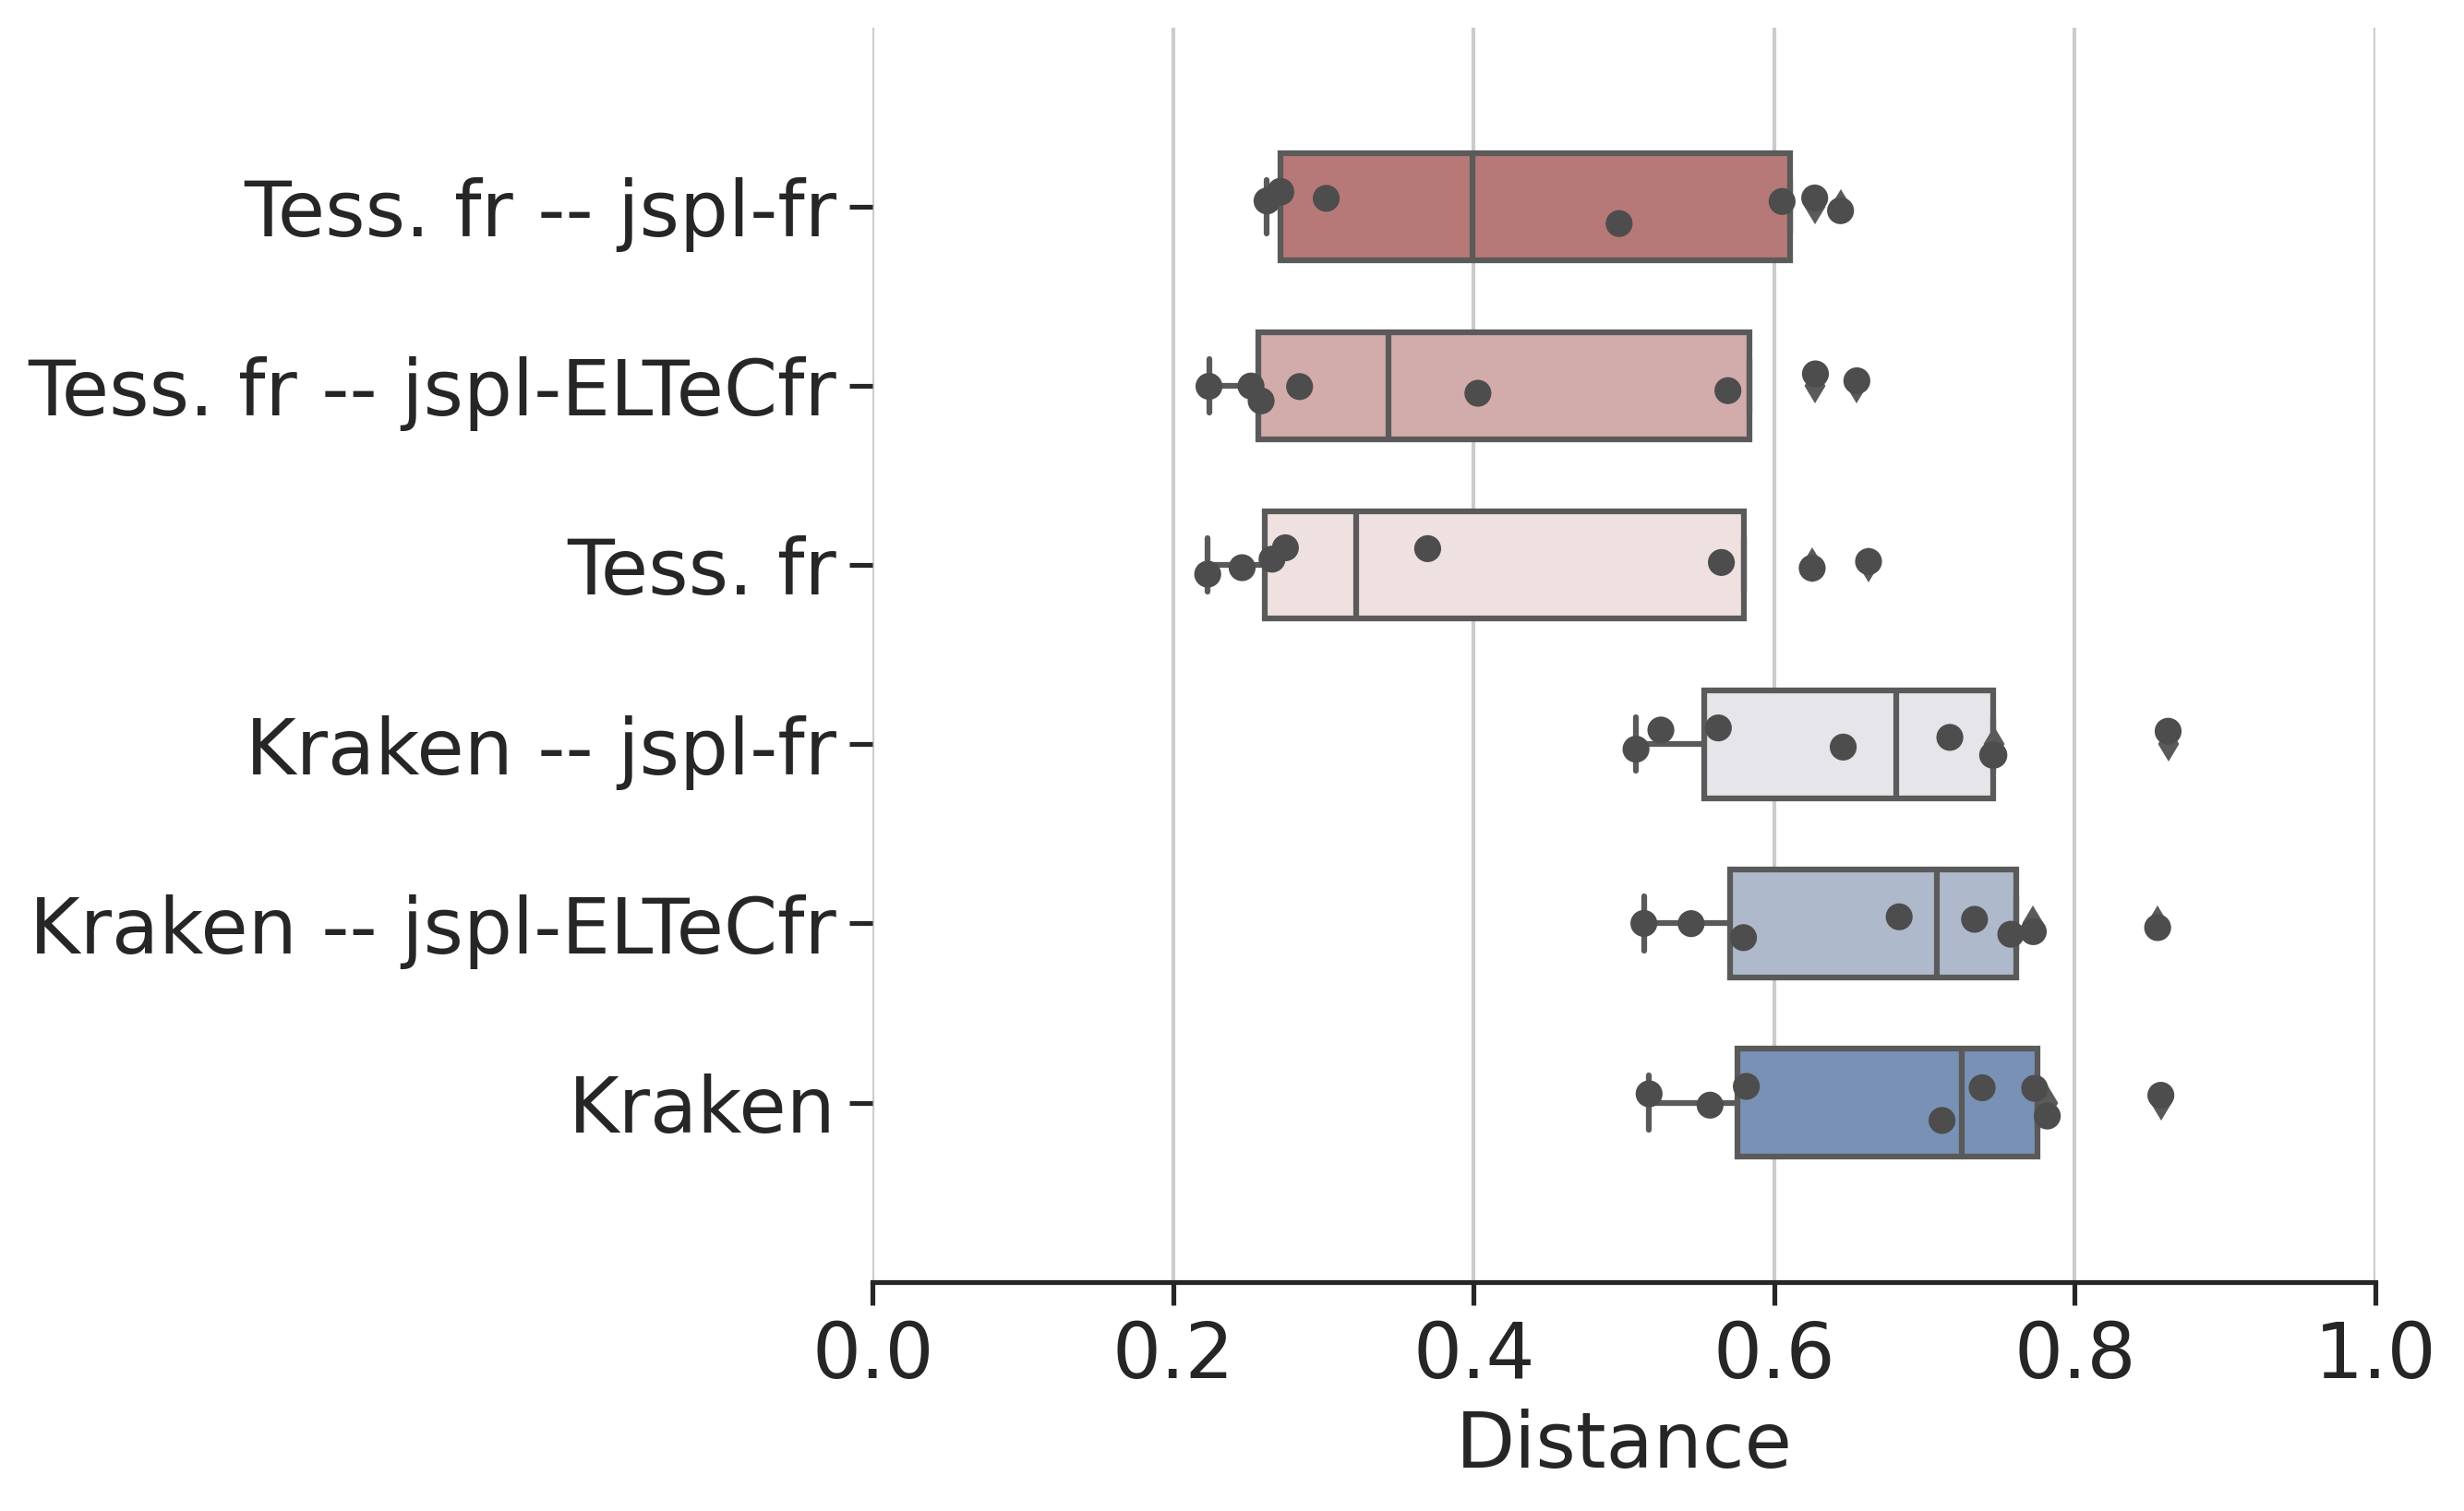
\includegraphics[height=.65\textwidth]{IMAGES/Boite-moustache/TGB_REF_jaccard.png} 
        \caption{TGB Jaccard}
   \end{subfigure}
    \begin{subfigure}{0.5\textwidth}
  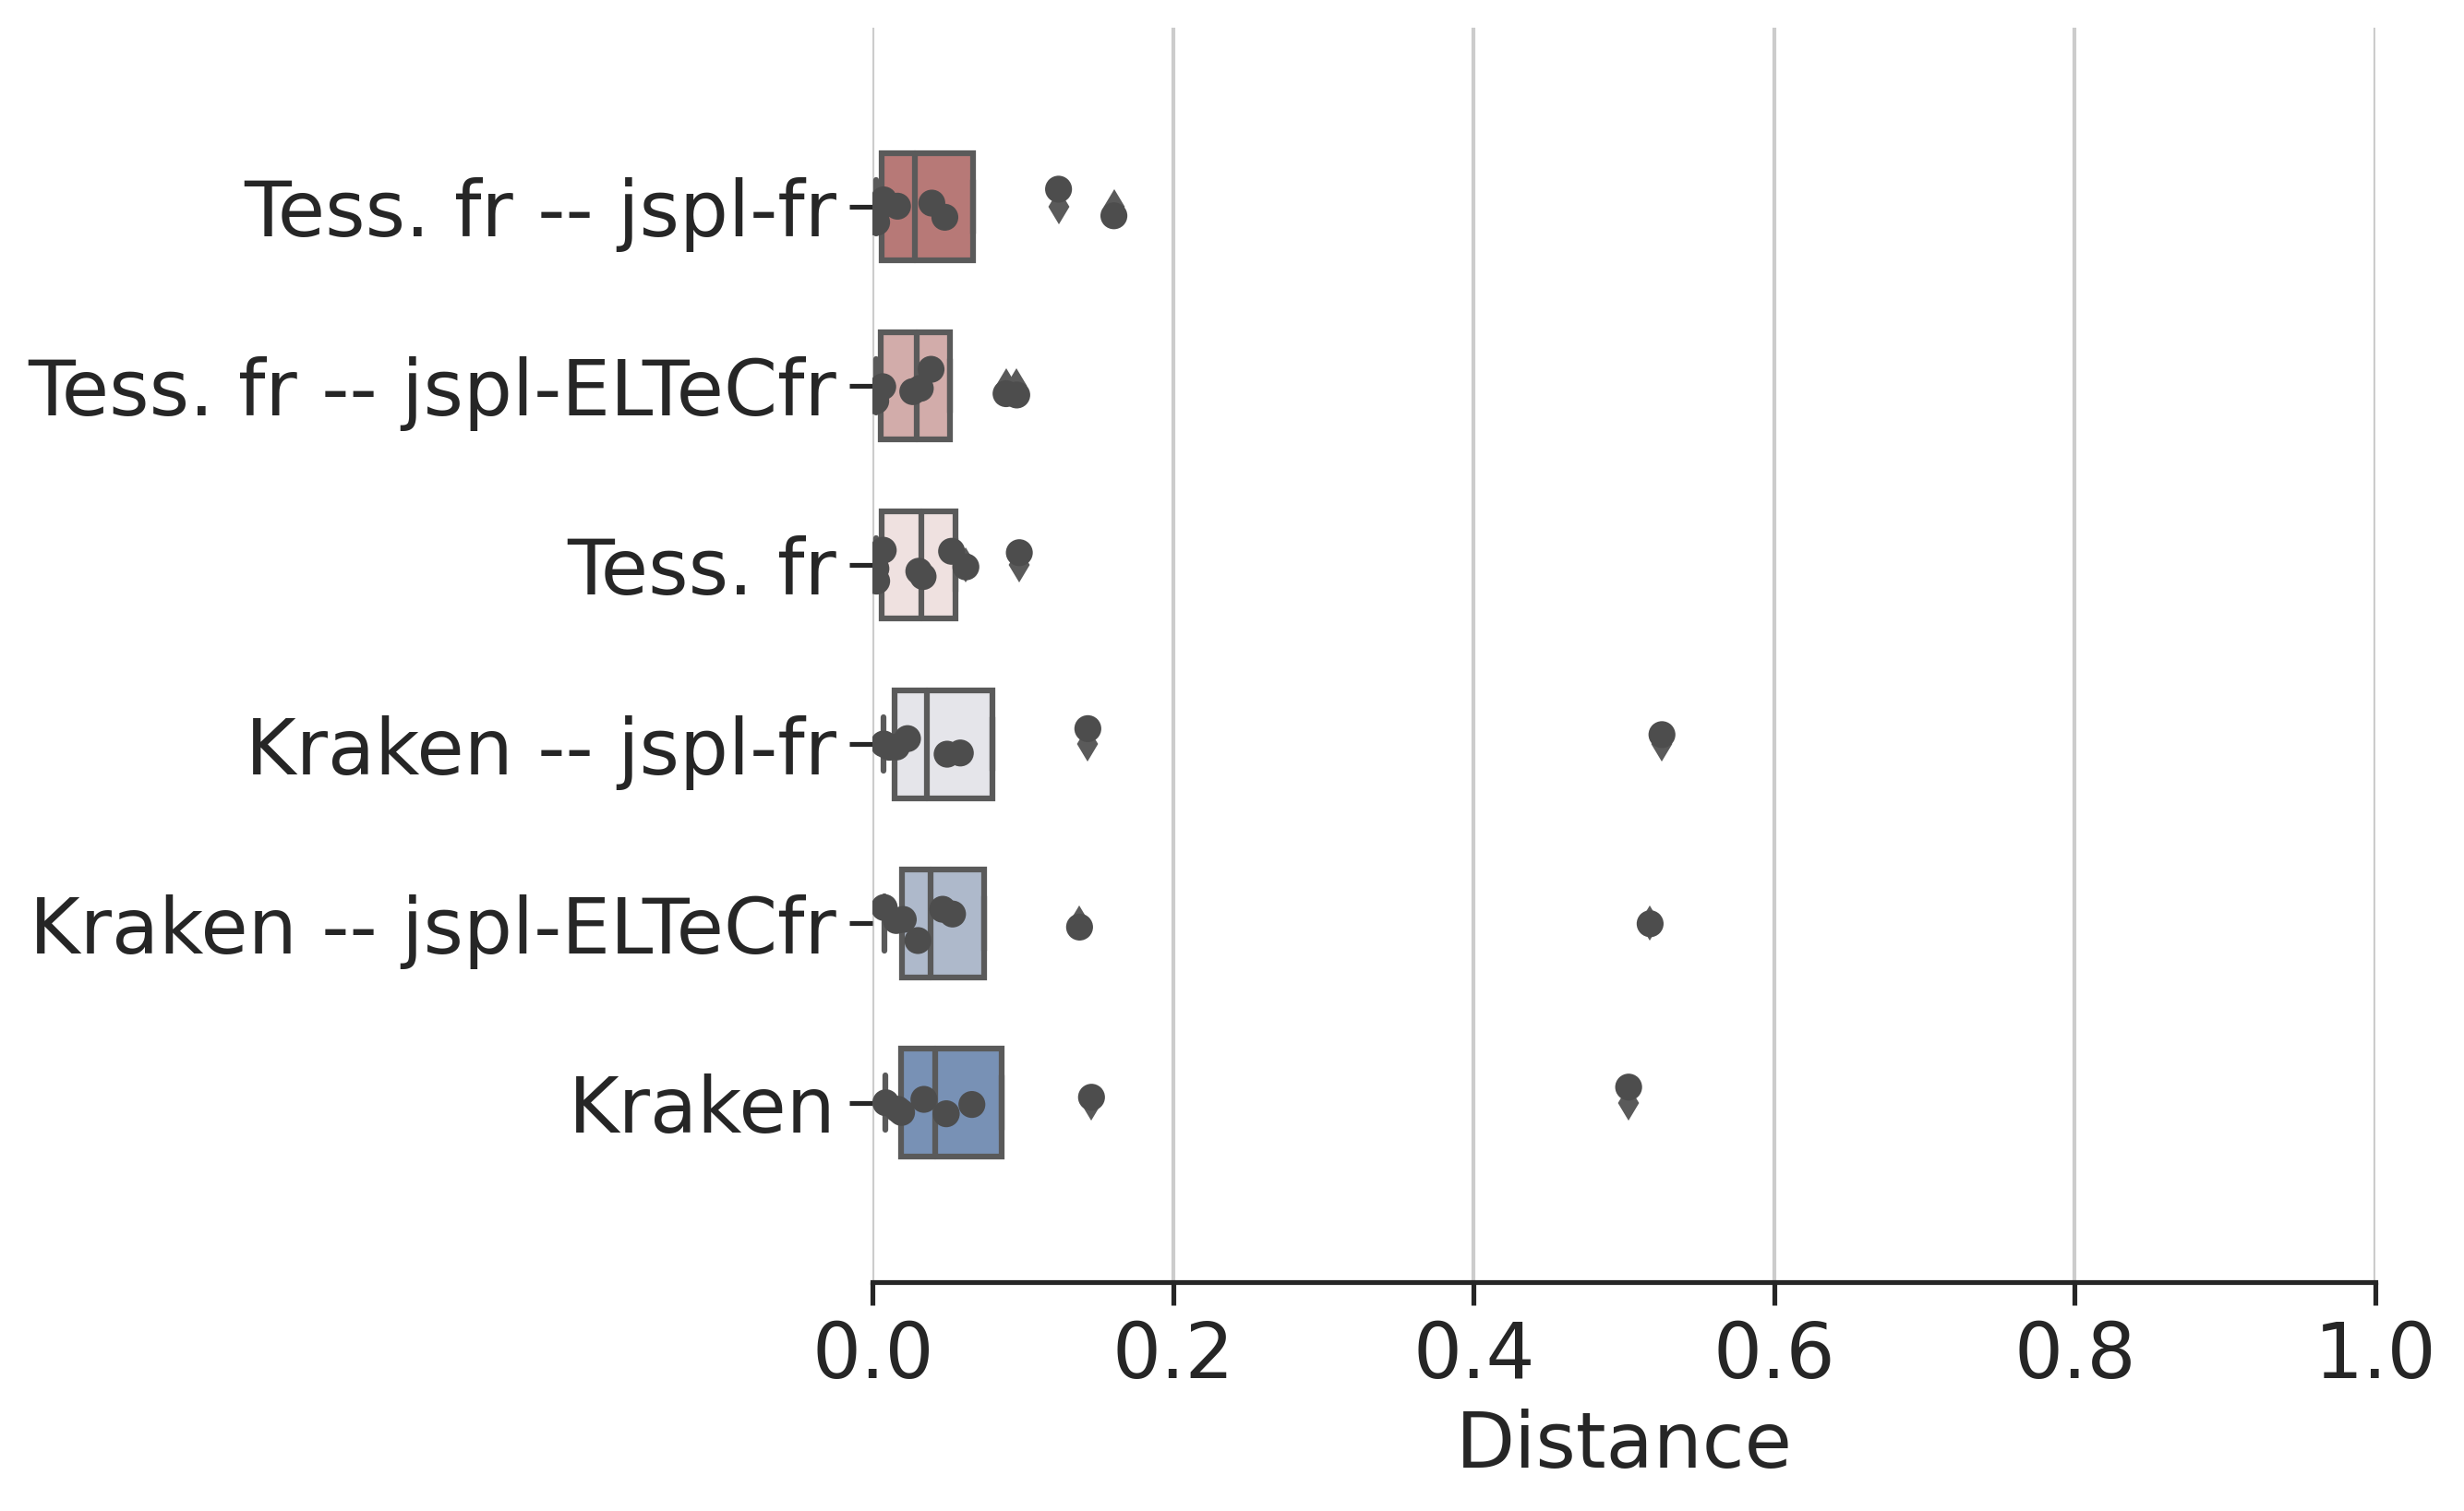
\includegraphics[height=.65\textwidth]{IMAGES/Boite-moustache/TGB_REF_cosinus.png} 
        \caption{TGB cosinus}
   \end{subfigure}
   
    \caption{Distances calculées entre les textes de référence et les versions de ROC.}
    \label{fig:distances_ref_roc}
\end{figure}

Les figures \ref{fig:distances_ref_roc} et \ref{fig:Cosinus-spacy-lg} montrent les résultats obtenus en comparant les sorties de REN obtenues sur les textes de référence et celles des différentes configurations évaluées (tableau \ref{tab:config}). Pour lire ces figures, il faut noter que plus la boîte est proche de zéro, plus les sorties comparées sont similaires.
Après une observation des différentes mesures de distance présentées pour chaque sous-corpus évalué, on note l'écart constant et considérable entre les résultats de Jaccard et cosinus. Les résutats pour Jaccard sont souvent proches de 1, tandis que ceux de cosinus sont proches de 0 pour les comparaisons des mêmes configurations. Il semble que la métrique cosinus sous-estime la distance entre les résultats pour les configurations de ROC et celles de référence. 

\begin{figure}[h!]

    \begin{subfigure}{0.45\textwidth}
  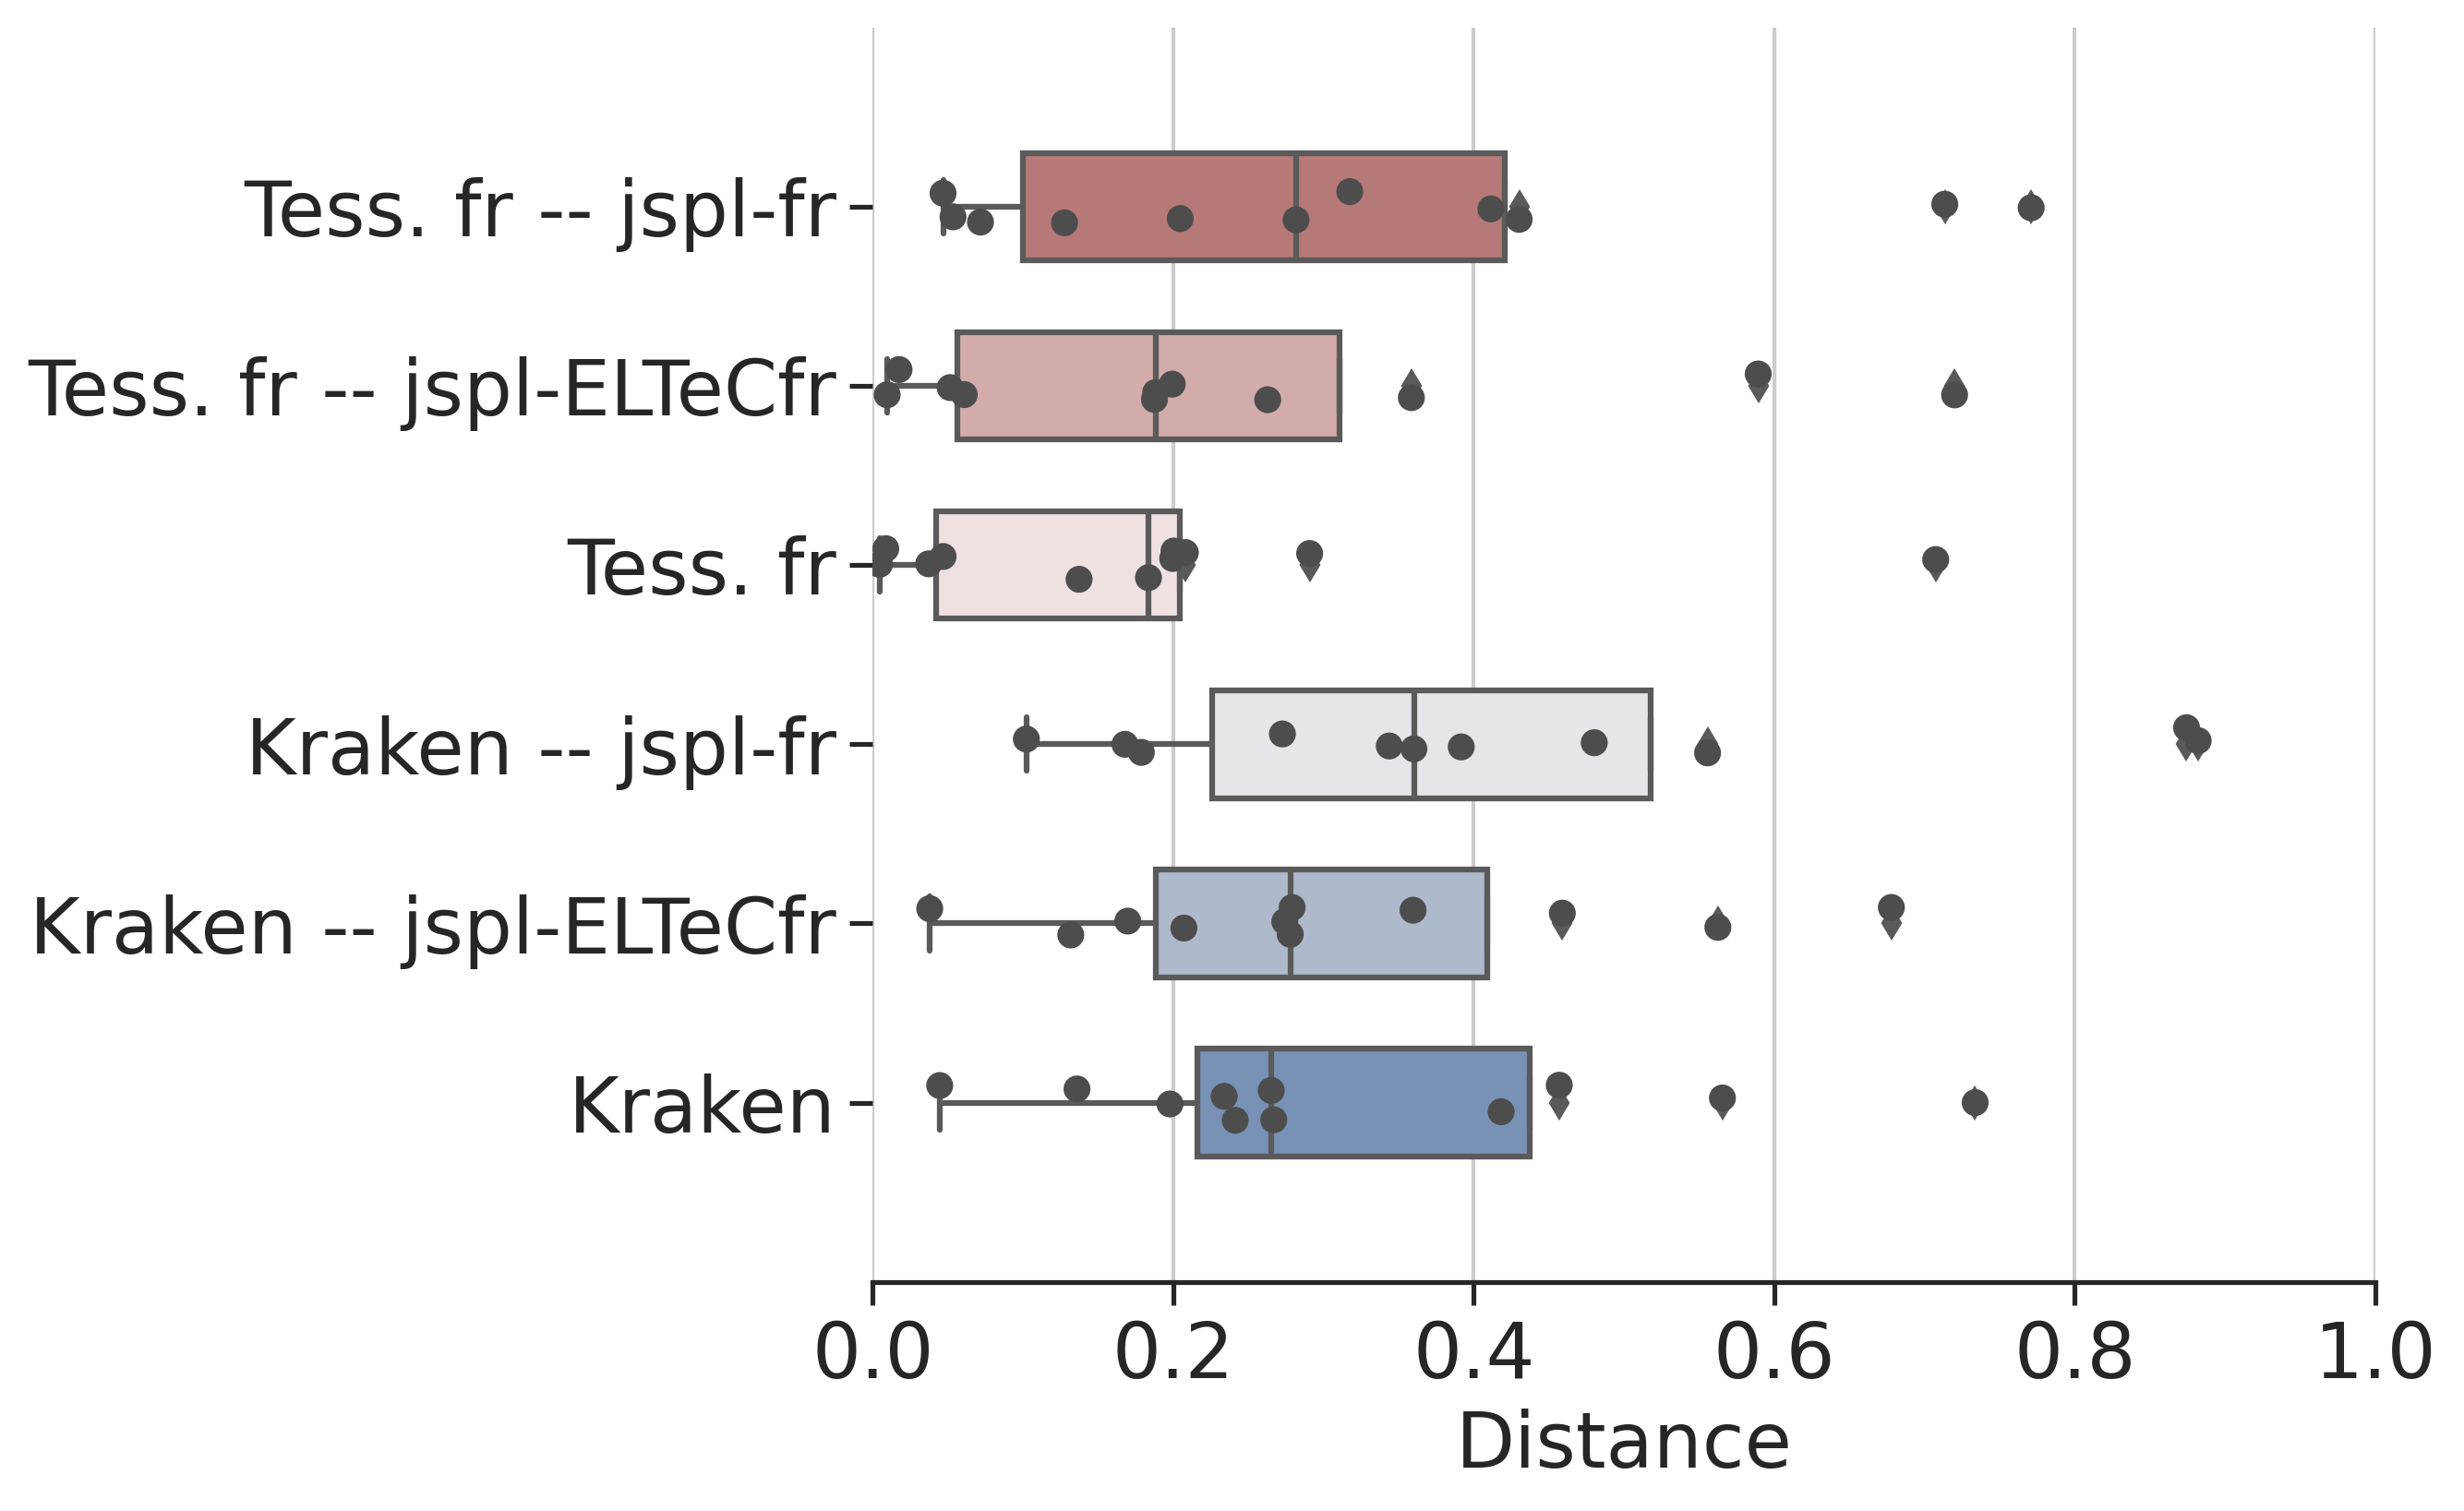
\includegraphics[height=.65\textwidth]{IMAGES/Boite-moustache/ELTeC-Fra_spacy3.5.1_cosinus.png} 
        \caption{ELTeC-Fra \texttt{spaCy} cosinus}
   \end{subfigure}
 \begin{subfigure}{0.45\textwidth}
  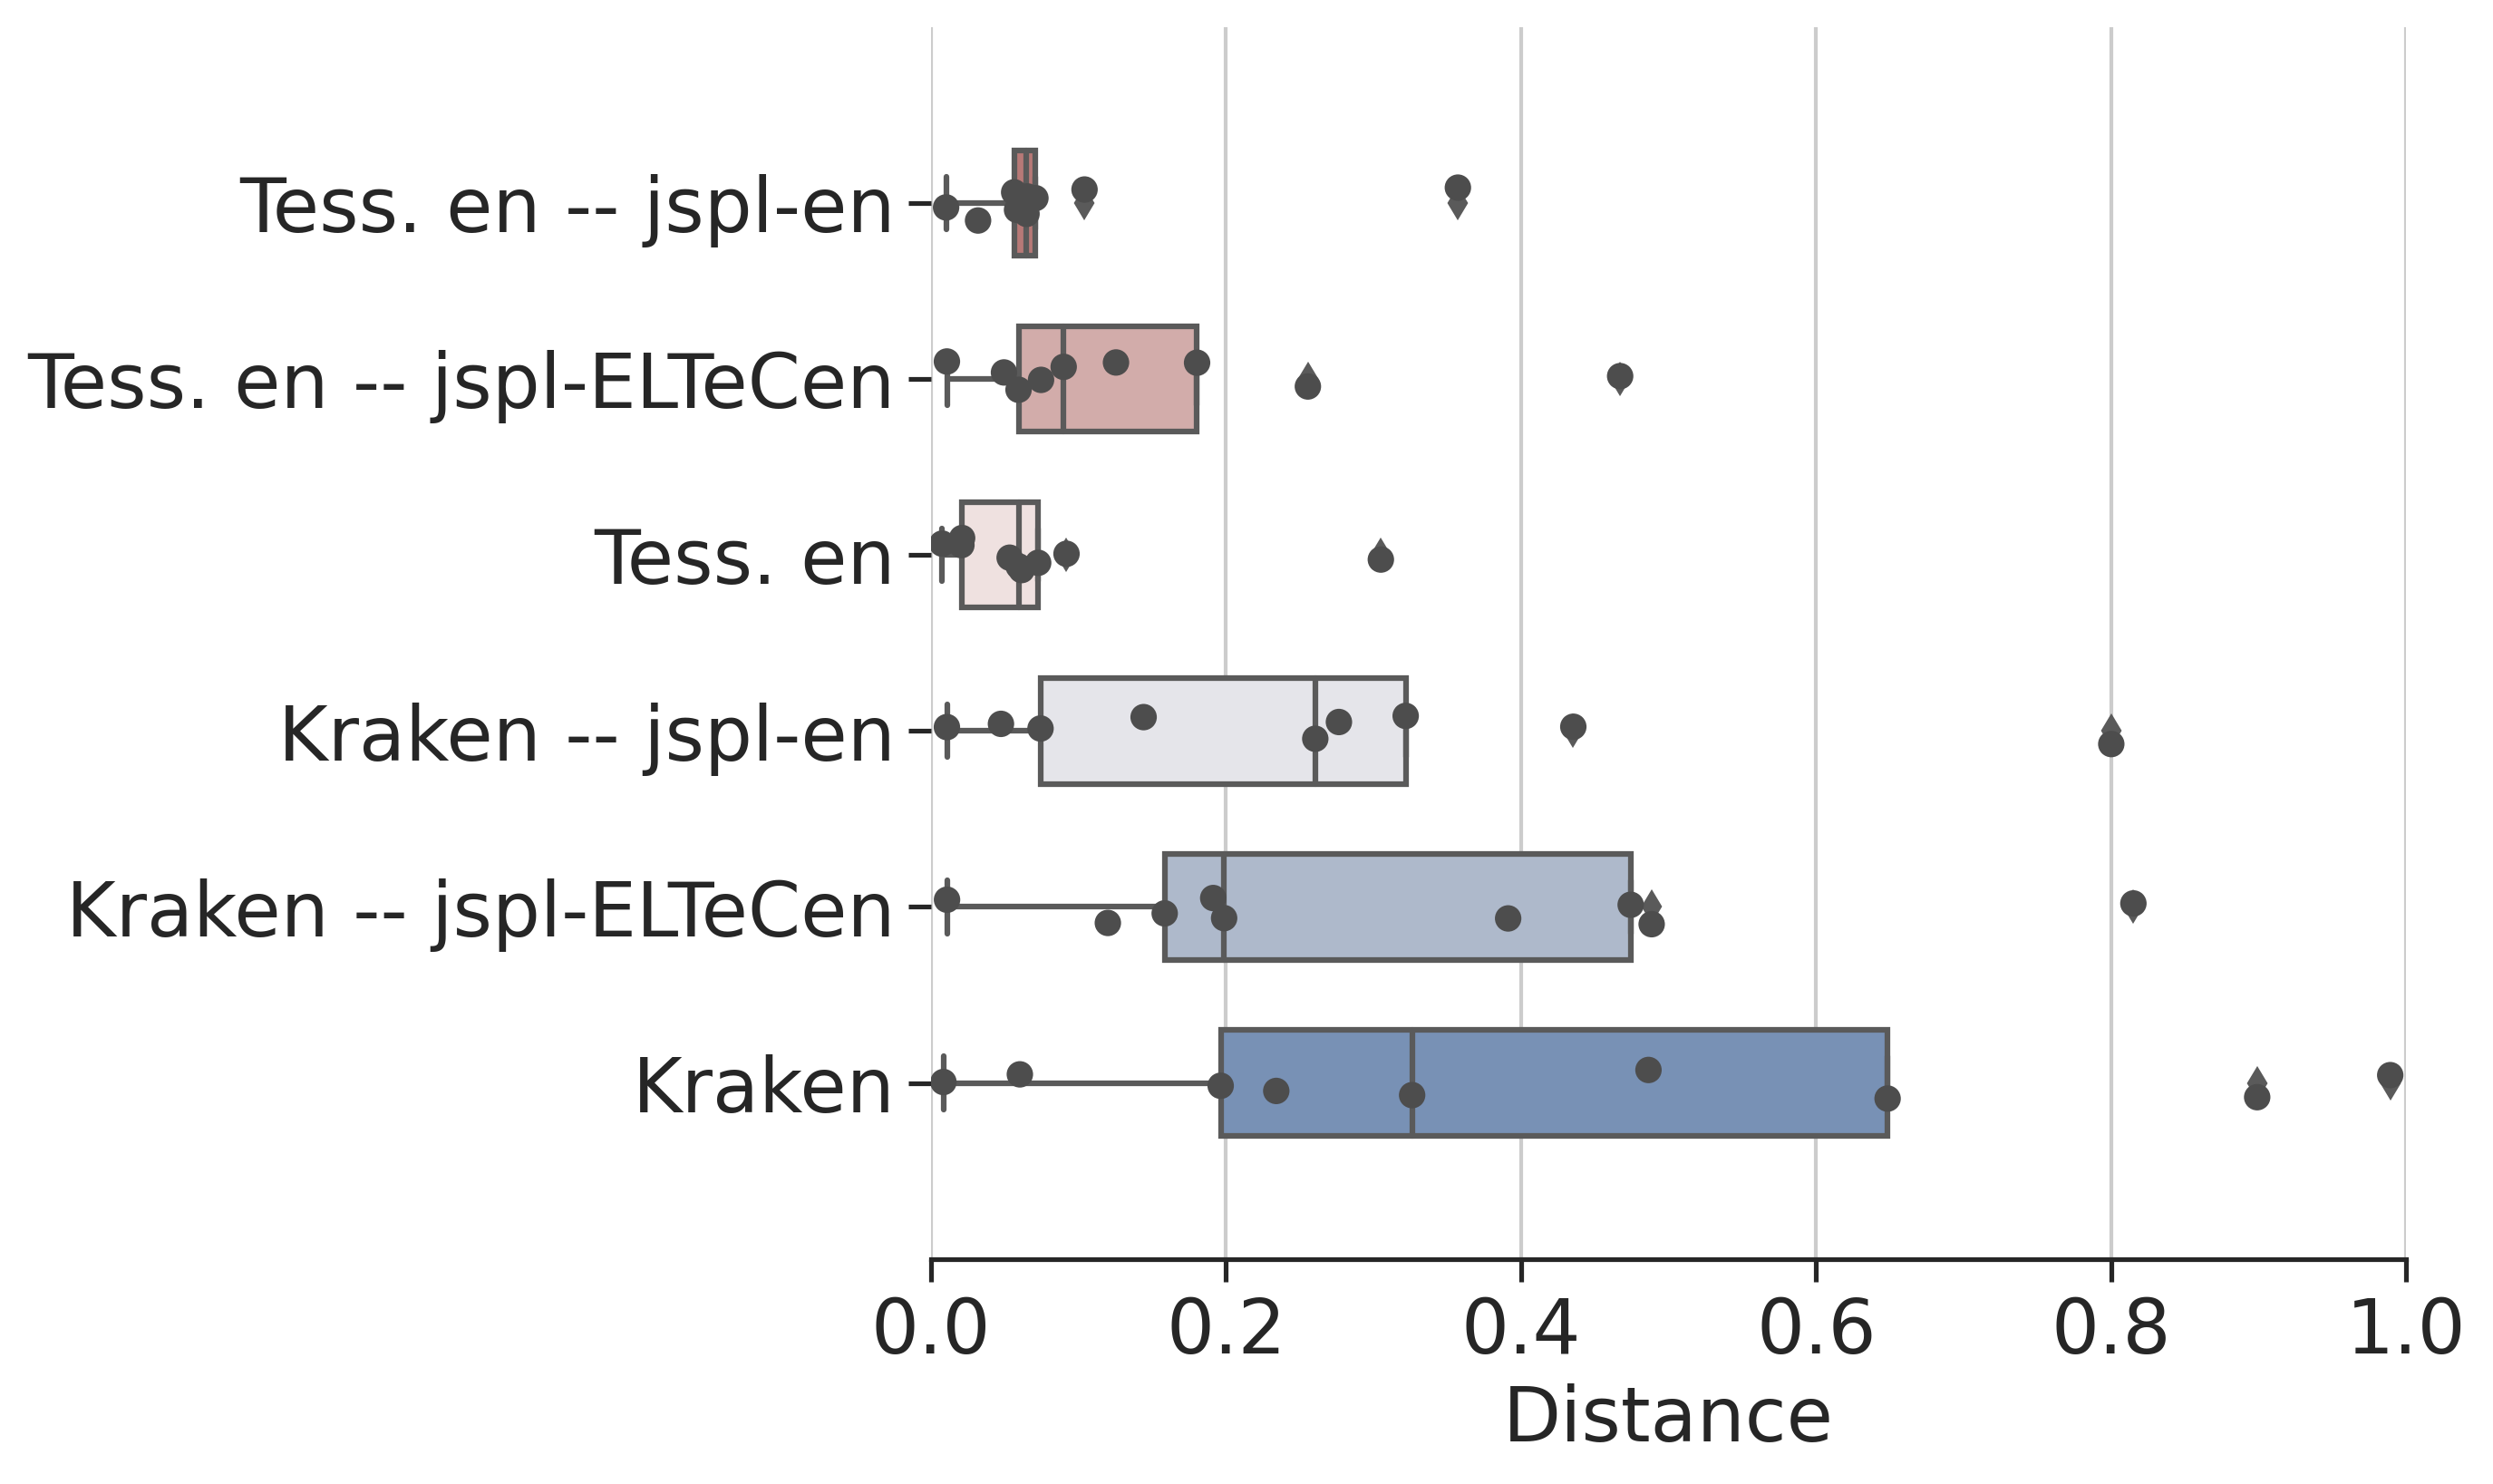
\includegraphics[height=.65\textwidth]{IMAGES/Boite-moustache/ELTeC-Eng_spacy3.5.1_cosinus.png}
        \caption{ELTeC-Eng \texttt{spaCy} cosinus}
   \end{subfigure}
    \begin{subfigure}{0.5\textwidth}
  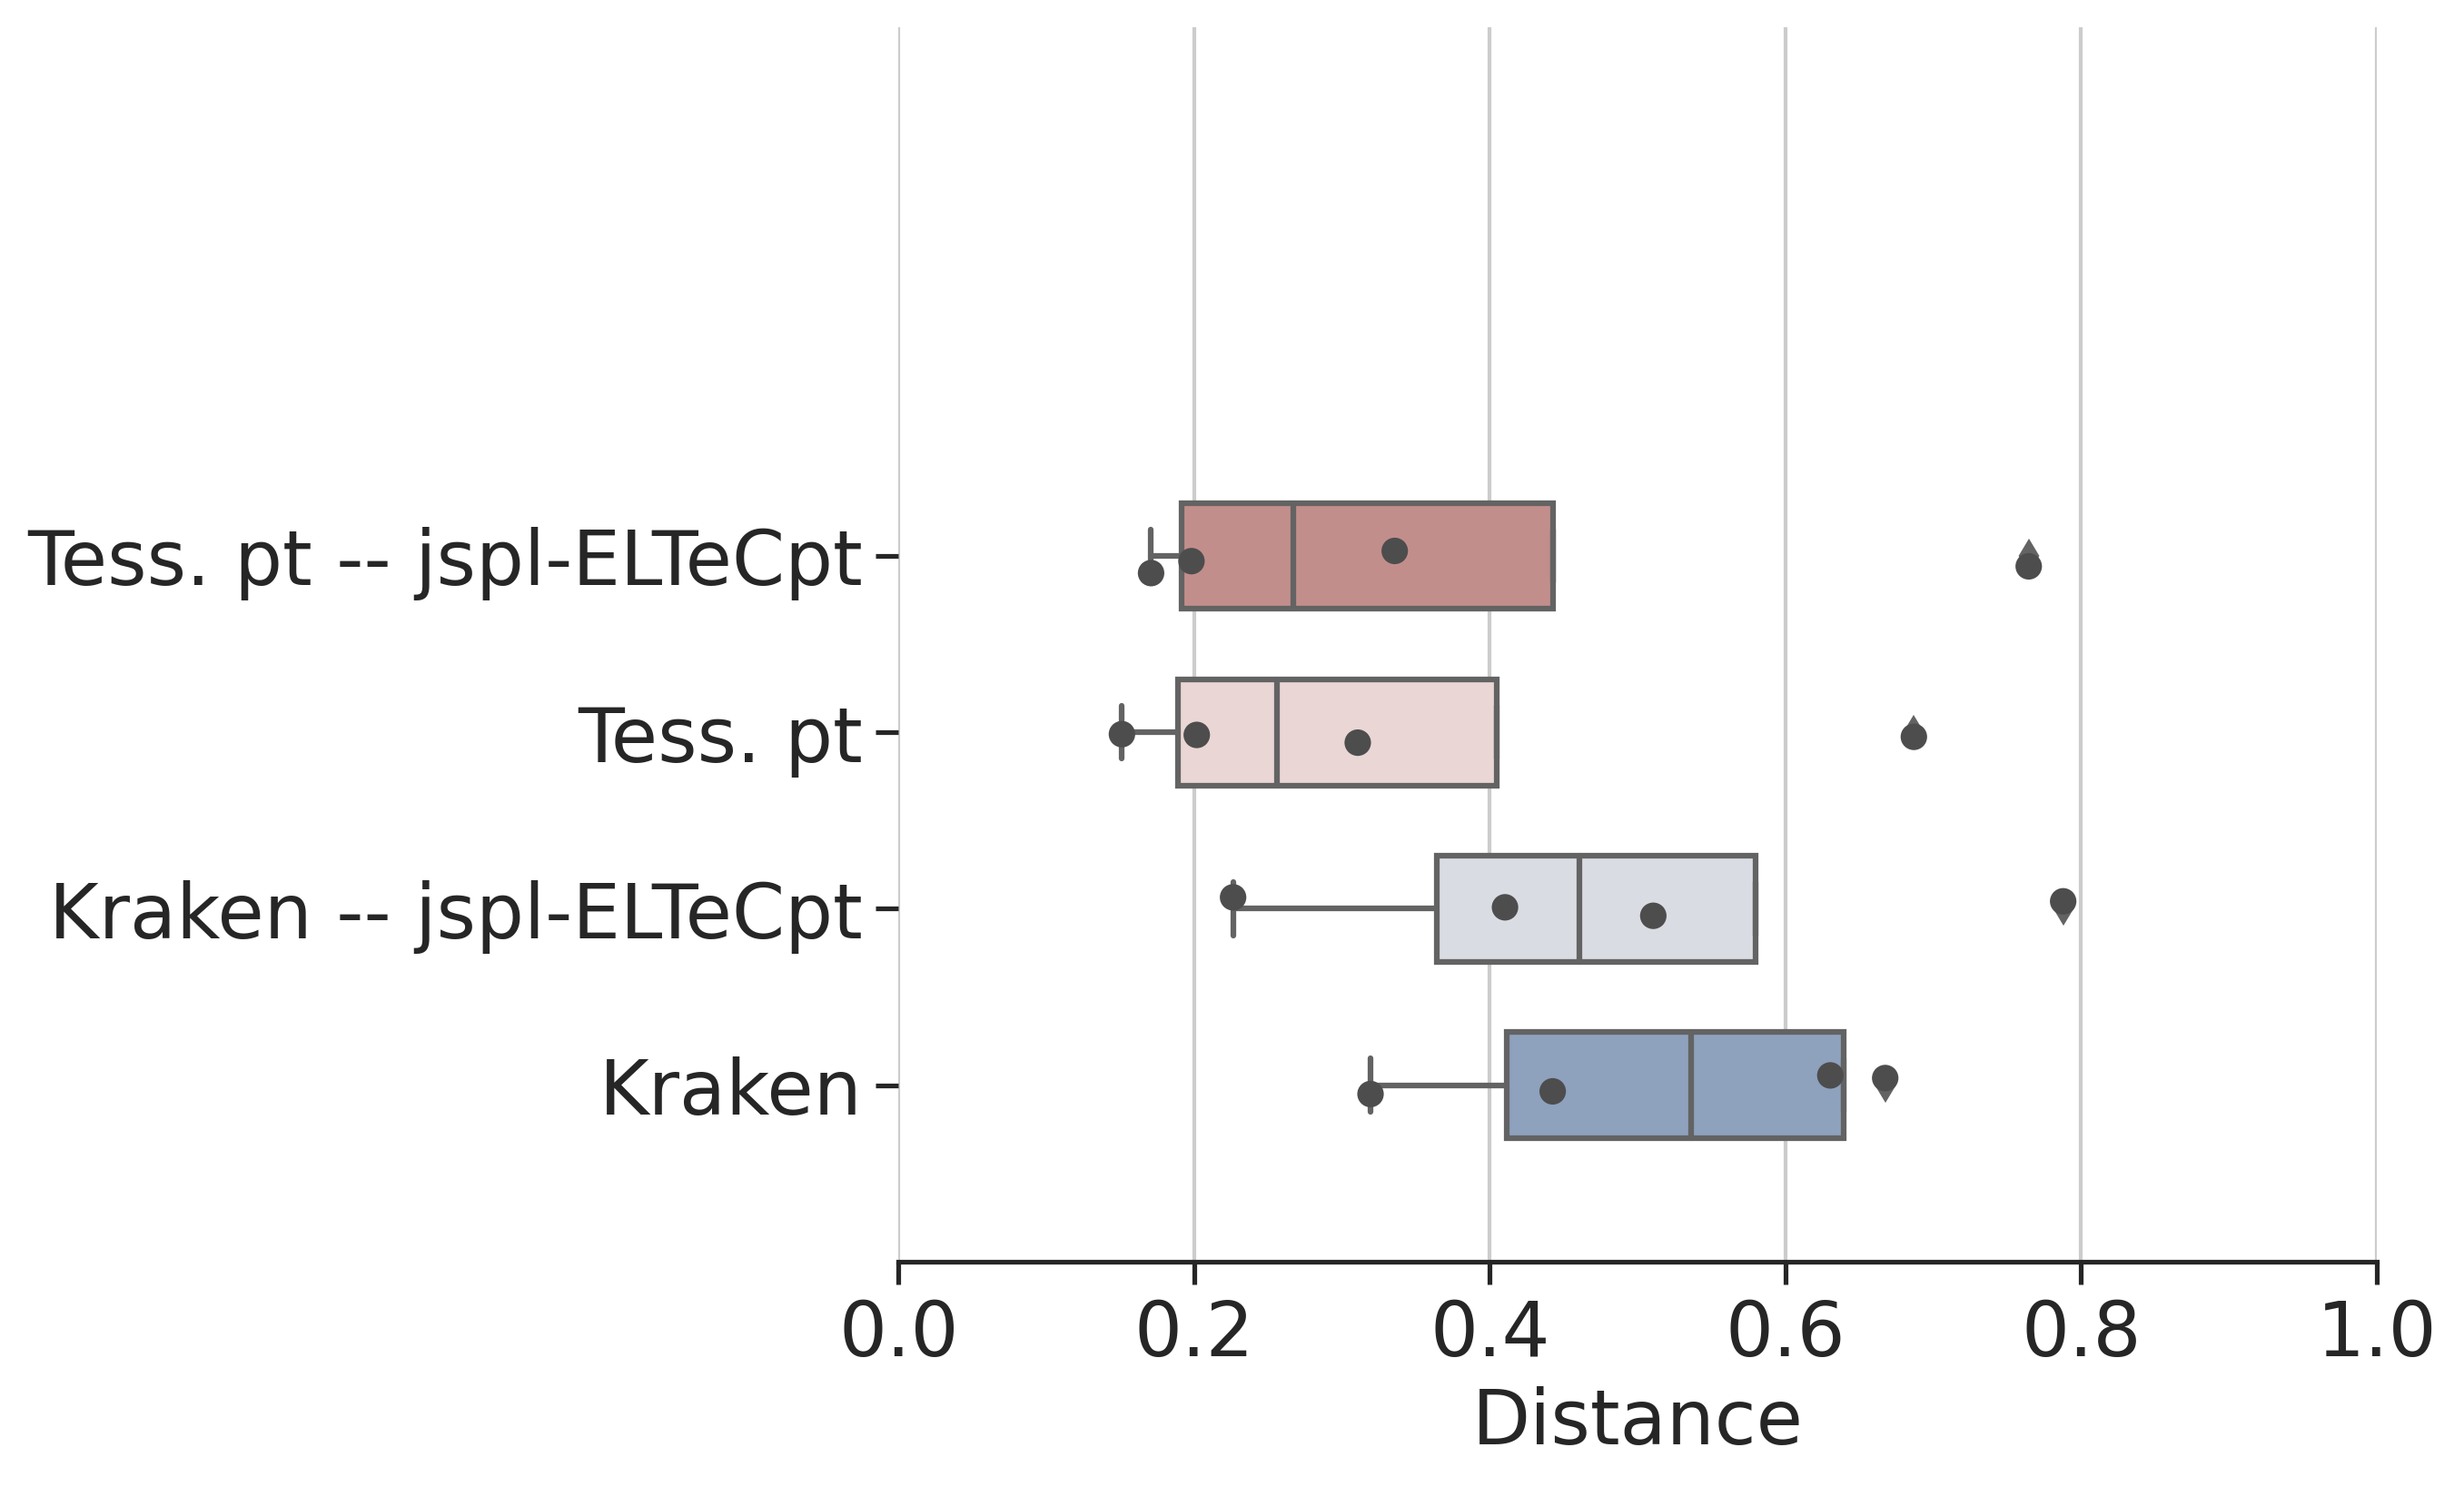
\includegraphics[height=.65\textwidth]{IMAGES/Boite-moustache/ELTeC-Por_spaCy3.5.1_cosinus.png} 
        \caption{ELTeC-Por \texttt{spaCy} cosinus} 
         \label{fig:ELTeC-Por-spaCy-cosinus}
   \end{subfigure}
     \begin{subfigure}{0.5\textwidth}
  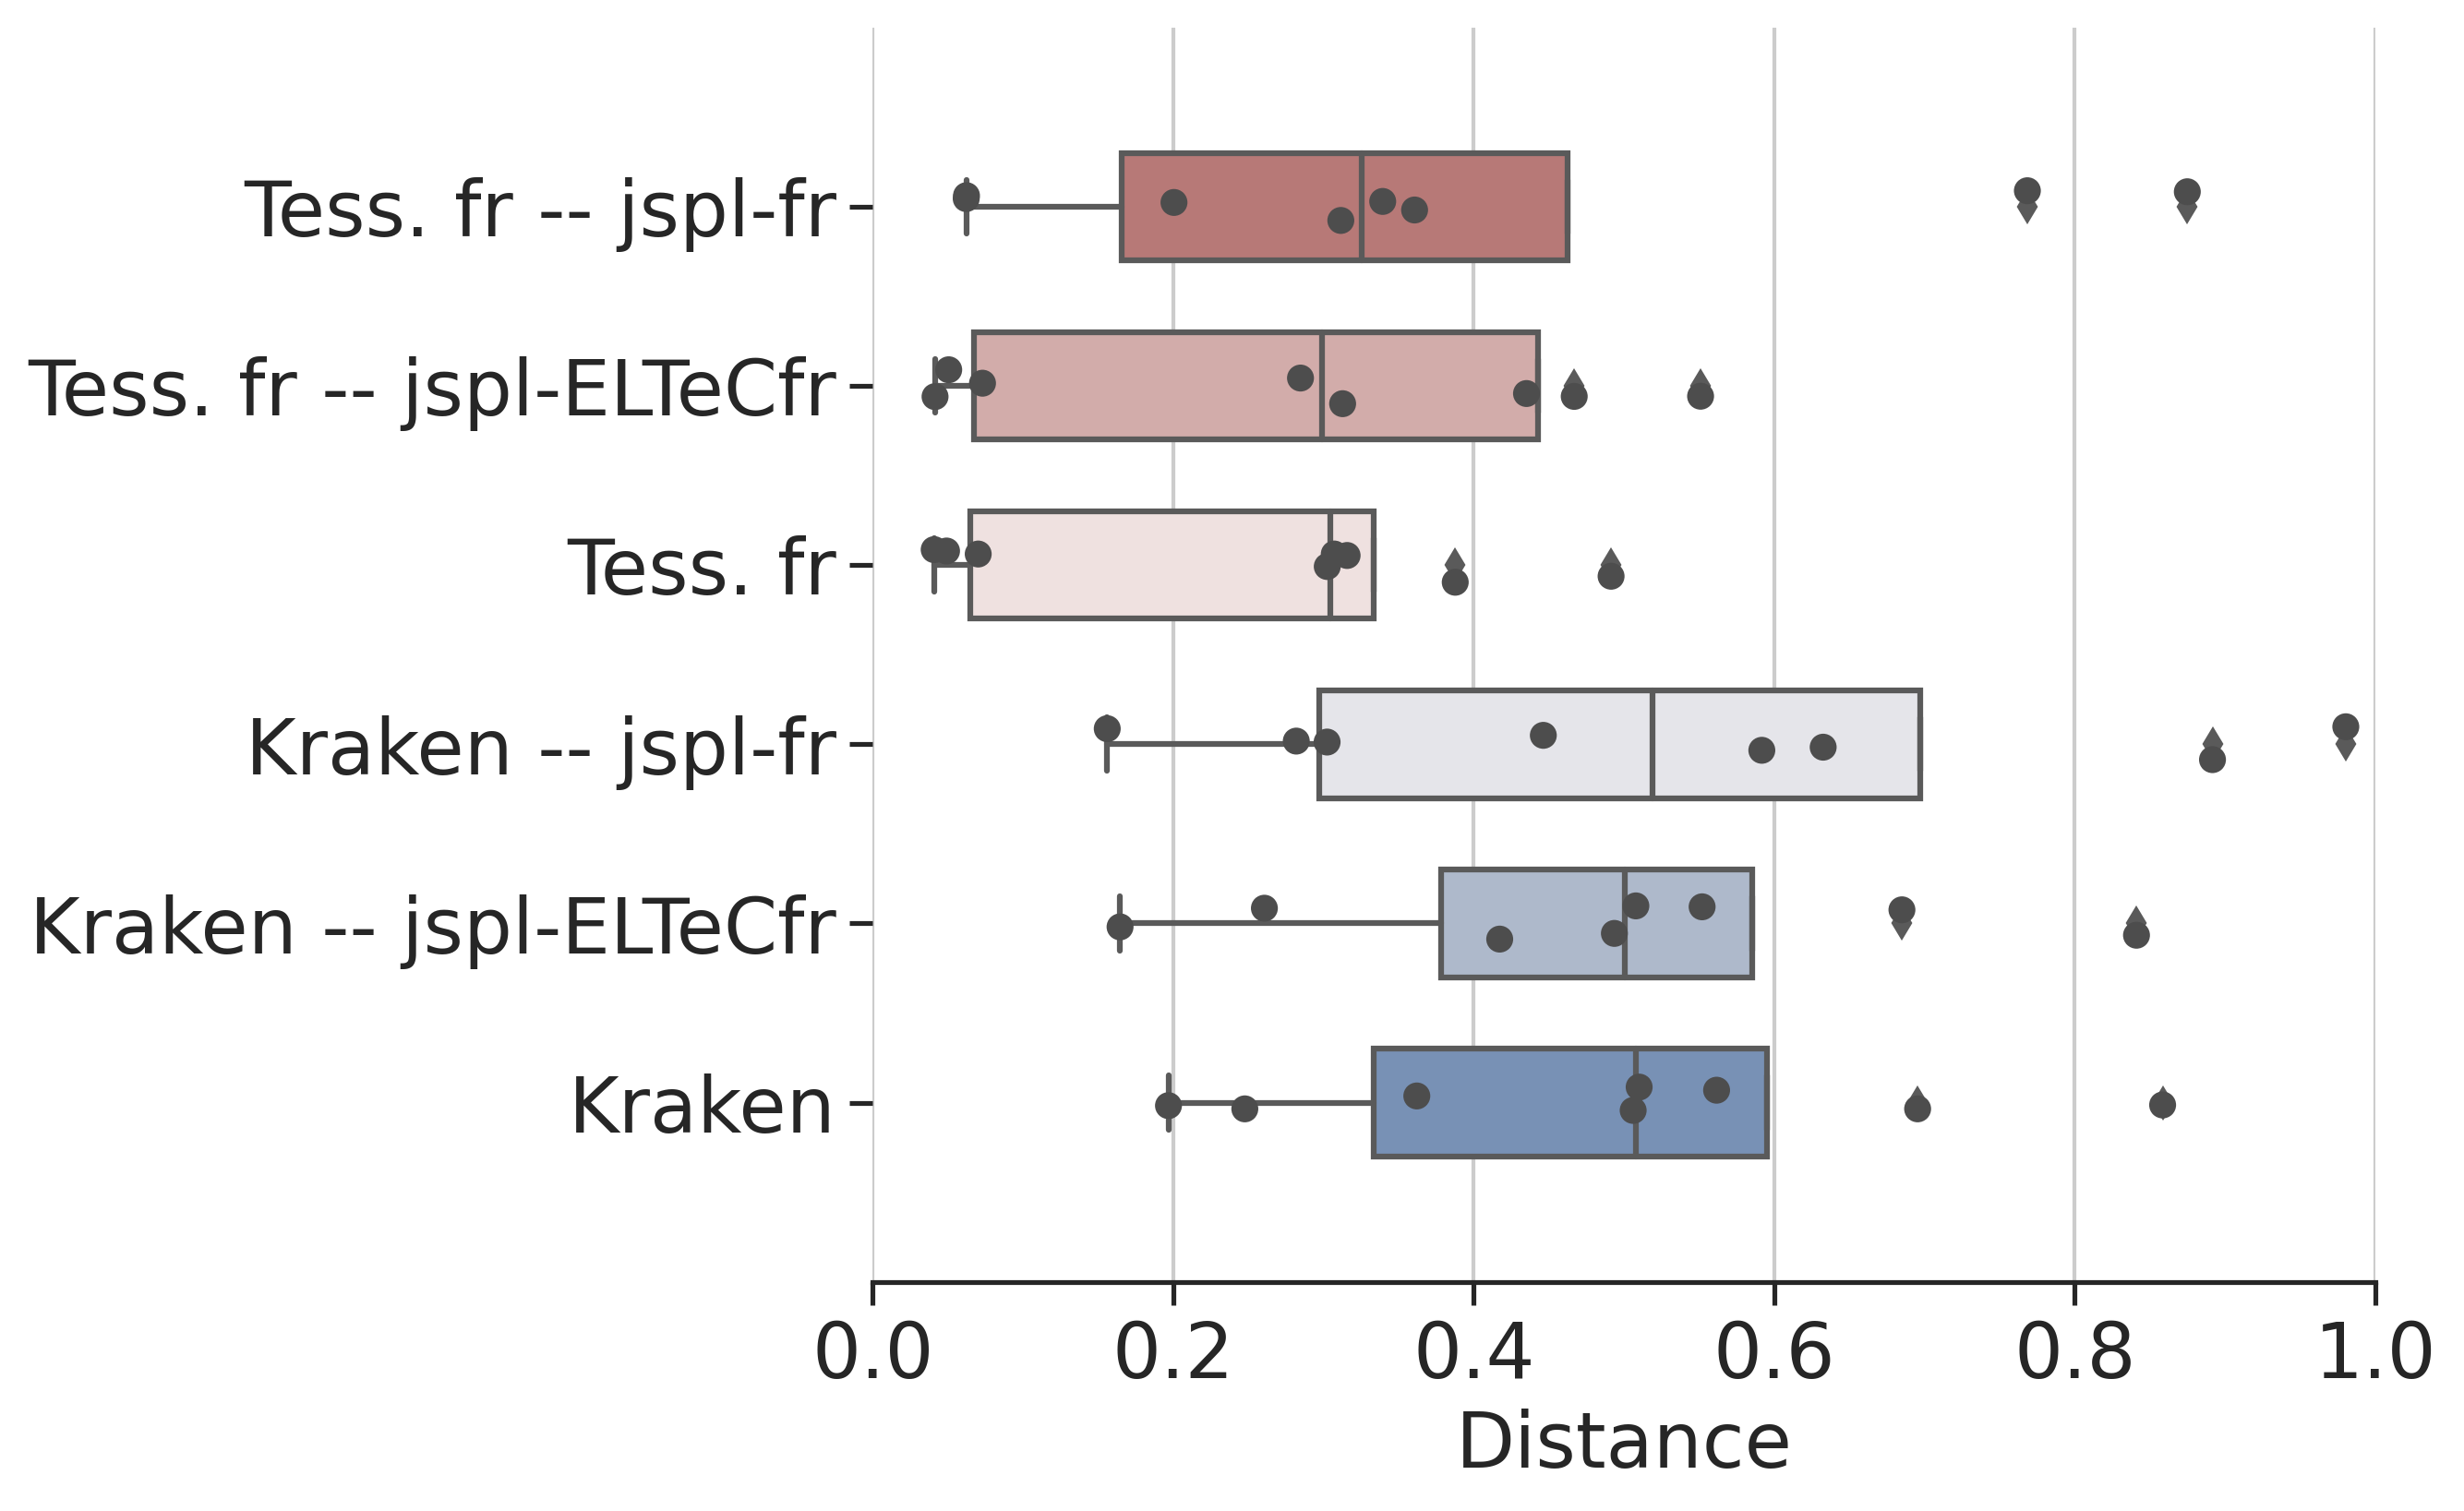
\includegraphics[height=.65\textwidth]{IMAGES/Boite-moustache/TGB_spaCy3.5.1_cosinus.png} 
        \caption{TGB \texttt{spaCy} cosinus}
   \end{subfigure}
    \caption{Distance Cosinus pour \texttt{spaCy\_lg} sur chaque sous-corpus globalement.}
%    \label{fig:Cosinus-spacy-lg-stanza}
\label{fig:Cosinus-spacy-lg}
\end{figure}


Pour préciser notre réflexion s'appuyant sur la lecture des figures \ref{fig:distances_ref_roc} et \ref{fig:Cosinus-spacy-lg},
% et \ref{fig:Cosinus-spacy-lg-stanza} 
nous avons procédé à la lecture des figures obtenues pour chacun des autres corpus et consulté manuellement les résultats effectifs de REN. Finalement, cette différence entre les résultats de Jaccard et cosinus pourrait s'expliquer par le fait que la première mesure prend en compte le vocabulaire, alors que la seconde s'intéresse au nombre d'occurrences d'une EN. Concrètement, cela signifie pour la distance de Jaccard que si le vocabulaire entre les sorties de deux ensemble pour les configurations comparées est très différent, le résultat est proche de 1. 
En revanche, les résultats pour la mesure cosinus dépendraient du nombre d'occurences de chaque EN dans les groupes comparés. Autrement dit, s'il y a beaucoup d'occurrences d'une EN dans une des configurations comparée mais qu'elle n'apparaît pas en même quantité dans les résultats de la seconde configuration, les résultats pour cosinus grimpent en flèche. L'observation des résultats roman par roman pour la mesure cosinus nous permet d'étayer cette hypothèse, en effet on dénombre, p.\ ex.\, 290 occurrences du terme ``INGLEZA'' pour la configuration Tesseract-pt--\texttt{spaCy\_lg}, alors qu'il apparaît 3 fois seulement dans les résultats de la configuration de référence\footnote{\textit{Uma familia ingleza}, Diniz.} -- dans ce dernier cas la valeur de cosinus est très élevée et dépasse celle de Jaccard (cos. : 0.69, Jaccard : 0.67). Il s'agit d'un comportement que nous avons pu observer régulièrement dans les résultats pour chacun des sous-corpus analysés.

La figure \ref{fig:distances_ref_roc} laisse apercevoir que les résultats pour la REN sur les versions Kraken des textes sont moins bons de manière générale que pour les versions produites avec Tesseract. Toutefois, il semblerait que la correction automatique soit un peu plus efficace sur les versions de Kraken avec le modèle JamSpell-ELTeC que sur les versions Tesseract, car l'écart entre les boîtes est plus grand. Cependant, les résultats des distances obtenus pour ces versions corrigées de Kraken restent inférieurs à ceux observés pour les versions Tesseract avec et sans corrections. Ces différents constats laissent à penser que plus une version de ROC est bruitée, plus le correcteur automatique intervient et produit de bonnes corrections (figure \ref{fig:ELTeC-Por-spaCy-cosinus}). À l'inverse, si une version de ROC est peu bruitée, alors le correcteur automatique aura tendance à moins bien corriger, voire à sur-corriger. On peut observer ce phénomène concernant les résultats de la REN sur Tesseract qui sont moins bons sur les versions Tesseract corrigées. 

%\footnote{Nous analysons les résultats obtenus par ce moteur d'OCR puisqu'il présente moins de fluctuations des valeurs réparties sur les trois catégories de textes -- version non corrigée, version corrigée avec JamSpell pré-entraîné et celle corrigée avec JamSpell ELTeC.} 

%Nous avons identifié une tendance des métriques à illustrer un grand écart entre les valeurs des versions non corrigées et corrigées, notamment dans les figures a.\ et b. Ce \og{}phénomène de creux\fg{} se caractérise par (i) le fait que les mesure de distance de cosinus des versions non corrigées soient bien supérieures à celles de versions corrigées et (ii) que l'écart entre les mesures de distance de soit plus prononcé.

%Enfin, il apparaît en comparant les figures \ref{fig:distances_ref_roc} et \ref{fig:Cosinus-spacy-lg} que la configuration Tesseract--\texttt{spaCy\_lg}, en utilisant pour chacun des outils le modèle de langue adapté à la langue du sous-corpus étudié, soit la plus convaincante en considération du temps de calcul et des résultats. Pour 5 604 472 tokens\footnote{soit le texte brut pour le sous-corpus français de la version de référence et les versions Kraken et Tess. fr.} \texttt{stanza} prend 10 heures à fournir des résultats, alors que \texttt{spaCy} met 1 heure (Mémoire: 16Gio, CPU: Core™i5-1135G7). La lecture des tableaux \ref{tab:EN_contamines_Variantes} et \ref{tab:FP_VP} reportant les analyses manuelles met en évidence des résultats équivalents. 

\subsubsection{\textsc{NERVAL} : Précision, rappel, f-score.}
\label{subsec:NERVAL_COR-OCR-IMPACT-NER}
\textbf{Dans le but de calculer la précision, le rappel et d'obtenir un f-score nous avons utilisé l'outil \textsc{Nerval}\footnote{\url{https://gitlab.com/teklia/nerval} \cite{nerval2021}}, évalué par \cite{koudoro2022reconnaissance}. Si cette évaluation présente quelques biais de l'outil, \textsc{Nerval} apparaît tout de même comme un très bon moyen de dépasser les problèmes d'alignements entre les résultats des différentes configurations à comparer pour calculer le f-score. \textsc{Nerval} est développé en Python, et est conçu pour l'évaluation de sorties de REN sur du texte bruité avec la distance de Levenshtein. Les fichiers des textes de références et des textes versions ROC et ROC corrigées sont annotés au format IOB avec \texttt{spaCy\_lg}. Les fichiers des textes de références ainsi annotés font office de vérité de terrain.
Les premières observations des résultats semblent confirmer que la correction automatique n'est pas forcément un gain pour la REN, en effet le f-score pour les configurations de Tesseract dans les tableaux \ref{tab:NERVAL_DAUDET} et \ref{tab:NERVAL_THACKERAY} perd en moyenne 0.06 points. À l'inverse, le f-score sur les configurations de Kraken semble légèrement augmenter, ce constat venant illustrer le phénomène de creux que nous évoquions dans la partie \ref{sec:distances_creux}.}

\begin{table}[h!]
     \centering
\scriptsize{
\begin{tabular}{|l|r|r|r|r|r|r|}
\hline
 & \multicolumn{2}{c|}{{\# Entités}} & \multicolumn{4}{c|}{\'Evaluation par \textsc{Nerval}}\\
 \hline
Version & ROC & Réf.\ &Intersection& Précision & Rappel & $F_1$ mesure\\

 \hline
Kraken  & 1 122 & 744 &  566  & 0,50    &0,76  &\textit{0,61}  \\
\hline
Tess.fr  & 860 &744  &646     & 0,75     & 0,87  & \textbf{0,81}  \\
\hline
%Tess  & 920  & 944 & 597 & 0.649     & 0.802  & \textit{0.718}  \\
%\hline
\hline
Kraken + Jspll-fr & 1 027  &744  &471     & 0,46     & 0,63  &\textbf{0,53} $\Downarrow$  \\
\hline
Tess.fr + Jspll-fr & 794&  744& 532     & 0,67 & 0,72 & \textit{\textbf{0,69}} $\Downarrow$  \\
\hline
%Tess + Jspllfr &846  & 944 & 503     & 0.595     & 0.676  &\textit{ 0.633 } $\Downarrow$\\
% \hline
\hline
Kraken + ELTeC-fr &1 055 & 744 &548 & 0,52     &0,74  & \textit{0,61} $\Uparrow$ \\
\hline
Tess.fr + ELTeC-fr &838 & 744 & 621  & 0,74     &0,84  & \textit{0,79} $\Downarrow$ \\
%\hline
%Tess + ELTeCfr &927  & 944 &  576    & 0.621     & 0.774  & \textit{0.689} $\Downarrow$\\
\hline
\end{tabular}}
     \caption{Résultat de \textsc{NERVAL} sur {\normalfont Le petit chose}, Daudet.}
     \label{tab:NERVAL_DAUDET}
 \end{table}

   \begin{table}[h!]
     \centering
\resizebox{\textwidth}{!}{
\scriptsize{
\begin{tabular}{|l|l|r|r|r|r|r|r|}
\hline
 & \multicolumn{3}{c|}{{\# Entités}} & \multicolumn{4}{c|}{\'Evaluation par \textsc{Nerval}}\\
 \hline
Version & Label&ROC & Réf.\ &Intersection& Précision & Rappel & $F_1$ mesure\\

 \hline
Kraken  & LOC& 180 & 168&89 &0,50    &0,53 &0,51 \\
Tess. & &161 &168&130&0,81     &0,77&\textbf{0,79} \\
\hline
Kraken &GPE& 1 925 & 1 324& 824&0,43    &0,62 &0,51 \\
Tess. & &1 464 &1 324&1 080&0,74     &0,82&\textbf{0,78} \\
\hline
\hline
Kraken + Jspll-en&LOC & 158 & 168 & 105    &0,67 &0,63&0,64$\Uparrow$ \\ %$\Downarrow$  

Tess. + Jspll-en & & 152&168&119&0,79     &0,71&0,75 $\Downarrow$  
\\
\hline
Kraken  + Jspll-en &GPE&1 542  &1 324&910 &0,59    &0,69 &0,64$\Uparrow$ \\ %$\Downarrow$  

Tess. + Jspll-en  & &1 411 &1 324&1 030&0,73     &0,78&0,75$\Downarrow$ \\
 \hline
\hline
Kraken + ELTeC-en & LOC& 176 &168&99 &0,56    &0,59 &0,58$\Uparrow$\\%$\Uparrow$
Tess. + ELTeC-en& & 158&168&120&0,76     &0,71&0,74 $\Downarrow$\\
\hline
Kraken + ELTeC-en & GPE& 1 149&1 324 &743    &0,65 &0,56 &0,60$\Uparrow$\\%$\Uparrow$

Tess. + ELTeC-en& &1 131 &1 324&868&0,77     &0,66&0,71$\Downarrow$ \\

\hline
\end{tabular}}
}
     \caption{Résultat de \textsc{NERVAL} sur {\normalfont Vanity Fair}, Thackeray.}
     \label{tab:NERVAL_THACKERAY}
 \end{table}



% On enlève stanza mais on indique que sur le github il y aura les résultats pour stanza
%
\vspace{-0.5cm}
\section{Conclusion}
Dans ce travail, nous avons mené des expériences sur la correction automatique des contaminations de la ROC, avec l'objectif de mesurer l'impact de ces corrections sur la REN spatiales. Nous avons établi (i) une typologie pour l'évaluation plus fine de l'impact des contaminations de la ROC sur les sorties de REN pour pallier le problème de l'évaluation automatique stricte, selon laquelle des cas particuliers d'EN contaminées étaient considérés comme des FP alors qu'il s'agit de VP, et, (ii) une typologie des contaminations de correction automatique de la ROC afin de rendre compte des fluctuations au niveau de la performance du correcteur. Notre étude s'appuie sur les corpus littéraires ELTeC (ouvrages en anglais, français et portugais), ainsi que sur celui de la TGB (ouvrages en français), dont les versions de ROC que nous avons générées ont été corrigées à l'aide de deux modèles de l'outil JamSpell : l'un fourni par défaut pour l'anglais et le français et l'autre entraîné sur le corpus ELTeC selon la langue adéquate. Les résultats ont montré que, contre-intuitivement, la correction automatique introduit des biais, notamment des surcorrections, dans les données textuelles et que le gain apporté par les corrections justes n'était pas considérable.  Par ailleurs, les résultats du correcteur automatique sont plus signifiants dans le cas des textes plus bruités. Pour preuve, nous observons une réduction plus importante du nombre d'hapax dans les sorties de REN sur l'outil de ROC Kraken, qui est moins performant que Tesseract. Enfin, nous concluons que l'évaluation automatique de l'impact de la ROC sur la REN n'est pas une tâche triviale, et que sa complexité s'étend sur l'évaluation de la REN sur des textes de ROC corrigés ; il apparaît nécessaire de croiser les résultats de multiples méthodes d'évaluation pour affiner notre propos, c'est pourquoi nous employons différentes métriques ainsi que l'outil \textsc{NERVAL}. Dans la suite de notre travail, nous nous appuierons sur l'utilisation d'un autre outil de correction qui utilise des réseaux de neurones, qui serait susceptible de corriger automatiquement les contaminations de la ROC de manière plus probante.

% Concernant l'évaluation du modèle JamSpell--ELTeC pour les ouvrages en anglais et en français transcrits avec Tesseract, nous avons constaté un gain de performance léger mais quasi systématique. 
% À contrario, le modèle pré-entraîné semble plus souvent apporter des sur-corrections.

% \begin{itemize}
% \item \sout{Nous avons établi (i) une typologie des contaminations d’OCR et (ii) une typologie des erreurs de la correction automatique.}
%     \item \sout{Si la correction automatique des ocr fonctionne il y aura moins d'hapax dans la sortie REN.}
%     \item \sout{Lorsqu'on compare une évaluation automatique stricte de la REN sur ocr bruiyé avec une évaluation manuelle on observe qu'en fait on consrve les VP même sur données bruitées, mais qu'on a des variantes des EN qui dans l'évaluation automatique ne sont pas aligné avec leur forme conforme orthographiquement? C'est pourquoi nous avons produis la typologie 1.}
%     \item \sout{L'outil de correction produit des sur corrections}
%     \item \sout{Plus un texte est bruité plus l'ouitl de correction peut être pertinent}
%     \item \sout{l'évaluation automatique de l'impact de l'ocr sur la NER n'est pas une tâche triviale et donc la complexité de l'évaluation de la correction de l'ocr pour la ner hérite de cette complexité c'est pourquoi il est intéressant de multiplié la manière d'évalué et et que nous avons donc proposé d'utilsé des métriques différente et un outil NERVAL.}
% \end{itemize}

\label{sec:concl}
%%\fakeparagraph

% \acknowledgements{Les remerciements arrivent ici.}

\bibliography{TAL_biblio_ex}

\end{document}
%\textsc{Spacy}